\documentclass[twoside]{book}

% Packages required by doxygen
\usepackage{fixltx2e}
\usepackage{calc}
\usepackage{doxygen}
\usepackage[export]{adjustbox} % also loads graphicx
\usepackage{graphicx}
\usepackage[utf8]{inputenc}
\usepackage{makeidx}
\usepackage{multicol}
\usepackage{multirow}
\PassOptionsToPackage{warn}{textcomp}
\usepackage{textcomp}
\usepackage[nointegrals]{wasysym}
\usepackage[table]{xcolor}

% Font selection
\usepackage[T1]{fontenc}
\usepackage[scaled=.90]{helvet}
\usepackage{courier}
\usepackage{amssymb}
\usepackage{sectsty}
\renewcommand{\familydefault}{\sfdefault}
\allsectionsfont{%
  \fontseries{bc}\selectfont%
  \color{darkgray}%
}
\renewcommand{\DoxyLabelFont}{%
  \fontseries{bc}\selectfont%
  \color{darkgray}%
}
\newcommand{\+}{\discretionary{\mbox{\scriptsize$\hookleftarrow$}}{}{}}

% Page & text layout
\usepackage{geometry}
\geometry{%
  a4paper,%
  top=2.5cm,%
  bottom=2.5cm,%
  left=2.5cm,%
  right=2.5cm%
}
\tolerance=750
\hfuzz=15pt
\hbadness=750
\setlength{\emergencystretch}{15pt}
\setlength{\parindent}{0cm}
\setlength{\parskip}{3ex plus 2ex minus 2ex}
\makeatletter
\renewcommand{\paragraph}{%
  \@startsection{paragraph}{4}{0ex}{-1.0ex}{1.0ex}{%
    \normalfont\normalsize\bfseries\SS@parafont%
  }%
}
\renewcommand{\subparagraph}{%
  \@startsection{subparagraph}{5}{0ex}{-1.0ex}{1.0ex}{%
    \normalfont\normalsize\bfseries\SS@subparafont%
  }%
}
\makeatother

% Headers & footers
\usepackage{fancyhdr}
\pagestyle{fancyplain}
\fancyhead[LE]{\fancyplain{}{\bfseries\thepage}}
\fancyhead[CE]{\fancyplain{}{}}
\fancyhead[RE]{\fancyplain{}{\bfseries\leftmark}}
\fancyhead[LO]{\fancyplain{}{\bfseries\rightmark}}
\fancyhead[CO]{\fancyplain{}{}}
\fancyhead[RO]{\fancyplain{}{\bfseries\thepage}}
\fancyfoot[LE]{\fancyplain{}{}}
\fancyfoot[CE]{\fancyplain{}{}}
\fancyfoot[RE]{\fancyplain{}{\bfseries\scriptsize Generated by Doxygen }}
\fancyfoot[LO]{\fancyplain{}{\bfseries\scriptsize Generated by Doxygen }}
\fancyfoot[CO]{\fancyplain{}{}}
\fancyfoot[RO]{\fancyplain{}{}}
\renewcommand{\footrulewidth}{0.4pt}
\renewcommand{\chaptermark}[1]{%
  \markboth{#1}{}%
}
\renewcommand{\sectionmark}[1]{%
  \markright{\thesection\ #1}%
}

% Indices & bibliography
\usepackage{natbib}
\usepackage[titles]{tocloft}
\setcounter{tocdepth}{3}
\setcounter{secnumdepth}{5}
\makeindex

% Packages requested by user
\usepackage{amsmath}
\usepackage{amsfonts}
\usepackage{mathtools}

% Hyperlinks (required, but should be loaded last)
\usepackage{ifpdf}
\ifpdf
  \usepackage[pdftex,pagebackref=true]{hyperref}
\else
  \usepackage[ps2pdf,pagebackref=true]{hyperref}
\fi
\hypersetup{%
  colorlinks=true,%
  linkcolor=blue,%
  citecolor=blue,%
  unicode%
}

% Custom commands
\newcommand{\clearemptydoublepage}{%
  \newpage{\pagestyle{empty}\cleardoublepage}%
}

\usepackage{caption}
\captionsetup{labelsep=space,justification=centering,font={bf},singlelinecheck=off,skip=4pt,position=top}

%===== C O N T E N T S =====

\begin{document}

% Titlepage & ToC
\hypersetup{pageanchor=false,
             bookmarksnumbered=true,
             pdfencoding=unicode
            }
\pagenumbering{alph}
\begin{titlepage}
\vspace*{7cm}
\begin{center}%
{\Large ocra-\/wbi-\/plugins }\\
\vspace*{1cm}
{\large Generated by Doxygen 1.8.12}\\
\end{center}
\end{titlepage}
\clearemptydoublepage
\pagenumbering{roman}
\tableofcontents
\clearemptydoublepage
\pagenumbering{arabic}
\hypersetup{pageanchor=true}

%--- Begin generated contents ---
\chapter{ocra-\/wbi-\/plugins \mbox{[}!\mbox{[}Build Status\mbox{]}(https\+://travis-\/ci.org/ocra-\/recipes/ocra-\/wbi-\/plugins.svg?branch=master)\mbox{]}(https\+://travis-\/ci.org/ocra-\/recipes/ocra-\/wbi-\/plugins)}
\label{index}\hypertarget{index}{}\paragraph*{Build Status}

\tabulinesep=1mm
\begin{longtabu} spread 0pt [c]{*{2}{|X[-1]}|}
\hline
\rowcolor{\tableheadbgcolor}\PBS\centering {\bf master }&\PBS\centering {\bf dev  }\\\cline{1-2}
\endfirsthead
\hline
\endfoot
\hline
\rowcolor{\tableheadbgcolor}\PBS\centering {\bf master }&\PBS\centering {\bf dev  }\\\cline{1-2}
\endhead
\PBS\centering \href{https://travis-ci.org/ocra-recipes/ocra-recipes}{\tt } &\PBS\centering \href{https://travis-ci.org/ocra-recipes/ocra-recipes}{\tt } \\\cline{1-2}
\end{longtabu}


\href{#Installation}{\tt Installation instructions}

\subsection*{Code Structure}

Give a description...


\begin{DoxyItemize}
\item ocra
\item wocra
\item gocra
\item hocra (coming soon)
\item solvers
\begin{DoxyItemize}
\item quadprog
\item qpoases
\end{DoxyItemize}
\end{DoxyItemize}

\subsubsection*{ocra}

(O.\+C.\+R.\+A.) Optimization-\/based Control for Robotics Applications

\subsubsection*{wocra}

(W.\+O.\+C.\+R.\+A.) Weighted Optimization-\/based Control for Robotics Applications

\subsubsection*{hocra}

(H.\+O.\+C.\+R.\+A.) Hierarchical Optimization-\/based Control for Robotics Applications

\subsubsection*{solvers}

Ultimately our goal is to implement the most recent convex solvers so we can mix and match control problem formulations with different solver algorithms. Right now we have only implemented a slightly modified version of Quad\+Prog.

\paragraph*{quadprog}

This library is a QP (Quadratic Program) based on the Quad\+Prog++ project (\href{http://quadprog.sourceforge.net/}{\tt http\+://quadprog.\+sourceforge.\+net/}) which has been slightly modified. In this version, vector and matrix classes are replaced by Eigen classes, in order to use the same definitions as the ocra libraries.

\paragraph*{qpoases}

Exploits the open-\/source C++ library qp\+O\+A\+S\+ES, which is an implementation of the recently proposed online active set strategy, which was inspired by important observations from the field of parametric quadratic programming (QP). It has several theoretical features that make it particularly suited for model predictive control (M\+PC) applications but also as a QP solver. \href{https://projects.coin-or.org/qpOASES}{\tt (ref)}

\subsection*{Dependencies}


\begin{DoxyItemize}
\item Boost ({\ttfamily filesystem})
\item Eigen 3.\+2.\+0 ({\itshape note\+:} We have issues with later versions of eigen so please do not use the current build -\/ install via apt-\/get.)
\item \href{https://github.com/ocra-recipes/eigen_lgsm}{\tt Eigen\+Lgsm}
\item Tiny\+X\+ML
\item Y\+A\+RP
\end{DoxyItemize}

{\bfseries Boost, Eigen 3.\+2.\+0 \& Tiny\+X\+ML} 
\begin{DoxyCode}
sudo apt-get install libboost-dev libtinyxml-dev libeigen3-dev
\end{DoxyCode}
 \href{https://github.com/ocra-recipes/eigen_lgsm}{\tt {\bfseries Eigen\+Lgsm}} 
\begin{DoxyCode}
git clone https://github.com/ocra-recipes/eigen\_lgsm.git
cd eigen\_lgsm
mkdir build
cd build
cmake ..
sudo make install
\end{DoxyCode}


\href{http://www.yarp.it}{\tt {\bfseries Y\+A\+RP}}

Please follow the instructions here\+: \href{http://www.yarp.it/install_yarp_linux.html}{\tt http\+://www.\+yarp.\+it/install\+\_\+yarp\+\_\+linux.\+html}

\subsection*{Installation}

{\bfseries W\+A\+R\+N\+I\+NG} {\itshape This is an experimental set of libs and there are no guarantees that they will not do damage to your computer. We take no responsibility for what happens if you install them. That being said, if you follow these instructions you should be fine.}

Okay that\textquotesingle{}s out of the way... phew!

{\bfseries Install to /usr/local} 
\begin{DoxyCode}
git clone https://github.com/ocra-recipes/ocra-recipes.git
cd ocra-recipes
mkdir build
cd build
cmake ..
sudo make install
\end{DoxyCode}


{\bfseries Install to custom location (example\+: /home/user/\+Install)} 
\begin{DoxyCode}
git clone https://github.com/ocra-recipes/ocra-recipes.git
cd ocra-recipes
mkdir build
cd build
cmake -DCMAKE\_INSTALL\_PREFIX=home/user/Install ..
make install
\end{DoxyCode}
 {\itshape Note\+:} If you do the install this way then you must update your environment variables in your {\ttfamily .bashrc} file.

{\bfseries In {\ttfamily .bashrc}} 
\begin{DoxyCode}
# ocra-recipes install
export OCRA\_INSTALL=/home/user/Install
export LD\_LIBRARY\_PATH=$\{LD\_LIBRARY\_PATH\}:$\{OCRA\_INSTALL\}/lib
export LIBRARY\_PATH=$\{LIBRARY\_PATH\}:$\{OCRA\_INSTALL\}/lib
export PATH=$\{PATH\}:$\{OCRA\_INSTALL\}/bin
\end{DoxyCode}


\subsubsection*{Tested OS\textquotesingle{}s}


\begin{DoxyItemize}
\item \mbox{[}x\mbox{]} Ubuntu 12.\+04
\item \mbox{[}x\mbox{]} Ubuntu 14.\+04
\item \mbox{[}x\mbox{]} Debian 7
\item \mbox{[}x\mbox{]} OS X
\end{DoxyItemize}

In theory any linux distro should work if the dependencies are met and don\textquotesingle{}t conflict with any system libs/headers. If you manage to build, install and use O\+C\+RA in any other platform please let us know and we can add it to the list with any helpful notes you provide along with it.

\subsubsection*{Enjoying your O\+C\+RA...}

Well now that you have {\ttfamily ocra-\/core} up and running, you probably want to try it out n\textquotesingle{}est pas? Well mosey on over to the \href{https://github.com/ocra-recipes/ocra-wbi-plugins}{\tt ocra-\/wbi-\/plugins} repo and follow the instructions.

Want to contribute? Maybe build a plugin or two? Read the \href{#Contributing}{\tt Contributing section} for details on how to interface with O\+C\+RA and use it for world domination.

\subsubsection*{Notes about OS X}

\+:warning\+: As a recent feature we added rpath support, therefore, by default the flag {\ttfamily O\+C\+R\+A\+\_\+\+I\+C\+U\+B\+\_\+\+E\+N\+A\+B\+L\+E\+\_\+\+R\+P\+A\+TH} is {\ttfamily O\+FF}. Change it by configuring {\ttfamily ocra-\/wbi-\/plugins} as\+: {\ttfamily cmake -\/\+D\+O\+C\+R\+A\+\_\+\+I\+C\+U\+B\+\_\+\+E\+N\+A\+B\+L\+E\+\_\+\+P\+A\+TH=ON ./}. Once we\textquotesingle{}re sure this \textquotesingle{}\textquotesingle{}always\textquotesingle{}\textquotesingle{} works it will be {\ttfamily ON} by default. Therefore, if you encounter error messages such as\+:


\begin{DoxyCode}
dyld library not loaded @rpath/libYarpMath.dylib
\end{DoxyCode}


Most likely this variable is still {\ttfamily O\+FF}.

\+:warning\+: When using X\+Code to debug your code, make sure you change your L\+L\+VM C++ Language settings manually to C++11, by heading to the {\ttfamily Build Settings} of your project, searching for {\ttfamily C++ Language Dialect} and changing it to {\ttfamily C++11 \mbox{[}-\/std=c++11\mbox{]}}

\subsubsection*{Contributing}

Give a description...

\subsubsection*{Generating the documentation}

To build the documentation for {\ttfamily orca-\/recipes} you will need \href{http://www.stack.nl/~dimitri/doxygen/index.html}{\tt {\ttfamily doxygen}}. To install {\ttfamily doxygen} on linux run {\ttfamily sudo apt-\/get install doxygen}.

In your {\ttfamily build/} directory (if you have already run {\ttfamily cmake ..} simply run\+: 
\begin{DoxyCode}
make doc
\end{DoxyCode}
 $\ast$$\ast$ If you run this right now you must ignore the latex errors due to the missing {\ttfamily .sty} files by just holding down {\ttfamily enter} until they are past. $\ast$$\ast$

H\+T\+ML and La\+TeX files will be generated in the {\ttfamily build/docs/} directory. Open the file, {\ttfamily index.\+html}.

\subsubsection*{Authors}

\paragraph*{current developers}


\begin{DoxyItemize}
\item \href{https://github.com/rlober}{\tt Ryan Lober}
\item \href{https://github.com/ahoarau}{\tt Antoine Hoarau}
\item \href{https://github.com/jeljaik}{\tt Jorhabib Eljaik}
\item \href{https://github.com/traversaro}{\tt Silvio Traversaro}
\end{DoxyItemize}

\paragraph*{past developers}


\begin{DoxyItemize}
\item \href{https://github.com/darwinlau}{\tt Darwin Lau}
\item \href{https://github.com/mingxing-liu}{\tt Mingxing Liu}
\item \href{https://github.com/salini}{\tt Joseph Salini}
\item \href{https://github.com/sovannara-hak}{\tt Hak Sovannara} 
\end{DoxyItemize}
\chapter{Todo List}
\label{todo}
\hypertarget{todo}{}

\begin{DoxyRefList}
\item[\label{todo__todo000004}%
\hypertarget{todo__todo000004}{}%
Member \hyperlink{classgocra_1_1GHCJTController_a28367b3b895eaa223581131258ef5d2d}{gocra\+:\+:G\+H\+C\+J\+T\+Controller\+:\+:do\+Add\+Contact\+Set} (const Contact\+Set \&contacts)]this method has not been implemented!!!  
\item[\label{todo__todo000005}%
\hypertarget{todo__todo000005}{}%
Member \hyperlink{classgocra_1_1GHCJTTask_a4966871ab447bff90495c057725e7122}{gocra\+:\+:G\+H\+C\+J\+T\+Task\+:\+:do\+Set\+Weight} ()]the {\bfseries \hyperlink{classocra_1_1Task_ae2b875972ff294578c1d65feddcf81ac}{get\+Weight()}} method of the task returns a matrix, but the {\bfseries \hyperlink{classocra_1_1Task_a857ee8b756c78d5a90cdc78ae6eb855e}{set\+Weight()}} method of the objective requires a double value. I don\textquotesingle{}t really know how to cope with this problem. For now the first value of the matrix is used.  
\item[\label{todo__todo000002}%
\hypertarget{todo__todo000002}{}%
Member \hyperlink{classocra_1_1ContactAvoidanceFunction_aed2f145f17ff9fd8dd646018376ea7e9}{ocra\+:\+:Contact\+Avoidance\+Function\+:\+:updateb} () const]It should be conform to the ocra framework, the computation of the vector should be here.  
\item[\label{todo__todo000001}%
\hypertarget{todo__todo000001}{}%
Member \hyperlink{classocra_1_1ContactAvoidanceFunction_aca72dc43ecd3d95bb917139ac6ae19c1}{ocra\+:\+:Contact\+Avoidance\+Function\+:\+:update\+Jacobian} () const]It should be conform to the ocra framework, the computation of the jacobian should be here.  
\item[\label{todo__todo000003}%
\hypertarget{todo__todo000003}{}%
Member \hyperlink{classwocra_1_1WocraController_a74d8fa3103ca3787add351620c5bcf73}{wocra\+:\+:Wocra\+Controller\+:\+:do\+Add\+Contact\+Set} (const Contact\+Set \&contacts)]this method has not been implemented!!!
\end{DoxyRefList}
\chapter{Namespace Index}
\section{Namespace List}
Here is a list of all namespaces with brief descriptions\+:\begin{DoxyCompactList}
\item\contentsline{section}{\hyperlink{namespaceocra__icub}{ocra\+\_\+icub} }{\pageref{namespaceocra__icub}}{}
\end{DoxyCompactList}

\chapter{Hierarchical Index}
\section{Class Hierarchy}
This inheritance list is sorted roughly, but not completely, alphabetically\+:\begin{DoxyCompactList}
\item \contentsline{section}{internal\+:\+:liegroup\+\_\+\+S\+E3\+\_\+base\+\_\+assign\+\_\+impl$<$ Other, Other\+Rows, Other\+Cols $>$}{\pageref{structinternal_1_1liegroup___s_e3__base__assign__impl}}{}
\item \contentsline{section}{internal\+:\+:liegroup\+\_\+\+S\+E3\+\_\+base\+\_\+assign\+\_\+impl$<$ Other, 3, 1 $>$}{\pageref{structinternal_1_1liegroup___s_e3__base__assign__impl_3_01_other_00_013_00_011_01_4}}{}
\item \contentsline{section}{internal\+:\+:liegroup\+\_\+\+S\+E3\+\_\+base\+\_\+assign\+\_\+impl$<$ Other, 4, 4 $>$}{\pageref{structinternal_1_1liegroup___s_e3__base__assign__impl_3_01_other_00_014_00_014_01_4}}{}
\item \contentsline{section}{Lie\+Group\+Base$<$ G, Derived $>$}{\pageref{class_lie_group_base}}{}
\item \contentsline{section}{Lie\+Group\+Base$<$ Array$<$ \+\_\+\+Scalar, 7, 1 $>$, Lie\+Group$<$ Array$<$ \+\_\+\+Scalar, 7, 1 $>$ $>$ $>$}{\pageref{class_lie_group_base}}{}
\begin{DoxyCompactList}
\item \contentsline{section}{Lie\+Group$<$ Array$<$ \+\_\+\+Scalar, 7, 1 $>$ $>$}{\pageref{class_lie_group_3_01_array_3_01___scalar_00_017_00_011_01_4_01_4}}{}
\end{DoxyCompactList}
\item \contentsline{section}{Lie\+Group\+Base$<$ Array$<$ internal\+:\+:traits$<$ Derived $>$\+:\+:Scalar, 7, 1 $>$, Derived $>$}{\pageref{class_lie_group_base}}{}
\begin{DoxyCompactList}
\item \contentsline{section}{Displacement\+Base$<$ Derived $>$}{\pageref{class_displacement_base}}{}
\end{DoxyCompactList}
\item \contentsline{section}{Lie\+Group\+Base$<$ Array$<$ internal\+:\+:traits$<$ Displacement$<$ \+\_\+\+Scalar $>$ $>$\+:\+:Scalar, 7, 1 $>$, Displacement$<$ \+\_\+\+Scalar $>$ $>$}{\pageref{class_lie_group_base}}{}
\begin{DoxyCompactList}
\item \contentsline{section}{Displacement\+Base$<$ Displacement$<$ \+\_\+\+Scalar $>$ $>$}{\pageref{class_displacement_base}}{}
\begin{DoxyCompactList}
\item \contentsline{section}{Displacement$<$ \+\_\+\+Scalar $>$}{\pageref{class_displacement}}{}
\end{DoxyCompactList}
\end{DoxyCompactList}
\item \contentsline{section}{Lie\+Group\+Base$<$ Array$<$ internal\+:\+:traits$<$ Displacement$<$ Scalar $>$ $>$\+:\+:Scalar, 7, 1 $>$, Displacement$<$ Scalar $>$ $>$}{\pageref{class_lie_group_base}}{}
\begin{DoxyCompactList}
\item \contentsline{section}{Displacement\+Base$<$ Displacement$<$ Scalar $>$ $>$}{\pageref{class_displacement_base}}{}
\begin{DoxyCompactList}
\item \contentsline{section}{Displacement$<$ Scalar $>$}{\pageref{class_displacement}}{}
\end{DoxyCompactList}
\end{DoxyCompactList}
\item \contentsline{section}{Lie\+Group\+Base$<$ Array$<$ internal\+:\+:traits$<$ Map$<$ Displacement$<$ \+\_\+\+Scalar $>$, Map\+Options, Stride\+Type $>$ $>$\+:\+:Scalar, 7, 1 $>$, Map$<$ Displacement$<$ \+\_\+\+Scalar $>$, Map\+Options, Stride\+Type $>$ $>$}{\pageref{class_lie_group_base}}{}
\begin{DoxyCompactList}
\item \contentsline{section}{Displacement\+Base$<$ Map$<$ Displacement$<$ \+\_\+\+Scalar $>$, Map\+Options, Stride\+Type $>$ $>$}{\pageref{class_displacement_base}}{}
\begin{DoxyCompactList}
\item \contentsline{section}{Map$<$ Displacement$<$ \+\_\+\+Scalar $>$, Map\+Options, Stride\+Type $>$}{\pageref{class_map_3_01_displacement_3_01___scalar_01_4_00_01_map_options_00_01_stride_type_01_4}}{}
\end{DoxyCompactList}
\end{DoxyCompactList}
\item \contentsline{section}{Lie\+Group\+Base$<$ Array$<$ typename internal\+:\+:traits$<$ Derived $>$\+:\+:Scalar, 7, 1 $>$, Derived $>$}{\pageref{class_lie_group_base_3_01_array_3_01typename_01internal_1_1traits_3_01_derived_01_4_1_1_scalar_0d6d4b5459662fc32c7117aee50362fb1}}{}
\item \contentsline{section}{Lie\+Group\+Base$<$ G, Lie\+Group$<$ G $>$ $>$}{\pageref{class_lie_group_base}}{}
\begin{DoxyCompactList}
\item \contentsline{section}{Lie\+Group$<$ G $>$}{\pageref{class_lie_group}}{}
\end{DoxyCompactList}
\item \contentsline{section}{Lie\+Group\+Base$<$ G, Map$<$ const Lie\+Group$<$ G $>$, Map\+Options, Stride\+Type $>$ $>$}{\pageref{class_lie_group_base}}{}
\begin{DoxyCompactList}
\item \contentsline{section}{Map$<$ const Lie\+Group$<$ G $>$, Map\+Options, Stride\+Type $>$}{\pageref{class_map_3_01const_01_lie_group_3_01_g_01_4_00_01_map_options_00_01_stride_type_01_4}}{}
\end{DoxyCompactList}
\item \contentsline{section}{Lie\+Group\+Base$<$ G, Map$<$ Lie\+Group$<$ G $>$, Map\+Options, Stride\+Type $>$ $>$}{\pageref{class_lie_group_base}}{}
\begin{DoxyCompactList}
\item \contentsline{section}{Map$<$ Lie\+Group$<$ G $>$, Map\+Options, Stride\+Type $>$}{\pageref{class_map_3_01_lie_group_3_01_g_01_4_00_01_map_options_00_01_stride_type_01_4}}{}
\end{DoxyCompactList}
\item \contentsline{section}{Lie\+Group\+Base$<$ Quaternion$<$ \+\_\+\+Scalar $>$, Lie\+Group$<$ Quaternion$<$ \+\_\+\+Scalar $>$ $>$ $>$}{\pageref{class_lie_group_base}}{}
\begin{DoxyCompactList}
\item \contentsline{section}{Lie\+Group$<$ Quaternion$<$ \+\_\+\+Scalar $>$ $>$}{\pageref{class_lie_group_3_01_quaternion_3_01___scalar_01_4_01_4}}{}
\end{DoxyCompactList}
\item \contentsline{section}{Lie\+Group\+Base$<$ Quaternion$<$ typename internal\+:\+:traits$<$ Derived $>$\+:\+:Scalar $>$, Derived $>$}{\pageref{class_lie_group_base_3_01_quaternion_3_01typename_01internal_1_1traits_3_01_derived_01_4_1_1_scalar_01_4_00_01_derived_01_4}}{}
\item Map\begin{DoxyCompactList}
\item \contentsline{section}{internal\+:\+:traits$<$ Map$<$ Displacement$<$ \+\_\+\+Scalar $>$, Map\+Options, Stride\+Type $>$ $>$}{\pageref{structinternal_1_1traits_3_01_map_3_01_displacement_3_01___scalar_01_4_00_01_map_options_00_01_stride_type_01_4_01_4}}{}
\end{DoxyCompactList}
\item Matrix\+Base\begin{DoxyCompactList}
\item \contentsline{section}{Lie\+Algebra\+Base$<$ A, Derived $>$}{\pageref{class_lie_algebra_base}}{}
\item \contentsline{section}{Lie\+Algebra\+Base$<$ A, Lie\+Algebra$<$ A $>$ $>$}{\pageref{class_lie_algebra_base}}{}
\begin{DoxyCompactList}
\item \contentsline{section}{Lie\+Algebra$<$ A $>$}{\pageref{class_lie_algebra}}{}
\end{DoxyCompactList}
\item \contentsline{section}{Lie\+Algebra\+Base$<$ A, Map$<$ const Lie\+Algebra$<$ A $>$, Map\+Options, Stride\+Type $>$ $>$}{\pageref{class_lie_algebra_base}}{}
\begin{DoxyCompactList}
\item \contentsline{section}{Map$<$ const Lie\+Algebra$<$ A $>$, Map\+Options, Stride\+Type $>$}{\pageref{class_map_3_01const_01_lie_algebra_3_01_a_01_4_00_01_map_options_00_01_stride_type_01_4}}{}
\end{DoxyCompactList}
\item \contentsline{section}{Lie\+Algebra\+Base$<$ A, Map$<$ Lie\+Algebra$<$ A $>$, Map\+Options, Stride\+Type $>$ $>$}{\pageref{class_lie_algebra_base}}{}
\begin{DoxyCompactList}
\item \contentsline{section}{Map$<$ Lie\+Algebra$<$ A $>$, Map\+Options, Stride\+Type $>$}{\pageref{class_map_3_01_lie_algebra_3_01_a_01_4_00_01_map_options_00_01_stride_type_01_4}}{}
\end{DoxyCompactList}
\item \contentsline{section}{Lie\+Algebra\+Base$<$ Matrix$<$ \+\_\+\+Scalar, 3, 1 $>$, Lie\+Algebra$<$ Matrix$<$ \+\_\+\+Scalar, 3, 1 $>$ $>$ $>$}{\pageref{class_lie_algebra_base}}{}
\begin{DoxyCompactList}
\item \contentsline{section}{Lie\+Algebra$<$ Matrix$<$ \+\_\+\+Scalar, 3, 1 $>$ $>$}{\pageref{class_lie_algebra_3_01_matrix_3_01___scalar_00_013_00_011_01_4_01_4}}{}
\end{DoxyCompactList}
\item \contentsline{section}{Lie\+Algebra\+Base$<$ Matrix$<$ \+\_\+\+Scalar, 6, 1 $>$, Lie\+Algebra$<$ Matrix$<$ \+\_\+\+Scalar, 6, 1 $>$ $>$ $>$}{\pageref{class_lie_algebra_base}}{}
\begin{DoxyCompactList}
\item \contentsline{section}{Lie\+Algebra$<$ Matrix$<$ \+\_\+\+Scalar, 6, 1 $>$ $>$}{\pageref{class_lie_algebra_3_01_matrix_3_01___scalar_00_016_00_011_01_4_01_4}}{}
\end{DoxyCompactList}
\item \contentsline{section}{Lie\+Algebra\+Base$<$ Matrix$<$ internal\+:\+:traits$<$ Derived $>$\+:\+:Scalar, 6, 1 $>$, Derived $>$}{\pageref{class_lie_algebra_base}}{}
\begin{DoxyCompactList}
\item \contentsline{section}{Twist\+Base$<$ Derived $>$}{\pageref{class_twist_base}}{}
\end{DoxyCompactList}
\item \contentsline{section}{Lie\+Algebra\+Base$<$ Matrix$<$ internal\+:\+:traits$<$ Map$<$ Twist$<$ \+\_\+\+Scalar $>$, Map\+Options, Stride\+Type $>$ $>$\+:\+:Scalar, 6, 1 $>$, Map$<$ Twist$<$ \+\_\+\+Scalar $>$, Map\+Options, Stride\+Type $>$ $>$}{\pageref{class_lie_algebra_base}}{}
\begin{DoxyCompactList}
\item \contentsline{section}{Twist\+Base$<$ Map$<$ Twist$<$ \+\_\+\+Scalar $>$, Map\+Options, Stride\+Type $>$ $>$}{\pageref{class_twist_base}}{}
\begin{DoxyCompactList}
\item \contentsline{section}{Map$<$ Twist$<$ \+\_\+\+Scalar $>$, Map\+Options, Stride\+Type $>$}{\pageref{class_map_3_01_twist_3_01___scalar_01_4_00_01_map_options_00_01_stride_type_01_4}}{}
\end{DoxyCompactList}
\end{DoxyCompactList}
\item \contentsline{section}{Lie\+Algebra\+Base$<$ Matrix$<$ internal\+:\+:traits$<$ Twist$<$ \+\_\+\+Scalar $>$ $>$\+:\+:Scalar, 6, 1 $>$, Twist$<$ \+\_\+\+Scalar $>$ $>$}{\pageref{class_lie_algebra_base}}{}
\begin{DoxyCompactList}
\item \contentsline{section}{Twist\+Base$<$ Twist$<$ \+\_\+\+Scalar $>$ $>$}{\pageref{class_twist_base}}{}
\begin{DoxyCompactList}
\item \contentsline{section}{Twist$<$ \+\_\+\+Scalar $>$}{\pageref{class_twist}}{}
\end{DoxyCompactList}
\end{DoxyCompactList}
\item \contentsline{section}{Lie\+Algebra\+Base$<$ Matrix$<$ typename internal\+:\+:traits$<$ Derived $>$\+:\+:Scalar, 3, 1 $>$, Derived $>$}{\pageref{class_lie_algebra_base_3_01_matrix_3_01typename_01internal_1_1traits_3_01_derived_01_4_1_1_scalabfa0bdce6d9781ee940346c3f6d91f4e}}{}
\item \contentsline{section}{Lie\+Algebra\+Base$<$ Matrix$<$ typename internal\+:\+:traits$<$ Derived $>$\+:\+:Scalar, 6, 1 $>$, Derived $>$}{\pageref{class_lie_algebra_base_3_01_matrix_3_01typename_01internal_1_1traits_3_01_derived_01_4_1_1_scala449314c781550590437697c4dc21a6d4}}{}
\item \contentsline{section}{Lie\+Algebra\+Dual\+Base$<$ A, Derived $>$}{\pageref{class_lie_algebra_dual_base}}{}
\item \contentsline{section}{Lie\+Algebra\+Dual\+Base$<$ A, Lie\+Algebra\+Dual$<$ A $>$ $>$}{\pageref{class_lie_algebra_dual_base}}{}
\begin{DoxyCompactList}
\item \contentsline{section}{Lie\+Algebra\+Dual$<$ A $>$}{\pageref{class_lie_algebra_dual}}{}
\end{DoxyCompactList}
\item \contentsline{section}{Lie\+Algebra\+Dual\+Base$<$ A, Map$<$ const Lie\+Algebra\+Dual$<$ A $>$, Map\+Options, Stride\+Type $>$ $>$}{\pageref{class_lie_algebra_dual_base}}{}
\begin{DoxyCompactList}
\item \contentsline{section}{Map$<$ const Lie\+Algebra\+Dual$<$ A $>$, Map\+Options, Stride\+Type $>$}{\pageref{class_map_3_01const_01_lie_algebra_dual_3_01_a_01_4_00_01_map_options_00_01_stride_type_01_4}}{}
\end{DoxyCompactList}
\item \contentsline{section}{Lie\+Algebra\+Dual\+Base$<$ A, Map$<$ Lie\+Algebra\+Dual$<$ A $>$, Map\+Options, Stride\+Type $>$ $>$}{\pageref{class_lie_algebra_dual_base}}{}
\begin{DoxyCompactList}
\item \contentsline{section}{Map$<$ Lie\+Algebra\+Dual$<$ A $>$, Map\+Options, Stride\+Type $>$}{\pageref{class_map_3_01_lie_algebra_dual_3_01_a_01_4_00_01_map_options_00_01_stride_type_01_4}}{}
\end{DoxyCompactList}
\item \contentsline{section}{Lie\+Algebra\+Dual\+Base$<$ Matrix$<$ \+\_\+\+Scalar, 3, 1 $>$, Lie\+Algebra\+Dual$<$ Matrix$<$ \+\_\+\+Scalar, 3, 1 $>$ $>$ $>$}{\pageref{class_lie_algebra_dual_base}}{}
\begin{DoxyCompactList}
\item \contentsline{section}{Lie\+Algebra\+Dual$<$ Matrix$<$ \+\_\+\+Scalar, 3, 1 $>$ $>$}{\pageref{class_lie_algebra_dual_3_01_matrix_3_01___scalar_00_013_00_011_01_4_01_4}}{}
\end{DoxyCompactList}
\item \contentsline{section}{Lie\+Algebra\+Dual\+Base$<$ Matrix$<$ \+\_\+\+Scalar, 6, 1 $>$, Lie\+Algebra\+Dual$<$ Matrix$<$ \+\_\+\+Scalar, 6, 1 $>$ $>$ $>$}{\pageref{class_lie_algebra_dual_base}}{}
\begin{DoxyCompactList}
\item \contentsline{section}{Lie\+Algebra\+Dual$<$ Matrix$<$ \+\_\+\+Scalar, 6, 1 $>$ $>$}{\pageref{class_lie_algebra_dual_3_01_matrix_3_01___scalar_00_016_00_011_01_4_01_4}}{}
\end{DoxyCompactList}
\item \contentsline{section}{Lie\+Algebra\+Dual\+Base$<$ Matrix$<$ internal\+:\+:traits$<$ Derived $>$\+:\+:Scalar, 6, 1 $>$, Derived $>$}{\pageref{class_lie_algebra_dual_base}}{}
\begin{DoxyCompactList}
\item \contentsline{section}{Wrench\+Base$<$ Derived $>$}{\pageref{class_wrench_base}}{}
\end{DoxyCompactList}
\item \contentsline{section}{Lie\+Algebra\+Dual\+Base$<$ Matrix$<$ internal\+:\+:traits$<$ Map$<$ Wrench$<$ \+\_\+\+Scalar $>$, Map\+Options, Stride\+Type $>$ $>$\+:\+:Scalar, 6, 1 $>$, Map$<$ Wrench$<$ \+\_\+\+Scalar $>$, Map\+Options, Stride\+Type $>$ $>$}{\pageref{class_lie_algebra_dual_base}}{}
\begin{DoxyCompactList}
\item \contentsline{section}{Wrench\+Base$<$ Map$<$ Wrench$<$ \+\_\+\+Scalar $>$, Map\+Options, Stride\+Type $>$ $>$}{\pageref{class_wrench_base}}{}
\begin{DoxyCompactList}
\item \contentsline{section}{Map$<$ Wrench$<$ \+\_\+\+Scalar $>$, Map\+Options, Stride\+Type $>$}{\pageref{class_map_3_01_wrench_3_01___scalar_01_4_00_01_map_options_00_01_stride_type_01_4}}{}
\end{DoxyCompactList}
\end{DoxyCompactList}
\item \contentsline{section}{Lie\+Algebra\+Dual\+Base$<$ Matrix$<$ internal\+:\+:traits$<$ Wrench$<$ \+\_\+\+Scalar $>$ $>$\+:\+:Scalar, 6, 1 $>$, Wrench$<$ \+\_\+\+Scalar $>$ $>$}{\pageref{class_lie_algebra_dual_base}}{}
\begin{DoxyCompactList}
\item \contentsline{section}{Wrench\+Base$<$ Wrench$<$ \+\_\+\+Scalar $>$ $>$}{\pageref{class_wrench_base}}{}
\begin{DoxyCompactList}
\item \contentsline{section}{Wrench$<$ \+\_\+\+Scalar $>$}{\pageref{class_wrench}}{}
\end{DoxyCompactList}
\end{DoxyCompactList}
\item \contentsline{section}{Lie\+Algebra\+Dual\+Base$<$ Matrix$<$ typename internal\+:\+:traits$<$ Derived $>$\+:\+:Scalar, 6, 1 $>$, Derived $>$}{\pageref{class_lie_algebra_dual_base_3_01_matrix_3_01typename_01internal_1_1traits_3_01_derived_01_4_1_1_7557dc73cbfcbc32e399b9855a977d47}}{}
\end{DoxyCompactList}
\item \contentsline{section}{S\+E3\+Cubic\+Interpolator$<$ Scalar $>$}{\pageref{class_s_e3_cubic_interpolator}}{}
\item traits\begin{DoxyCompactList}
\item \contentsline{section}{internal\+:\+:traits$<$ Displacement$<$ \+\_\+\+Scalar $>$ $>$}{\pageref{structinternal_1_1traits_3_01_displacement_3_01___scalar_01_4_01_4}}{}
\item \contentsline{section}{internal\+:\+:traits$<$ Lie\+Algebra$<$ A $>$ $>$}{\pageref{structinternal_1_1traits_3_01_lie_algebra_3_01_a_01_4_01_4}}{}
\item \contentsline{section}{internal\+:\+:traits$<$ Lie\+Algebra$<$ Matrix$<$ Scalar, 3, 1 $>$ $>$ $>$}{\pageref{structinternal_1_1traits_3_01_lie_algebra_3_01_matrix_3_01_scalar_00_013_00_011_01_4_01_4_01_4}}{}
\item \contentsline{section}{internal\+:\+:traits$<$ Lie\+Algebra$<$ Matrix$<$ Scalar, 6, 1 $>$ $>$ $>$}{\pageref{structinternal_1_1traits_3_01_lie_algebra_3_01_matrix_3_01_scalar_00_016_00_011_01_4_01_4_01_4}}{}
\begin{DoxyCompactList}
\item \contentsline{section}{internal\+:\+:traits$<$ Twist$<$ Scalar $>$ $>$}{\pageref{structinternal_1_1traits_3_01_twist_3_01_scalar_01_4_01_4}}{}
\end{DoxyCompactList}
\item \contentsline{section}{internal\+:\+:traits$<$ Lie\+Algebra\+Base$<$ A, Derived $>$ $>$}{\pageref{structinternal_1_1traits_3_01_lie_algebra_base_3_01_a_00_01_derived_01_4_01_4}}{}
\item \contentsline{section}{internal\+:\+:traits$<$ Lie\+Algebra\+Dual$<$ A $>$ $>$}{\pageref{structinternal_1_1traits_3_01_lie_algebra_dual_3_01_a_01_4_01_4}}{}
\item \contentsline{section}{internal\+:\+:traits$<$ Lie\+Algebra\+Dual$<$ Matrix$<$ Scalar, 3, 1 $>$ $>$ $>$}{\pageref{structinternal_1_1traits_3_01_lie_algebra_dual_3_01_matrix_3_01_scalar_00_013_00_011_01_4_01_4_01_4}}{}
\item \contentsline{section}{internal\+:\+:traits$<$ Lie\+Algebra\+Dual\+Base$<$ A, Derived $>$ $>$}{\pageref{structinternal_1_1traits_3_01_lie_algebra_dual_base_3_01_a_00_01_derived_01_4_01_4}}{}
\item \contentsline{section}{internal\+:\+:traits$<$ Lie\+Group$<$ G $>$ $>$}{\pageref{structinternal_1_1traits_3_01_lie_group_3_01_g_01_4_01_4}}{}
\item \contentsline{section}{internal\+:\+:traits$<$ Map$<$ const Lie\+Algebra$<$ A $>$, Map\+Options, Stride\+Type $>$ $>$}{\pageref{structinternal_1_1traits_3_01_map_3_01const_01_lie_algebra_3_01_a_01_4_00_01_map_options_00_01_stride_type_01_4_01_4}}{}
\item \contentsline{section}{internal\+:\+:traits$<$ Map$<$ const Lie\+Algebra$<$ Matrix$<$ Scalar, 3, 1 $>$ $>$, Options $>$ $>$}{\pageref{structinternal_1_1traits_3_01_map_3_01const_01_lie_algebra_3_01_matrix_3_01_scalar_00_013_00_011480673ebb2de2c070cfdb8edee3d7437}}{}
\item \contentsline{section}{internal\+:\+:traits$<$ Map$<$ const Lie\+Algebra$<$ Matrix$<$ Scalar, 6, 1 $>$ $>$, Options $>$ $>$}{\pageref{structinternal_1_1traits_3_01_map_3_01const_01_lie_algebra_3_01_matrix_3_01_scalar_00_016_00_011bdc50eba447989365acf4f3cfd5e5212}}{}
\item \contentsline{section}{internal\+:\+:traits$<$ Map$<$ const Lie\+Algebra\+Dual$<$ A $>$, Map\+Options, Stride\+Type $>$ $>$}{\pageref{structinternal_1_1traits_3_01_map_3_01const_01_lie_algebra_dual_3_01_a_01_4_00_01_map_options_00_01_stride_type_01_4_01_4}}{}
\item \contentsline{section}{internal\+:\+:traits$<$ Map$<$ const Lie\+Algebra\+Dual$<$ Matrix$<$ Scalar, 3, 1 $>$ $>$, Map\+Options $>$ $>$}{\pageref{structinternal_1_1traits_3_01_map_3_01const_01_lie_algebra_dual_3_01_matrix_3_01_scalar_00_013_0e77a233aa7e2f28dddf71e39df1dd866}}{}
\item \contentsline{section}{internal\+:\+:traits$<$ Map$<$ const Lie\+Group$<$ G $>$, Map\+Options, Stride\+Type $>$ $>$}{\pageref{structinternal_1_1traits_3_01_map_3_01const_01_lie_group_3_01_g_01_4_00_01_map_options_00_01_stride_type_01_4_01_4}}{}
\item \contentsline{section}{internal\+:\+:traits$<$ Map$<$ Lie\+Algebra$<$ A $>$, Map\+Options, Stride\+Type $>$ $>$}{\pageref{structinternal_1_1traits_3_01_map_3_01_lie_algebra_3_01_a_01_4_00_01_map_options_00_01_stride_type_01_4_01_4}}{}
\item \contentsline{section}{internal\+:\+:traits$<$ Map$<$ Lie\+Algebra$<$ Matrix$<$ Scalar, 3, 1 $>$ $>$, Options $>$ $>$}{\pageref{structinternal_1_1traits_3_01_map_3_01_lie_algebra_3_01_matrix_3_01_scalar_00_013_00_011_01_4_01_4_00_01_options_01_4_01_4}}{}
\item \contentsline{section}{internal\+:\+:traits$<$ Map$<$ Lie\+Algebra$<$ Matrix$<$ Scalar, 6, 1 $>$ $>$, Options $>$ $>$}{\pageref{structinternal_1_1traits_3_01_map_3_01_lie_algebra_3_01_matrix_3_01_scalar_00_016_00_011_01_4_01_4_00_01_options_01_4_01_4}}{}
\begin{DoxyCompactList}
\item \contentsline{section}{internal\+:\+:traits$<$ Map$<$ Twist$<$ Scalar $>$, Options $>$ $>$}{\pageref{structinternal_1_1traits_3_01_map_3_01_twist_3_01_scalar_01_4_00_01_options_01_4_01_4}}{}
\end{DoxyCompactList}
\item \contentsline{section}{internal\+:\+:traits$<$ Map$<$ Lie\+Algebra\+Dual$<$ A $>$, Map\+Options, Stride\+Type $>$ $>$}{\pageref{structinternal_1_1traits_3_01_map_3_01_lie_algebra_dual_3_01_a_01_4_00_01_map_options_00_01_stride_type_01_4_01_4}}{}
\item \contentsline{section}{internal\+:\+:traits$<$ Map$<$ Lie\+Algebra\+Dual$<$ Matrix$<$ Scalar, 3, 1 $>$ $>$, Map\+Options $>$ $>$}{\pageref{structinternal_1_1traits_3_01_map_3_01_lie_algebra_dual_3_01_matrix_3_01_scalar_00_013_00_011_01e8a24fa295b52ac8e6af43d3afd0f30d}}{}
\item \contentsline{section}{internal\+:\+:traits$<$ Map$<$ Lie\+Group$<$ G $>$, Map\+Options, Stride\+Type $>$ $>$}{\pageref{structinternal_1_1traits_3_01_map_3_01_lie_group_3_01_g_01_4_00_01_map_options_00_01_stride_type_01_4_01_4}}{}
\item \contentsline{section}{internal\+:\+:traits$<$ Map$<$ Wrench$<$ \+\_\+\+Scalar $>$, Map\+Options, Stride\+Type $>$ $>$}{\pageref{structinternal_1_1traits_3_01_map_3_01_wrench_3_01___scalar_01_4_00_01_map_options_00_01_stride_type_01_4_01_4}}{}
\item \contentsline{section}{internal\+:\+:traits$<$ Twist\+Base$<$ Derived $>$ $>$}{\pageref{structinternal_1_1traits_3_01_twist_base_3_01_derived_01_4_01_4}}{}
\item \contentsline{section}{internal\+:\+:traits$<$ Wrench$<$ \+\_\+\+Scalar $>$ $>$}{\pageref{structinternal_1_1traits_3_01_wrench_3_01___scalar_01_4_01_4}}{}
\item \contentsline{section}{internal\+:\+:traits$<$ Wrench\+Base$<$ Derived $>$ $>$}{\pageref{structinternal_1_1traits_3_01_wrench_base_3_01_derived_01_4_01_4}}{}
\end{DoxyCompactList}
\item \contentsline{section}{internal\+:\+:traits$<$ Lie\+Group\+Base$<$ G, Derived $>$ $>$}{\pageref{structinternal_1_1traits_3_01_lie_group_base_3_01_g_00_01_derived_01_4_01_4}}{}
\end{DoxyCompactList}

\chapter{Class Index}
\section{Class List}
Here are the classes, structs, unions and interfaces with brief descriptions\+:\begin{DoxyCompactList}
\item\contentsline{section}{\hyperlink{classocra_1_1AbilitySet}{ocra\+::\+Ability\+Set} }{\pageref{classocra_1_1AbilitySet}}{}
\item\contentsline{section}{\hyperlink{structocra_1_1utils_1_1add__functor}{ocra\+::utils\+::add\+\_\+functor$<$ T, U $>$} }{\pageref{structocra_1_1utils_1_1add__functor}}{}
\item\contentsline{section}{\hyperlink{structocra_1_1utils_1_1assign__functor}{ocra\+::utils\+::assign\+\_\+functor$<$ T, U $>$} }{\pageref{structocra_1_1utils_1_1assign__functor}}{}
\item\contentsline{section}{\hyperlink{classocra_1_1BaseVariable}{ocra\+::\+Base\+Variable} \\*Implements a basic variable }{\pageref{classocra_1_1BaseVariable}}{}
\item\contentsline{section}{\hyperlink{classocra_1_1BoundFunction}{ocra\+::\+Bound\+Function} \\*Bound\+Function class }{\pageref{classocra_1_1BoundFunction}}{}
\item\contentsline{section}{\hyperlink{classocra_1_1Buffer}{ocra\+::\+Buffer$<$ T $>$} }{\pageref{classocra_1_1Buffer}}{}
\item\contentsline{section}{\hyperlink{classocra_1_1CartesianTaskBuilder}{ocra\+::\+Cartesian\+Task\+Builder} }{\pageref{classocra_1_1CartesianTaskBuilder}}{}
\item\contentsline{section}{\hyperlink{classocra_1_1CascadeQP}{ocra\+::\+Cascade\+QP} \\*Cascade\+QP class }{\pageref{classocra_1_1CascadeQP}}{}
\item\contentsline{section}{\hyperlink{classocra_1_1CascadeQPSolver}{ocra\+::\+Cascade\+Q\+P\+Solver} \\*Cascade\+Q\+P\+Solver class }{\pageref{classocra_1_1CascadeQPSolver}}{}
\item\contentsline{section}{\hyperlink{structocra_1_1Parenthood_1_1childIs}{ocra\+::\+Parenthood$<$ Component\+Derived, Composite\+Derived, Parenthood\+Info $>$\+::child\+Is} }{\pageref{structocra_1_1Parenthood_1_1childIs}}{}
\item\contentsline{section}{\hyperlink{classocra_1_1CmlQuadraticSolver}{ocra\+::\+Cml\+Quadratic\+Solver} \\*Cml\+Quadratic\+Solver class }{\pageref{classocra_1_1CmlQuadraticSolver}}{}
\item\contentsline{section}{\hyperlink{classocra_1_1CoMFrame}{ocra\+::\+Co\+M\+Frame} \\*Creates a frame whose center is at the CoM of the model and whose axes are parallel to the axes of the world frame }{\pageref{classocra_1_1CoMFrame}}{}
\item\contentsline{section}{\hyperlink{classocra_1_1Component}{ocra\+::\+Component$<$ Component\+Derived, Composite\+Derived, Parenthood\+Info $>$} \\*Base class for the \hyperlink{classocra_1_1Component}{Component} class of the \hyperlink{classocra_1_1Composite}{Composite} pattern }{\pageref{classocra_1_1Component}}{}
\item\contentsline{section}{\hyperlink{classocra_1_1Composite}{ocra\+::\+Composite$<$ Component\+Derived, Composite\+Derived, Parenthood\+Info $>$} \\*Base class for the \hyperlink{classocra_1_1Composite}{Composite} class of the \hyperlink{classocra_1_1Composite}{Composite} pattern }{\pageref{classocra_1_1Composite}}{}
\item\contentsline{section}{\hyperlink{classocra_1_1CompositeVariable}{ocra\+::\+Composite\+Variable} \\*A concatenation of base variables and other composite variables }{\pageref{classocra_1_1CompositeVariable}}{}
\item\contentsline{section}{\hyperlink{classocra_1_1ComTaskBuilder}{ocra\+::\+Com\+Task\+Builder} }{\pageref{classocra_1_1ComTaskBuilder}}{}
\item\contentsline{section}{\hyperlink{classocra_1_1Constraint}{ocra\+::\+Constraint$<$ T $>$} \\*Constraint class }{\pageref{classocra_1_1Constraint}}{}
\item\contentsline{section}{\hyperlink{classocra_1_1Constraint_3_01Function_01_4}{ocra\+::\+Constraint$<$ Function $>$} }{\pageref{classocra_1_1Constraint_3_01Function_01_4}}{}
\item\contentsline{section}{\hyperlink{classocra_1_1ConstraintSet}{ocra\+::\+Constraint\+Set$<$ T $>$} \\*Constraint\+Set class }{\pageref{classocra_1_1ConstraintSet}}{}
\item\contentsline{section}{\hyperlink{classocra_1_1ConstraintSet_3_01Function_01_4}{ocra\+::\+Constraint\+Set$<$ Function $>$} }{\pageref{classocra_1_1ConstraintSet_3_01Function_01_4}}{}
\item\contentsline{section}{\hyperlink{classocra_1_1ContactAvoidanceConstraint}{ocra\+::\+Contact\+Avoidance\+Constraint} }{\pageref{classocra_1_1ContactAvoidanceConstraint}}{}
\item\contentsline{section}{\hyperlink{classocra_1_1ContactAvoidanceFunction}{ocra\+::\+Contact\+Avoidance\+Function} \\*Create a linear function that represents the joint limit function }{\pageref{classocra_1_1ContactAvoidanceFunction}}{}
\item\contentsline{section}{\hyperlink{classocra_1_1ContactConstraintFeature}{ocra\+::\+Contact\+Constraint\+Feature} \\*Used to build contact constraint tasks (null acceleration) }{\pageref{classocra_1_1ContactConstraintFeature}}{}
\item\contentsline{section}{\hyperlink{classocra_1_1ContactSet}{ocra\+::\+Contact\+Set} \\*Contact task factory }{\pageref{classocra_1_1ContactSet}}{}
\item\contentsline{section}{\hyperlink{classocra_1_1ControlConstraint}{ocra\+::\+Control\+Constraint} }{\pageref{classocra_1_1ControlConstraint}}{}
\item\contentsline{section}{\hyperlink{classocra_1_1ControlFrame}{ocra\+::\+Control\+Frame} \\*Generic representation of a frame\+: gives access to its position, velocity, jacobian.. }{\pageref{classocra_1_1ControlFrame}}{}
\item\contentsline{section}{\hyperlink{classocra_1_1TaskYarpInterface_1_1ControlInputCallback}{ocra\+::\+Task\+Yarp\+Interface\+::\+Control\+Input\+Callback} \\*Short description }{\pageref{classocra_1_1TaskYarpInterface_1_1ControlInputCallback}}{}
\item\contentsline{section}{\hyperlink{classocra_1_1Controller}{ocra\+::\+Controller} \\*Interface for controllers }{\pageref{classocra_1_1Controller}}{}
\item\contentsline{section}{\hyperlink{classocra_1_1CoupledInputOutputSize}{ocra\+::\+Coupled\+Input\+Output\+Size} }{\pageref{classocra_1_1CoupledInputOutputSize}}{}
\item\contentsline{section}{\hyperlink{classocra_1_1DiagonalLinearFunction}{ocra\+::\+Diagonal\+Linear\+Function} \\*Diagonal\+Linear\+Function class }{\pageref{classocra_1_1DiagonalLinearFunction}}{}
\item\contentsline{section}{\hyperlink{classocra_1_1DisplacementFeature}{ocra\+::\+Displacement\+Feature} \\*Used to build position/orientation tasks }{\pageref{classocra_1_1DisplacementFeature}}{}
\item\contentsline{section}{\hyperlink{classocra_1_1DotProductFunction}{ocra\+::\+Dot\+Product\+Function} \\*Dot\+Product\+Function class }{\pageref{classocra_1_1DotProductFunction}}{}
\item\contentsline{section}{\hyperlink{classocra_1_1DoubleDiagonalLinearFunction}{ocra\+::\+Double\+Diagonal\+Linear\+Function} \\*Double\+Diagonal\+Linear\+Function class }{\pageref{classocra_1_1DoubleDiagonalLinearFunction}}{}
\item\contentsline{section}{\hyperlink{classocra_1_1DynamicEquationFunction}{ocra\+::\+Dynamic\+Equation\+Function} \\*Dynamic\+Equation\+Function class }{\pageref{classocra_1_1DynamicEquationFunction}}{}
\item\contentsline{section}{\hyperlink{structocra_1_1NewtonSolver_1_1eNewtonInfo}{ocra\+::\+Newton\+Solver\+::e\+Newton\+Info} }{\pageref{structocra_1_1NewtonSolver_1_1eNewtonInfo}}{}
\item\contentsline{section}{\hyperlink{structocra_1_1EqualitiesConstraints}{ocra\+::\+Equalities\+Constraints} }{\pageref{structocra_1_1EqualitiesConstraints}}{}
\item\contentsline{section}{\hyperlink{classocra_1_1EqualZeroConstraintPtr}{ocra\+::\+Equal\+Zero\+Constraint\+Ptr$<$ T $>$} }{\pageref{classocra_1_1EqualZeroConstraintPtr}}{}
\item\contentsline{section}{\hyperlink{classocra_1_1Ex1Pb}{ocra\+::\+Ex1\+Pb} }{\pageref{classocra_1_1Ex1Pb}}{}
\item\contentsline{section}{\hyperlink{classocra_1_1Ex2Pb}{ocra\+::\+Ex2\+Pb} }{\pageref{classocra_1_1Ex2Pb}}{}
\item\contentsline{section}{\hyperlink{classocra_1_1Ex3Pb}{ocra\+::\+Ex3\+Pb} }{\pageref{classocra_1_1Ex3Pb}}{}
\item\contentsline{section}{\hyperlink{classocra_1_1Ex4Pb}{ocra\+::\+Ex4\+Pb} }{\pageref{classocra_1_1Ex4Pb}}{}
\item\contentsline{section}{\hyperlink{classocra_1_1Ex5Pb}{ocra\+::\+Ex5\+Pb} }{\pageref{classocra_1_1Ex5Pb}}{}
\item\contentsline{section}{\hyperlink{classocra_1_1ExperimentalTrajectory}{ocra\+::\+Experimental\+Trajectory} }{\pageref{classocra_1_1ExperimentalTrajectory}}{}
\item\contentsline{section}{\hyperlink{classocra_1_1FcQuadraticFunction}{ocra\+::\+Fc\+Quadratic\+Function} }{\pageref{classocra_1_1FcQuadraticFunction}}{}
\item\contentsline{section}{\hyperlink{classocra_1_1Feature}{ocra\+::\+Feature} \\*\hyperlink{classocra_1_1Feature}{Feature} interface, used by tasks to compute errors and jacobians }{\pageref{classocra_1_1Feature}}{}
\item\contentsline{section}{\hyperlink{structocra_1_1FinalSolution}{ocra\+::\+Final\+Solution} }{\pageref{structocra_1_1FinalSolution}}{}
\item\contentsline{section}{\hyperlink{classocra_1_1FSQPConstraintManager}{ocra\+::\+F\+S\+Q\+P\+Constraint\+Manager} \\*F\+S\+Q\+P\+Constraint\+Manager class }{\pageref{classocra_1_1FSQPConstraintManager}}{}
\item\contentsline{section}{\hyperlink{classocra_1_1FSQPSolver}{ocra\+::\+F\+S\+Q\+P\+Solver} \\*\hyperlink{classocra_1_1FSQPSolver}{F\+S\+Q\+P\+Solver} class }{\pageref{classocra_1_1FSQPSolver}}{}
\item\contentsline{section}{\hyperlink{classocra_1_1FullContactAvoidanceFunction}{ocra\+::\+Full\+Contact\+Avoidance\+Function} \\*Create a linear function that represents the contact avoidance function for the full formalism }{\pageref{classocra_1_1FullContactAvoidanceFunction}}{}
\item\contentsline{section}{\hyperlink{classocra_1_1FullDynamicEquationFunction}{ocra\+::\+Full\+Dynamic\+Equation\+Function} \\*Create a linear function that represents the dynamic equation of motion }{\pageref{classocra_1_1FullDynamicEquationFunction}}{}
\item\contentsline{section}{\hyperlink{classocra_1_1FullJointLimitFunction}{ocra\+::\+Full\+Joint\+Limit\+Function} \\*Create a linear function that represents the joint limit function for the full formalism }{\pageref{classocra_1_1FullJointLimitFunction}}{}
\item\contentsline{section}{\hyperlink{classocra_1_1FullModelState}{ocra\+::\+Full\+Model\+State} }{\pageref{classocra_1_1FullModelState}}{}
\item\contentsline{section}{\hyperlink{classocra_1_1FullPostureTaskBuilder}{ocra\+::\+Full\+Posture\+Task\+Builder} }{\pageref{classocra_1_1FullPostureTaskBuilder}}{}
\item\contentsline{section}{\hyperlink{classocra_1_1FullState}{ocra\+::\+Full\+State} }{\pageref{classocra_1_1FullState}}{}
\item\contentsline{section}{\hyperlink{classocra_1_1FullStateFeature}{ocra\+::\+Full\+State\+Feature} \\*Used to build tasks in the manikin configuration space }{\pageref{classocra_1_1FullStateFeature}}{}
\item\contentsline{section}{\hyperlink{classocra_1_1FullTargetState}{ocra\+::\+Full\+Target\+State} }{\pageref{classocra_1_1FullTargetState}}{}
\item\contentsline{section}{\hyperlink{classocra_1_1Function}{ocra\+::\+Function} \\*Function class }{\pageref{classocra_1_1Function}}{}
\item\contentsline{section}{\hyperlink{classFunction1}{Function1} }{\pageref{classFunction1}}{}
\item\contentsline{section}{\hyperlink{classFunction2}{Function2} }{\pageref{classFunction2}}{}
\item\contentsline{section}{\hyperlink{classFunction3}{Function3} }{\pageref{classFunction3}}{}
\item\contentsline{section}{\hyperlink{structocra_1_1FunctionInterfaceMapping}{ocra\+::\+Function\+Interface\+Mapping$<$ Derived $>$} }{\pageref{structocra_1_1FunctionInterfaceMapping}}{}
\item\contentsline{section}{\hyperlink{structocra_1_1FunctionInterfaceMapping_3_01X_3_01Function_01_4_01_4}{ocra\+::\+Function\+Interface\+Mapping$<$ X$<$ Function $>$ $>$} }{\pageref{structocra_1_1FunctionInterfaceMapping_3_01X_3_01Function_01_4_01_4}}{}
\item\contentsline{section}{\hyperlink{classocra_1_1GaussianProcessTrajectory}{ocra\+::\+Gaussian\+Process\+Trajectory} }{\pageref{classocra_1_1GaussianProcessTrajectory}}{}
\item\contentsline{section}{\hyperlink{classgocra_1_1GHCJTController}{gocra\+::\+G\+H\+C\+J\+T\+Controller} \\*G\+Ocra Controller based on L\+QP solver for the ocra framework }{\pageref{classgocra_1_1GHCJTController}}{}
\item\contentsline{section}{\hyperlink{classgocra_1_1GHCJTTask}{gocra\+::\+G\+H\+C\+J\+T\+Task} \\*A generic abstract task for the G\+H\+C\+JT controller }{\pageref{classgocra_1_1GHCJTTask}}{}
\item\contentsline{section}{\hyperlink{classgocra_1_1gOcraCoMTaskManager}{gocra\+::g\+Ocra\+Co\+M\+Task\+Manager} \\*Task Manager for the Center of Mass (CoM) task with the g\+Ocra Controller }{\pageref{classgocra_1_1gOcraCoMTaskManager}}{}
\item\contentsline{section}{\hyperlink{classgocra_1_1gOcraContactSetTaskManager}{gocra\+::g\+Ocra\+Contact\+Set\+Task\+Manager} \\*Task Manager for a set of contact tasks }{\pageref{classgocra_1_1gOcraContactSetTaskManager}}{}
\item\contentsline{section}{\hyperlink{classgocra_1_1gOcraContactTaskManager}{gocra\+::g\+Ocra\+Contact\+Task\+Manager} \\*Task Manager for a contact task }{\pageref{classgocra_1_1gOcraContactTaskManager}}{}
\item\contentsline{section}{\hyperlink{classgocra_1_1gOcraFullPostureTaskManager}{gocra\+::g\+Ocra\+Full\+Posture\+Task\+Manager} \\*G\+Ocra Task Manager for the joint space posture }{\pageref{classgocra_1_1gOcraFullPostureTaskManager}}{}
\item\contentsline{section}{\hyperlink{classgocra_1_1gOcraPartialPostureTaskManager}{gocra\+::g\+Ocra\+Partial\+Posture\+Task\+Manager} \\*Task Manager for partal joint posture task }{\pageref{classgocra_1_1gOcraPartialPostureTaskManager}}{}
\item\contentsline{section}{\hyperlink{classgocra_1_1gOcraSegCartesianTaskManager}{gocra\+::g\+Ocra\+Seg\+Cartesian\+Task\+Manager} \\*Task Manager for the cartesian position of a specified segment }{\pageref{classgocra_1_1gOcraSegCartesianTaskManager}}{}
\item\contentsline{section}{\hyperlink{classgocra_1_1gOcraSegOrientationTaskManager}{gocra\+::g\+Ocra\+Seg\+Orientation\+Task\+Manager} \\*Task Manager for the Center of Mass (CoM) task with the g\+Ocra Controller }{\pageref{classgocra_1_1gOcraSegOrientationTaskManager}}{}
\item\contentsline{section}{\hyperlink{classgocra_1_1gOcraSegPoseTaskManager}{gocra\+::g\+Ocra\+Seg\+Pose\+Task\+Manager} \\*Task Manager for a segment\textquotesingle{}s pose }{\pageref{classgocra_1_1gOcraSegPoseTaskManager}}{}
\item\contentsline{section}{\hyperlink{classgocra_1_1gOcraTaskManagerBase}{gocra\+::g\+Ocra\+Task\+Manager\+Base} \\*Task Manager for the Center of Mass (CoM) task with the g\+Ocra Controllers }{\pageref{classgocra_1_1gOcraTaskManagerBase}}{}
\item\contentsline{section}{\hyperlink{classgocra_1_1gOcraTaskManagerCollectionBase}{gocra\+::g\+Ocra\+Task\+Manager\+Collection\+Base} }{\pageref{classgocra_1_1gOcraTaskManagerCollectionBase}}{}
\item\contentsline{section}{\hyperlink{structocra_1_1fsqpDetails_1_1Grd}{ocra\+::fsqp\+Details\+::\+Grd} }{\pageref{structocra_1_1fsqpDetails_1_1Grd}}{}
\item\contentsline{section}{\hyperlink{classocra_1_1GreaterThanZeroConstraintPtr}{ocra\+::\+Greater\+Than\+Zero\+Constraint\+Ptr$<$ T $>$} }{\pageref{classocra_1_1GreaterThanZeroConstraintPtr}}{}
\item\contentsline{section}{\hyperlink{structocra_1_1HierarchyLevel}{ocra\+::\+Hierarchy\+Level} }{\pageref{structocra_1_1HierarchyLevel}}{}
\item\contentsline{section}{\hyperlink{structocra_1_1HierarchyLevel__barre}{ocra\+::\+Hierarchy\+Level\+\_\+barre} }{\pageref{structocra_1_1HierarchyLevel__barre}}{}
\item\contentsline{section}{\hyperlink{classocra_1_1IdentityFunction}{ocra\+::\+Identity\+Function} \\*Identity\+Function class }{\pageref{classocra_1_1IdentityFunction}}{}
\item\contentsline{section}{\hyperlink{classocra_1_1IFunction}{ocra\+::\+I\+Function$<$ Property $>$} \\*Computation ability of a ocra function }{\pageref{classocra_1_1IFunction}}{}
\item\contentsline{section}{\hyperlink{classocra_1_1IFunctionProperties}{ocra\+::\+I\+Function\+Properties} }{\pageref{classocra_1_1IFunctionProperties}}{}
\item\contentsline{section}{\hyperlink{structocra_1_1InequalitiesConstraints}{ocra\+::\+Inequalities\+Constraints} }{\pageref{structocra_1_1InequalitiesConstraints}}{}
\item\contentsline{section}{\hyperlink{structocra_1_1fsqpDetails_1_1Info}{ocra\+::fsqp\+Details\+::\+Info} }{\pageref{structocra_1_1fsqpDetails_1_1Info}}{}
\item\contentsline{section}{\hyperlink{classocra_1_1Invoker}{ocra\+::\+Invoker$<$ T, E\+V\+T, T\+\_\+is\+Derived\+From\+Observer\+Base $>$} }{\pageref{classocra_1_1Invoker}}{}
\item\contentsline{section}{\hyperlink{classocra_1_1Invoker_3_01T_00_01EVT_00_01false_01_4}{ocra\+::\+Invoker$<$ T, E\+V\+T, false $>$} }{\pageref{classocra_1_1Invoker_3_01T_00_01EVT_00_01false_01_4}}{}
\item\contentsline{section}{\hyperlink{classocra_1_1Invoker_3_01T_00_01EVT_00_01true_01_4}{ocra\+::\+Invoker$<$ T, E\+V\+T, true $>$} }{\pageref{classocra_1_1Invoker_3_01T_00_01EVT_00_01true_01_4}}{}
\item\contentsline{section}{\hyperlink{classocra_1_1Invoker_3_01void_00_01EVT_00_01false_01_4}{ocra\+::\+Invoker$<$ void, E\+V\+T, false $>$} }{\pageref{classocra_1_1Invoker_3_01void_00_01EVT_00_01false_01_4}}{}
\item\contentsline{section}{\hyperlink{classocra_1_1Invoker_3_01void_00_01EVT_00_01true_01_4}{ocra\+::\+Invoker$<$ void, E\+V\+T, true $>$} }{\pageref{classocra_1_1Invoker_3_01void_00_01EVT_00_01true_01_4}}{}
\item\contentsline{section}{\hyperlink{classocra_1_1InvokerBase}{ocra\+::\+Invoker\+Base$<$ E\+V\+T $>$} }{\pageref{classocra_1_1InvokerBase}}{}
\item\contentsline{section}{\hyperlink{classIsirDebugTrace}{Isir\+Debug\+Trace} }{\pageref{classIsirDebugTrace}}{}
\item\contentsline{section}{\hyperlink{classocra_1_1JointLimitConstraint}{ocra\+::\+Joint\+Limit\+Constraint} }{\pageref{classocra_1_1JointLimitConstraint}}{}
\item\contentsline{section}{\hyperlink{classocra_1_1JointLimitFunction}{ocra\+::\+Joint\+Limit\+Function} \\*Create a linear function that represents the joint limit function }{\pageref{classocra_1_1JointLimitFunction}}{}
\item\contentsline{section}{\hyperlink{classocra_1_1Leaf}{ocra\+::\+Leaf$<$ Leaf\+Derived $>$} \\*Base class for the \hyperlink{classocra_1_1Leaf}{Leaf} class of the \hyperlink{classocra_1_1Composite}{Composite} pattern }{\pageref{classocra_1_1Leaf}}{}
\item\contentsline{section}{\hyperlink{classocra_1_1LessThanZeroConstraintPtr}{ocra\+::\+Less\+Than\+Zero\+Constraint\+Ptr$<$ T $>$} }{\pageref{classocra_1_1LessThanZeroConstraintPtr}}{}
\item\contentsline{section}{\hyperlink{classocra_1_1LinearFunction}{ocra\+::\+Linear\+Function} \\*Linear\+Function class }{\pageref{classocra_1_1LinearFunction}}{}
\item\contentsline{section}{\hyperlink{classocra_1_1LinearInterpolationTrajectory}{ocra\+::\+Linear\+Interpolation\+Trajectory} }{\pageref{classocra_1_1LinearInterpolationTrajectory}}{}
\item\contentsline{section}{\hyperlink{classocra_1_1LinearizedCoulombFunction}{ocra\+::\+Linearized\+Coulomb\+Function} \\*Linearized\+Coulomb\+Function class }{\pageref{classocra_1_1LinearizedCoulombFunction}}{}
\item\contentsline{section}{\hyperlink{classocra_1_1LinearTask}{ocra\+::\+Linear\+Task} \\*Linear\+Task class }{\pageref{classocra_1_1LinearTask}}{}
\item\contentsline{section}{\hyperlink{structocra_1_1fsqpDetails_1_1Log}{ocra\+::fsqp\+Details\+::\+Log} }{\pageref{structocra_1_1fsqpDetails_1_1Log}}{}
\item\contentsline{section}{\hyperlink{structocra_1_1FSQPConstraintManager_1_1Mapping}{ocra\+::\+F\+S\+Q\+P\+Constraint\+Manager\+::\+Mapping} }{\pageref{structocra_1_1FSQPConstraintManager_1_1Mapping}}{}
\item\contentsline{section}{\hyperlink{structocra_1_1MatrixPQ}{ocra\+::\+Matrix\+PQ} }{\pageref{structocra_1_1MatrixPQ}}{}
\item\contentsline{section}{\hyperlink{structocra_1_1utils_1_1max__functor}{ocra\+::utils\+::max\+\_\+functor$<$ T, U $>$} }{\pageref{structocra_1_1utils_1_1max__functor}}{}
\item\contentsline{section}{\hyperlink{classocra_1_1MergedVariable}{ocra\+::\+Merged\+Variable} }{\pageref{classocra_1_1MergedVariable}}{}
\item\contentsline{section}{\hyperlink{structocra_1_1utils_1_1min__functor}{ocra\+::utils\+::min\+\_\+functor$<$ T, U $>$} }{\pageref{structocra_1_1utils_1_1min__functor}}{}
\item\contentsline{section}{\hyperlink{classocra_1_1MinimumJerkTrajectory}{ocra\+::\+Minimum\+Jerk\+Trajectory} }{\pageref{classocra_1_1MinimumJerkTrajectory}}{}
\item\contentsline{section}{\hyperlink{classModel3T}{Model3T} }{\pageref{classModel3T}}{}
\item\contentsline{section}{\hyperlink{classocra_1_1ModelContacts}{ocra\+::\+Model\+Contacts} \\*Model\+Contacts class }{\pageref{classocra_1_1ModelContacts}}{}
\item\contentsline{section}{\hyperlink{classMyFunction}{My\+Function} }{\pageref{classMyFunction}}{}
\item\contentsline{section}{\hyperlink{classocra_1_1NamedInstance}{ocra\+::\+Named\+Instance} }{\pageref{classocra_1_1NamedInstance}}{}
\item\contentsline{section}{\hyperlink{classocra_1_1NewtonSolver}{ocra\+::\+Newton\+Solver} \\*Newton\+Solver class }{\pageref{classocra_1_1NewtonSolver}}{}
\item\contentsline{section}{\hyperlink{structocra_1_1NoInfo}{ocra\+::\+No\+Info} \\*Empty information block to attach to a parenthood relationship between a \hyperlink{classocra_1_1Composite}{Composite} and a \hyperlink{classocra_1_1Component}{Component} }{\pageref{structocra_1_1NoInfo}}{}
\item\contentsline{section}{\hyperlink{classocra_1_1Objective}{ocra\+::\+Objective$<$ T $>$} \\*Objective class }{\pageref{classocra_1_1Objective}}{}
\item\contentsline{section}{\hyperlink{classocra_1_1Objective_3_01Function_01_4}{ocra\+::\+Objective$<$ Function $>$} }{\pageref{classocra_1_1Objective_3_01Function_01_4}}{}
\item\contentsline{section}{\hyperlink{classocra_1_1ObjectivePtr}{ocra\+::\+Objective\+Ptr$<$ T $>$} }{\pageref{classocra_1_1ObjectivePtr}}{}
\item\contentsline{section}{\hyperlink{classocra_1_1ObjQLD}{ocra\+::\+Obj\+Q\+LD} \\*Obj\+Q\+LD class }{\pageref{classocra_1_1ObjQLD}}{}
\item\contentsline{section}{\hyperlink{classocra_1_1Observer}{ocra\+::\+Observer} }{\pageref{classocra_1_1Observer}}{}
\item\contentsline{section}{\hyperlink{classocra_1_1ObserverBase}{ocra\+::\+Observer\+Base$<$ E\+V\+T $>$} \\*Base class for Observers with propagation system }{\pageref{classocra_1_1ObserverBase}}{}
\item\contentsline{section}{\hyperlink{classocra_1_1ObserverSubject}{ocra\+::\+Observer\+Subject} }{\pageref{classocra_1_1ObserverSubject}}{}
\item\contentsline{section}{\hyperlink{structocra__assertion__fired}{ocra\+\_\+assertion\+\_\+fired} }{\pageref{structocra__assertion__fired}}{}
\item\contentsline{section}{\hyperlink{structocra_1_1ocra__static__assert}{ocra\+::ocra\+\_\+static\+\_\+assert$<$ condition $>$} }{\pageref{structocra_1_1ocra__static__assert}}{}
\item\contentsline{section}{\hyperlink{structocra_1_1ocra__static__assert_3_01true_01_4}{ocra\+::ocra\+\_\+static\+\_\+assert$<$ true $>$} }{\pageref{structocra_1_1ocra__static__assert_3_01true_01_4}}{}
\item\contentsline{section}{\hyperlink{classocra_1_1OFSQP}{ocra\+::\+O\+F\+S\+QP} }{\pageref{classocra_1_1OFSQP}}{}
\item\contentsline{section}{\hyperlink{classocra_1_1OFSQPProblem}{ocra\+::\+O\+F\+S\+Q\+P\+Problem} }{\pageref{classocra_1_1OFSQPProblem}}{}
\item\contentsline{section}{\hyperlink{classocra_1_1OneLevelSolver}{ocra\+::\+One\+Level\+Solver} \\*A generic abstract class the solvers that can be used in the w\+Ocra \hyperlink{classocra_1_1Controller}{Controller} }{\pageref{classocra_1_1OneLevelSolver}}{}
\item\contentsline{section}{\hyperlink{classocra_1_1OneLevelSolverWithQLD}{ocra\+::\+One\+Level\+Solver\+With\+Q\+LD} \\*\hyperlink{classocra_1_1Solver}{Solver} class that only consider one level of importance for all tasks using Q\+LD }{\pageref{classocra_1_1OneLevelSolverWithQLD}}{}
\item\contentsline{section}{\hyperlink{classocra_1_1OneLevelSolverWithQPOASES}{ocra\+::\+One\+Level\+Solver\+With\+Q\+P\+O\+A\+S\+ES} \\*\hyperlink{classocra_1_1Solver}{Solver} class that only consider one level of importance for all tasks using Q\+P\+O\+A\+S\+ES }{\pageref{classocra_1_1OneLevelSolverWithQPOASES}}{}
\item\contentsline{section}{\hyperlink{classocra_1_1OneLevelSolverWithQuadProg}{ocra\+::\+One\+Level\+Solver\+With\+Quad\+Prog} \\*\hyperlink{classocra_1_1Solver}{Solver} class that only consider one level of importance for all tasks using Quadprog++ }{\pageref{classocra_1_1OneLevelSolverWithQuadProg}}{}
\item\contentsline{section}{\hyperlink{structocra_1_1OptimizationResult}{ocra\+::\+Optimization\+Result} }{\pageref{structocra_1_1OptimizationResult}}{}
\item\contentsline{section}{\hyperlink{classocra_1_1OrientationFeature}{ocra\+::\+Orientation\+Feature} \\*Used to build orientation tasks }{\pageref{classocra_1_1OrientationFeature}}{}
\item\contentsline{section}{\hyperlink{classocra_1_1OrientationTaskBuilder}{ocra\+::\+Orientation\+Task\+Builder} }{\pageref{classocra_1_1OrientationTaskBuilder}}{}
\item\contentsline{section}{\hyperlink{classgocra_1_1OrthonormalFamily}{gocra\+::\+Orthonormal\+Family} }{\pageref{classgocra_1_1OrthonormalFamily}}{}
\item\contentsline{section}{\hyperlink{classocra_1_1Parenthood}{ocra\+::\+Parenthood$<$ Component\+Derived, Composite\+Derived, Parenthood\+Info $>$} \\*Stores information about a Parent/\+Child relationship in the \hyperlink{classocra_1_1Composite}{Composite} design pattern }{\pageref{classocra_1_1Parenthood}}{}
\item\contentsline{section}{\hyperlink{structocra_1_1Parenthood_1_1parentIs}{ocra\+::\+Parenthood$<$ Component\+Derived, Composite\+Derived, Parenthood\+Info $>$\+::parent\+Is} \\*Functors to locate a parent or a child }{\pageref{structocra_1_1Parenthood_1_1parentIs}}{}
\item\contentsline{section}{\hyperlink{classocra_1_1PartialModelState}{ocra\+::\+Partial\+Model\+State} \\*A partial state of the model }{\pageref{classocra_1_1PartialModelState}}{}
\item\contentsline{section}{\hyperlink{classocra_1_1PartialPostureTaskBuilder}{ocra\+::\+Partial\+Posture\+Task\+Builder} }{\pageref{classocra_1_1PartialPostureTaskBuilder}}{}
\item\contentsline{section}{\hyperlink{classocra_1_1PartialState}{ocra\+::\+Partial\+State} \\*A abstract partial state }{\pageref{classocra_1_1PartialState}}{}
\item\contentsline{section}{\hyperlink{classocra_1_1PartialStateFeature}{ocra\+::\+Partial\+State\+Feature} \\*Used to build tasks in a partial configuration space }{\pageref{classocra_1_1PartialStateFeature}}{}
\item\contentsline{section}{\hyperlink{classocra_1_1PartialTargetState}{ocra\+::\+Partial\+Target\+State} \\*A target for a model partial state }{\pageref{classocra_1_1PartialTargetState}}{}
\item\contentsline{section}{\hyperlink{classocra_1_1Pb114G10}{ocra\+::\+Pb114\+G10} }{\pageref{classocra_1_1Pb114G10}}{}
\item\contentsline{section}{\hyperlink{classocra_1_1Pb114G11}{ocra\+::\+Pb114\+G11} }{\pageref{classocra_1_1Pb114G11}}{}
\item\contentsline{section}{\hyperlink{classocra_1_1Pb114G5}{ocra\+::\+Pb114\+G5} }{\pageref{classocra_1_1Pb114G5}}{}
\item\contentsline{section}{\hyperlink{classwocra_1_1PerformanceRecorder}{wocra\+::\+Performance\+Recorder} \\*To get and save time information to collect some data on performances }{\pageref{classwocra_1_1PerformanceRecorder}}{}
\item\contentsline{section}{\hyperlink{classgocra_1_1PerformanceRecorder}{gocra\+::\+Performance\+Recorder} \\*To get and save time information to collect some data on performances }{\pageref{classgocra_1_1PerformanceRecorder}}{}
\item\contentsline{section}{\hyperlink{structocra_1_1PositionFeature_1_1Pimpl}{ocra\+::\+Position\+Feature\+::\+Pimpl} }{\pageref{structocra_1_1PositionFeature_1_1Pimpl}}{}
\item\contentsline{section}{\hyperlink{structocra_1_1PartialStateFeature_1_1Pimpl}{ocra\+::\+Partial\+State\+Feature\+::\+Pimpl} }{\pageref{structocra_1_1PartialStateFeature_1_1Pimpl}}{}
\item\contentsline{section}{\hyperlink{structocra_1_1OrientationFeature_1_1Pimpl}{ocra\+::\+Orientation\+Feature\+::\+Pimpl} }{\pageref{structocra_1_1OrientationFeature_1_1Pimpl}}{}
\item\contentsline{section}{\hyperlink{structgocra_1_1GHCJTTask_1_1Pimpl}{gocra\+::\+G\+H\+C\+J\+T\+Task\+::\+Pimpl} }{\pageref{structgocra_1_1GHCJTTask_1_1Pimpl}}{}
\item\contentsline{section}{\hyperlink{structwocra_1_1WocraController_1_1Pimpl}{wocra\+::\+Wocra\+Controller\+::\+Pimpl} }{\pageref{structwocra_1_1WocraController_1_1Pimpl}}{}
\item\contentsline{section}{\hyperlink{structReducedContactAvoidanceFunction_1_1Pimpl}{ocra\+::\+Reduced\+Contact\+Avoidance\+Function\+::\+Pimpl} }{\pageref{structReducedContactAvoidanceFunction_1_1Pimpl}}{}
\item\contentsline{section}{\hyperlink{structocra_1_1TargetFrame_1_1Pimpl}{ocra\+::\+Target\+Frame\+::\+Pimpl} }{\pageref{structocra_1_1TargetFrame_1_1Pimpl}}{}
\item\contentsline{section}{\hyperlink{structocra_1_1SegmentFrame_1_1Pimpl}{ocra\+::\+Segment\+Frame\+::\+Pimpl} }{\pageref{structocra_1_1SegmentFrame_1_1Pimpl}}{}
\item\contentsline{section}{\hyperlink{structocra_1_1CoMFrame_1_1Pimpl}{ocra\+::\+Co\+M\+Frame\+::\+Pimpl} }{\pageref{structocra_1_1CoMFrame_1_1Pimpl}}{}
\item\contentsline{section}{\hyperlink{structocra_1_1Controller_1_1Pimpl}{ocra\+::\+Controller\+::\+Pimpl} }{\pageref{structocra_1_1Controller_1_1Pimpl}}{}
\item\contentsline{section}{\hyperlink{structocra_1_1PointContactFeature_1_1Pimpl}{ocra\+::\+Point\+Contact\+Feature\+::\+Pimpl} }{\pageref{structocra_1_1PointContactFeature_1_1Pimpl}}{}
\item\contentsline{section}{\hyperlink{structocra_1_1DisplacementFeature_1_1Pimpl}{ocra\+::\+Displacement\+Feature\+::\+Pimpl} }{\pageref{structocra_1_1DisplacementFeature_1_1Pimpl}}{}
\item\contentsline{section}{\hyperlink{structFullDynamicEquationFunction_1_1Pimpl}{ocra\+::\+Full\+Dynamic\+Equation\+Function\+::\+Pimpl} }{\pageref{structFullDynamicEquationFunction_1_1Pimpl}}{}
\item\contentsline{section}{\hyperlink{structocra_1_1FullModelState_1_1Pimpl}{ocra\+::\+Full\+Model\+State\+::\+Pimpl} }{\pageref{structocra_1_1FullModelState_1_1Pimpl}}{}
\item\contentsline{section}{\hyperlink{structFullJointLimitFunction_1_1Pimpl}{ocra\+::\+Full\+Joint\+Limit\+Function\+::\+Pimpl} }{\pageref{structFullJointLimitFunction_1_1Pimpl}}{}
\item\contentsline{section}{\hyperlink{structocra_1_1ModelContacts_1_1Pimpl}{ocra\+::\+Model\+Contacts\+::\+Pimpl} }{\pageref{structocra_1_1ModelContacts_1_1Pimpl}}{}
\item\contentsline{section}{\hyperlink{structocra_1_1Task_1_1Pimpl}{ocra\+::\+Task\+::\+Pimpl} }{\pageref{structocra_1_1Task_1_1Pimpl}}{}
\item\contentsline{section}{\hyperlink{structocra_1_1FullStateFeature_1_1Pimpl}{ocra\+::\+Full\+State\+Feature\+::\+Pimpl} }{\pageref{structocra_1_1FullStateFeature_1_1Pimpl}}{}
\item\contentsline{section}{\hyperlink{structocra_1_1PartialModelState_1_1Pimpl}{ocra\+::\+Partial\+Model\+State\+::\+Pimpl} }{\pageref{structocra_1_1PartialModelState_1_1Pimpl}}{}
\item\contentsline{section}{\hyperlink{structocra_1_1PartialTargetState_1_1Pimpl}{ocra\+::\+Partial\+Target\+State\+::\+Pimpl} }{\pageref{structocra_1_1PartialTargetState_1_1Pimpl}}{}
\item\contentsline{section}{\hyperlink{structocra_1_1FullTargetState_1_1Pimpl}{ocra\+::\+Full\+Target\+State\+::\+Pimpl} }{\pageref{structocra_1_1FullTargetState_1_1Pimpl}}{}
\item\contentsline{section}{\hyperlink{structModel3T_1_1Pimpl}{Model3\+T\+::\+Pimpl} }{\pageref{structModel3T_1_1Pimpl}}{}
\item\contentsline{section}{\hyperlink{structReducedJointLimitFunction_1_1Pimpl}{ocra\+::\+Reduced\+Joint\+Limit\+Function\+::\+Pimpl} }{\pageref{structReducedJointLimitFunction_1_1Pimpl}}{}
\item\contentsline{section}{\hyperlink{structocra_1_1PartialState_1_1Pimpl}{ocra\+::\+Partial\+State\+::\+Pimpl} }{\pageref{structocra_1_1PartialState_1_1Pimpl}}{}
\item\contentsline{section}{\hyperlink{structocra_1_1ContactConstraintFeature_1_1Pimpl}{ocra\+::\+Contact\+Constraint\+Feature\+::\+Pimpl} }{\pageref{structocra_1_1ContactConstraintFeature_1_1Pimpl}}{}
\item\contentsline{section}{\hyperlink{structgocra_1_1GHCJTController_1_1Pimpl}{gocra\+::\+G\+H\+C\+J\+T\+Controller\+::\+Pimpl} }{\pageref{structgocra_1_1GHCJTController_1_1Pimpl}}{}
\item\contentsline{section}{\hyperlink{structocra_1_1FullState_1_1Pimpl}{ocra\+::\+Full\+State\+::\+Pimpl} }{\pageref{structocra_1_1FullState_1_1Pimpl}}{}
\item\contentsline{section}{\hyperlink{classocra_1_1PointContactFeature}{ocra\+::\+Point\+Contact\+Feature} \\*Used to build point contact tasks }{\pageref{classocra_1_1PointContactFeature}}{}
\item\contentsline{section}{\hyperlink{classocra_1_1PointContactTaskBuilder}{ocra\+::\+Point\+Contact\+Task\+Builder} }{\pageref{classocra_1_1PointContactTaskBuilder}}{}
\item\contentsline{section}{\hyperlink{classocra_1_1PoseTaskBuilder}{ocra\+::\+Pose\+Task\+Builder} }{\pageref{classocra_1_1PoseTaskBuilder}}{}
\item\contentsline{section}{\hyperlink{classocra_1_1PositionFeature}{ocra\+::\+Position\+Feature} \\*Used to build positioning tasks }{\pageref{classocra_1_1PositionFeature}}{}
\item\contentsline{section}{\hyperlink{structocra_1_1fsqpDetails_1_1Prnt}{ocra\+::fsqp\+Details\+::\+Prnt} }{\pageref{structocra_1_1fsqpDetails_1_1Prnt}}{}
\item\contentsline{section}{\hyperlink{classocra_1_1QLDSolver}{ocra\+::\+Q\+L\+D\+Solver} \\*Q\+L\+D\+Solver class }{\pageref{classocra_1_1QLDSolver}}{}
\item\contentsline{section}{\hyperlink{classocra_1_1QuadraticFunction}{ocra\+::\+Quadratic\+Function} \\*Quadratic\+Function class }{\pageref{classocra_1_1QuadraticFunction}}{}
\item\contentsline{section}{\hyperlink{classocra_1_1QuadraticSolver}{ocra\+::\+Quadratic\+Solver} \\*Quadratic\+Solver class }{\pageref{classocra_1_1QuadraticSolver}}{}
\item\contentsline{section}{\hyperlink{classocra_1_1ReducedContactAvoidanceFunction}{ocra\+::\+Reduced\+Contact\+Avoidance\+Function} \\*Create a linear function that represents the contact avoidance function for the reduced formalism }{\pageref{classocra_1_1ReducedContactAvoidanceFunction}}{}
\item\contentsline{section}{\hyperlink{classocra_1_1ReducedJointLimitFunction}{ocra\+::\+Reduced\+Joint\+Limit\+Function} \\*Create a linear function that represents the joint limit function for the reduced formalism }{\pageref{classocra_1_1ReducedJointLimitFunction}}{}
\item\contentsline{section}{\hyperlink{structocra_1_1return__type__traits}{ocra\+::return\+\_\+type\+\_\+traits$<$ T $>$} \\*Type and function definitions for the return types }{\pageref{structocra_1_1return__type__traits}}{}
\item\contentsline{section}{\hyperlink{classocra_1_1RowFunction}{ocra\+::\+Row\+Function$<$ T $>$} \\*Row\+Function class }{\pageref{classocra_1_1RowFunction}}{}
\item\contentsline{section}{\hyperlink{classocra_1_1TaskYarpInterface_1_1RpcMessageCallback}{ocra\+::\+Task\+Yarp\+Interface\+::\+Rpc\+Message\+Callback} \\*Short description }{\pageref{classocra_1_1TaskYarpInterface_1_1RpcMessageCallback}}{}
\item\contentsline{section}{\hyperlink{classocra_1_1SecondOrderLinearTask}{ocra\+::\+Second\+Order\+Linear\+Task} \\*Second\+Order\+Linear\+Task class }{\pageref{classocra_1_1SecondOrderLinearTask}}{}
\item\contentsline{section}{\hyperlink{classocra_1_1SegmentFrame}{ocra\+::\+Segment\+Frame} \\*A frame attached to a segment of a model }{\pageref{classocra_1_1SegmentFrame}}{}
\item\contentsline{section}{\hyperlink{structocra_1_1Solution}{ocra\+::\+Solution} }{\pageref{structocra_1_1Solution}}{}
\item\contentsline{section}{\hyperlink{classocra_1_1Solver}{ocra\+::\+Solver} \\*Solver class }{\pageref{classocra_1_1Solver}}{}
\item\contentsline{section}{\hyperlink{structocra_1_1utils_1_1specialized__max}{ocra\+::utils\+::specialized\+\_\+max$<$ T, U $>$} }{\pageref{structocra_1_1utils_1_1specialized__max}}{}
\item\contentsline{section}{\hyperlink{structocra_1_1utils_1_1specialized__max_3_01double_00_01double_01_4}{ocra\+::utils\+::specialized\+\_\+max$<$ double, double $>$} }{\pageref{structocra_1_1utils_1_1specialized__max_3_01double_00_01double_01_4}}{}
\item\contentsline{section}{\hyperlink{structocra_1_1utils_1_1specialized__min}{ocra\+::utils\+::specialized\+\_\+min$<$ T, U $>$} }{\pageref{structocra_1_1utils_1_1specialized__min}}{}
\item\contentsline{section}{\hyperlink{structocra_1_1utils_1_1specialized__min_3_01double_00_01double_01_4}{ocra\+::utils\+::specialized\+\_\+min$<$ double, double $>$} }{\pageref{structocra_1_1utils_1_1specialized__min_3_01double_00_01double_01_4}}{}
\item\contentsline{section}{\hyperlink{classocra_1_1SquaredLinearFunction}{ocra\+::\+Squared\+Linear\+Function} \\*Squared\+Linear\+Function class }{\pageref{classocra_1_1SquaredLinearFunction}}{}
\item\contentsline{section}{\hyperlink{structocra_1_1CascadeQPSolver_1_1StandardObjectivesAndConstraints}{ocra\+::\+Cascade\+Q\+P\+Solver\+::\+Standard\+Objectives\+And\+Constraints} }{\pageref{structocra_1_1CascadeQPSolver_1_1StandardObjectivesAndConstraints}}{}
\item\contentsline{section}{\hyperlink{classocra_1_1TaskYarpInterface_1_1StateUpdateThread}{ocra\+::\+Task\+Yarp\+Interface\+::\+State\+Update\+Thread} \\*Short description }{\pageref{classocra_1_1TaskYarpInterface_1_1StateUpdateThread}}{}
\item\contentsline{section}{\hyperlink{classocra_1_1Subject}{ocra\+::\+Subject} }{\pageref{classocra_1_1Subject}}{}
\item\contentsline{section}{\hyperlink{classocra_1_1SubjectBase}{ocra\+::\+Subject\+Base$<$ E\+V\+T $>$} }{\pageref{classocra_1_1SubjectBase}}{}
\item\contentsline{section}{\hyperlink{structocra_1_1SubjectBaseTraits}{ocra\+::\+Subject\+Base\+Traits$<$ E\+V\+T, T $>$} }{\pageref{structocra_1_1SubjectBaseTraits}}{}
\item\contentsline{section}{\hyperlink{structocra_1_1SubjectBaseTraits_3_01EVT_00_01void_01_4}{ocra\+::\+Subject\+Base\+Traits$<$ E\+V\+T, void $>$} }{\pageref{structocra_1_1SubjectBaseTraits_3_01EVT_00_01void_01_4}}{}
\item\contentsline{section}{\hyperlink{structocra_1_1SubjectBaseTraitsBase}{ocra\+::\+Subject\+Base\+Traits\+Base$<$ E\+V\+T $>$} \\*Base class for objects who can raise events, }{\pageref{structocra_1_1SubjectBaseTraitsBase}}{}
\item\contentsline{section}{\hyperlink{classocra_1_1SubtractionFunction}{ocra\+::\+Subtraction\+Function} \\*Subtraction\+Function class }{\pageref{classocra_1_1SubtractionFunction}}{}
\item\contentsline{section}{\hyperlink{classocra_1_1SumOfLinearFunctions}{ocra\+::\+Sum\+Of\+Linear\+Functions} }{\pageref{classocra_1_1SumOfLinearFunctions}}{}
\item\contentsline{section}{\hyperlink{classocra_1_1TargetFrame}{ocra\+::\+Target\+Frame} \\*Represents a \textquotesingle{}target\textquotesingle{}, i.\+e. something that does not depend on a model but must match with another frame }{\pageref{classocra_1_1TargetFrame}}{}
\item\contentsline{section}{\hyperlink{classocra_1_1Task}{ocra\+::\+Task} }{\pageref{classocra_1_1Task}}{}
\item\contentsline{section}{\hyperlink{classocra_1_1TaskBuilder}{ocra\+::\+Task\+Builder} }{\pageref{classocra_1_1TaskBuilder}}{}
\item\contentsline{section}{\hyperlink{classTaskBuilderOptions}{Task\+Builder\+Options} \\*This class is used to store the \char`\"{}options\char`\"{} that characterize a particular. Examples of these options are Task name, Task type, Segment, kp, kd, weight, weights, axes, hierarchy\+Level, offset, joint\+Indexes and desired. More detailed descriptions are found in the class \hyperlink{classTaskConstructionManager}{Task\+Construction\+Manager}. For a few examples, please refer to ocra-\/wbi-\/plugins/ocra-\/icub-\/server/app/robots/icub\+Gazebo\+Sim/task\+Sets/ }{\pageref{classTaskBuilderOptions}}{}
\item\contentsline{section}{\hyperlink{classocra_1_1TaskBuilderOptions}{ocra\+::\+Task\+Builder\+Options} }{\pageref{classocra_1_1TaskBuilderOptions}}{}
\item\contentsline{section}{\hyperlink{classTaskConstructionManager}{Task\+Construction\+Manager} \\*This class is used to parse an X\+ML file with the description of a number of tasks. These tasks can be of type\+: fullposture, cartesian, com, orientation and pointcontact. For a few examples, please refer to ocra-\/wbi-\/plugins/ocra-\/icub-\/server/app/robots/icub\+Gazebo\+Sim/task\+Sets/ }{\pageref{classTaskConstructionManager}}{}
\item\contentsline{section}{\hyperlink{classocra_1_1TaskConstructionManager}{ocra\+::\+Task\+Construction\+Manager} }{\pageref{classocra_1_1TaskConstructionManager}}{}
\item\contentsline{section}{\hyperlink{classocra_1_1TaskMessageHandler}{ocra\+::\+Task\+Message\+Handler} }{\pageref{classocra_1_1TaskMessageHandler}}{}
\item\contentsline{section}{\hyperlink{classocra_1_1TaskState}{ocra\+::\+Task\+State} }{\pageref{classocra_1_1TaskState}}{}
\item\contentsline{section}{\hyperlink{classocra_1_1TaskYarpInterface}{ocra\+::\+Task\+Yarp\+Interface} }{\pageref{classocra_1_1TaskYarpInterface}}{}
\item\contentsline{section}{\hyperlink{classocra_1_1TimeOptimalTrajectory}{ocra\+::\+Time\+Optimal\+Trajectory} }{\pageref{classocra_1_1TimeOptimalTrajectory}}{}
\item\contentsline{section}{\hyperlink{classocra_1_1TorqueLimitConstraint}{ocra\+::\+Torque\+Limit\+Constraint} }{\pageref{classocra_1_1TorqueLimitConstraint}}{}
\item\contentsline{section}{\hyperlink{classocra_1_1TorqueLimitFunction}{ocra\+::\+Torque\+Limit\+Function} \\*Create a linear function that represents the torque limit function }{\pageref{classocra_1_1TorqueLimitFunction}}{}
\item\contentsline{section}{\hyperlink{classocra_1_1Trajectory}{ocra\+::\+Trajectory} }{\pageref{classocra_1_1Trajectory}}{}
\item\contentsline{section}{\hyperlink{structocra_1_1utils_1_1uncompress}{ocra\+::utils\+::uncompress$<$ Functor, Apply\+Mapping\+To\+Out $>$} }{\pageref{structocra_1_1utils_1_1uncompress}}{}
\item\contentsline{section}{\hyperlink{classocra_1_1Variable}{ocra\+::\+Variable} \\*This class represents a variable in a mathematical sense }{\pageref{classocra_1_1Variable}}{}
\item\contentsline{section}{\hyperlink{classocra_1_1VariableChiFunction}{ocra\+::\+Variable\+Chi\+Function} }{\pageref{classocra_1_1VariableChiFunction}}{}
\item\contentsline{section}{\hyperlink{classocra_1_1VariableHasRestrictedClassDerivation}{ocra\+::\+Variable\+Has\+Restricted\+Class\+Derivation} }{\pageref{classocra_1_1VariableHasRestrictedClassDerivation}}{}
\item\contentsline{section}{\hyperlink{classocra_1_1VariableMapping}{ocra\+::\+Variable\+Mapping} \\*A class to manage the relative mapping of a variable with respect to another one }{\pageref{classocra_1_1VariableMapping}}{}
\item\contentsline{section}{\hyperlink{structocra_1_1VariableParenthood}{ocra\+::\+Variable\+Parenthood} \\*This class stores information about a composite-\/component relationship }{\pageref{structocra_1_1VariableParenthood}}{}
\item\contentsline{section}{\hyperlink{classocra_1_1WeightedSquareDistanceFunction}{ocra\+::\+Weighted\+Square\+Distance\+Function} \\*Weighted\+Square\+Distance\+Function class }{\pageref{classocra_1_1WeightedSquareDistanceFunction}}{}
\item\contentsline{section}{\hyperlink{classwocra_1_1WocraController}{wocra\+::\+Wocra\+Controller} \\*Wocra Controller based on L\+QP solver for the ocra framework }{\pageref{classwocra_1_1WocraController}}{}
\item\contentsline{section}{\hyperlink{classWocraDebugTrace}{Wocra\+Debug\+Trace} }{\pageref{classWocraDebugTrace}}{}
\end{DoxyCompactList}

\chapter{File Index}
\section{File List}
Here is a list of all files with brief descriptions\+:\begin{DoxyCompactList}
\item\contentsline{section}{\hyperlink{AbilitySet_8h}{Ability\+Set.\+h} }{\pageref{AbilitySet_8h}}{}
\item\contentsline{section}{\hyperlink{BoundFunction_8cpp}{Bound\+Function.\+cpp} }{\pageref{BoundFunction_8cpp}}{}
\item\contentsline{section}{\hyperlink{BoundFunction_8h}{Bound\+Function.\+h} \\*Declaration file of the Bound\+Function class }{\pageref{BoundFunction_8h}}{}
\item\contentsline{section}{\hyperlink{Buffer_8h}{Buffer.\+h} }{\pageref{Buffer_8h}}{}
\item\contentsline{section}{\hyperlink{CartesianTaskBuilder_8cpp}{Cartesian\+Task\+Builder.\+cpp} }{\pageref{CartesianTaskBuilder_8cpp}}{}
\item\contentsline{section}{\hyperlink{CartesianTaskBuilder_8h}{Cartesian\+Task\+Builder.\+h} }{\pageref{CartesianTaskBuilder_8h}}{}
\item\contentsline{section}{\hyperlink{CascadeQP_8h}{Cascade\+Q\+P.\+h} \\*Declaration file of the Cascade\+QP class }{\pageref{CascadeQP_8h}}{}
\item\contentsline{section}{\hyperlink{CascadeQPSolver_8cpp}{Cascade\+Q\+P\+Solver.\+cpp} }{\pageref{CascadeQPSolver_8cpp}}{}
\item\contentsline{section}{\hyperlink{CascadeQPSolver_8h}{Cascade\+Q\+P\+Solver.\+h} \\*Declaration file of the Cascade\+Q\+P\+Solver class }{\pageref{CascadeQPSolver_8h}}{}
\item\contentsline{section}{\hyperlink{CascadeQPStructures_8h}{Cascade\+Q\+P\+Structures.\+h} \\*Declaration file of the structures needed in Cascade\+QP }{\pageref{CascadeQPStructures_8h}}{}
\item\contentsline{section}{\hyperlink{ClientCommunications_8cpp}{Client\+Communications.\+cpp} }{\pageref{ClientCommunications_8cpp}}{}
\item\contentsline{section}{\hyperlink{ClientCommunications_8h}{Client\+Communications.\+h} }{\pageref{ClientCommunications_8h}}{}
\item\contentsline{section}{\hyperlink{ClientManager_8cpp}{Client\+Manager.\+cpp} }{\pageref{ClientManager_8cpp}}{}
\item\contentsline{section}{\hyperlink{ClientManager_8h}{Client\+Manager.\+h} \\*Module class for the controller Client }{\pageref{ClientManager_8h}}{}
\item\contentsline{section}{\hyperlink{CmlQuadraticSolver_8cpp}{Cml\+Quadratic\+Solver.\+cpp} }{\pageref{CmlQuadraticSolver_8cpp}}{}
\item\contentsline{section}{\hyperlink{CmlQuadraticSolver_8h}{Cml\+Quadratic\+Solver.\+h} \\*Declaration file of the Cml\+Quadratic\+Solver class }{\pageref{CmlQuadraticSolver_8h}}{}
\item\contentsline{section}{\hyperlink{Composite_8h}{Composite.\+h} \\*Utility classes and functions to implement the Composite design pattern }{\pageref{Composite_8h}}{}
\item\contentsline{section}{\hyperlink{ComTaskBuilder_8cpp}{Com\+Task\+Builder.\+cpp} }{\pageref{ComTaskBuilder_8cpp}}{}
\item\contentsline{section}{\hyperlink{ComTaskBuilder_8h}{Com\+Task\+Builder.\+h} }{\pageref{ComTaskBuilder_8h}}{}
\item\contentsline{section}{\hyperlink{Constraint_8cpp}{Constraint.\+cpp} }{\pageref{Constraint_8cpp}}{}
\item\contentsline{section}{\hyperlink{Constraint_8h}{Constraint.\+h} \\*Declaration file of the Constraint class }{\pageref{Constraint_8h}}{}
\item\contentsline{section}{\hyperlink{ConstraintSet_8h}{Constraint\+Set.\+h} \\*Declaration file of the Constraint\+Set class }{\pageref{ConstraintSet_8h}}{}
\item\contentsline{section}{\hyperlink{ContactAvoidanceConstraint_8cpp}{Contact\+Avoidance\+Constraint.\+cpp} \\*Implement contact avoidance constraint for w\+Ocra controller }{\pageref{ContactAvoidanceConstraint_8cpp}}{}
\item\contentsline{section}{\hyperlink{ContactAvoidanceConstraint_8h}{Contact\+Avoidance\+Constraint.\+h} \\*Define contact avoidance constraint for w\+Ocra controller }{\pageref{ContactAvoidanceConstraint_8h}}{}
\item\contentsline{section}{\hyperlink{ContactSet_8cpp}{Contact\+Set.\+cpp} }{\pageref{ContactSet_8cpp}}{}
\item\contentsline{section}{\hyperlink{ContactSet_8h}{Contact\+Set.\+h} \\*Factory classes and functions to build sets of contact frames }{\pageref{ContactSet_8h}}{}
\item\contentsline{section}{\hyperlink{ControlConstraint_8h}{Control\+Constraint.\+h} \\*Define base class that can be used as constraints in w\+Ocra controller }{\pageref{ControlConstraint_8h}}{}
\item\contentsline{section}{\hyperlink{ControlEnum_8h}{Control\+Enum.\+h} \\*Some enumerations for the control }{\pageref{ControlEnum_8h}}{}
\item\contentsline{section}{\hyperlink{ControlFrame_8cpp}{Control\+Frame.\+cpp} }{\pageref{ControlFrame_8cpp}}{}
\item\contentsline{section}{\hyperlink{ControlFrame_8h}{Control\+Frame.\+h} \\*Classes that represent frames }{\pageref{ControlFrame_8h}}{}
\item\contentsline{section}{\hyperlink{Controller_8cpp}{Controller.\+cpp} }{\pageref{Controller_8cpp}}{}
\item\contentsline{section}{\hyperlink{Controller_8h}{Controller.\+h} \\*Controller interface }{\pageref{Controller_8h}}{}
\item\contentsline{section}{\hyperlink{ControllerClient_8cpp}{Controller\+Client.\+cpp} }{\pageref{ControllerClient_8cpp}}{}
\item\contentsline{section}{\hyperlink{ControllerClient_8h}{Controller\+Client.\+h} }{\pageref{ControllerClient_8h}}{}
\item\contentsline{section}{\hyperlink{ControllerServer_8cpp}{Controller\+Server.\+cpp} }{\pageref{ControllerServer_8cpp}}{}
\item\contentsline{section}{\hyperlink{ControllerServer_8h}{Controller\+Server.\+h} }{\pageref{ControllerServer_8h}}{}
\item\contentsline{section}{\hyperlink{ControlThread_8cpp}{Control\+Thread.\+cpp} \\*A class for launching generic control threads }{\pageref{ControlThread_8cpp}}{}
\item\contentsline{section}{\hyperlink{ControlThread_8h}{Control\+Thread.\+h} \\*A class for launching generic control threads }{\pageref{ControlThread_8h}}{}
\item\contentsline{section}{\hyperlink{controlUtils_8cpp}{control\+Utils.\+cpp} }{\pageref{controlUtils_8cpp}}{}
\item\contentsline{section}{\hyperlink{controlUtils_8h}{control\+Utils.\+h} \\*Control utility functions }{\pageref{controlUtils_8h}}{}
\item\contentsline{section}{\hyperlink{CoupledInputOutputSize_8h}{Coupled\+Input\+Output\+Size.\+h} }{\pageref{CoupledInputOutputSize_8h}}{}
\item\contentsline{section}{\hyperlink{DiagonalLinearFunction_8cpp}{Diagonal\+Linear\+Function.\+cpp} }{\pageref{DiagonalLinearFunction_8cpp}}{}
\item\contentsline{section}{\hyperlink{DiagonalLinearFunction_8h}{Diagonal\+Linear\+Function.\+h} \\*Declaration file of the Diagonal\+Linear\+Function class }{\pageref{DiagonalLinearFunction_8h}}{}
\item\contentsline{section}{\hyperlink{DotProductFunction_8cpp}{Dot\+Product\+Function.\+cpp} }{\pageref{DotProductFunction_8cpp}}{}
\item\contentsline{section}{\hyperlink{DotProductFunction_8h}{Dot\+Product\+Function.\+h} \\*Declaration file of the Dot\+Product\+Function class }{\pageref{DotProductFunction_8h}}{}
\item\contentsline{section}{\hyperlink{DoubleDiagonalLinearFunction_8cpp}{Double\+Diagonal\+Linear\+Function.\+cpp} }{\pageref{DoubleDiagonalLinearFunction_8cpp}}{}
\item\contentsline{section}{\hyperlink{DoubleDiagonalLinearFunction_8h}{Double\+Diagonal\+Linear\+Function.\+h} \\*Declaration file of the Double\+Diagonal\+Linear\+Function class }{\pageref{DoubleDiagonalLinearFunction_8h}}{}
\item\contentsline{section}{\hyperlink{DynamicEquationFunction_8cpp}{Dynamic\+Equation\+Function.\+cpp} }{\pageref{DynamicEquationFunction_8cpp}}{}
\item\contentsline{section}{\hyperlink{DynamicEquationFunction_8h}{Dynamic\+Equation\+Function.\+h} \\*Declaration file of the Dynamic\+Equation\+Function class }{\pageref{DynamicEquationFunction_8h}}{}
\item\contentsline{section}{\hyperlink{EigenUtilities_8h}{Eigen\+Utilities.\+h} }{\pageref{EigenUtilities_8h}}{}
\item\contentsline{section}{\hyperlink{ErrorsHelper_8h}{Errors\+Helper.\+h} }{\pageref{ErrorsHelper_8h}}{}
\item\contentsline{section}{\hyperlink{ExperimentalTrajectory_8cpp}{Experimental\+Trajectory.\+cpp} }{\pageref{ExperimentalTrajectory_8cpp}}{}
\item\contentsline{section}{\hyperlink{ExperimentalTrajectory_8h}{Experimental\+Trajectory.\+h} }{\pageref{ExperimentalTrajectory_8h}}{}
\item\contentsline{section}{\hyperlink{FcQuadraticFunction_8cpp}{Fc\+Quadratic\+Function.\+cpp} }{\pageref{FcQuadraticFunction_8cpp}}{}
\item\contentsline{section}{\hyperlink{FcQuadraticFunction_8h}{Fc\+Quadratic\+Function.\+h} }{\pageref{FcQuadraticFunction_8h}}{}
\item\contentsline{section}{\hyperlink{Feature_8cpp}{Feature.\+cpp} }{\pageref{Feature_8cpp}}{}
\item\contentsline{section}{\hyperlink{Feature_8h}{Feature.\+h} \\*A class hierarchy to compute task errors based on control frames }{\pageref{Feature_8h}}{}
\item\contentsline{section}{\hyperlink{FileOperations_8cpp}{File\+Operations.\+cpp} }{\pageref{FileOperations_8cpp}}{}
\item\contentsline{section}{\hyperlink{FileOperations_8h}{File\+Operations.\+h} \\*Some File\+Operations function for debbuging purpose }{\pageref{FileOperations_8h}}{}
\item\contentsline{section}{\hyperlink{FSQPConstraintManager_8cpp}{F\+S\+Q\+P\+Constraint\+Manager.\+cpp} }{\pageref{FSQPConstraintManager_8cpp}}{}
\item\contentsline{section}{\hyperlink{FSQPConstraintManager_8h}{F\+S\+Q\+P\+Constraint\+Manager.\+h} \\*Declaration file of the F\+S\+Q\+P\+Constraint\+Manager class }{\pageref{FSQPConstraintManager_8h}}{}
\item\contentsline{section}{\hyperlink{FSQPSolver_8cpp}{F\+S\+Q\+P\+Solver.\+cpp} }{\pageref{FSQPSolver_8cpp}}{}
\item\contentsline{section}{\hyperlink{FSQPSolver_8h}{F\+S\+Q\+P\+Solver.\+h} \\*Declaration file of the F\+S\+Q\+P\+Solver class }{\pageref{FSQPSolver_8h}}{}
\item\contentsline{section}{\hyperlink{FullDynamicEquationFunction_8cpp}{Full\+Dynamic\+Equation\+Function.\+cpp} \\*Implement base class that can be used as constraints in w\+Ocra controller }{\pageref{FullDynamicEquationFunction_8cpp}}{}
\item\contentsline{section}{\hyperlink{FullDynamicEquationFunction_8h}{Full\+Dynamic\+Equation\+Function.\+h} \\*Define base class that can be used as constraints in w\+Ocra controller }{\pageref{FullDynamicEquationFunction_8h}}{}
\item\contentsline{section}{\hyperlink{FullPostureTaskBuilder_8cpp}{Full\+Posture\+Task\+Builder.\+cpp} }{\pageref{FullPostureTaskBuilder_8cpp}}{}
\item\contentsline{section}{\hyperlink{FullPostureTaskBuilder_8h}{Full\+Posture\+Task\+Builder.\+h} }{\pageref{FullPostureTaskBuilder_8h}}{}
\item\contentsline{section}{\hyperlink{FullState_8cpp}{Full\+State.\+cpp} }{\pageref{FullState_8cpp}}{}
\item\contentsline{section}{\hyperlink{FullState_8h}{Full\+State.\+h} }{\pageref{FullState_8h}}{}
\item\contentsline{section}{\hyperlink{Function_8cpp}{Function.\+cpp} }{\pageref{Function_8cpp}}{}
\item\contentsline{section}{\hyperlink{Function_8h}{Function.\+h} \\*Declaration file of the Function class }{\pageref{Function_8h}}{}
\item\contentsline{section}{\hyperlink{FunctionHelpers_8h}{Function\+Helpers.\+h} }{\pageref{FunctionHelpers_8h}}{}
\item\contentsline{section}{\hyperlink{FunctionInterfaceMapping_8h}{Function\+Interface\+Mapping.\+h} \\*Declaration file of the Function\+Interface\+Mapping struct }{\pageref{FunctionInterfaceMapping_8h}}{}
\item\contentsline{section}{\hyperlink{FunctionUtilities_8cpp}{Function\+Utilities.\+cpp} }{\pageref{FunctionUtilities_8cpp}}{}
\item\contentsline{section}{\hyperlink{FunctionUtilities_8h}{Function\+Utilities.\+h} \\*Declaration file of the Function\+Properties class }{\pageref{FunctionUtilities_8h}}{}
\item\contentsline{section}{\hyperlink{GaussianProcessTrajectory_8cpp}{Gaussian\+Process\+Trajectory.\+cpp} }{\pageref{GaussianProcessTrajectory_8cpp}}{}
\item\contentsline{section}{\hyperlink{GaussianProcessTrajectory_8h}{Gaussian\+Process\+Trajectory.\+h} }{\pageref{GaussianProcessTrajectory_8h}}{}
\item\contentsline{section}{\hyperlink{GHCJTController_8cpp}{G\+H\+C\+J\+T\+Controller.\+cpp} \\*Implement the quasi-\/static Generalized Hierarchical Control based on Jacobian Transpose (G\+H\+C\+JT) }{\pageref{GHCJTController_8cpp}}{}
\item\contentsline{section}{\hyperlink{GHCJTController_8h}{G\+H\+C\+J\+T\+Controller.\+h} \\*Define the Generalized Hierarchical Controller based on Jacobian transpose (G\+H\+C\+JT) in quasi-\/static case }{\pageref{GHCJTController_8h}}{}
\item\contentsline{section}{\hyperlink{GHCJTTask_8cpp}{G\+H\+C\+J\+T\+Task.\+cpp} \\*Implement {\bfseries task} class for G\+H\+C\+JT controller. It inherits from the task class defined in the ocra framework }{\pageref{GHCJTTask_8cpp}}{}
\item\contentsline{section}{\hyperlink{GHCJTTask_8h}{G\+H\+C\+J\+T\+Task.\+h} \\*Define {\bfseries task} class for G\+H\+C\+JT controller. It inherits from the task class defined in the ocra framework }{\pageref{GHCJTTask_8h}}{}
\item\contentsline{section}{\hyperlink{gOcraCoMTaskManager_8cpp}{g\+Ocra\+Co\+M\+Task\+Manager.\+cpp} }{\pageref{gOcraCoMTaskManager_8cpp}}{}
\item\contentsline{section}{\hyperlink{gOcraCoMTaskManager_8h}{g\+Ocra\+Co\+M\+Task\+Manager.\+h} }{\pageref{gOcraCoMTaskManager_8h}}{}
\item\contentsline{section}{\hyperlink{gOcraContactSetTaskManager_8cpp}{g\+Ocra\+Contact\+Set\+Task\+Manager.\+cpp} }{\pageref{gOcraContactSetTaskManager_8cpp}}{}
\item\contentsline{section}{\hyperlink{gOcraContactSetTaskManager_8h}{g\+Ocra\+Contact\+Set\+Task\+Manager.\+h} }{\pageref{gOcraContactSetTaskManager_8h}}{}
\item\contentsline{section}{\hyperlink{gOcraContactTaskManager_8cpp}{g\+Ocra\+Contact\+Task\+Manager.\+cpp} }{\pageref{gOcraContactTaskManager_8cpp}}{}
\item\contentsline{section}{\hyperlink{gOcraContactTaskManager_8h}{g\+Ocra\+Contact\+Task\+Manager.\+h} }{\pageref{gOcraContactTaskManager_8h}}{}
\item\contentsline{section}{\hyperlink{gOcraDebug_8cpp}{g\+Ocra\+Debug.\+cpp} \\*Implementation to get debugging information }{\pageref{gOcraDebug_8cpp}}{}
\item\contentsline{section}{\hyperlink{gOcraDebug_8h}{g\+Ocra\+Debug.\+h} \\*Debug trace }{\pageref{gOcraDebug_8h}}{}
\item\contentsline{section}{\hyperlink{gOcraFullPostureTaskManager_8cpp}{g\+Ocra\+Full\+Posture\+Task\+Manager.\+cpp} }{\pageref{gOcraFullPostureTaskManager_8cpp}}{}
\item\contentsline{section}{\hyperlink{gOcraFullPostureTaskManager_8h}{g\+Ocra\+Full\+Posture\+Task\+Manager.\+h} }{\pageref{gOcraFullPostureTaskManager_8h}}{}
\item\contentsline{section}{\hyperlink{gOcraPartialPostureTaskManager_8cpp}{g\+Ocra\+Partial\+Posture\+Task\+Manager.\+cpp} }{\pageref{gOcraPartialPostureTaskManager_8cpp}}{}
\item\contentsline{section}{\hyperlink{gOcraPartialPostureTaskManager_8h}{g\+Ocra\+Partial\+Posture\+Task\+Manager.\+h} }{\pageref{gOcraPartialPostureTaskManager_8h}}{}
\item\contentsline{section}{\hyperlink{gOcraSegCartesianTaskManager_8cpp}{g\+Ocra\+Seg\+Cartesian\+Task\+Manager.\+cpp} }{\pageref{gOcraSegCartesianTaskManager_8cpp}}{}
\item\contentsline{section}{\hyperlink{gOcraSegCartesianTaskManager_8h}{g\+Ocra\+Seg\+Cartesian\+Task\+Manager.\+h} }{\pageref{gOcraSegCartesianTaskManager_8h}}{}
\item\contentsline{section}{\hyperlink{gOcraSegOrientationTaskManager_8cpp}{g\+Ocra\+Seg\+Orientation\+Task\+Manager.\+cpp} }{\pageref{gOcraSegOrientationTaskManager_8cpp}}{}
\item\contentsline{section}{\hyperlink{gOcraSegOrientationTaskManager_8h}{g\+Ocra\+Seg\+Orientation\+Task\+Manager.\+h} }{\pageref{gOcraSegOrientationTaskManager_8h}}{}
\item\contentsline{section}{\hyperlink{gOcraSegPoseTaskManager_8cpp}{g\+Ocra\+Seg\+Pose\+Task\+Manager.\+cpp} }{\pageref{gOcraSegPoseTaskManager_8cpp}}{}
\item\contentsline{section}{\hyperlink{gOcraSegPoseTaskManager_8h}{g\+Ocra\+Seg\+Pose\+Task\+Manager.\+h} }{\pageref{gOcraSegPoseTaskManager_8h}}{}
\item\contentsline{section}{\hyperlink{gOcraTaskManagerBase_8cpp}{g\+Ocra\+Task\+Manager\+Base.\+cpp} }{\pageref{gOcraTaskManagerBase_8cpp}}{}
\item\contentsline{section}{\hyperlink{gOcraTaskManagerBase_8h}{g\+Ocra\+Task\+Manager\+Base.\+h} }{\pageref{gOcraTaskManagerBase_8h}}{}
\item\contentsline{section}{\hyperlink{gOcraTaskManagerCollectionBase_8cpp}{g\+Ocra\+Task\+Manager\+Collection\+Base.\+cpp} }{\pageref{gOcraTaskManagerCollectionBase_8cpp}}{}
\item\contentsline{section}{\hyperlink{gOcraTaskManagerCollectionBase_8h}{g\+Ocra\+Task\+Manager\+Collection\+Base.\+h} }{\pageref{gOcraTaskManagerCollectionBase_8h}}{}
\item\contentsline{section}{\hyperlink{HocraController_8cpp}{Hocra\+Controller.\+cpp} }{\pageref{HocraController_8cpp}}{}
\item\contentsline{section}{\hyperlink{HocraController_8h}{Hocra\+Controller.\+h} }{\pageref{HocraController_8h}}{}
\item\contentsline{section}{\hyperlink{IdentityFunction_8cpp}{Identity\+Function.\+cpp} }{\pageref{IdentityFunction_8cpp}}{}
\item\contentsline{section}{\hyperlink{IdentityFunction_8h}{Identity\+Function.\+h} \\*Declaration file of the Identity\+Function class }{\pageref{IdentityFunction_8h}}{}
\item\contentsline{section}{\hyperlink{IFunction_8h}{I\+Function.\+h} \\*Declaration file of the I\+Function interface }{\pageref{IFunction_8h}}{}
\item\contentsline{section}{\hyperlink{IFunctionProperties_8cpp}{I\+Function\+Properties.\+cpp} }{\pageref{IFunctionProperties_8cpp}}{}
\item\contentsline{section}{\hyperlink{IFunctionProperties_8h}{I\+Function\+Properties.\+h} }{\pageref{IFunctionProperties_8h}}{}
\item\contentsline{section}{\hyperlink{JointLimitConstraint_8cpp}{Joint\+Limit\+Constraint.\+cpp} \\*Implement joint limit constraint for w\+Ocra controller }{\pageref{JointLimitConstraint_8cpp}}{}
\item\contentsline{section}{\hyperlink{JointLimitConstraint_8h}{Joint\+Limit\+Constraint.\+h} \\*Define joint limit constraint for w\+Ocra controller }{\pageref{JointLimitConstraint_8h}}{}
\item\contentsline{section}{\hyperlink{LinearFunction_8cpp}{Linear\+Function.\+cpp} }{\pageref{LinearFunction_8cpp}}{}
\item\contentsline{section}{\hyperlink{LinearFunction_8h}{Linear\+Function.\+h} \\*Declaration file of the Linear\+Function class }{\pageref{LinearFunction_8h}}{}
\item\contentsline{section}{\hyperlink{LinearInterpolationTrajectory_8cpp}{Linear\+Interpolation\+Trajectory.\+cpp} }{\pageref{LinearInterpolationTrajectory_8cpp}}{}
\item\contentsline{section}{\hyperlink{LinearInterpolationTrajectory_8h}{Linear\+Interpolation\+Trajectory.\+h} }{\pageref{LinearInterpolationTrajectory_8h}}{}
\item\contentsline{section}{\hyperlink{LinearizedCoulombFunction_8cpp}{Linearized\+Coulomb\+Function.\+cpp} }{\pageref{LinearizedCoulombFunction_8cpp}}{}
\item\contentsline{section}{\hyperlink{LinearizedCoulombFunction_8h}{Linearized\+Coulomb\+Function.\+h} \\*Declaration file of the Linearized\+Coulomb\+Function class }{\pageref{LinearizedCoulombFunction_8h}}{}
\item\contentsline{section}{\hyperlink{LinearTask_8cpp}{Linear\+Task.\+cpp} }{\pageref{LinearTask_8cpp}}{}
\item\contentsline{section}{\hyperlink{LinearTask_8h}{Linear\+Task.\+h} \\*Declaration file of the Linear\+Task class }{\pageref{LinearTask_8h}}{}
\item\contentsline{section}{\hyperlink{Macros_8h}{Macros.\+h} }{\pageref{Macros_8h}}{}
\item\contentsline{section}{\hyperlink{main_8cpp}{main.\+cpp} }{\pageref{main_8cpp}}{}
\item\contentsline{section}{\hyperlink{MathTypes_8h}{Math\+Types.\+h} \\*Declaration file of the Optimization\+Variable class }{\pageref{MathTypes_8h}}{}
\item\contentsline{section}{\hyperlink{MergedVariable_8cpp}{Merged\+Variable.\+cpp} }{\pageref{MergedVariable_8cpp}}{}
\item\contentsline{section}{\hyperlink{MergedVariable_8h}{Merged\+Variable.\+h} }{\pageref{MergedVariable_8h}}{}
\item\contentsline{section}{\hyperlink{MessageVocabulary_8h}{Message\+Vocabulary.\+h} }{\pageref{MessageVocabulary_8h}}{}
\item\contentsline{section}{\hyperlink{MinimumJerkTrajectory_8cpp}{Minimum\+Jerk\+Trajectory.\+cpp} }{\pageref{MinimumJerkTrajectory_8cpp}}{}
\item\contentsline{section}{\hyperlink{MinimumJerkTrajectory_8h}{Minimum\+Jerk\+Trajectory.\+h} }{\pageref{MinimumJerkTrajectory_8h}}{}
\item\contentsline{section}{\hyperlink{Model_8cpp}{Model.\+cpp} }{\pageref{Model_8cpp}}{}
\item\contentsline{section}{\hyperlink{Model_8h}{Model.\+h} \\*Declaration file of the Model class }{\pageref{Model_8h}}{}
\item\contentsline{section}{\hyperlink{Model3T_8cpp}{Model3\+T.\+cpp} }{\pageref{Model3T_8cpp}}{}
\item\contentsline{section}{\hyperlink{Model3T_8h}{Model3\+T.\+h} }{\pageref{Model3T_8h}}{}
\item\contentsline{section}{\hyperlink{ModelContacts_8cpp}{Model\+Contacts.\+cpp} }{\pageref{ModelContacts_8cpp}}{}
\item\contentsline{section}{\hyperlink{ModelContacts_8h}{Model\+Contacts.\+h} \\*Declaration file of the Model\+Contacts class }{\pageref{ModelContacts_8h}}{}
\item\contentsline{section}{\hyperlink{NamedInstance_8cpp}{Named\+Instance.\+cpp} }{\pageref{NamedInstance_8cpp}}{}
\item\contentsline{section}{\hyperlink{NamedInstance_8h}{Named\+Instance.\+h} }{\pageref{NamedInstance_8h}}{}
\item\contentsline{section}{\hyperlink{NewtonSolver_8cpp}{Newton\+Solver.\+cpp} }{\pageref{NewtonSolver_8cpp}}{}
\item\contentsline{section}{\hyperlink{NewtonSolver_8h}{Newton\+Solver.\+h} \\*Declaration file of the Newton\+Solver class }{\pageref{NewtonSolver_8h}}{}
\item\contentsline{section}{\hyperlink{Objective_8h}{Objective.\+h} \\*Declaration file of the Objective class }{\pageref{Objective_8h}}{}
\item\contentsline{section}{\hyperlink{ObjQLD_8cpp}{Obj\+Q\+L\+D.\+cpp} }{\pageref{ObjQLD_8cpp}}{}
\item\contentsline{section}{\hyperlink{ObjQLD_8h}{Obj\+Q\+L\+D.\+h} \\*Declaration file of the Obj\+Q\+LD class. This class should be merged with \hyperlink{classocra_1_1ObjQLD}{ocra\+::\+Obj\+Q\+LD}. It has been created to have a cml-\/free solver }{\pageref{ObjQLD_8h}}{}
\item\contentsline{section}{\hyperlink{ObserverSubject_8h}{Observer\+Subject.\+h} \\*Declaration file of the Observer, Subject and Observer\+Subject classes }{\pageref{ObserverSubject_8h}}{}
\item\contentsline{section}{\hyperlink{ObserverSubjectBase_8h}{Observer\+Subject\+Base.\+h} \\*Declaration file of the Observer and Subject base classes }{\pageref{ObserverSubjectBase_8h}}{}
\item\contentsline{section}{\hyperlink{ocra__assert_8h}{ocra\+\_\+assert.\+h} }{\pageref{ocra__assert_8h}}{}
\item\contentsline{section}{\hyperlink{ocra__events_8h}{ocra\+\_\+events.\+h} }{\pageref{ocra__events_8h}}{}
\item\contentsline{section}{\hyperlink{OFSQP_8cpp}{O\+F\+S\+Q\+P.\+cpp} }{\pageref{OFSQP_8cpp}}{}
\item\contentsline{section}{\hyperlink{OFSQP_8h}{O\+F\+S\+Q\+P.\+h} }{\pageref{OFSQP_8h}}{}
\item\contentsline{section}{\hyperlink{OneLevelSolver_8cpp}{One\+Level\+Solver.\+cpp} }{\pageref{OneLevelSolver_8cpp}}{}
\item\contentsline{section}{\hyperlink{OneLevelSolver_8h}{One\+Level\+Solver.\+h} \\*Define the internal solver class that can be used in the w\+Ocra controller }{\pageref{OneLevelSolver_8h}}{}
\item\contentsline{section}{\hyperlink{OrientationTaskBuilder_8cpp}{Orientation\+Task\+Builder.\+cpp} }{\pageref{OrientationTaskBuilder_8cpp}}{}
\item\contentsline{section}{\hyperlink{OrientationTaskBuilder_8h}{Orientation\+Task\+Builder.\+h} }{\pageref{OrientationTaskBuilder_8h}}{}
\item\contentsline{section}{\hyperlink{OrthonormalFamily_8cpp}{Orthonormal\+Family.\+cpp} \\*Orthonormal Family computation for Generalized Hierarchical Control (G\+HC) }{\pageref{OrthonormalFamily_8cpp}}{}
\item\contentsline{section}{\hyperlink{OrthonormalFamily_8h}{Orthonormal\+Family.\+h} }{\pageref{OrthonormalFamily_8h}}{}
\item\contentsline{section}{\hyperlink{PartialPostureTaskBuilder_8cpp}{Partial\+Posture\+Task\+Builder.\+cpp} }{\pageref{PartialPostureTaskBuilder_8cpp}}{}
\item\contentsline{section}{\hyperlink{PartialPostureTaskBuilder_8h}{Partial\+Posture\+Task\+Builder.\+h} }{\pageref{PartialPostureTaskBuilder_8h}}{}
\item\contentsline{section}{\hyperlink{PartialState_8cpp}{Partial\+State.\+cpp} \\*Implement partial state classes that can be used to control some joints of the robot }{\pageref{PartialState_8cpp}}{}
\item\contentsline{section}{\hyperlink{PartialState_8h}{Partial\+State.\+h} \\*Define partial state classes that can be used to control some joints of the robot }{\pageref{PartialState_8h}}{}
\item\contentsline{section}{\hyperlink{wocra_2include_2wocra_2Performances_8h}{wocra/include/wocra/\+Performances.\+h} }{\pageref{wocra_2include_2wocra_2Performances_8h}}{}
\item\contentsline{section}{\hyperlink{gocra_2include_2gocra_2Performances_8h}{gocra/include/gocra/\+Performances.\+h} }{\pageref{gocra_2include_2gocra_2Performances_8h}}{}
\item\contentsline{section}{\hyperlink{PointContactTaskBuilder_8cpp}{Point\+Contact\+Task\+Builder.\+cpp} }{\pageref{PointContactTaskBuilder_8cpp}}{}
\item\contentsline{section}{\hyperlink{PointContactTaskBuilder_8h}{Point\+Contact\+Task\+Builder.\+h} }{\pageref{PointContactTaskBuilder_8h}}{}
\item\contentsline{section}{\hyperlink{PoseTaskBuilder_8cpp}{Pose\+Task\+Builder.\+cpp} }{\pageref{PoseTaskBuilder_8cpp}}{}
\item\contentsline{section}{\hyperlink{PoseTaskBuilder_8h}{Pose\+Task\+Builder.\+h} }{\pageref{PoseTaskBuilder_8h}}{}
\item\contentsline{section}{\hyperlink{QLDSolver_8cpp}{Q\+L\+D\+Solver.\+cpp} }{\pageref{QLDSolver_8cpp}}{}
\item\contentsline{section}{\hyperlink{QLDSolver_8h}{Q\+L\+D\+Solver.\+h} \\*Declaration file of the Q\+L\+D\+Solver class }{\pageref{QLDSolver_8h}}{}
\item\contentsline{section}{\hyperlink{QuadProg_09_09_8cpp}{Quad\+Prog++.\+cpp} }{\pageref{QuadProg_09_09_8cpp}}{}
\item\contentsline{section}{\hyperlink{QuadProg_09_09_8h}{Quad\+Prog++.\+h} }{\pageref{QuadProg_09_09_8h}}{}
\item\contentsline{section}{\hyperlink{QuadraticFunction_8cpp}{Quadratic\+Function.\+cpp} }{\pageref{QuadraticFunction_8cpp}}{}
\item\contentsline{section}{\hyperlink{QuadraticFunction_8h}{Quadratic\+Function.\+h} \\*Declaration file of the Quadratic\+Function class }{\pageref{QuadraticFunction_8h}}{}
\item\contentsline{section}{\hyperlink{QuadraticSolver_8cpp}{Quadratic\+Solver.\+cpp} }{\pageref{QuadraticSolver_8cpp}}{}
\item\contentsline{section}{\hyperlink{QuadraticSolver_8h}{Quadratic\+Solver.\+h} \\*Declaration file of the Quadratic\+Solver class }{\pageref{QuadraticSolver_8h}}{}
\item\contentsline{section}{\hyperlink{RobotState_8cpp}{Robot\+State.\+cpp} }{\pageref{RobotState_8cpp}}{}
\item\contentsline{section}{\hyperlink{RobotState_8h}{Robot\+State.\+h} }{\pageref{RobotState_8h}}{}
\item\contentsline{section}{\hyperlink{RowFunction_8cpp}{Row\+Function.\+cpp} }{\pageref{RowFunction_8cpp}}{}
\item\contentsline{section}{\hyperlink{RowFunction_8h}{Row\+Function.\+h} \\*Declaration file of the Row\+Function class }{\pageref{RowFunction_8h}}{}
\item\contentsline{section}{\hyperlink{SecondOrderLinearTask_8cpp}{Second\+Order\+Linear\+Task.\+cpp} }{\pageref{SecondOrderLinearTask_8cpp}}{}
\item\contentsline{section}{\hyperlink{SecondOrderLinearTask_8h}{Second\+Order\+Linear\+Task.\+h} \\*Declaration file of the Second\+Order\+Linear\+Task class }{\pageref{SecondOrderLinearTask_8h}}{}
\item\contentsline{section}{\hyperlink{ServerCommunications_8cpp}{Server\+Communications.\+cpp} }{\pageref{ServerCommunications_8cpp}}{}
\item\contentsline{section}{\hyperlink{ServerCommunications_8h}{Server\+Communications.\+h} }{\pageref{ServerCommunications_8h}}{}
\item\contentsline{section}{\hyperlink{Solver_8cpp}{Solver.\+cpp} }{\pageref{Solver_8cpp}}{}
\item\contentsline{section}{\hyperlink{Solver_8h}{Solver.\+h} \\*Declaration file of the Solver class }{\pageref{Solver_8h}}{}
\item\contentsline{section}{\hyperlink{SolverUtilities_8cpp}{Solver\+Utilities.\+cpp} }{\pageref{SolverUtilities_8cpp}}{}
\item\contentsline{section}{\hyperlink{SolverUtilities_8h}{Solver\+Utilities.\+h} }{\pageref{SolverUtilities_8h}}{}
\item\contentsline{section}{\hyperlink{SolverUtilities_8hxx}{Solver\+Utilities.\+hxx} }{\pageref{SolverUtilities_8hxx}}{}
\item\contentsline{section}{\hyperlink{SquaredLinearFunction_8cpp}{Squared\+Linear\+Function.\+cpp} }{\pageref{SquaredLinearFunction_8cpp}}{}
\item\contentsline{section}{\hyperlink{SquaredLinearFunction_8h}{Squared\+Linear\+Function.\+h} \\*Declaration file of the Squared\+Linear\+Function class }{\pageref{SquaredLinearFunction_8h}}{}
\item\contentsline{section}{\hyperlink{StringUtilities_8h}{String\+Utilities.\+h} }{\pageref{StringUtilities_8h}}{}
\item\contentsline{section}{\hyperlink{SubtractionFunction_8cpp}{Subtraction\+Function.\+cpp} }{\pageref{SubtractionFunction_8cpp}}{}
\item\contentsline{section}{\hyperlink{SubtractionFunction_8h}{Subtraction\+Function.\+h} \\*Declaration file of the Subtraction\+Function class }{\pageref{SubtractionFunction_8h}}{}
\item\contentsline{section}{\hyperlink{SumOfLinearFunctions_8cpp}{Sum\+Of\+Linear\+Functions.\+cpp} }{\pageref{SumOfLinearFunctions_8cpp}}{}
\item\contentsline{section}{\hyperlink{SumOfLinearFunctions_8h}{Sum\+Of\+Linear\+Functions.\+h} }{\pageref{SumOfLinearFunctions_8h}}{}
\item\contentsline{section}{\hyperlink{Task_8cpp}{Task.\+cpp} }{\pageref{Task_8cpp}}{}
\item\contentsline{section}{\hyperlink{Task_8h}{Task.\+h} }{\pageref{Task_8h}}{}
\item\contentsline{section}{\hyperlink{TaskBuilder_8cpp}{Task\+Builder.\+cpp} }{\pageref{TaskBuilder_8cpp}}{}
\item\contentsline{section}{\hyperlink{TaskBuilder_8h}{Task\+Builder.\+h} }{\pageref{TaskBuilder_8h}}{}
\item\contentsline{section}{\hyperlink{TaskBuilderOptions_8cpp}{Task\+Builder\+Options.\+cpp} }{\pageref{TaskBuilderOptions_8cpp}}{}
\item\contentsline{section}{\hyperlink{TaskBuilderOptions_8h}{Task\+Builder\+Options.\+h} }{\pageref{TaskBuilderOptions_8h}}{}
\item\contentsline{section}{\hyperlink{TaskConnection_8cpp}{Task\+Connection.\+cpp} }{\pageref{TaskConnection_8cpp}}{}
\item\contentsline{section}{\hyperlink{TaskConnection_8h}{Task\+Connection.\+h} }{\pageref{TaskConnection_8h}}{}
\item\contentsline{section}{\hyperlink{TaskConstructionManager_8cpp}{Task\+Construction\+Manager.\+cpp} }{\pageref{TaskConstructionManager_8cpp}}{}
\item\contentsline{section}{\hyperlink{TaskConstructionManager_8h}{Task\+Construction\+Manager.\+h} }{\pageref{TaskConstructionManager_8h}}{}
\item\contentsline{section}{\hyperlink{TaskState_8cpp}{Task\+State.\+cpp} }{\pageref{TaskState_8cpp}}{}
\item\contentsline{section}{\hyperlink{TaskState_8h}{Task\+State.\+h} }{\pageref{TaskState_8h}}{}
\item\contentsline{section}{\hyperlink{TaskYarpInterface_8cpp}{Task\+Yarp\+Interface.\+cpp} }{\pageref{TaskYarpInterface_8cpp}}{}
\item\contentsline{section}{\hyperlink{TaskYarpInterface_8h}{Task\+Yarp\+Interface.\+h} }{\pageref{TaskYarpInterface_8h}}{}
\item\contentsline{section}{\hyperlink{TaskYarpInterfaceVocab_8cpp}{Task\+Yarp\+Interface\+Vocab.\+cpp} }{\pageref{TaskYarpInterfaceVocab_8cpp}}{}
\item\contentsline{section}{\hyperlink{TaskYarpInterfaceVocab_8h}{Task\+Yarp\+Interface\+Vocab.\+h} }{\pageref{TaskYarpInterfaceVocab_8h}}{}
\item\contentsline{section}{\hyperlink{TestFunction_8cpp}{Test\+Function.\+cpp} }{\pageref{TestFunction_8cpp}}{}
\item\contentsline{section}{\hyperlink{TestFunction_8h}{Test\+Function.\+h} \\*A set of tutorial/test for the Function class }{\pageref{TestFunction_8h}}{}
\item\contentsline{section}{\hyperlink{TimeOptimalTrajectory_8cpp}{Time\+Optimal\+Trajectory.\+cpp} }{\pageref{TimeOptimalTrajectory_8cpp}}{}
\item\contentsline{section}{\hyperlink{TimeOptimalTrajectory_8h}{Time\+Optimal\+Trajectory.\+h} }{\pageref{TimeOptimalTrajectory_8h}}{}
\item\contentsline{section}{\hyperlink{TorqueLimitConstraint_8cpp}{Torque\+Limit\+Constraint.\+cpp} \\*Implement torque limit constraint for w\+Ocra controller }{\pageref{TorqueLimitConstraint_8cpp}}{}
\item\contentsline{section}{\hyperlink{TorqueLimitConstraint_8h}{Torque\+Limit\+Constraint.\+h} \\*Define torque limit constraint for w\+Ocra controller }{\pageref{TorqueLimitConstraint_8h}}{}
\item\contentsline{section}{\hyperlink{Trajectories_8h}{Trajectories.\+h} }{\pageref{Trajectories_8h}}{}
\item\contentsline{section}{\hyperlink{Trajectory_8cpp}{Trajectory.\+cpp} }{\pageref{Trajectory_8cpp}}{}
\item\contentsline{section}{\hyperlink{Trajectory_8h}{Trajectory.\+h} }{\pageref{Trajectory_8h}}{}
\item\contentsline{section}{\hyperlink{TrajectoryThread_8cpp}{Trajectory\+Thread.\+cpp} \\*A thread for launching trajectory generators }{\pageref{TrajectoryThread_8cpp}}{}
\item\contentsline{section}{\hyperlink{TrajectoryThread_8h}{Trajectory\+Thread.\+h} \\*A thread for launching trajectory generators }{\pageref{TrajectoryThread_8h}}{}
\item\contentsline{section}{\hyperlink{uncompress_8h}{uncompress.\+h} }{\pageref{uncompress_8h}}{}
\item\contentsline{section}{\hyperlink{utilities_8cpp}{utilities.\+cpp} }{\pageref{utilities_8cpp}}{}
\item\contentsline{section}{\hyperlink{Variable_8cpp}{Variable.\+cpp} }{\pageref{Variable_8cpp}}{}
\item\contentsline{section}{\hyperlink{Variable_8h}{Variable.\+h} \\*Declaration file of the Variable class }{\pageref{Variable_8h}}{}
\item\contentsline{section}{\hyperlink{VariableChiFunction_8cpp}{Variable\+Chi\+Function.\+cpp} }{\pageref{VariableChiFunction_8cpp}}{}
\item\contentsline{section}{\hyperlink{VariableChiFunction_8h}{Variable\+Chi\+Function.\+h} }{\pageref{VariableChiFunction_8h}}{}
\item\contentsline{section}{\hyperlink{VariableMapping_8cpp}{Variable\+Mapping.\+cpp} }{\pageref{VariableMapping_8cpp}}{}
\item\contentsline{section}{\hyperlink{VariableMapping_8h}{Variable\+Mapping.\+h} \\*Declaration file of the Variable\+Mapping class }{\pageref{VariableMapping_8h}}{}
\item\contentsline{section}{\hyperlink{WeightedSquareDistanceFunction_8cpp}{Weighted\+Square\+Distance\+Function.\+cpp} }{\pageref{WeightedSquareDistanceFunction_8cpp}}{}
\item\contentsline{section}{\hyperlink{WeightedSquareDistanceFunction_8h}{Weighted\+Square\+Distance\+Function.\+h} \\*Declaration file of the Weighted\+Square\+Distance\+Function class }{\pageref{WeightedSquareDistanceFunction_8h}}{}
\item\contentsline{section}{\hyperlink{WocraController_8cpp}{Wocra\+Controller.\+cpp} \\*Implement the L\+Q\+P-\/based controller developped during my PhD thesis with ocra framework }{\pageref{WocraController_8cpp}}{}
\item\contentsline{section}{\hyperlink{WocraController_8h}{Wocra\+Controller.\+h} \\*Define the L\+Q\+P-\/based controller developped during my PhD thesis with ocra framework }{\pageref{WocraController_8h}}{}
\item\contentsline{section}{\hyperlink{WocraDebug_8cpp}{Wocra\+Debug.\+cpp} \\*Implementation to get debugging information }{\pageref{WocraDebug_8cpp}}{}
\item\contentsline{section}{\hyperlink{WocraDebug_8h}{Wocra\+Debug.\+h} \\*Debug trace }{\pageref{WocraDebug_8h}}{}
\item\contentsline{section}{\hyperlink{XmlUtilities_8h}{Xml\+Utilities.\+h} }{\pageref{XmlUtilities_8h}}{}
\item\contentsline{section}{\hyperlink{YarpUtilities_8h}{Yarp\+Utilities.\+h} }{\pageref{YarpUtilities_8h}}{}
\end{DoxyCompactList}

\chapter{Namespace Documentation}
\hypertarget{namespaceocra__icub}{}\section{ocra\+\_\+icub Namespace Reference}
\label{namespaceocra__icub}\index{ocra\+\_\+icub@{ocra\+\_\+icub}}
\subsection*{Classes}
\begin{DoxyCompactItemize}
\item 
class \hyperlink{classocra__icub_1_1ModelInitializer}{Model\+Initializer}
\item 
class \hyperlink{classocra__icub_1_1OcraWbiConversions}{Ocra\+Wbi\+Conversions}
\item 
class \hyperlink{classocra__icub_1_1OcraWbiModel}{Ocra\+Wbi\+Model}
\end{DoxyCompactItemize}
\subsection*{Typedefs}
\begin{DoxyCompactItemize}
\item 
typedef Eigen\+::\+Matrix$<$ double, Eigen\+::\+Dynamic, Eigen\+::\+Dynamic, Eigen\+::\+Row\+Major $>$ \hyperlink{namespaceocra__icub_aa5e36a19ed031c28ca83c207bd7dd83f}{Matrix\+Xd\+Rm}
\end{DoxyCompactItemize}
\subsection*{Enumerations}
\begin{DoxyCompactItemize}
\item 
enum \hyperlink{namespaceocra__icub_afbd2db66b68005fb7cfac19210caf83f}{O\+C\+R\+A\+\_\+\+I\+C\+U\+B\+\_\+\+M\+E\+S\+S\+A\+GE} \{ \newline
\hyperlink{namespaceocra__icub_afbd2db66b68005fb7cfac19210caf83faa0c1832978fad84ef108d48265af68d2}{F\+A\+I\+L\+U\+RE} = 0, 
\hyperlink{namespaceocra__icub_afbd2db66b68005fb7cfac19210caf83fa67c96e3afcb39533f69c97dc5e9734e5}{S\+U\+C\+C\+E\+SS}, 
\hyperlink{namespaceocra__icub_afbd2db66b68005fb7cfac19210caf83fae8fe02f5f3b1b11d4749e720b9ec3636}{G\+E\+T\+\_\+\+M\+O\+D\+E\+L\+\_\+\+C\+O\+N\+F\+I\+G\+\_\+\+I\+N\+FO}, 
\hyperlink{namespaceocra__icub_afbd2db66b68005fb7cfac19210caf83fa772ab917d1ff28db029af9271208a69a}{G\+E\+T\+\_\+\+C\+O\+N\+T\+R\+O\+L\+L\+E\+R\+\_\+\+S\+E\+R\+V\+E\+R\+\_\+\+S\+T\+A\+T\+US}, 
\newline
\hyperlink{namespaceocra__icub_afbd2db66b68005fb7cfac19210caf83fa5dee3cfa0ab6c29f5546bc9e30c0aef5}{C\+O\+N\+T\+R\+O\+L\+L\+E\+R\+\_\+\+S\+E\+R\+V\+E\+R\+\_\+\+R\+U\+N\+N\+I\+NG}, 
\hyperlink{namespaceocra__icub_afbd2db66b68005fb7cfac19210caf83fafd31e40d18e553fc09105d360455bc49}{C\+O\+N\+T\+R\+O\+L\+L\+E\+R\+\_\+\+S\+E\+R\+V\+E\+R\+\_\+\+S\+T\+O\+P\+P\+ED}, 
\hyperlink{namespaceocra__icub_afbd2db66b68005fb7cfac19210caf83fa48ad7962d035a58257a0381872ce27b1}{C\+O\+N\+T\+R\+O\+L\+L\+E\+R\+\_\+\+S\+E\+R\+V\+E\+R\+\_\+\+P\+A\+U\+S\+ED}, 
\hyperlink{namespaceocra__icub_afbd2db66b68005fb7cfac19210caf83fae7c9fa2563b6c0b14e5b05d1794dac36}{H\+E\+LP}
 \}
\end{DoxyCompactItemize}
\subsection*{Functions}
\begin{DoxyCompactItemize}
\item 
void \hyperlink{namespaceocra__icub_a07ffe33877389b6b111944e8a666e221}{get\+Nominal\+Posture} (const ocra\+::\+Model \&model, Eigen\+::\+Vector\+Xd \&q)
\item 
void \hyperlink{namespaceocra__icub_a91c3caf94014ea9988e56dd2572768ce}{get\+Home\+Posture} (const ocra\+::\+Model \&model, Eigen\+::\+Vector\+Xd \&q)
\end{DoxyCompactItemize}
\subsection*{Variables}
\begin{DoxyCompactItemize}
\item 
static constexpr double \hyperlink{namespaceocra__icub_ab06477ded34ed5514b911a3511b22e3d}{D\+E\+G\+\_\+\+T\+O\+\_\+\+R\+AD} = M\+\_\+\+PI/180.\+0
\end{DoxyCompactItemize}


\subsection{Typedef Documentation}
\hypertarget{namespaceocra__icub_aa5e36a19ed031c28ca83c207bd7dd83f}{}\label{namespaceocra__icub_aa5e36a19ed031c28ca83c207bd7dd83f} 
\index{ocra\+\_\+icub@{ocra\+\_\+icub}!Matrix\+Xd\+Rm@{Matrix\+Xd\+Rm}}
\index{Matrix\+Xd\+Rm@{Matrix\+Xd\+Rm}!ocra\+\_\+icub@{ocra\+\_\+icub}}
\subsubsection{\texorpdfstring{Matrix\+Xd\+Rm}{MatrixXdRm}}
{\footnotesize\ttfamily typedef Eigen\+::\+Matrix$<$double, Eigen\+::\+Dynamic, Eigen\+::\+Dynamic, Eigen\+::\+Row\+Major$>$ \hyperlink{namespaceocra__icub_aa5e36a19ed031c28ca83c207bd7dd83f}{ocra\+\_\+icub\+::\+Matrix\+Xd\+Rm}}



\subsection{Enumeration Type Documentation}
\hypertarget{namespaceocra__icub_afbd2db66b68005fb7cfac19210caf83f}{}\label{namespaceocra__icub_afbd2db66b68005fb7cfac19210caf83f} 
\index{ocra\+\_\+icub@{ocra\+\_\+icub}!O\+C\+R\+A\+\_\+\+I\+C\+U\+B\+\_\+\+M\+E\+S\+S\+A\+GE@{O\+C\+R\+A\+\_\+\+I\+C\+U\+B\+\_\+\+M\+E\+S\+S\+A\+GE}}
\index{O\+C\+R\+A\+\_\+\+I\+C\+U\+B\+\_\+\+M\+E\+S\+S\+A\+GE@{O\+C\+R\+A\+\_\+\+I\+C\+U\+B\+\_\+\+M\+E\+S\+S\+A\+GE}!ocra\+\_\+icub@{ocra\+\_\+icub}}
\subsubsection{\texorpdfstring{O\+C\+R\+A\+\_\+\+I\+C\+U\+B\+\_\+\+M\+E\+S\+S\+A\+GE}{OCRA\_ICUB\_MESSAGE}}
{\footnotesize\ttfamily enum \hyperlink{namespaceocra__icub_afbd2db66b68005fb7cfac19210caf83f}{ocra\+\_\+icub\+::\+O\+C\+R\+A\+\_\+\+I\+C\+U\+B\+\_\+\+M\+E\+S\+S\+A\+GE}}

\begin{DoxyEnumFields}{Enumerator}
\raisebox{\heightof{T}}[0pt][0pt]{\index{F\+A\+I\+L\+U\+RE@{F\+A\+I\+L\+U\+RE}!ocra\+\_\+icub@{ocra\+\_\+icub}}\index{ocra\+\_\+icub@{ocra\+\_\+icub}!F\+A\+I\+L\+U\+RE@{F\+A\+I\+L\+U\+RE}}}\hypertarget{namespaceocra__icub_afbd2db66b68005fb7cfac19210caf83faa0c1832978fad84ef108d48265af68d2}{}\label{namespaceocra__icub_afbd2db66b68005fb7cfac19210caf83faa0c1832978fad84ef108d48265af68d2} 
F\+A\+I\+L\+U\+RE&\\
\hline

\raisebox{\heightof{T}}[0pt][0pt]{\index{S\+U\+C\+C\+E\+SS@{S\+U\+C\+C\+E\+SS}!ocra\+\_\+icub@{ocra\+\_\+icub}}\index{ocra\+\_\+icub@{ocra\+\_\+icub}!S\+U\+C\+C\+E\+SS@{S\+U\+C\+C\+E\+SS}}}\hypertarget{namespaceocra__icub_afbd2db66b68005fb7cfac19210caf83fa67c96e3afcb39533f69c97dc5e9734e5}{}\label{namespaceocra__icub_afbd2db66b68005fb7cfac19210caf83fa67c96e3afcb39533f69c97dc5e9734e5} 
S\+U\+C\+C\+E\+SS&\\
\hline

\raisebox{\heightof{T}}[0pt][0pt]{\index{G\+E\+T\+\_\+\+M\+O\+D\+E\+L\+\_\+\+C\+O\+N\+F\+I\+G\+\_\+\+I\+N\+FO@{G\+E\+T\+\_\+\+M\+O\+D\+E\+L\+\_\+\+C\+O\+N\+F\+I\+G\+\_\+\+I\+N\+FO}!ocra\+\_\+icub@{ocra\+\_\+icub}}\index{ocra\+\_\+icub@{ocra\+\_\+icub}!G\+E\+T\+\_\+\+M\+O\+D\+E\+L\+\_\+\+C\+O\+N\+F\+I\+G\+\_\+\+I\+N\+FO@{G\+E\+T\+\_\+\+M\+O\+D\+E\+L\+\_\+\+C\+O\+N\+F\+I\+G\+\_\+\+I\+N\+FO}}}\hypertarget{namespaceocra__icub_afbd2db66b68005fb7cfac19210caf83fae8fe02f5f3b1b11d4749e720b9ec3636}{}\label{namespaceocra__icub_afbd2db66b68005fb7cfac19210caf83fae8fe02f5f3b1b11d4749e720b9ec3636} 
G\+E\+T\+\_\+\+M\+O\+D\+E\+L\+\_\+\+C\+O\+N\+F\+I\+G\+\_\+\+I\+N\+FO&\\
\hline

\raisebox{\heightof{T}}[0pt][0pt]{\index{G\+E\+T\+\_\+\+C\+O\+N\+T\+R\+O\+L\+L\+E\+R\+\_\+\+S\+E\+R\+V\+E\+R\+\_\+\+S\+T\+A\+T\+US@{G\+E\+T\+\_\+\+C\+O\+N\+T\+R\+O\+L\+L\+E\+R\+\_\+\+S\+E\+R\+V\+E\+R\+\_\+\+S\+T\+A\+T\+US}!ocra\+\_\+icub@{ocra\+\_\+icub}}\index{ocra\+\_\+icub@{ocra\+\_\+icub}!G\+E\+T\+\_\+\+C\+O\+N\+T\+R\+O\+L\+L\+E\+R\+\_\+\+S\+E\+R\+V\+E\+R\+\_\+\+S\+T\+A\+T\+US@{G\+E\+T\+\_\+\+C\+O\+N\+T\+R\+O\+L\+L\+E\+R\+\_\+\+S\+E\+R\+V\+E\+R\+\_\+\+S\+T\+A\+T\+US}}}\hypertarget{namespaceocra__icub_afbd2db66b68005fb7cfac19210caf83fa772ab917d1ff28db029af9271208a69a}{}\label{namespaceocra__icub_afbd2db66b68005fb7cfac19210caf83fa772ab917d1ff28db029af9271208a69a} 
G\+E\+T\+\_\+\+C\+O\+N\+T\+R\+O\+L\+L\+E\+R\+\_\+\+S\+E\+R\+V\+E\+R\+\_\+\+S\+T\+A\+T\+US&\\
\hline

\raisebox{\heightof{T}}[0pt][0pt]{\index{C\+O\+N\+T\+R\+O\+L\+L\+E\+R\+\_\+\+S\+E\+R\+V\+E\+R\+\_\+\+R\+U\+N\+N\+I\+NG@{C\+O\+N\+T\+R\+O\+L\+L\+E\+R\+\_\+\+S\+E\+R\+V\+E\+R\+\_\+\+R\+U\+N\+N\+I\+NG}!ocra\+\_\+icub@{ocra\+\_\+icub}}\index{ocra\+\_\+icub@{ocra\+\_\+icub}!C\+O\+N\+T\+R\+O\+L\+L\+E\+R\+\_\+\+S\+E\+R\+V\+E\+R\+\_\+\+R\+U\+N\+N\+I\+NG@{C\+O\+N\+T\+R\+O\+L\+L\+E\+R\+\_\+\+S\+E\+R\+V\+E\+R\+\_\+\+R\+U\+N\+N\+I\+NG}}}\hypertarget{namespaceocra__icub_afbd2db66b68005fb7cfac19210caf83fa5dee3cfa0ab6c29f5546bc9e30c0aef5}{}\label{namespaceocra__icub_afbd2db66b68005fb7cfac19210caf83fa5dee3cfa0ab6c29f5546bc9e30c0aef5} 
C\+O\+N\+T\+R\+O\+L\+L\+E\+R\+\_\+\+S\+E\+R\+V\+E\+R\+\_\+\+R\+U\+N\+N\+I\+NG&\\
\hline

\raisebox{\heightof{T}}[0pt][0pt]{\index{C\+O\+N\+T\+R\+O\+L\+L\+E\+R\+\_\+\+S\+E\+R\+V\+E\+R\+\_\+\+S\+T\+O\+P\+P\+ED@{C\+O\+N\+T\+R\+O\+L\+L\+E\+R\+\_\+\+S\+E\+R\+V\+E\+R\+\_\+\+S\+T\+O\+P\+P\+ED}!ocra\+\_\+icub@{ocra\+\_\+icub}}\index{ocra\+\_\+icub@{ocra\+\_\+icub}!C\+O\+N\+T\+R\+O\+L\+L\+E\+R\+\_\+\+S\+E\+R\+V\+E\+R\+\_\+\+S\+T\+O\+P\+P\+ED@{C\+O\+N\+T\+R\+O\+L\+L\+E\+R\+\_\+\+S\+E\+R\+V\+E\+R\+\_\+\+S\+T\+O\+P\+P\+ED}}}\hypertarget{namespaceocra__icub_afbd2db66b68005fb7cfac19210caf83fafd31e40d18e553fc09105d360455bc49}{}\label{namespaceocra__icub_afbd2db66b68005fb7cfac19210caf83fafd31e40d18e553fc09105d360455bc49} 
C\+O\+N\+T\+R\+O\+L\+L\+E\+R\+\_\+\+S\+E\+R\+V\+E\+R\+\_\+\+S\+T\+O\+P\+P\+ED&\\
\hline

\raisebox{\heightof{T}}[0pt][0pt]{\index{C\+O\+N\+T\+R\+O\+L\+L\+E\+R\+\_\+\+S\+E\+R\+V\+E\+R\+\_\+\+P\+A\+U\+S\+ED@{C\+O\+N\+T\+R\+O\+L\+L\+E\+R\+\_\+\+S\+E\+R\+V\+E\+R\+\_\+\+P\+A\+U\+S\+ED}!ocra\+\_\+icub@{ocra\+\_\+icub}}\index{ocra\+\_\+icub@{ocra\+\_\+icub}!C\+O\+N\+T\+R\+O\+L\+L\+E\+R\+\_\+\+S\+E\+R\+V\+E\+R\+\_\+\+P\+A\+U\+S\+ED@{C\+O\+N\+T\+R\+O\+L\+L\+E\+R\+\_\+\+S\+E\+R\+V\+E\+R\+\_\+\+P\+A\+U\+S\+ED}}}\hypertarget{namespaceocra__icub_afbd2db66b68005fb7cfac19210caf83fa48ad7962d035a58257a0381872ce27b1}{}\label{namespaceocra__icub_afbd2db66b68005fb7cfac19210caf83fa48ad7962d035a58257a0381872ce27b1} 
C\+O\+N\+T\+R\+O\+L\+L\+E\+R\+\_\+\+S\+E\+R\+V\+E\+R\+\_\+\+P\+A\+U\+S\+ED&\\
\hline

\raisebox{\heightof{T}}[0pt][0pt]{\index{H\+E\+LP@{H\+E\+LP}!ocra\+\_\+icub@{ocra\+\_\+icub}}\index{ocra\+\_\+icub@{ocra\+\_\+icub}!H\+E\+LP@{H\+E\+LP}}}\hypertarget{namespaceocra__icub_afbd2db66b68005fb7cfac19210caf83fae7c9fa2563b6c0b14e5b05d1794dac36}{}\label{namespaceocra__icub_afbd2db66b68005fb7cfac19210caf83fae7c9fa2563b6c0b14e5b05d1794dac36} 
H\+E\+LP&\\
\hline

\end{DoxyEnumFields}


\subsection{Function Documentation}
\hypertarget{namespaceocra__icub_a91c3caf94014ea9988e56dd2572768ce}{}\label{namespaceocra__icub_a91c3caf94014ea9988e56dd2572768ce} 
\index{ocra\+\_\+icub@{ocra\+\_\+icub}!get\+Home\+Posture@{get\+Home\+Posture}}
\index{get\+Home\+Posture@{get\+Home\+Posture}!ocra\+\_\+icub@{ocra\+\_\+icub}}
\subsubsection{\texorpdfstring{get\+Home\+Posture()}{getHomePosture()}}
{\footnotesize\ttfamily void ocra\+\_\+icub\+::get\+Home\+Posture (\begin{DoxyParamCaption}\item[{const ocra\+::\+Model \&}]{model,  }\item[{Eigen\+::\+Vector\+Xd \&}]{q }\end{DoxyParamCaption})}

\hypertarget{namespaceocra__icub_a07ffe33877389b6b111944e8a666e221}{}\label{namespaceocra__icub_a07ffe33877389b6b111944e8a666e221} 
\index{ocra\+\_\+icub@{ocra\+\_\+icub}!get\+Nominal\+Posture@{get\+Nominal\+Posture}}
\index{get\+Nominal\+Posture@{get\+Nominal\+Posture}!ocra\+\_\+icub@{ocra\+\_\+icub}}
\subsubsection{\texorpdfstring{get\+Nominal\+Posture()}{getNominalPosture()}}
{\footnotesize\ttfamily void ocra\+\_\+icub\+::get\+Nominal\+Posture (\begin{DoxyParamCaption}\item[{const ocra\+::\+Model \&}]{model,  }\item[{Eigen\+::\+Vector\+Xd \&}]{q }\end{DoxyParamCaption})}



\subsection{Variable Documentation}
\hypertarget{namespaceocra__icub_ab06477ded34ed5514b911a3511b22e3d}{}\label{namespaceocra__icub_ab06477ded34ed5514b911a3511b22e3d} 
\index{ocra\+\_\+icub@{ocra\+\_\+icub}!D\+E\+G\+\_\+\+T\+O\+\_\+\+R\+AD@{D\+E\+G\+\_\+\+T\+O\+\_\+\+R\+AD}}
\index{D\+E\+G\+\_\+\+T\+O\+\_\+\+R\+AD@{D\+E\+G\+\_\+\+T\+O\+\_\+\+R\+AD}!ocra\+\_\+icub@{ocra\+\_\+icub}}
\subsubsection{\texorpdfstring{D\+E\+G\+\_\+\+T\+O\+\_\+\+R\+AD}{DEG\_TO\_RAD}}
{\footnotesize\ttfamily constexpr double ocra\+\_\+icub\+::\+D\+E\+G\+\_\+\+T\+O\+\_\+\+R\+AD = M\+\_\+\+PI/180.\+0\hspace{0.3cm}{\ttfamily [static]}}


\chapter{Class Documentation}
\hypertarget{classThread_1_1ControllerRpcServerCallback}{}\section{Thread\+:\+:Controller\+Rpc\+Server\+Callback Class Reference}
\label{classThread_1_1ControllerRpcServerCallback}\index{Thread\+::\+Controller\+Rpc\+Server\+Callback@{Thread\+::\+Controller\+Rpc\+Server\+Callback}}


A callback function which binds the rpc server port opened in the contoller server module to the controller thread\textquotesingle{}s parsing function.  




{\ttfamily \#include $<$Thread.\+h$>$}



Inheritance diagram for Thread\+:\+:Controller\+Rpc\+Server\+Callback\+:\nopagebreak
\begin{figure}[H]
\begin{center}
\leavevmode
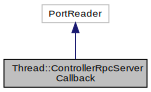
\includegraphics[width=224pt]{classThread_1_1ControllerRpcServerCallback__inherit__graph}
\end{center}
\end{figure}


Collaboration diagram for Thread\+:\+:Controller\+Rpc\+Server\+Callback\+:\nopagebreak
\begin{figure}[H]
\begin{center}
\leavevmode
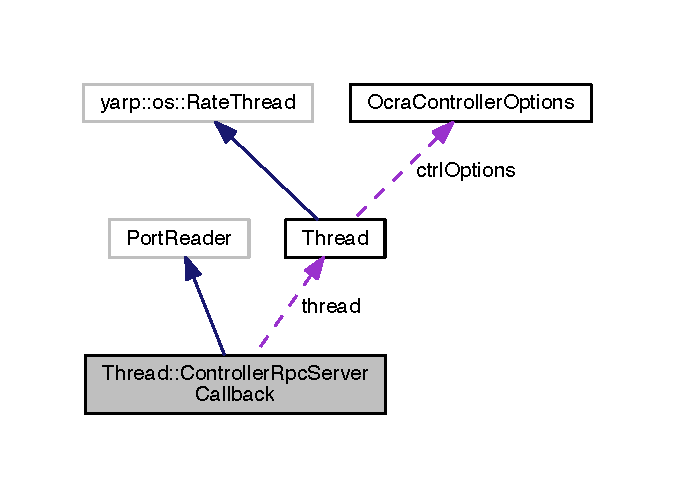
\includegraphics[width=324pt]{classThread_1_1ControllerRpcServerCallback__coll__graph}
\end{center}
\end{figure}
\subsection*{Public Member Functions}
\begin{DoxyCompactItemize}
\item 
\hyperlink{classThread_1_1ControllerRpcServerCallback_ad836e4cdaafc42ad309b5248ef38c280}{Controller\+Rpc\+Server\+Callback} (\hyperlink{classThread}{Thread} \&thread\+Ref)
\item 
virtual bool \hyperlink{classThread_1_1ControllerRpcServerCallback_a61f5510543f1bb96793dceca13eb6865}{read} (yarp\+::os\+::\+Connection\+Reader \&connection)
\end{DoxyCompactItemize}
\subsection*{Private Attributes}
\begin{DoxyCompactItemize}
\item 
\hyperlink{classThread}{Thread} \& \hyperlink{classThread_1_1ControllerRpcServerCallback_a466f100742fdac49e0016ec2f0c43536}{thread}
\end{DoxyCompactItemize}


\subsection{Detailed Description}
A callback function which binds the rpc server port opened in the contoller server module to the controller thread\textquotesingle{}s parsing function. 

\subsection{Constructor \& Destructor Documentation}
\hypertarget{classThread_1_1ControllerRpcServerCallback_ad836e4cdaafc42ad309b5248ef38c280}{}\label{classThread_1_1ControllerRpcServerCallback_ad836e4cdaafc42ad309b5248ef38c280} 
\index{Thread\+::\+Controller\+Rpc\+Server\+Callback@{Thread\+::\+Controller\+Rpc\+Server\+Callback}!Controller\+Rpc\+Server\+Callback@{Controller\+Rpc\+Server\+Callback}}
\index{Controller\+Rpc\+Server\+Callback@{Controller\+Rpc\+Server\+Callback}!Thread\+::\+Controller\+Rpc\+Server\+Callback@{Thread\+::\+Controller\+Rpc\+Server\+Callback}}
\subsubsection{\texorpdfstring{Controller\+Rpc\+Server\+Callback()}{ControllerRpcServerCallback()}}
{\footnotesize\ttfamily Thread\+::\+Controller\+Rpc\+Server\+Callback\+::\+Controller\+Rpc\+Server\+Callback (\begin{DoxyParamCaption}\item[{\hyperlink{classThread}{Thread} \&}]{thread\+Ref }\end{DoxyParamCaption})}

Constructor 
\begin{DoxyParams}{Parameters}
{\em ct\+Thread\+Ptr} & A shared pointer to the control thread. \\
\hline
\end{DoxyParams}


\subsection{Member Function Documentation}
\hypertarget{classThread_1_1ControllerRpcServerCallback_a61f5510543f1bb96793dceca13eb6865}{}\label{classThread_1_1ControllerRpcServerCallback_a61f5510543f1bb96793dceca13eb6865} 
\index{Thread\+::\+Controller\+Rpc\+Server\+Callback@{Thread\+::\+Controller\+Rpc\+Server\+Callback}!read@{read}}
\index{read@{read}!Thread\+::\+Controller\+Rpc\+Server\+Callback@{Thread\+::\+Controller\+Rpc\+Server\+Callback}}
\subsubsection{\texorpdfstring{read()}{read()}}
{\footnotesize\ttfamily bool Thread\+::\+Controller\+Rpc\+Server\+Callback\+::read (\begin{DoxyParamCaption}\item[{yarp\+::os\+::\+Connection\+Reader \&}]{connection }\end{DoxyParamCaption})\hspace{0.3cm}{\ttfamily [virtual]}}

read 
\begin{DoxyParams}{Parameters}
{\em connection} & Reads a port connection.\\
\hline
\end{DoxyParams}
\begin{DoxyReturn}{Returns}
A boolean which tells whether or not a message was read. 
\end{DoxyReturn}


\subsection{Member Data Documentation}
\hypertarget{classThread_1_1ControllerRpcServerCallback_a466f100742fdac49e0016ec2f0c43536}{}\label{classThread_1_1ControllerRpcServerCallback_a466f100742fdac49e0016ec2f0c43536} 
\index{Thread\+::\+Controller\+Rpc\+Server\+Callback@{Thread\+::\+Controller\+Rpc\+Server\+Callback}!thread@{thread}}
\index{thread@{thread}!Thread\+::\+Controller\+Rpc\+Server\+Callback@{Thread\+::\+Controller\+Rpc\+Server\+Callback}}
\subsubsection{\texorpdfstring{thread}{thread}}
{\footnotesize\ttfamily \hyperlink{classThread}{Thread}\& Thread\+::\+Controller\+Rpc\+Server\+Callback\+::thread\hspace{0.3cm}{\ttfamily [private]}}

A shared pointer to the control thread. 

The documentation for this class was generated from the following files\+:\begin{DoxyCompactItemize}
\item 
/\+Users/jorhabibeljaik/\+Code/codyco-\/superbuild/main/ocra-\/wbi-\/plugins/ocra-\/icub-\/server/include/ocra-\/icub-\/server/\hyperlink{Thread_8h}{Thread.\+h}\item 
/\+Users/jorhabibeljaik/\+Code/codyco-\/superbuild/main/ocra-\/wbi-\/plugins/ocra-\/icub-\/server/src/\hyperlink{Thread_8cpp}{Thread.\+cpp}\end{DoxyCompactItemize}

\hypertarget{classThread_1_1DebugRpcServerCallback}{}\section{Thread\+:\+:Debug\+Rpc\+Server\+Callback Class Reference}
\label{classThread_1_1DebugRpcServerCallback}\index{Thread\+::\+Debug\+Rpc\+Server\+Callback@{Thread\+::\+Debug\+Rpc\+Server\+Callback}}


A callback function which binds the rpc server port opened in the contoller server module to the controller thread\textquotesingle{}s parsing function.  




{\ttfamily \#include $<$Thread.\+h$>$}



Inheritance diagram for Thread\+:\+:Debug\+Rpc\+Server\+Callback\+:\nopagebreak
\begin{figure}[H]
\begin{center}
\leavevmode
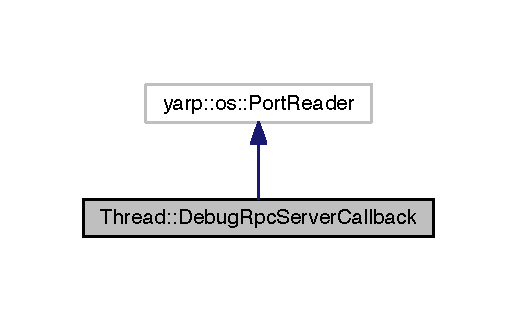
\includegraphics[width=248pt]{classThread_1_1DebugRpcServerCallback__inherit__graph}
\end{center}
\end{figure}


Collaboration diagram for Thread\+:\+:Debug\+Rpc\+Server\+Callback\+:\nopagebreak
\begin{figure}[H]
\begin{center}
\leavevmode
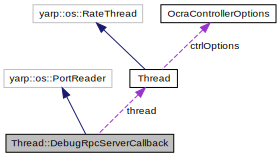
\includegraphics[width=350pt]{classThread_1_1DebugRpcServerCallback__coll__graph}
\end{center}
\end{figure}
\subsection*{Public Member Functions}
\begin{DoxyCompactItemize}
\item 
\hyperlink{classThread_1_1DebugRpcServerCallback_a479142cdf2f840df23b4605a532aaddf}{Debug\+Rpc\+Server\+Callback} (\hyperlink{classThread}{Thread} \&thread\+Ref)
\item 
virtual bool \hyperlink{classThread_1_1DebugRpcServerCallback_a3b39ac9b379ce3212bb2b05a89fa6024}{read} (yarp\+::os\+::\+Connection\+Reader \&connection)
\end{DoxyCompactItemize}
\subsection*{Private Attributes}
\begin{DoxyCompactItemize}
\item 
\hyperlink{classThread}{Thread} \& \hyperlink{classThread_1_1DebugRpcServerCallback_ad75683fc200019e8f681ad441b6ce84b}{thread}
\end{DoxyCompactItemize}


\subsection{Detailed Description}
A callback function which binds the rpc server port opened in the contoller server module to the controller thread\textquotesingle{}s parsing function. 

\subsection{Constructor \& Destructor Documentation}
\hypertarget{classThread_1_1DebugRpcServerCallback_a479142cdf2f840df23b4605a532aaddf}{}\label{classThread_1_1DebugRpcServerCallback_a479142cdf2f840df23b4605a532aaddf} 
\index{Thread\+::\+Debug\+Rpc\+Server\+Callback@{Thread\+::\+Debug\+Rpc\+Server\+Callback}!Debug\+Rpc\+Server\+Callback@{Debug\+Rpc\+Server\+Callback}}
\index{Debug\+Rpc\+Server\+Callback@{Debug\+Rpc\+Server\+Callback}!Thread\+::\+Debug\+Rpc\+Server\+Callback@{Thread\+::\+Debug\+Rpc\+Server\+Callback}}
\subsubsection{\texorpdfstring{Debug\+Rpc\+Server\+Callback()}{DebugRpcServerCallback()}}
{\footnotesize\ttfamily Thread\+::\+Debug\+Rpc\+Server\+Callback\+::\+Debug\+Rpc\+Server\+Callback (\begin{DoxyParamCaption}\item[{\hyperlink{classThread}{Thread} \&}]{thread\+Ref }\end{DoxyParamCaption})}

Constructor 
\begin{DoxyParams}{Parameters}
{\em ct\+Thread\+Ptr} & A shared pointer to the control thread. \\
\hline
\end{DoxyParams}


\subsection{Member Function Documentation}
\hypertarget{classThread_1_1DebugRpcServerCallback_a3b39ac9b379ce3212bb2b05a89fa6024}{}\label{classThread_1_1DebugRpcServerCallback_a3b39ac9b379ce3212bb2b05a89fa6024} 
\index{Thread\+::\+Debug\+Rpc\+Server\+Callback@{Thread\+::\+Debug\+Rpc\+Server\+Callback}!read@{read}}
\index{read@{read}!Thread\+::\+Debug\+Rpc\+Server\+Callback@{Thread\+::\+Debug\+Rpc\+Server\+Callback}}
\subsubsection{\texorpdfstring{read()}{read()}}
{\footnotesize\ttfamily bool Thread\+::\+Debug\+Rpc\+Server\+Callback\+::read (\begin{DoxyParamCaption}\item[{yarp\+::os\+::\+Connection\+Reader \&}]{connection }\end{DoxyParamCaption})\hspace{0.3cm}{\ttfamily [virtual]}}

read 
\begin{DoxyParams}{Parameters}
{\em connection} & Reads a port connection.\\
\hline
\end{DoxyParams}
\begin{DoxyReturn}{Returns}
A boolean which tells whether or not a message was read. 
\end{DoxyReturn}


\subsection{Member Data Documentation}
\hypertarget{classThread_1_1DebugRpcServerCallback_ad75683fc200019e8f681ad441b6ce84b}{}\label{classThread_1_1DebugRpcServerCallback_ad75683fc200019e8f681ad441b6ce84b} 
\index{Thread\+::\+Debug\+Rpc\+Server\+Callback@{Thread\+::\+Debug\+Rpc\+Server\+Callback}!thread@{thread}}
\index{thread@{thread}!Thread\+::\+Debug\+Rpc\+Server\+Callback@{Thread\+::\+Debug\+Rpc\+Server\+Callback}}
\subsubsection{\texorpdfstring{thread}{thread}}
{\footnotesize\ttfamily \hyperlink{classThread}{Thread}\& Thread\+::\+Debug\+Rpc\+Server\+Callback\+::thread\hspace{0.3cm}{\ttfamily [private]}}

A shared pointer to the control thread. 

The documentation for this class was generated from the following files\+:\begin{DoxyCompactItemize}
\item 
/\+Users/jorhabibeljaik/\+Code/codyco-\/superbuild/main/ocra-\/wbi-\/plugins/ocra-\/icub-\/server/include/ocra-\/icub-\/server/\hyperlink{Thread_8h}{Thread.\+h}\item 
/\+Users/jorhabibeljaik/\+Code/codyco-\/superbuild/main/ocra-\/wbi-\/plugins/ocra-\/icub-\/server/src/\hyperlink{Thread_8cpp}{Thread.\+cpp}\end{DoxyCompactItemize}

\hypertarget{classExampleClient}{}\section{Example\+Client Class Reference}
\label{classExampleClient}\index{Example\+Client@{Example\+Client}}


{\ttfamily \#include $<$Example\+Client.\+h$>$}



Inheritance diagram for Example\+Client\+:\nopagebreak
\begin{figure}[H]
\begin{center}
\leavevmode
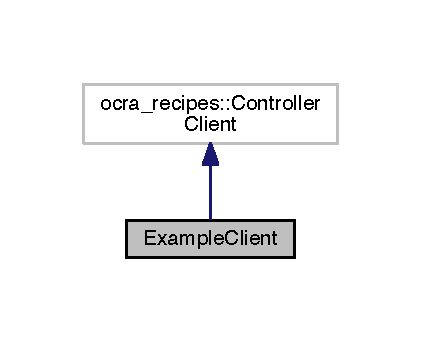
\includegraphics[width=202pt]{classExampleClient__inherit__graph}
\end{center}
\end{figure}


Collaboration diagram for Example\+Client\+:\nopagebreak
\begin{figure}[H]
\begin{center}
\leavevmode
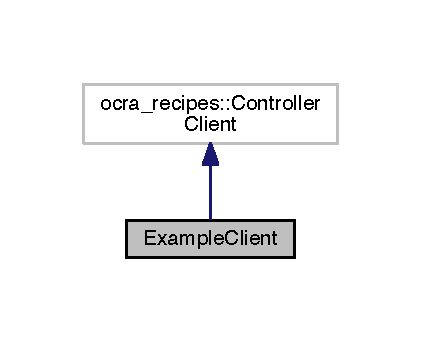
\includegraphics[width=202pt]{classExampleClient__coll__graph}
\end{center}
\end{figure}
\subsection*{Public Member Functions}
\begin{DoxyCompactItemize}
\item 
\hyperlink{classExampleClient_aed7d851662cba1484ecf1db8161d6e62}{Example\+Client} (std\+::shared\+\_\+ptr$<$ ocra\+::\+Model $>$ model\+Ptr, const int loop\+Period)
\item 
virtual \hyperlink{classExampleClient_abdca7dbe5fdab81d7d661a677e5ccd14}{$\sim$\+Example\+Client} ()
\end{DoxyCompactItemize}
\subsection*{Protected Member Functions}
\begin{DoxyCompactItemize}
\item 
virtual bool \hyperlink{classExampleClient_ad504d1d87997fc95bfeca6aa925a4fa6}{initialize} ()
\item 
virtual void \hyperlink{classExampleClient_a5acf25784c1c5b51c2c085327f195002}{release} ()
\item 
virtual void \hyperlink{classExampleClient_afb58f3425aafe2d4c38195cb3c667dbc}{loop} ()
\end{DoxyCompactItemize}
\subsection*{Private Attributes}
\begin{DoxyCompactItemize}
\item 
double \hyperlink{classExampleClient_aaa5ec782e9aaa1e94d7182872f743c02}{start\+Time}
\item 
double \hyperlink{classExampleClient_acade7035d4e39290cbda08b98249a629}{wait\+Time}
\item 
bool \hyperlink{classExampleClient_a90ce0c4d970c903b3e6afb6f5ca2a228}{trigger}
\item 
bool \hyperlink{classExampleClient_acd2cf0f0479ff8bbf5b64924d83beb60}{done}
\item 
Eigen\+::\+Matrix\+Xd \hyperlink{classExampleClient_acf4657277ecb08168d9a17c208814823}{waypoints}
\item 
std\+::shared\+\_\+ptr$<$ ocra\+\_\+recipes\+::\+Trajectory\+Thread $>$ \hyperlink{classExampleClient_a4311b0e8c4878c23df2b5ba048d8bc05}{left\+Hand\+Traj\+Thread}
\item 
bool \hyperlink{classExampleClient_a7fb2b50cbdac0ec3a32e44b5bbc3b11f}{p1}
\item 
bool \hyperlink{classExampleClient_a07c2bc5c5c522e77a726017c28db2ec9}{p2}
\item 
bool \hyperlink{classExampleClient_ab41df6f34a51e649051adbac6d3077f9}{p3}
\end{DoxyCompactItemize}


\subsection{Constructor \& Destructor Documentation}
\hypertarget{classExampleClient_aed7d851662cba1484ecf1db8161d6e62}{}\label{classExampleClient_aed7d851662cba1484ecf1db8161d6e62} 
\index{Example\+Client@{Example\+Client}!Example\+Client@{Example\+Client}}
\index{Example\+Client@{Example\+Client}!Example\+Client@{Example\+Client}}
\subsubsection{\texorpdfstring{Example\+Client()}{ExampleClient()}}
{\footnotesize\ttfamily Example\+Client\+::\+Example\+Client (\begin{DoxyParamCaption}\item[{std\+::shared\+\_\+ptr$<$ ocra\+::\+Model $>$}]{model\+Ptr,  }\item[{const int}]{loop\+Period }\end{DoxyParamCaption})}

\hypertarget{classExampleClient_abdca7dbe5fdab81d7d661a677e5ccd14}{}\label{classExampleClient_abdca7dbe5fdab81d7d661a677e5ccd14} 
\index{Example\+Client@{Example\+Client}!````~Example\+Client@{$\sim$\+Example\+Client}}
\index{````~Example\+Client@{$\sim$\+Example\+Client}!Example\+Client@{Example\+Client}}
\subsubsection{\texorpdfstring{$\sim$\+Example\+Client()}{~ExampleClient()}}
{\footnotesize\ttfamily Example\+Client\+::$\sim$\+Example\+Client (\begin{DoxyParamCaption}{ }\end{DoxyParamCaption})\hspace{0.3cm}{\ttfamily [virtual]}}



\subsection{Member Function Documentation}
\hypertarget{classExampleClient_ad504d1d87997fc95bfeca6aa925a4fa6}{}\label{classExampleClient_ad504d1d87997fc95bfeca6aa925a4fa6} 
\index{Example\+Client@{Example\+Client}!initialize@{initialize}}
\index{initialize@{initialize}!Example\+Client@{Example\+Client}}
\subsubsection{\texorpdfstring{initialize()}{initialize()}}
{\footnotesize\ttfamily bool Example\+Client\+::initialize (\begin{DoxyParamCaption}{ }\end{DoxyParamCaption})\hspace{0.3cm}{\ttfamily [protected]}, {\ttfamily [virtual]}}

\hypertarget{classExampleClient_afb58f3425aafe2d4c38195cb3c667dbc}{}\label{classExampleClient_afb58f3425aafe2d4c38195cb3c667dbc} 
\index{Example\+Client@{Example\+Client}!loop@{loop}}
\index{loop@{loop}!Example\+Client@{Example\+Client}}
\subsubsection{\texorpdfstring{loop()}{loop()}}
{\footnotesize\ttfamily void Example\+Client\+::loop (\begin{DoxyParamCaption}{ }\end{DoxyParamCaption})\hspace{0.3cm}{\ttfamily [protected]}, {\ttfamily [virtual]}}

\hypertarget{classExampleClient_a5acf25784c1c5b51c2c085327f195002}{}\label{classExampleClient_a5acf25784c1c5b51c2c085327f195002} 
\index{Example\+Client@{Example\+Client}!release@{release}}
\index{release@{release}!Example\+Client@{Example\+Client}}
\subsubsection{\texorpdfstring{release()}{release()}}
{\footnotesize\ttfamily void Example\+Client\+::release (\begin{DoxyParamCaption}{ }\end{DoxyParamCaption})\hspace{0.3cm}{\ttfamily [protected]}, {\ttfamily [virtual]}}



\subsection{Member Data Documentation}
\hypertarget{classExampleClient_acd2cf0f0479ff8bbf5b64924d83beb60}{}\label{classExampleClient_acd2cf0f0479ff8bbf5b64924d83beb60} 
\index{Example\+Client@{Example\+Client}!done@{done}}
\index{done@{done}!Example\+Client@{Example\+Client}}
\subsubsection{\texorpdfstring{done}{done}}
{\footnotesize\ttfamily bool Example\+Client\+::done\hspace{0.3cm}{\ttfamily [private]}}

\hypertarget{classExampleClient_a4311b0e8c4878c23df2b5ba048d8bc05}{}\label{classExampleClient_a4311b0e8c4878c23df2b5ba048d8bc05} 
\index{Example\+Client@{Example\+Client}!left\+Hand\+Traj\+Thread@{left\+Hand\+Traj\+Thread}}
\index{left\+Hand\+Traj\+Thread@{left\+Hand\+Traj\+Thread}!Example\+Client@{Example\+Client}}
\subsubsection{\texorpdfstring{left\+Hand\+Traj\+Thread}{leftHandTrajThread}}
{\footnotesize\ttfamily std\+::shared\+\_\+ptr$<$ocra\+\_\+recipes\+::\+Trajectory\+Thread$>$ Example\+Client\+::left\+Hand\+Traj\+Thread\hspace{0.3cm}{\ttfamily [private]}}

\hypertarget{classExampleClient_a7fb2b50cbdac0ec3a32e44b5bbc3b11f}{}\label{classExampleClient_a7fb2b50cbdac0ec3a32e44b5bbc3b11f} 
\index{Example\+Client@{Example\+Client}!p1@{p1}}
\index{p1@{p1}!Example\+Client@{Example\+Client}}
\subsubsection{\texorpdfstring{p1}{p1}}
{\footnotesize\ttfamily bool Example\+Client\+::p1\hspace{0.3cm}{\ttfamily [private]}}

\hypertarget{classExampleClient_a07c2bc5c5c522e77a726017c28db2ec9}{}\label{classExampleClient_a07c2bc5c5c522e77a726017c28db2ec9} 
\index{Example\+Client@{Example\+Client}!p2@{p2}}
\index{p2@{p2}!Example\+Client@{Example\+Client}}
\subsubsection{\texorpdfstring{p2}{p2}}
{\footnotesize\ttfamily bool Example\+Client\+::p2\hspace{0.3cm}{\ttfamily [private]}}

\hypertarget{classExampleClient_ab41df6f34a51e649051adbac6d3077f9}{}\label{classExampleClient_ab41df6f34a51e649051adbac6d3077f9} 
\index{Example\+Client@{Example\+Client}!p3@{p3}}
\index{p3@{p3}!Example\+Client@{Example\+Client}}
\subsubsection{\texorpdfstring{p3}{p3}}
{\footnotesize\ttfamily bool Example\+Client\+::p3\hspace{0.3cm}{\ttfamily [private]}}

\hypertarget{classExampleClient_aaa5ec782e9aaa1e94d7182872f743c02}{}\label{classExampleClient_aaa5ec782e9aaa1e94d7182872f743c02} 
\index{Example\+Client@{Example\+Client}!start\+Time@{start\+Time}}
\index{start\+Time@{start\+Time}!Example\+Client@{Example\+Client}}
\subsubsection{\texorpdfstring{start\+Time}{startTime}}
{\footnotesize\ttfamily double Example\+Client\+::start\+Time\hspace{0.3cm}{\ttfamily [private]}}

\hypertarget{classExampleClient_a90ce0c4d970c903b3e6afb6f5ca2a228}{}\label{classExampleClient_a90ce0c4d970c903b3e6afb6f5ca2a228} 
\index{Example\+Client@{Example\+Client}!trigger@{trigger}}
\index{trigger@{trigger}!Example\+Client@{Example\+Client}}
\subsubsection{\texorpdfstring{trigger}{trigger}}
{\footnotesize\ttfamily bool Example\+Client\+::trigger\hspace{0.3cm}{\ttfamily [private]}}

\hypertarget{classExampleClient_acade7035d4e39290cbda08b98249a629}{}\label{classExampleClient_acade7035d4e39290cbda08b98249a629} 
\index{Example\+Client@{Example\+Client}!wait\+Time@{wait\+Time}}
\index{wait\+Time@{wait\+Time}!Example\+Client@{Example\+Client}}
\subsubsection{\texorpdfstring{wait\+Time}{waitTime}}
{\footnotesize\ttfamily double Example\+Client\+::wait\+Time\hspace{0.3cm}{\ttfamily [private]}}

\hypertarget{classExampleClient_acf4657277ecb08168d9a17c208814823}{}\label{classExampleClient_acf4657277ecb08168d9a17c208814823} 
\index{Example\+Client@{Example\+Client}!waypoints@{waypoints}}
\index{waypoints@{waypoints}!Example\+Client@{Example\+Client}}
\subsubsection{\texorpdfstring{waypoints}{waypoints}}
{\footnotesize\ttfamily Eigen\+::\+Matrix\+Xd Example\+Client\+::waypoints\hspace{0.3cm}{\ttfamily [private]}}



The documentation for this class was generated from the following files\+:\begin{DoxyCompactItemize}
\item 
/\+Users/jorhabibeljaik/\+Code/codyco-\/superbuild/main/ocra-\/wbi-\/plugins/ocra-\/icub-\/clients/example-\/client/include/example-\/client/\hyperlink{ExampleClient_8h}{Example\+Client.\+h}\item 
/\+Users/jorhabibeljaik/\+Code/codyco-\/superbuild/main/ocra-\/wbi-\/plugins/ocra-\/icub-\/clients/example-\/client/src/\hyperlink{ExampleClient_8cpp}{Example\+Client.\+cpp}\end{DoxyCompactItemize}

\hypertarget{classIcubControllerServer}{}\section{Icub\+Controller\+Server Class Reference}
\label{classIcubControllerServer}\index{Icub\+Controller\+Server@{Icub\+Controller\+Server}}


{\ttfamily \#include $<$Icub\+Controller\+Server.\+h$>$}



Inheritance diagram for Icub\+Controller\+Server\+:\nopagebreak
\begin{figure}[H]
\begin{center}
\leavevmode
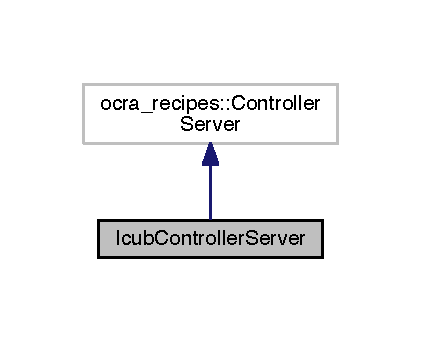
\includegraphics[width=202pt]{classIcubControllerServer__inherit__graph}
\end{center}
\end{figure}


Collaboration diagram for Icub\+Controller\+Server\+:\nopagebreak
\begin{figure}[H]
\begin{center}
\leavevmode
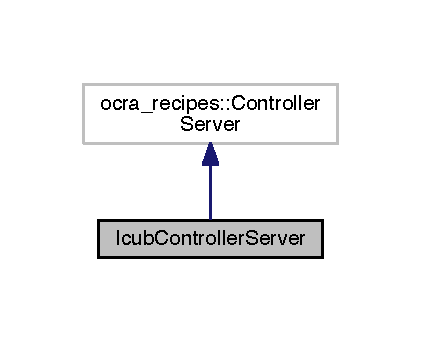
\includegraphics[width=202pt]{classIcubControllerServer__coll__graph}
\end{center}
\end{figure}
\subsection*{Public Member Functions}
\begin{DoxyCompactItemize}
\item 
\hyperlink{classIcubControllerServer_a6b0a6021e3c82e72ac97ad30d3f0c082}{Icub\+Controller\+Server} (std\+::shared\+\_\+ptr$<$ wbi\+::whole\+Body\+Interface $>$ robot, std\+::string icub\+Name, const bool using\+Floating\+Base, const ocra\+\_\+recipes\+::\+C\+O\+N\+T\+R\+O\+L\+L\+E\+R\+\_\+\+T\+Y\+PE ctrl\+Type=ocra\+\_\+recipes\+::\+W\+O\+C\+R\+A\+\_\+\+C\+O\+N\+T\+R\+O\+L\+L\+ER, const ocra\+\_\+recipes\+::\+S\+O\+L\+V\+E\+R\+\_\+\+T\+Y\+PE solver=ocra\+\_\+recipes\+::\+Q\+U\+A\+D\+P\+R\+OG, const bool using\+Interprocess\+Communication=true, const bool \hyperlink{classIcubControllerServer_adc410f503b14ed288c01e877ac405114}{use\+Odometry}=false)
\item 
virtual \hyperlink{classIcubControllerServer_a7582d4bbf9851ee9b58913ea2a89e5fd}{$\sim$\+Icub\+Controller\+Server} ()
\item 
virtual ocra\+::\+Model\+::\+Ptr \hyperlink{classIcubControllerServer_a025d8e257a69ef3d2c5a10b3cbfe2350}{load\+Robot\+Model} ()
\item 
virtual void \hyperlink{classIcubControllerServer_ac068c7930f342bb0cb0969d0d04267cf}{get\+Robot\+State} (Eigen\+::\+Vector\+Xd \&q, Eigen\+::\+Vector\+Xd \&qd, Eigen\+::\+Displacementd \&H\+\_\+root, Eigen\+::\+Twistd \&T\+\_\+root)
\item 
bool \hyperlink{classIcubControllerServer_a810f139a27e06458549ccbb3fde12359}{initialize\+Odometry} (std\+::string model\+\_\+file, std\+::string initial\+Fixed\+Frame)
\item 
std\+::vector$<$ std\+::string $>$ \hyperlink{classIcubControllerServer_a892bb43e568d3f112465dff1e0c6b348}{get\+Canonical\+\_\+i\+Cub\+Joints} ()
\item 
void \hyperlink{classIcubControllerServer_a032c035880f8ec2b77ef14521be6e75a}{root\+Frame\+Velocity} (Eigen\+::\+Vector\+Xd \&q, Eigen\+::\+Vector\+Xd \&qd, i\+Dyn\+Tree\+::\+Transform \&wbi\+\_\+\+H\+\_\+root\+\_\+\+Transform, double regularization, int L\+E\+F\+T\+\_\+\+F\+O\+O\+T\+\_\+\+C\+O\+N\+T\+A\+CT, int R\+I\+G\+H\+T\+\_\+\+F\+O\+O\+T\+\_\+\+C\+O\+N\+T\+A\+CT, Eigen\+::\+Vector\+Xd \&twist)
\item 
void \hyperlink{classIcubControllerServer_a27211ecba9fc8618733bcaea9ff7d140}{root\+Frame\+Velocity\+Piv\+LU} (Eigen\+::\+Vector\+Xd \&q, Eigen\+::\+Vector\+Xd \&qd, i\+Dyn\+Tree\+::\+Transform \&wbi\+\_\+\+H\+\_\+root\+\_\+\+Transform, Eigen\+::\+Vector\+Xd \&twist)
\item 
void \hyperlink{classIcubControllerServer_a82650f373c3c2c52a91cc744c67b0dcf}{root\+Frame\+Velocity\+Piv\+LU} (Eigen\+::\+Vector\+Xd \&q, Eigen\+::\+Vector\+Xd \&qd, i\+Dyn\+Tree\+::\+Transform \&wbi\+\_\+\+H\+\_\+root\+\_\+\+Transform, int L\+E\+F\+T\+\_\+\+F\+O\+O\+T\+\_\+\+C\+O\+N\+T\+A\+CT, int R\+I\+G\+H\+T\+\_\+\+F\+O\+O\+T\+\_\+\+C\+O\+N\+T\+A\+CT, Eigen\+::\+Vector\+Xd \&twist)
\item 
void \hyperlink{classIcubControllerServer_af43586b816992e5e7fceac5a7245f673}{pinv} (Eigen\+::\+Matrix\+Xd mat, Eigen\+::\+Matrix\+Xd \&pinvmat, double pinvtoler=1.\+0e-\/6) const
\item 
void \hyperlink{classIcubControllerServer_aaedff28c5d9ac9a7cdbc24c9e0cbc5b3}{velocity\+Error} (Eigen\+::\+Matrix\+Xd A, Eigen\+::\+Matrix\+Xd B, Eigen\+::\+Matrix\+Xd X)
\end{DoxyCompactItemize}
\subsection*{Private Attributes}
\begin{DoxyCompactItemize}
\item 
std\+::shared\+\_\+ptr$<$ wbi\+::whole\+Body\+Interface $>$ \hyperlink{classIcubControllerServer_ae8a89707675adb58bb3006bc085828b7}{wbi}
\item 
std\+::string \hyperlink{classIcubControllerServer_a041d6687258c36677914b1d15f18e153}{robot\+Name}
\item 
bool \hyperlink{classIcubControllerServer_aebc2019921c3eabb53c01012fbd2355a}{is\+Floating\+Base}
\item 
bool \hyperlink{classIcubControllerServer_adc410f503b14ed288c01e877ac405114}{use\+Odometry}
\item 
int \hyperlink{classIcubControllerServer_ab5fb1f18775cfe3036894c73dc21ebcf}{n\+DoF}
\item 
Eigen\+::\+Vector\+Xd \hyperlink{classIcubControllerServer_a42f6a8db660da9dbafbc57941b1ee12f}{wbi\+\_\+\+H\+\_\+root\+\_\+\+Vector}
\item 
Eigen\+::\+Vector\+Xd \hyperlink{classIcubControllerServer_a818b66e75b7f9457a6a5bcbb3c1306a7}{wbi\+\_\+\+T\+\_\+root\+\_\+\+Vector}
\item 
wbi\+::\+Frame \hyperlink{classIcubControllerServer_afd983b69c043eedf958e53582b22195a}{wbi\+\_\+\+H\+\_\+root}
\item 
i\+Dyn\+Tree\+::\+Simple\+Legged\+Odometry \hyperlink{classIcubControllerServer_ad0484106ab9d7fd42e2bd682338871c7}{odometry}
\end{DoxyCompactItemize}
\subsection*{Static Private Attributes}
\begin{DoxyCompactItemize}
\item 
static const int \hyperlink{classIcubControllerServer_aa977ca558c184e4331121522cc58d2e7}{A\+L\+L\+\_\+\+J\+O\+I\+N\+TS} = -\/1
\end{DoxyCompactItemize}


\subsection{Constructor \& Destructor Documentation}
\hypertarget{classIcubControllerServer_a6b0a6021e3c82e72ac97ad30d3f0c082}{}\label{classIcubControllerServer_a6b0a6021e3c82e72ac97ad30d3f0c082} 
\index{Icub\+Controller\+Server@{Icub\+Controller\+Server}!Icub\+Controller\+Server@{Icub\+Controller\+Server}}
\index{Icub\+Controller\+Server@{Icub\+Controller\+Server}!Icub\+Controller\+Server@{Icub\+Controller\+Server}}
\subsubsection{\texorpdfstring{Icub\+Controller\+Server()}{IcubControllerServer()}}
{\footnotesize\ttfamily Icub\+Controller\+Server\+::\+Icub\+Controller\+Server (\begin{DoxyParamCaption}\item[{std\+::shared\+\_\+ptr$<$ wbi\+::whole\+Body\+Interface $>$}]{robot,  }\item[{std\+::string}]{icub\+Name,  }\item[{const bool}]{using\+Floating\+Base,  }\item[{const ocra\+\_\+recipes\+::\+C\+O\+N\+T\+R\+O\+L\+L\+E\+R\+\_\+\+T\+Y\+PE}]{ctrl\+Type = {\ttfamily ocra\+\_\+recipes\+:\+:WOCRA\+\_\+CONTROLLER},  }\item[{const ocra\+\_\+recipes\+::\+S\+O\+L\+V\+E\+R\+\_\+\+T\+Y\+PE}]{solver = {\ttfamily ocra\+\_\+recipes\+:\+:QUADPROG},  }\item[{const bool}]{using\+Interprocess\+Communication = {\ttfamily true},  }\item[{const bool}]{use\+Odometry = {\ttfamily false} }\end{DoxyParamCaption})}

\hypertarget{classIcubControllerServer_a7582d4bbf9851ee9b58913ea2a89e5fd}{}\label{classIcubControllerServer_a7582d4bbf9851ee9b58913ea2a89e5fd} 
\index{Icub\+Controller\+Server@{Icub\+Controller\+Server}!````~Icub\+Controller\+Server@{$\sim$\+Icub\+Controller\+Server}}
\index{````~Icub\+Controller\+Server@{$\sim$\+Icub\+Controller\+Server}!Icub\+Controller\+Server@{Icub\+Controller\+Server}}
\subsubsection{\texorpdfstring{$\sim$\+Icub\+Controller\+Server()}{~IcubControllerServer()}}
{\footnotesize\ttfamily Icub\+Controller\+Server\+::$\sim$\+Icub\+Controller\+Server (\begin{DoxyParamCaption}{ }\end{DoxyParamCaption})\hspace{0.3cm}{\ttfamily [virtual]}}



\subsection{Member Function Documentation}
\hypertarget{classIcubControllerServer_a892bb43e568d3f112465dff1e0c6b348}{}\label{classIcubControllerServer_a892bb43e568d3f112465dff1e0c6b348} 
\index{Icub\+Controller\+Server@{Icub\+Controller\+Server}!get\+Canonical\+\_\+i\+Cub\+Joints@{get\+Canonical\+\_\+i\+Cub\+Joints}}
\index{get\+Canonical\+\_\+i\+Cub\+Joints@{get\+Canonical\+\_\+i\+Cub\+Joints}!Icub\+Controller\+Server@{Icub\+Controller\+Server}}
\subsubsection{\texorpdfstring{get\+Canonical\+\_\+i\+Cub\+Joints()}{getCanonical\_iCubJoints()}}
{\footnotesize\ttfamily std\+::vector$<$ std\+::string $>$ Icub\+Controller\+Server\+::get\+Canonical\+\_\+i\+Cub\+Joints (\begin{DoxyParamCaption}{ }\end{DoxyParamCaption})}

\hypertarget{classIcubControllerServer_ac068c7930f342bb0cb0969d0d04267cf}{}\label{classIcubControllerServer_ac068c7930f342bb0cb0969d0d04267cf} 
\index{Icub\+Controller\+Server@{Icub\+Controller\+Server}!get\+Robot\+State@{get\+Robot\+State}}
\index{get\+Robot\+State@{get\+Robot\+State}!Icub\+Controller\+Server@{Icub\+Controller\+Server}}
\subsubsection{\texorpdfstring{get\+Robot\+State()}{getRobotState()}}
{\footnotesize\ttfamily void Icub\+Controller\+Server\+::get\+Robot\+State (\begin{DoxyParamCaption}\item[{Eigen\+::\+Vector\+Xd \&}]{q,  }\item[{Eigen\+::\+Vector\+Xd \&}]{qd,  }\item[{Eigen\+::\+Displacementd \&}]{H\+\_\+root,  }\item[{Eigen\+::\+Twistd \&}]{T\+\_\+root }\end{DoxyParamCaption})\hspace{0.3cm}{\ttfamily [virtual]}}

\hypertarget{classIcubControllerServer_a810f139a27e06458549ccbb3fde12359}{}\label{classIcubControllerServer_a810f139a27e06458549ccbb3fde12359} 
\index{Icub\+Controller\+Server@{Icub\+Controller\+Server}!initialize\+Odometry@{initialize\+Odometry}}
\index{initialize\+Odometry@{initialize\+Odometry}!Icub\+Controller\+Server@{Icub\+Controller\+Server}}
\subsubsection{\texorpdfstring{initialize\+Odometry()}{initializeOdometry()}}
{\footnotesize\ttfamily bool Icub\+Controller\+Server\+::initialize\+Odometry (\begin{DoxyParamCaption}\item[{std\+::string}]{model\+\_\+file,  }\item[{std\+::string}]{initial\+Fixed\+Frame }\end{DoxyParamCaption})}

\hypertarget{classIcubControllerServer_a025d8e257a69ef3d2c5a10b3cbfe2350}{}\label{classIcubControllerServer_a025d8e257a69ef3d2c5a10b3cbfe2350} 
\index{Icub\+Controller\+Server@{Icub\+Controller\+Server}!load\+Robot\+Model@{load\+Robot\+Model}}
\index{load\+Robot\+Model@{load\+Robot\+Model}!Icub\+Controller\+Server@{Icub\+Controller\+Server}}
\subsubsection{\texorpdfstring{load\+Robot\+Model()}{loadRobotModel()}}
{\footnotesize\ttfamily ocra\+::\+Model\+::\+Ptr Icub\+Controller\+Server\+::load\+Robot\+Model (\begin{DoxyParamCaption}{ }\end{DoxyParamCaption})\hspace{0.3cm}{\ttfamily [virtual]}}

\hypertarget{classIcubControllerServer_af43586b816992e5e7fceac5a7245f673}{}\label{classIcubControllerServer_af43586b816992e5e7fceac5a7245f673} 
\index{Icub\+Controller\+Server@{Icub\+Controller\+Server}!pinv@{pinv}}
\index{pinv@{pinv}!Icub\+Controller\+Server@{Icub\+Controller\+Server}}
\subsubsection{\texorpdfstring{pinv()}{pinv()}}
{\footnotesize\ttfamily void Icub\+Controller\+Server\+::pinv (\begin{DoxyParamCaption}\item[{Eigen\+::\+Matrix\+Xd}]{mat,  }\item[{Eigen\+::\+Matrix\+Xd \&}]{pinvmat,  }\item[{double}]{pinvtoler = {\ttfamily 1.0e-\/6} }\end{DoxyParamCaption}) const}

\hypertarget{classIcubControllerServer_a032c035880f8ec2b77ef14521be6e75a}{}\label{classIcubControllerServer_a032c035880f8ec2b77ef14521be6e75a} 
\index{Icub\+Controller\+Server@{Icub\+Controller\+Server}!root\+Frame\+Velocity@{root\+Frame\+Velocity}}
\index{root\+Frame\+Velocity@{root\+Frame\+Velocity}!Icub\+Controller\+Server@{Icub\+Controller\+Server}}
\subsubsection{\texorpdfstring{root\+Frame\+Velocity()}{rootFrameVelocity()}}
{\footnotesize\ttfamily void Icub\+Controller\+Server\+::root\+Frame\+Velocity (\begin{DoxyParamCaption}\item[{Eigen\+::\+Vector\+Xd \&}]{q,  }\item[{Eigen\+::\+Vector\+Xd \&}]{qd,  }\item[{i\+Dyn\+Tree\+::\+Transform \&}]{wbi\+\_\+\+H\+\_\+root\+\_\+\+Transform,  }\item[{double}]{regularization,  }\item[{int}]{L\+E\+F\+T\+\_\+\+F\+O\+O\+T\+\_\+\+C\+O\+N\+T\+A\+CT,  }\item[{int}]{R\+I\+G\+H\+T\+\_\+\+F\+O\+O\+T\+\_\+\+C\+O\+N\+T\+A\+CT,  }\item[{Eigen\+::\+Vector\+Xd \&}]{twist }\end{DoxyParamCaption})}

\hypertarget{classIcubControllerServer_a27211ecba9fc8618733bcaea9ff7d140}{}\label{classIcubControllerServer_a27211ecba9fc8618733bcaea9ff7d140} 
\index{Icub\+Controller\+Server@{Icub\+Controller\+Server}!root\+Frame\+Velocity\+Piv\+LU@{root\+Frame\+Velocity\+Piv\+LU}}
\index{root\+Frame\+Velocity\+Piv\+LU@{root\+Frame\+Velocity\+Piv\+LU}!Icub\+Controller\+Server@{Icub\+Controller\+Server}}
\subsubsection{\texorpdfstring{root\+Frame\+Velocity\+Piv\+L\+U()}{rootFrameVelocityPivLU()}\hspace{0.1cm}{\footnotesize\ttfamily [1/2]}}
{\footnotesize\ttfamily void Icub\+Controller\+Server\+::root\+Frame\+Velocity\+Piv\+LU (\begin{DoxyParamCaption}\item[{Eigen\+::\+Vector\+Xd \&}]{q,  }\item[{Eigen\+::\+Vector\+Xd \&}]{qd,  }\item[{i\+Dyn\+Tree\+::\+Transform \&}]{wbi\+\_\+\+H\+\_\+root\+\_\+\+Transform,  }\item[{Eigen\+::\+Vector\+Xd \&}]{twist }\end{DoxyParamCaption})}

\hypertarget{classIcubControllerServer_a82650f373c3c2c52a91cc744c67b0dcf}{}\label{classIcubControllerServer_a82650f373c3c2c52a91cc744c67b0dcf} 
\index{Icub\+Controller\+Server@{Icub\+Controller\+Server}!root\+Frame\+Velocity\+Piv\+LU@{root\+Frame\+Velocity\+Piv\+LU}}
\index{root\+Frame\+Velocity\+Piv\+LU@{root\+Frame\+Velocity\+Piv\+LU}!Icub\+Controller\+Server@{Icub\+Controller\+Server}}
\subsubsection{\texorpdfstring{root\+Frame\+Velocity\+Piv\+L\+U()}{rootFrameVelocityPivLU()}\hspace{0.1cm}{\footnotesize\ttfamily [2/2]}}
{\footnotesize\ttfamily void Icub\+Controller\+Server\+::root\+Frame\+Velocity\+Piv\+LU (\begin{DoxyParamCaption}\item[{Eigen\+::\+Vector\+Xd \&}]{q,  }\item[{Eigen\+::\+Vector\+Xd \&}]{qd,  }\item[{i\+Dyn\+Tree\+::\+Transform \&}]{wbi\+\_\+\+H\+\_\+root\+\_\+\+Transform,  }\item[{int}]{L\+E\+F\+T\+\_\+\+F\+O\+O\+T\+\_\+\+C\+O\+N\+T\+A\+CT,  }\item[{int}]{R\+I\+G\+H\+T\+\_\+\+F\+O\+O\+T\+\_\+\+C\+O\+N\+T\+A\+CT,  }\item[{Eigen\+::\+Vector\+Xd \&}]{twist }\end{DoxyParamCaption})}

\hypertarget{classIcubControllerServer_aaedff28c5d9ac9a7cdbc24c9e0cbc5b3}{}\label{classIcubControllerServer_aaedff28c5d9ac9a7cdbc24c9e0cbc5b3} 
\index{Icub\+Controller\+Server@{Icub\+Controller\+Server}!velocity\+Error@{velocity\+Error}}
\index{velocity\+Error@{velocity\+Error}!Icub\+Controller\+Server@{Icub\+Controller\+Server}}
\subsubsection{\texorpdfstring{velocity\+Error()}{velocityError()}}
{\footnotesize\ttfamily void Icub\+Controller\+Server\+::velocity\+Error (\begin{DoxyParamCaption}\item[{Eigen\+::\+Matrix\+Xd}]{A,  }\item[{Eigen\+::\+Matrix\+Xd}]{B,  }\item[{Eigen\+::\+Matrix\+Xd}]{X }\end{DoxyParamCaption})}



\subsection{Member Data Documentation}
\hypertarget{classIcubControllerServer_aa977ca558c184e4331121522cc58d2e7}{}\label{classIcubControllerServer_aa977ca558c184e4331121522cc58d2e7} 
\index{Icub\+Controller\+Server@{Icub\+Controller\+Server}!A\+L\+L\+\_\+\+J\+O\+I\+N\+TS@{A\+L\+L\+\_\+\+J\+O\+I\+N\+TS}}
\index{A\+L\+L\+\_\+\+J\+O\+I\+N\+TS@{A\+L\+L\+\_\+\+J\+O\+I\+N\+TS}!Icub\+Controller\+Server@{Icub\+Controller\+Server}}
\subsubsection{\texorpdfstring{A\+L\+L\+\_\+\+J\+O\+I\+N\+TS}{ALL\_JOINTS}}
{\footnotesize\ttfamily const int Icub\+Controller\+Server\+::\+A\+L\+L\+\_\+\+J\+O\+I\+N\+TS = -\/1\hspace{0.3cm}{\ttfamily [static]}, {\ttfamily [private]}}

\hypertarget{classIcubControllerServer_aebc2019921c3eabb53c01012fbd2355a}{}\label{classIcubControllerServer_aebc2019921c3eabb53c01012fbd2355a} 
\index{Icub\+Controller\+Server@{Icub\+Controller\+Server}!is\+Floating\+Base@{is\+Floating\+Base}}
\index{is\+Floating\+Base@{is\+Floating\+Base}!Icub\+Controller\+Server@{Icub\+Controller\+Server}}
\subsubsection{\texorpdfstring{is\+Floating\+Base}{isFloatingBase}}
{\footnotesize\ttfamily bool Icub\+Controller\+Server\+::is\+Floating\+Base\hspace{0.3cm}{\ttfamily [private]}}

\hypertarget{classIcubControllerServer_ab5fb1f18775cfe3036894c73dc21ebcf}{}\label{classIcubControllerServer_ab5fb1f18775cfe3036894c73dc21ebcf} 
\index{Icub\+Controller\+Server@{Icub\+Controller\+Server}!n\+DoF@{n\+DoF}}
\index{n\+DoF@{n\+DoF}!Icub\+Controller\+Server@{Icub\+Controller\+Server}}
\subsubsection{\texorpdfstring{n\+DoF}{nDoF}}
{\footnotesize\ttfamily int Icub\+Controller\+Server\+::n\+DoF\hspace{0.3cm}{\ttfamily [private]}}

\hypertarget{classIcubControllerServer_ad0484106ab9d7fd42e2bd682338871c7}{}\label{classIcubControllerServer_ad0484106ab9d7fd42e2bd682338871c7} 
\index{Icub\+Controller\+Server@{Icub\+Controller\+Server}!odometry@{odometry}}
\index{odometry@{odometry}!Icub\+Controller\+Server@{Icub\+Controller\+Server}}
\subsubsection{\texorpdfstring{odometry}{odometry}}
{\footnotesize\ttfamily i\+Dyn\+Tree\+::\+Simple\+Legged\+Odometry Icub\+Controller\+Server\+::odometry\hspace{0.3cm}{\ttfamily [private]}}

\hypertarget{classIcubControllerServer_a041d6687258c36677914b1d15f18e153}{}\label{classIcubControllerServer_a041d6687258c36677914b1d15f18e153} 
\index{Icub\+Controller\+Server@{Icub\+Controller\+Server}!robot\+Name@{robot\+Name}}
\index{robot\+Name@{robot\+Name}!Icub\+Controller\+Server@{Icub\+Controller\+Server}}
\subsubsection{\texorpdfstring{robot\+Name}{robotName}}
{\footnotesize\ttfamily std\+::string Icub\+Controller\+Server\+::robot\+Name\hspace{0.3cm}{\ttfamily [private]}}

\hypertarget{classIcubControllerServer_adc410f503b14ed288c01e877ac405114}{}\label{classIcubControllerServer_adc410f503b14ed288c01e877ac405114} 
\index{Icub\+Controller\+Server@{Icub\+Controller\+Server}!use\+Odometry@{use\+Odometry}}
\index{use\+Odometry@{use\+Odometry}!Icub\+Controller\+Server@{Icub\+Controller\+Server}}
\subsubsection{\texorpdfstring{use\+Odometry}{useOdometry}}
{\footnotesize\ttfamily bool Icub\+Controller\+Server\+::use\+Odometry\hspace{0.3cm}{\ttfamily [private]}}

\hypertarget{classIcubControllerServer_ae8a89707675adb58bb3006bc085828b7}{}\label{classIcubControllerServer_ae8a89707675adb58bb3006bc085828b7} 
\index{Icub\+Controller\+Server@{Icub\+Controller\+Server}!wbi@{wbi}}
\index{wbi@{wbi}!Icub\+Controller\+Server@{Icub\+Controller\+Server}}
\subsubsection{\texorpdfstring{wbi}{wbi}}
{\footnotesize\ttfamily std\+::shared\+\_\+ptr$<$wbi\+::whole\+Body\+Interface$>$ Icub\+Controller\+Server\+::wbi\hspace{0.3cm}{\ttfamily [private]}}

The W\+BI used to talk to the robot. \hypertarget{classIcubControllerServer_afd983b69c043eedf958e53582b22195a}{}\label{classIcubControllerServer_afd983b69c043eedf958e53582b22195a} 
\index{Icub\+Controller\+Server@{Icub\+Controller\+Server}!wbi\+\_\+\+H\+\_\+root@{wbi\+\_\+\+H\+\_\+root}}
\index{wbi\+\_\+\+H\+\_\+root@{wbi\+\_\+\+H\+\_\+root}!Icub\+Controller\+Server@{Icub\+Controller\+Server}}
\subsubsection{\texorpdfstring{wbi\+\_\+\+H\+\_\+root}{wbi\_H\_root}}
{\footnotesize\ttfamily wbi\+::\+Frame Icub\+Controller\+Server\+::wbi\+\_\+\+H\+\_\+root\hspace{0.3cm}{\ttfamily [private]}}

\hypertarget{classIcubControllerServer_a42f6a8db660da9dbafbc57941b1ee12f}{}\label{classIcubControllerServer_a42f6a8db660da9dbafbc57941b1ee12f} 
\index{Icub\+Controller\+Server@{Icub\+Controller\+Server}!wbi\+\_\+\+H\+\_\+root\+\_\+\+Vector@{wbi\+\_\+\+H\+\_\+root\+\_\+\+Vector}}
\index{wbi\+\_\+\+H\+\_\+root\+\_\+\+Vector@{wbi\+\_\+\+H\+\_\+root\+\_\+\+Vector}!Icub\+Controller\+Server@{Icub\+Controller\+Server}}
\subsubsection{\texorpdfstring{wbi\+\_\+\+H\+\_\+root\+\_\+\+Vector}{wbi\_H\_root\_Vector}}
{\footnotesize\ttfamily Eigen\+::\+Vector\+Xd Icub\+Controller\+Server\+::wbi\+\_\+\+H\+\_\+root\+\_\+\+Vector\hspace{0.3cm}{\ttfamily [private]}}

\hypertarget{classIcubControllerServer_a818b66e75b7f9457a6a5bcbb3c1306a7}{}\label{classIcubControllerServer_a818b66e75b7f9457a6a5bcbb3c1306a7} 
\index{Icub\+Controller\+Server@{Icub\+Controller\+Server}!wbi\+\_\+\+T\+\_\+root\+\_\+\+Vector@{wbi\+\_\+\+T\+\_\+root\+\_\+\+Vector}}
\index{wbi\+\_\+\+T\+\_\+root\+\_\+\+Vector@{wbi\+\_\+\+T\+\_\+root\+\_\+\+Vector}!Icub\+Controller\+Server@{Icub\+Controller\+Server}}
\subsubsection{\texorpdfstring{wbi\+\_\+\+T\+\_\+root\+\_\+\+Vector}{wbi\_T\_root\_Vector}}
{\footnotesize\ttfamily Eigen\+::\+Vector\+Xd Icub\+Controller\+Server\+::wbi\+\_\+\+T\+\_\+root\+\_\+\+Vector\hspace{0.3cm}{\ttfamily [private]}}



The documentation for this class was generated from the following files\+:\begin{DoxyCompactItemize}
\item 
/\+Users/jorhabibeljaik/\+Code/codyco-\/superbuild/main/ocra-\/wbi-\/plugins/ocra-\/icub-\/server/include/ocra-\/icub-\/server/\hyperlink{IcubControllerServer_8h}{Icub\+Controller\+Server.\+h}\item 
/\+Users/jorhabibeljaik/\+Code/codyco-\/superbuild/main/ocra-\/wbi-\/plugins/ocra-\/icub-\/server/src/\hyperlink{IcubControllerServer_8cpp}{Icub\+Controller\+Server.\+cpp}\end{DoxyCompactItemize}

\hypertarget{classocra__icub_1_1ModelInitializer}{}\section{ocra\+\_\+icub\+:\+:Model\+Initializer Class Reference}
\label{classocra__icub_1_1ModelInitializer}\index{ocra\+\_\+icub\+::\+Model\+Initializer@{ocra\+\_\+icub\+::\+Model\+Initializer}}


{\ttfamily \#include $<$Model\+Initializer.\+h$>$}

\subsection*{Public Member Functions}
\begin{DoxyCompactItemize}
\item 
\hyperlink{classocra__icub_1_1ModelInitializer_a14a314ebc05e38e472607b76951d31cc}{Model\+Initializer} ()
\item 
virtual \hyperlink{classocra__icub_1_1ModelInitializer_af72e47a78f20f34f77be2b9e6921ca19}{$\sim$\+Model\+Initializer} ()
\item 
std\+::shared\+\_\+ptr$<$ ocra\+::\+Model $>$ \hyperlink{classocra__icub_1_1ModelInitializer_aa8fbe9e7f20a2b4a29b6fce403c500c8}{get\+Model} ()
\end{DoxyCompactItemize}
\subsection*{Private Member Functions}
\begin{DoxyCompactItemize}
\item 
bool \hyperlink{classocra__icub_1_1ModelInitializer_afa7e888280149483f0ff27ced546801b}{configure\+Wbi} ()
\item 
void \hyperlink{classocra__icub_1_1ModelInitializer_a90747ff9773627f37ca9453491377b2c}{construct\+Model} ()
\item 
bool \hyperlink{classocra__icub_1_1ModelInitializer_abb762b28a1e7b57103f609c4fab4e94e}{get\+Configuration\+Info\+From\+Controller\+Server} ()
\item 
std\+::string \hyperlink{classocra__icub_1_1ModelInitializer_a086ea4822765ab6daff59fae1db0bd11}{get\+Unique\+Wbi\+Name} ()
\end{DoxyCompactItemize}
\subsection*{Private Attributes}
\begin{DoxyCompactItemize}
\item 
std\+::shared\+\_\+ptr$<$ yarp\+Wbi\+::yarp\+Whole\+Body\+Interface $>$ \hyperlink{classocra__icub_1_1ModelInitializer_a86b4917ca6ebc3ec9239a4c417cb6b2a}{robot\+Interface}
\item 
std\+::shared\+\_\+ptr$<$ ocra\+::\+Model $>$ \hyperlink{classocra__icub_1_1ModelInitializer_ab7fb1fe2773837be8b3b41b75ef8f9d6}{model}
\item 
std\+::string \hyperlink{classocra__icub_1_1ModelInitializer_add617233dd3940f79f03cb6a2ed6adb5}{wbi\+Config\+File\+Path}
\item 
std\+::string \hyperlink{classocra__icub_1_1ModelInitializer_aef3121c44b93b22cf24c4ccbbc477128}{robot\+Name}
\item 
bool \hyperlink{classocra__icub_1_1ModelInitializer_a51d73f808c75fbc1284f460e7ff66d6a}{is\+Floating\+Base}
\item 
yarp\+::os\+::\+Log \hyperlink{classocra__icub_1_1ModelInitializer_a7ecf8156a05245831e51cc212eec5985}{y\+Log}
\item 
int \hyperlink{classocra__icub_1_1ModelInitializer_ab63cc70107cab38cc01a87d7a5465d85}{mod\+Init\+Number}
\end{DoxyCompactItemize}
\subsection*{Static Private Attributes}
\begin{DoxyCompactItemize}
\item 
static int \hyperlink{classocra__icub_1_1ModelInitializer_a8ec0a5af61b4a972ea22b71a5d3511eb}{M\+O\+D\+E\+L\+\_\+\+I\+N\+I\+T\+I\+A\+L\+I\+Z\+E\+R\+\_\+\+C\+O\+U\+NT} = 0
\end{DoxyCompactItemize}


\subsection{Constructor \& Destructor Documentation}
\hypertarget{classocra__icub_1_1ModelInitializer_a14a314ebc05e38e472607b76951d31cc}{}\label{classocra__icub_1_1ModelInitializer_a14a314ebc05e38e472607b76951d31cc} 
\index{ocra\+\_\+icub\+::\+Model\+Initializer@{ocra\+\_\+icub\+::\+Model\+Initializer}!Model\+Initializer@{Model\+Initializer}}
\index{Model\+Initializer@{Model\+Initializer}!ocra\+\_\+icub\+::\+Model\+Initializer@{ocra\+\_\+icub\+::\+Model\+Initializer}}
\subsubsection{\texorpdfstring{Model\+Initializer()}{ModelInitializer()}}
{\footnotesize\ttfamily Model\+Initializer\+::\+Model\+Initializer (\begin{DoxyParamCaption}{ }\end{DoxyParamCaption})}

\hypertarget{classocra__icub_1_1ModelInitializer_af72e47a78f20f34f77be2b9e6921ca19}{}\label{classocra__icub_1_1ModelInitializer_af72e47a78f20f34f77be2b9e6921ca19} 
\index{ocra\+\_\+icub\+::\+Model\+Initializer@{ocra\+\_\+icub\+::\+Model\+Initializer}!````~Model\+Initializer@{$\sim$\+Model\+Initializer}}
\index{````~Model\+Initializer@{$\sim$\+Model\+Initializer}!ocra\+\_\+icub\+::\+Model\+Initializer@{ocra\+\_\+icub\+::\+Model\+Initializer}}
\subsubsection{\texorpdfstring{$\sim$\+Model\+Initializer()}{~ModelInitializer()}}
{\footnotesize\ttfamily Model\+Initializer\+::$\sim$\+Model\+Initializer (\begin{DoxyParamCaption}{ }\end{DoxyParamCaption})\hspace{0.3cm}{\ttfamily [virtual]}}



\subsection{Member Function Documentation}
\hypertarget{classocra__icub_1_1ModelInitializer_afa7e888280149483f0ff27ced546801b}{}\label{classocra__icub_1_1ModelInitializer_afa7e888280149483f0ff27ced546801b} 
\index{ocra\+\_\+icub\+::\+Model\+Initializer@{ocra\+\_\+icub\+::\+Model\+Initializer}!configure\+Wbi@{configure\+Wbi}}
\index{configure\+Wbi@{configure\+Wbi}!ocra\+\_\+icub\+::\+Model\+Initializer@{ocra\+\_\+icub\+::\+Model\+Initializer}}
\subsubsection{\texorpdfstring{configure\+Wbi()}{configureWbi()}}
{\footnotesize\ttfamily bool Model\+Initializer\+::configure\+Wbi (\begin{DoxyParamCaption}{ }\end{DoxyParamCaption})\hspace{0.3cm}{\ttfamily [private]}}

\hypertarget{classocra__icub_1_1ModelInitializer_a90747ff9773627f37ca9453491377b2c}{}\label{classocra__icub_1_1ModelInitializer_a90747ff9773627f37ca9453491377b2c} 
\index{ocra\+\_\+icub\+::\+Model\+Initializer@{ocra\+\_\+icub\+::\+Model\+Initializer}!construct\+Model@{construct\+Model}}
\index{construct\+Model@{construct\+Model}!ocra\+\_\+icub\+::\+Model\+Initializer@{ocra\+\_\+icub\+::\+Model\+Initializer}}
\subsubsection{\texorpdfstring{construct\+Model()}{constructModel()}}
{\footnotesize\ttfamily void Model\+Initializer\+::construct\+Model (\begin{DoxyParamCaption}{ }\end{DoxyParamCaption})\hspace{0.3cm}{\ttfamily [private]}}

\hypertarget{classocra__icub_1_1ModelInitializer_abb762b28a1e7b57103f609c4fab4e94e}{}\label{classocra__icub_1_1ModelInitializer_abb762b28a1e7b57103f609c4fab4e94e} 
\index{ocra\+\_\+icub\+::\+Model\+Initializer@{ocra\+\_\+icub\+::\+Model\+Initializer}!get\+Configuration\+Info\+From\+Controller\+Server@{get\+Configuration\+Info\+From\+Controller\+Server}}
\index{get\+Configuration\+Info\+From\+Controller\+Server@{get\+Configuration\+Info\+From\+Controller\+Server}!ocra\+\_\+icub\+::\+Model\+Initializer@{ocra\+\_\+icub\+::\+Model\+Initializer}}
\subsubsection{\texorpdfstring{get\+Configuration\+Info\+From\+Controller\+Server()}{getConfigurationInfoFromControllerServer()}}
{\footnotesize\ttfamily bool Model\+Initializer\+::get\+Configuration\+Info\+From\+Controller\+Server (\begin{DoxyParamCaption}{ }\end{DoxyParamCaption})\hspace{0.3cm}{\ttfamily [private]}}

\hypertarget{classocra__icub_1_1ModelInitializer_aa8fbe9e7f20a2b4a29b6fce403c500c8}{}\label{classocra__icub_1_1ModelInitializer_aa8fbe9e7f20a2b4a29b6fce403c500c8} 
\index{ocra\+\_\+icub\+::\+Model\+Initializer@{ocra\+\_\+icub\+::\+Model\+Initializer}!get\+Model@{get\+Model}}
\index{get\+Model@{get\+Model}!ocra\+\_\+icub\+::\+Model\+Initializer@{ocra\+\_\+icub\+::\+Model\+Initializer}}
\subsubsection{\texorpdfstring{get\+Model()}{getModel()}}
{\footnotesize\ttfamily std\+::shared\+\_\+ptr$<$ocra\+::\+Model$>$ ocra\+\_\+icub\+::\+Model\+Initializer\+::get\+Model (\begin{DoxyParamCaption}{ }\end{DoxyParamCaption})\hspace{0.3cm}{\ttfamily [inline]}}

\hypertarget{classocra__icub_1_1ModelInitializer_a086ea4822765ab6daff59fae1db0bd11}{}\label{classocra__icub_1_1ModelInitializer_a086ea4822765ab6daff59fae1db0bd11} 
\index{ocra\+\_\+icub\+::\+Model\+Initializer@{ocra\+\_\+icub\+::\+Model\+Initializer}!get\+Unique\+Wbi\+Name@{get\+Unique\+Wbi\+Name}}
\index{get\+Unique\+Wbi\+Name@{get\+Unique\+Wbi\+Name}!ocra\+\_\+icub\+::\+Model\+Initializer@{ocra\+\_\+icub\+::\+Model\+Initializer}}
\subsubsection{\texorpdfstring{get\+Unique\+Wbi\+Name()}{getUniqueWbiName()}}
{\footnotesize\ttfamily std\+::string Model\+Initializer\+::get\+Unique\+Wbi\+Name (\begin{DoxyParamCaption}{ }\end{DoxyParamCaption})\hspace{0.3cm}{\ttfamily [private]}}



\subsection{Member Data Documentation}
\hypertarget{classocra__icub_1_1ModelInitializer_a51d73f808c75fbc1284f460e7ff66d6a}{}\label{classocra__icub_1_1ModelInitializer_a51d73f808c75fbc1284f460e7ff66d6a} 
\index{ocra\+\_\+icub\+::\+Model\+Initializer@{ocra\+\_\+icub\+::\+Model\+Initializer}!is\+Floating\+Base@{is\+Floating\+Base}}
\index{is\+Floating\+Base@{is\+Floating\+Base}!ocra\+\_\+icub\+::\+Model\+Initializer@{ocra\+\_\+icub\+::\+Model\+Initializer}}
\subsubsection{\texorpdfstring{is\+Floating\+Base}{isFloatingBase}}
{\footnotesize\ttfamily bool ocra\+\_\+icub\+::\+Model\+Initializer\+::is\+Floating\+Base\hspace{0.3cm}{\ttfamily [private]}}

\hypertarget{classocra__icub_1_1ModelInitializer_ab7fb1fe2773837be8b3b41b75ef8f9d6}{}\label{classocra__icub_1_1ModelInitializer_ab7fb1fe2773837be8b3b41b75ef8f9d6} 
\index{ocra\+\_\+icub\+::\+Model\+Initializer@{ocra\+\_\+icub\+::\+Model\+Initializer}!model@{model}}
\index{model@{model}!ocra\+\_\+icub\+::\+Model\+Initializer@{ocra\+\_\+icub\+::\+Model\+Initializer}}
\subsubsection{\texorpdfstring{model}{model}}
{\footnotesize\ttfamily std\+::shared\+\_\+ptr$<$ocra\+::\+Model$>$ ocra\+\_\+icub\+::\+Model\+Initializer\+::model\hspace{0.3cm}{\ttfamily [private]}}

\hypertarget{classocra__icub_1_1ModelInitializer_a8ec0a5af61b4a972ea22b71a5d3511eb}{}\label{classocra__icub_1_1ModelInitializer_a8ec0a5af61b4a972ea22b71a5d3511eb} 
\index{ocra\+\_\+icub\+::\+Model\+Initializer@{ocra\+\_\+icub\+::\+Model\+Initializer}!M\+O\+D\+E\+L\+\_\+\+I\+N\+I\+T\+I\+A\+L\+I\+Z\+E\+R\+\_\+\+C\+O\+U\+NT@{M\+O\+D\+E\+L\+\_\+\+I\+N\+I\+T\+I\+A\+L\+I\+Z\+E\+R\+\_\+\+C\+O\+U\+NT}}
\index{M\+O\+D\+E\+L\+\_\+\+I\+N\+I\+T\+I\+A\+L\+I\+Z\+E\+R\+\_\+\+C\+O\+U\+NT@{M\+O\+D\+E\+L\+\_\+\+I\+N\+I\+T\+I\+A\+L\+I\+Z\+E\+R\+\_\+\+C\+O\+U\+NT}!ocra\+\_\+icub\+::\+Model\+Initializer@{ocra\+\_\+icub\+::\+Model\+Initializer}}
\subsubsection{\texorpdfstring{M\+O\+D\+E\+L\+\_\+\+I\+N\+I\+T\+I\+A\+L\+I\+Z\+E\+R\+\_\+\+C\+O\+U\+NT}{MODEL\_INITIALIZER\_COUNT}}
{\footnotesize\ttfamily int Model\+Initializer\+::\+M\+O\+D\+E\+L\+\_\+\+I\+N\+I\+T\+I\+A\+L\+I\+Z\+E\+R\+\_\+\+C\+O\+U\+NT = 0\hspace{0.3cm}{\ttfamily [static]}, {\ttfamily [private]}}

\hypertarget{classocra__icub_1_1ModelInitializer_ab63cc70107cab38cc01a87d7a5465d85}{}\label{classocra__icub_1_1ModelInitializer_ab63cc70107cab38cc01a87d7a5465d85} 
\index{ocra\+\_\+icub\+::\+Model\+Initializer@{ocra\+\_\+icub\+::\+Model\+Initializer}!mod\+Init\+Number@{mod\+Init\+Number}}
\index{mod\+Init\+Number@{mod\+Init\+Number}!ocra\+\_\+icub\+::\+Model\+Initializer@{ocra\+\_\+icub\+::\+Model\+Initializer}}
\subsubsection{\texorpdfstring{mod\+Init\+Number}{modInitNumber}}
{\footnotesize\ttfamily int ocra\+\_\+icub\+::\+Model\+Initializer\+::mod\+Init\+Number\hspace{0.3cm}{\ttfamily [private]}}

\hypertarget{classocra__icub_1_1ModelInitializer_a86b4917ca6ebc3ec9239a4c417cb6b2a}{}\label{classocra__icub_1_1ModelInitializer_a86b4917ca6ebc3ec9239a4c417cb6b2a} 
\index{ocra\+\_\+icub\+::\+Model\+Initializer@{ocra\+\_\+icub\+::\+Model\+Initializer}!robot\+Interface@{robot\+Interface}}
\index{robot\+Interface@{robot\+Interface}!ocra\+\_\+icub\+::\+Model\+Initializer@{ocra\+\_\+icub\+::\+Model\+Initializer}}
\subsubsection{\texorpdfstring{robot\+Interface}{robotInterface}}
{\footnotesize\ttfamily std\+::shared\+\_\+ptr$<$yarp\+Wbi\+::yarp\+Whole\+Body\+Interface$>$ ocra\+\_\+icub\+::\+Model\+Initializer\+::robot\+Interface\hspace{0.3cm}{\ttfamily [private]}}

\hypertarget{classocra__icub_1_1ModelInitializer_aef3121c44b93b22cf24c4ccbbc477128}{}\label{classocra__icub_1_1ModelInitializer_aef3121c44b93b22cf24c4ccbbc477128} 
\index{ocra\+\_\+icub\+::\+Model\+Initializer@{ocra\+\_\+icub\+::\+Model\+Initializer}!robot\+Name@{robot\+Name}}
\index{robot\+Name@{robot\+Name}!ocra\+\_\+icub\+::\+Model\+Initializer@{ocra\+\_\+icub\+::\+Model\+Initializer}}
\subsubsection{\texorpdfstring{robot\+Name}{robotName}}
{\footnotesize\ttfamily std\+::string ocra\+\_\+icub\+::\+Model\+Initializer\+::robot\+Name\hspace{0.3cm}{\ttfamily [private]}}

\hypertarget{classocra__icub_1_1ModelInitializer_add617233dd3940f79f03cb6a2ed6adb5}{}\label{classocra__icub_1_1ModelInitializer_add617233dd3940f79f03cb6a2ed6adb5} 
\index{ocra\+\_\+icub\+::\+Model\+Initializer@{ocra\+\_\+icub\+::\+Model\+Initializer}!wbi\+Config\+File\+Path@{wbi\+Config\+File\+Path}}
\index{wbi\+Config\+File\+Path@{wbi\+Config\+File\+Path}!ocra\+\_\+icub\+::\+Model\+Initializer@{ocra\+\_\+icub\+::\+Model\+Initializer}}
\subsubsection{\texorpdfstring{wbi\+Config\+File\+Path}{wbiConfigFilePath}}
{\footnotesize\ttfamily std\+::string ocra\+\_\+icub\+::\+Model\+Initializer\+::wbi\+Config\+File\+Path\hspace{0.3cm}{\ttfamily [private]}}

\hypertarget{classocra__icub_1_1ModelInitializer_a7ecf8156a05245831e51cc212eec5985}{}\label{classocra__icub_1_1ModelInitializer_a7ecf8156a05245831e51cc212eec5985} 
\index{ocra\+\_\+icub\+::\+Model\+Initializer@{ocra\+\_\+icub\+::\+Model\+Initializer}!y\+Log@{y\+Log}}
\index{y\+Log@{y\+Log}!ocra\+\_\+icub\+::\+Model\+Initializer@{ocra\+\_\+icub\+::\+Model\+Initializer}}
\subsubsection{\texorpdfstring{y\+Log}{yLog}}
{\footnotesize\ttfamily yarp\+::os\+::\+Log ocra\+\_\+icub\+::\+Model\+Initializer\+::y\+Log\hspace{0.3cm}{\ttfamily [private]}}



The documentation for this class was generated from the following files\+:\begin{DoxyCompactItemize}
\item 
/\+Users/jorhabibeljaik/\+Code/codyco-\/superbuild/main/ocra-\/wbi-\/plugins/ocra-\/icub/include/ocra-\/icub/\hyperlink{ModelInitializer_8h}{Model\+Initializer.\+h}\item 
/\+Users/jorhabibeljaik/\+Code/codyco-\/superbuild/main/ocra-\/wbi-\/plugins/ocra-\/icub/src/\hyperlink{ModelInitializer_8cpp}{Model\+Initializer.\+cpp}\end{DoxyCompactItemize}

\hypertarget{classModule}{}\section{Module Class Reference}
\label{classModule}\index{Module@{Module}}


The controller module which launches the controller thread.  




{\ttfamily \#include $<$Module.\+h$>$}



Inheritance diagram for Module\+:\nopagebreak
\begin{figure}[H]
\begin{center}
\leavevmode
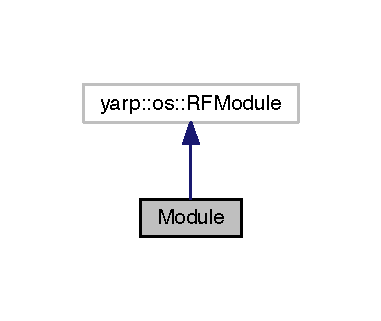
\includegraphics[width=183pt]{classModule__inherit__graph}
\end{center}
\end{figure}


Collaboration diagram for Module\+:\nopagebreak
\begin{figure}[H]
\begin{center}
\leavevmode
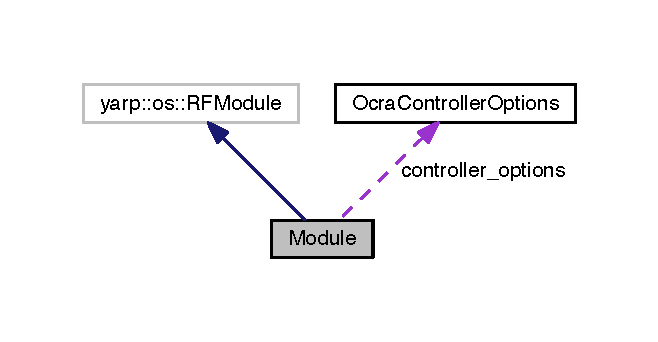
\includegraphics[width=316pt]{classModule__coll__graph}
\end{center}
\end{figure}
\subsection*{Public Member Functions}
\begin{DoxyCompactItemize}
\item 
\hyperlink{classModule_a5a240a8a9ab1813b17bcb810b24ceaea}{Module} ()
\item 
\hyperlink{classModule_a7c9d9c096786d127590fdd8aa2b7d681}{$\sim$\+Module} ()
\item 
bool \hyperlink{classModule_a1f18c762538086e1304ea18e00e51abb}{configure} (yarp\+::os\+::\+Resource\+Finder \&rf)
\item 
bool \hyperlink{classModule_ad53295be6c51e834eec92009c2d7bbf3}{interrupt\+Module} ()
\item 
bool \hyperlink{classModule_ab07583e4393148dfe0fd2ae6e7998a4b}{close} ()
\item 
bool \hyperlink{classModule_a1b1c4963512941537cef766217329a8a}{update\+Module} ()
\item 
void \hyperlink{classModule_a861f70d79b8f36dccf5daae182763bd8}{print\+Help} ()
\end{DoxyCompactItemize}
\subsection*{Private Attributes}
\begin{DoxyCompactItemize}
\item 
std\+::shared\+\_\+ptr$<$ \hyperlink{classThread}{Thread} $>$ \hyperlink{classModule_a39346aa2e2a00801e07f4c127ff004ba}{ctrl\+Thread}
\item 
std\+::shared\+\_\+ptr$<$ wbi\+::whole\+Body\+Interface $>$ \hyperlink{classModule_a0d3efedabcef6ec0db88011ccc2e7205}{robot\+Interface}
\item 
yarp\+::os\+::\+Log \hyperlink{classModule_ae029b50069bf4ff53a6f69a5bae824f6}{y\+Log}
\item 
\hyperlink{classOcraControllerOptions}{Ocra\+Controller\+Options} \hyperlink{classModule_a04156183c6e15f118595e3637ab5372f}{controller\+\_\+options}
\item 
double \hyperlink{classModule_a1a20dbf0d18e5020ad85d38a0ba22b88}{avg\+Time}
\item 
double \hyperlink{classModule_af66a2dab82208cb2ea25da22fcaaa4a3}{std\+Dev}
\item 
double \hyperlink{classModule_a5baf8260eb8a45ebbb75474f2b277edc}{avg\+Time\+Used}
\item 
double \hyperlink{classModule_a57060f2788b6dc9906e66432e775e5ac}{std\+Dev\+Used}
\item 
double \hyperlink{classModule_a33fee1e7f977b4f27a2e1488480996fb}{danger\+Period\+Loop\+Time}
\end{DoxyCompactItemize}
\subsection*{Static Private Attributes}
\begin{DoxyCompactItemize}
\item 
static const int \hyperlink{classModule_af73cdfdae53c52ea8488d0d8c4f9083f}{D\+E\+F\+A\+U\+L\+T\+\_\+\+T\+H\+R\+E\+A\+D\+\_\+\+P\+E\+R\+I\+OD} = 10
\end{DoxyCompactItemize}


\subsection{Detailed Description}
The controller module which launches the controller thread. 

Basically all this does is parse the command line arguments and look for the various config and task set files. It then instantiates a W\+BI instance (yarp\+W\+BI specifically) and a \hyperlink{classThread}{Thread} instance. It launches these threads and then basically just waits till it gets a kill (ctrl+c) command to close them down. Does a little keeping track of time as well. 

\subsection{Constructor \& Destructor Documentation}
\hypertarget{classModule_a5a240a8a9ab1813b17bcb810b24ceaea}{}\label{classModule_a5a240a8a9ab1813b17bcb810b24ceaea} 
\index{Module@{Module}!Module@{Module}}
\index{Module@{Module}!Module@{Module}}
\subsubsection{\texorpdfstring{Module()}{Module()}}
{\footnotesize\ttfamily Module\+::\+Module (\begin{DoxyParamCaption}{ }\end{DoxyParamCaption})}

Constructor which essentially does nothing. \hypertarget{classModule_a7c9d9c096786d127590fdd8aa2b7d681}{}\label{classModule_a7c9d9c096786d127590fdd8aa2b7d681} 
\index{Module@{Module}!````~Module@{$\sim$\+Module}}
\index{````~Module@{$\sim$\+Module}!Module@{Module}}
\subsubsection{\texorpdfstring{$\sim$\+Module()}{~Module()}}
{\footnotesize\ttfamily Module\+::$\sim$\+Module (\begin{DoxyParamCaption}{ }\end{DoxyParamCaption})}

Destructor which essentially does nothing. 

\subsection{Member Function Documentation}
\hypertarget{classModule_ab07583e4393148dfe0fd2ae6e7998a4b}{}\label{classModule_ab07583e4393148dfe0fd2ae6e7998a4b} 
\index{Module@{Module}!close@{close}}
\index{close@{close}!Module@{Module}}
\subsubsection{\texorpdfstring{close()}{close()}}
{\footnotesize\ttfamily bool Module\+::close (\begin{DoxyParamCaption}{ }\end{DoxyParamCaption})}

Closes the module. First shuts down the threads. \hypertarget{classModule_a1f18c762538086e1304ea18e00e51abb}{}\label{classModule_a1f18c762538086e1304ea18e00e51abb} 
\index{Module@{Module}!configure@{configure}}
\index{configure@{configure}!Module@{Module}}
\subsubsection{\texorpdfstring{configure()}{configure()}}
{\footnotesize\ttfamily bool Module\+::configure (\begin{DoxyParamCaption}\item[{yarp\+::os\+::\+Resource\+Finder \&}]{rf }\end{DoxyParamCaption})}

Configures the module by parsing the RF contents. 
\begin{DoxyParams}{Parameters}
{\em rf} & A resource finder instance which is initialized from the command line args.\\
\hline
\end{DoxyParams}
\begin{DoxyReturn}{Returns}
True or false if the configuration was successful. 
\end{DoxyReturn}
\hypertarget{classModule_ad53295be6c51e834eec92009c2d7bbf3}{}\label{classModule_ad53295be6c51e834eec92009c2d7bbf3} 
\index{Module@{Module}!interrupt\+Module@{interrupt\+Module}}
\index{interrupt\+Module@{interrupt\+Module}!Module@{Module}}
\subsubsection{\texorpdfstring{interrupt\+Module()}{interruptModule()}}
{\footnotesize\ttfamily bool Module\+::interrupt\+Module (\begin{DoxyParamCaption}{ }\end{DoxyParamCaption})}

Interrupts the module execution and stops the control and wbi threads. \hypertarget{classModule_a861f70d79b8f36dccf5daae182763bd8}{}\label{classModule_a861f70d79b8f36dccf5daae182763bd8} 
\index{Module@{Module}!print\+Help@{print\+Help}}
\index{print\+Help@{print\+Help}!Module@{Module}}
\subsubsection{\texorpdfstring{print\+Help()}{printHelp()}}
{\footnotesize\ttfamily void Module\+::print\+Help (\begin{DoxyParamCaption}{ }\end{DoxyParamCaption})}

Prints all the command line args one could use. \hypertarget{classModule_a1b1c4963512941537cef766217329a8a}{}\label{classModule_a1b1c4963512941537cef766217329a8a} 
\index{Module@{Module}!update\+Module@{update\+Module}}
\index{update\+Module@{update\+Module}!Module@{Module}}
\subsubsection{\texorpdfstring{update\+Module()}{updateModule()}}
{\footnotesize\ttfamily bool Module\+::update\+Module (\begin{DoxyParamCaption}{ }\end{DoxyParamCaption})}

Updates the \hyperlink{classModule}{Module}. Basically just clocks the thread run() method. \begin{DoxyReturn}{Returns}
Whether or not the clocking functions worked. 
\end{DoxyReturn}


\subsection{Member Data Documentation}
\hypertarget{classModule_a1a20dbf0d18e5020ad85d38a0ba22b88}{}\label{classModule_a1a20dbf0d18e5020ad85d38a0ba22b88} 
\index{Module@{Module}!avg\+Time@{avg\+Time}}
\index{avg\+Time@{avg\+Time}!Module@{Module}}
\subsubsection{\texorpdfstring{avg\+Time}{avgTime}}
{\footnotesize\ttfamily double Module\+::avg\+Time\hspace{0.3cm}{\ttfamily [private]}}

Average time between successive calls of the {\ttfamily run()} method. \hypertarget{classModule_a5baf8260eb8a45ebbb75474f2b277edc}{}\label{classModule_a5baf8260eb8a45ebbb75474f2b277edc} 
\index{Module@{Module}!avg\+Time\+Used@{avg\+Time\+Used}}
\index{avg\+Time\+Used@{avg\+Time\+Used}!Module@{Module}}
\subsubsection{\texorpdfstring{avg\+Time\+Used}{avgTimeUsed}}
{\footnotesize\ttfamily double Module\+::avg\+Time\+Used\hspace{0.3cm}{\ttfamily [private]}}

Average time for the {\ttfamily run()} method to execute. Should be close to avg\+Time. \hypertarget{classModule_a04156183c6e15f118595e3637ab5372f}{}\label{classModule_a04156183c6e15f118595e3637ab5372f} 
\index{Module@{Module}!controller\+\_\+options@{controller\+\_\+options}}
\index{controller\+\_\+options@{controller\+\_\+options}!Module@{Module}}
\subsubsection{\texorpdfstring{controller\+\_\+options}{controller\_options}}
{\footnotesize\ttfamily \hyperlink{classOcraControllerOptions}{Ocra\+Controller\+Options} Module\+::controller\+\_\+options\hspace{0.3cm}{\ttfamily [private]}}

Options used for the controller. \hypertarget{classModule_a39346aa2e2a00801e07f4c127ff004ba}{}\label{classModule_a39346aa2e2a00801e07f4c127ff004ba} 
\index{Module@{Module}!ctrl\+Thread@{ctrl\+Thread}}
\index{ctrl\+Thread@{ctrl\+Thread}!Module@{Module}}
\subsubsection{\texorpdfstring{ctrl\+Thread}{ctrlThread}}
{\footnotesize\ttfamily std\+::shared\+\_\+ptr$<$\hyperlink{classThread}{Thread}$>$ Module\+::ctrl\+Thread\hspace{0.3cm}{\ttfamily [private]}}

The controller thread. This is where the magic happens. \hypertarget{classModule_a33fee1e7f977b4f27a2e1488480996fb}{}\label{classModule_a33fee1e7f977b4f27a2e1488480996fb} 
\index{Module@{Module}!danger\+Period\+Loop\+Time@{danger\+Period\+Loop\+Time}}
\index{danger\+Period\+Loop\+Time@{danger\+Period\+Loop\+Time}!Module@{Module}}
\subsubsection{\texorpdfstring{danger\+Period\+Loop\+Time}{dangerPeriodLoopTime}}
{\footnotesize\ttfamily double Module\+::danger\+Period\+Loop\+Time\hspace{0.3cm}{\ttfamily [private]}}

A value which the thread period loop time should not exceed. \hypertarget{classModule_af73cdfdae53c52ea8488d0d8c4f9083f}{}\label{classModule_af73cdfdae53c52ea8488d0d8c4f9083f} 
\index{Module@{Module}!D\+E\+F\+A\+U\+L\+T\+\_\+\+T\+H\+R\+E\+A\+D\+\_\+\+P\+E\+R\+I\+OD@{D\+E\+F\+A\+U\+L\+T\+\_\+\+T\+H\+R\+E\+A\+D\+\_\+\+P\+E\+R\+I\+OD}}
\index{D\+E\+F\+A\+U\+L\+T\+\_\+\+T\+H\+R\+E\+A\+D\+\_\+\+P\+E\+R\+I\+OD@{D\+E\+F\+A\+U\+L\+T\+\_\+\+T\+H\+R\+E\+A\+D\+\_\+\+P\+E\+R\+I\+OD}!Module@{Module}}
\subsubsection{\texorpdfstring{D\+E\+F\+A\+U\+L\+T\+\_\+\+T\+H\+R\+E\+A\+D\+\_\+\+P\+E\+R\+I\+OD}{DEFAULT\_THREAD\_PERIOD}}
{\footnotesize\ttfamily const int Module\+::\+D\+E\+F\+A\+U\+L\+T\+\_\+\+T\+H\+R\+E\+A\+D\+\_\+\+P\+E\+R\+I\+OD = 10\hspace{0.3cm}{\ttfamily [static]}, {\ttfamily [private]}}

If the user doesn\textquotesingle{}t provide a thread period make it 10ms. \hypertarget{classModule_a0d3efedabcef6ec0db88011ccc2e7205}{}\label{classModule_a0d3efedabcef6ec0db88011ccc2e7205} 
\index{Module@{Module}!robot\+Interface@{robot\+Interface}}
\index{robot\+Interface@{robot\+Interface}!Module@{Module}}
\subsubsection{\texorpdfstring{robot\+Interface}{robotInterface}}
{\footnotesize\ttfamily std\+::shared\+\_\+ptr$<$wbi\+::whole\+Body\+Interface$>$ Module\+::robot\+Interface\hspace{0.3cm}{\ttfamily [private]}}

The yarp\+W\+BI interface used to get estimates from the robot. \hypertarget{classModule_af66a2dab82208cb2ea25da22fcaaa4a3}{}\label{classModule_af66a2dab82208cb2ea25da22fcaaa4a3} 
\index{Module@{Module}!std\+Dev@{std\+Dev}}
\index{std\+Dev@{std\+Dev}!Module@{Module}}
\subsubsection{\texorpdfstring{std\+Dev}{stdDev}}
{\footnotesize\ttfamily double Module\+::std\+Dev\hspace{0.3cm}{\ttfamily [private]}}

Standard deviation of the average time between successive calls of the {\ttfamily run()} method. \hypertarget{classModule_a57060f2788b6dc9906e66432e775e5ac}{}\label{classModule_a57060f2788b6dc9906e66432e775e5ac} 
\index{Module@{Module}!std\+Dev\+Used@{std\+Dev\+Used}}
\index{std\+Dev\+Used@{std\+Dev\+Used}!Module@{Module}}
\subsubsection{\texorpdfstring{std\+Dev\+Used}{stdDevUsed}}
{\footnotesize\ttfamily double Module\+::std\+Dev\+Used\hspace{0.3cm}{\ttfamily [private]}}

Standard deviation of the average time for the {\ttfamily run()} method to execute. \hypertarget{classModule_ae029b50069bf4ff53a6f69a5bae824f6}{}\label{classModule_ae029b50069bf4ff53a6f69a5bae824f6} 
\index{Module@{Module}!y\+Log@{y\+Log}}
\index{y\+Log@{y\+Log}!Module@{Module}}
\subsubsection{\texorpdfstring{y\+Log}{yLog}}
{\footnotesize\ttfamily yarp\+::os\+::\+Log Module\+::y\+Log\hspace{0.3cm}{\ttfamily [private]}}

A yarp logging tool. 

The documentation for this class was generated from the following files\+:\begin{DoxyCompactItemize}
\item 
/\+Users/jorhabibeljaik/\+Code/codyco-\/superbuild/main/ocra-\/wbi-\/plugins/ocra-\/icub-\/server/include/ocra-\/icub-\/server/\hyperlink{Module_8h}{Module.\+h}\item 
/\+Users/jorhabibeljaik/\+Code/codyco-\/superbuild/main/ocra-\/wbi-\/plugins/ocra-\/icub-\/server/src/\hyperlink{Module_8cpp}{Module.\+cpp}\end{DoxyCompactItemize}

\hypertarget{classOcraControllerOptions}{}\section{Ocra\+Controller\+Options Class Reference}
\label{classOcraControllerOptions}\index{Ocra\+Controller\+Options@{Ocra\+Controller\+Options}}


{\ttfamily \#include $<$Thread.\+h$>$}

\subsection*{Public Member Functions}
\begin{DoxyCompactItemize}
\item 
\hyperlink{classOcraControllerOptions_a1a91de992c42c6da488e95cd594eca80}{Ocra\+Controller\+Options} ()
\item 
\hyperlink{classOcraControllerOptions_a22f514e92ccf91cc362c48a6c340ac19}{$\sim$\+Ocra\+Controller\+Options} ()
\end{DoxyCompactItemize}
\subsection*{Public Attributes}
\begin{DoxyCompactItemize}
\item 
int \hyperlink{classOcraControllerOptions_ab706ae593bf5b30433cfd6f957b51db4}{thread\+Period}
\item 
std\+::string \hyperlink{classOcraControllerOptions_a22380b083fbf0b202993d0415d1d4c83}{server\+Name}
\item 
std\+::string \hyperlink{classOcraControllerOptions_a897948011f23b08ba20e1707033458d4}{robot\+Name}
\item 
std\+::string \hyperlink{classOcraControllerOptions_af91566ecff3f7ed02571369c7af061ce}{startup\+Task\+Set\+Path}
\item 
std\+::string \hyperlink{classOcraControllerOptions_ab01efbd786ad8bc5beb6de02dbcd0936}{startup\+Sequence}
\item 
std\+::string \hyperlink{classOcraControllerOptions_af3a98210531cf667c2838e45b470a66e}{wbi\+Config\+File\+Path}
\item 
std\+::string \hyperlink{classOcraControllerOptions_a697196e6267b2a519dd0bcc2bc03ab73}{urdf\+Model\+Path}
\item 
bool \hyperlink{classOcraControllerOptions_a26dce90c0e6cf7ba608020d01cd08f3c}{run\+In\+Debug\+Mode}
\item 
bool \hyperlink{classOcraControllerOptions_a1edf322553d88c1ac2bf8947e9d942d7}{is\+Floating\+Base}
\item 
bool \hyperlink{classOcraControllerOptions_a335f09b446b6d10e2a8e6eb453391d9e}{use\+Odometry}
\item 
yarp\+::os\+::\+Property \hyperlink{classOcraControllerOptions_ac3965bdcce6cb2ce3e4a335f855acd63}{yarp\+Wbi\+Options}
\item 
ocra\+\_\+recipes\+::\+C\+O\+N\+T\+R\+O\+L\+L\+E\+R\+\_\+\+T\+Y\+PE \hyperlink{classOcraControllerOptions_aa533fe11c53b7fb17105f1edf48e1c0d}{controller\+Type}
\item 
ocra\+\_\+recipes\+::\+S\+O\+L\+V\+E\+R\+\_\+\+T\+Y\+PE \hyperlink{classOcraControllerOptions_af79b8705c3f3097b642262bc877eaa8e}{solver}
\end{DoxyCompactItemize}


\subsection{Constructor \& Destructor Documentation}
\hypertarget{classOcraControllerOptions_a1a91de992c42c6da488e95cd594eca80}{}\label{classOcraControllerOptions_a1a91de992c42c6da488e95cd594eca80} 
\index{Ocra\+Controller\+Options@{Ocra\+Controller\+Options}!Ocra\+Controller\+Options@{Ocra\+Controller\+Options}}
\index{Ocra\+Controller\+Options@{Ocra\+Controller\+Options}!Ocra\+Controller\+Options@{Ocra\+Controller\+Options}}
\subsubsection{\texorpdfstring{Ocra\+Controller\+Options()}{OcraControllerOptions()}}
{\footnotesize\ttfamily Ocra\+Controller\+Options\+::\+Ocra\+Controller\+Options (\begin{DoxyParamCaption}{ }\end{DoxyParamCaption})}

Constructor. Initializes all of the possible values. \hypertarget{classOcraControllerOptions_a22f514e92ccf91cc362c48a6c340ac19}{}\label{classOcraControllerOptions_a22f514e92ccf91cc362c48a6c340ac19} 
\index{Ocra\+Controller\+Options@{Ocra\+Controller\+Options}!````~Ocra\+Controller\+Options@{$\sim$\+Ocra\+Controller\+Options}}
\index{````~Ocra\+Controller\+Options@{$\sim$\+Ocra\+Controller\+Options}!Ocra\+Controller\+Options@{Ocra\+Controller\+Options}}
\subsubsection{\texorpdfstring{$\sim$\+Ocra\+Controller\+Options()}{~OcraControllerOptions()}}
{\footnotesize\ttfamily Ocra\+Controller\+Options\+::$\sim$\+Ocra\+Controller\+Options (\begin{DoxyParamCaption}{ }\end{DoxyParamCaption})}

Destructor. Does nothing. 

\subsection{Member Data Documentation}
\hypertarget{classOcraControllerOptions_aa533fe11c53b7fb17105f1edf48e1c0d}{}\label{classOcraControllerOptions_aa533fe11c53b7fb17105f1edf48e1c0d} 
\index{Ocra\+Controller\+Options@{Ocra\+Controller\+Options}!controller\+Type@{controller\+Type}}
\index{controller\+Type@{controller\+Type}!Ocra\+Controller\+Options@{Ocra\+Controller\+Options}}
\subsubsection{\texorpdfstring{controller\+Type}{controllerType}}
{\footnotesize\ttfamily ocra\+\_\+recipes\+::\+C\+O\+N\+T\+R\+O\+L\+L\+E\+R\+\_\+\+T\+Y\+PE Ocra\+Controller\+Options\+::controller\+Type}

The type of O\+C\+RA controller to use. \hypertarget{classOcraControllerOptions_a1edf322553d88c1ac2bf8947e9d942d7}{}\label{classOcraControllerOptions_a1edf322553d88c1ac2bf8947e9d942d7} 
\index{Ocra\+Controller\+Options@{Ocra\+Controller\+Options}!is\+Floating\+Base@{is\+Floating\+Base}}
\index{is\+Floating\+Base@{is\+Floating\+Base}!Ocra\+Controller\+Options@{Ocra\+Controller\+Options}}
\subsubsection{\texorpdfstring{is\+Floating\+Base}{isFloatingBase}}
{\footnotesize\ttfamily bool Ocra\+Controller\+Options\+::is\+Floating\+Base}

a boolean which tells the controller whether the robot has a fixed or floating base. \hypertarget{classOcraControllerOptions_a897948011f23b08ba20e1707033458d4}{}\label{classOcraControllerOptions_a897948011f23b08ba20e1707033458d4} 
\index{Ocra\+Controller\+Options@{Ocra\+Controller\+Options}!robot\+Name@{robot\+Name}}
\index{robot\+Name@{robot\+Name}!Ocra\+Controller\+Options@{Ocra\+Controller\+Options}}
\subsubsection{\texorpdfstring{robot\+Name}{robotName}}
{\footnotesize\ttfamily std\+::string Ocra\+Controller\+Options\+::robot\+Name}

a string with the name of the robot. \hypertarget{classOcraControllerOptions_a26dce90c0e6cf7ba608020d01cd08f3c}{}\label{classOcraControllerOptions_a26dce90c0e6cf7ba608020d01cd08f3c} 
\index{Ocra\+Controller\+Options@{Ocra\+Controller\+Options}!run\+In\+Debug\+Mode@{run\+In\+Debug\+Mode}}
\index{run\+In\+Debug\+Mode@{run\+In\+Debug\+Mode}!Ocra\+Controller\+Options@{Ocra\+Controller\+Options}}
\subsubsection{\texorpdfstring{run\+In\+Debug\+Mode}{runInDebugMode}}
{\footnotesize\ttfamily bool Ocra\+Controller\+Options\+::run\+In\+Debug\+Mode}

a boolean which runs the controller in a debugging mode which allows one to check the controller ouput joint by joint. \hypertarget{classOcraControllerOptions_a22380b083fbf0b202993d0415d1d4c83}{}\label{classOcraControllerOptions_a22380b083fbf0b202993d0415d1d4c83} 
\index{Ocra\+Controller\+Options@{Ocra\+Controller\+Options}!server\+Name@{server\+Name}}
\index{server\+Name@{server\+Name}!Ocra\+Controller\+Options@{Ocra\+Controller\+Options}}
\subsubsection{\texorpdfstring{server\+Name}{serverName}}
{\footnotesize\ttfamily std\+::string Ocra\+Controller\+Options\+::server\+Name}

a string with the name of the controller server. \hypertarget{classOcraControllerOptions_af79b8705c3f3097b642262bc877eaa8e}{}\label{classOcraControllerOptions_af79b8705c3f3097b642262bc877eaa8e} 
\index{Ocra\+Controller\+Options@{Ocra\+Controller\+Options}!solver@{solver}}
\index{solver@{solver}!Ocra\+Controller\+Options@{Ocra\+Controller\+Options}}
\subsubsection{\texorpdfstring{solver}{solver}}
{\footnotesize\ttfamily ocra\+\_\+recipes\+::\+S\+O\+L\+V\+E\+R\+\_\+\+T\+Y\+PE Ocra\+Controller\+Options\+::solver}

The type of O\+C\+RA controller to use. \hypertarget{classOcraControllerOptions_ab01efbd786ad8bc5beb6de02dbcd0936}{}\label{classOcraControllerOptions_ab01efbd786ad8bc5beb6de02dbcd0936} 
\index{Ocra\+Controller\+Options@{Ocra\+Controller\+Options}!startup\+Sequence@{startup\+Sequence}}
\index{startup\+Sequence@{startup\+Sequence}!Ocra\+Controller\+Options@{Ocra\+Controller\+Options}}
\subsubsection{\texorpdfstring{startup\+Sequence}{startupSequence}}
{\footnotesize\ttfamily std\+::string Ocra\+Controller\+Options\+::startup\+Sequence}

a string with the name of a sequence to run $\ast$$\ast$(will be removed)$\ast$$\ast$. \hypertarget{classOcraControllerOptions_af91566ecff3f7ed02571369c7af061ce}{}\label{classOcraControllerOptions_af91566ecff3f7ed02571369c7af061ce} 
\index{Ocra\+Controller\+Options@{Ocra\+Controller\+Options}!startup\+Task\+Set\+Path@{startup\+Task\+Set\+Path}}
\index{startup\+Task\+Set\+Path@{startup\+Task\+Set\+Path}!Ocra\+Controller\+Options@{Ocra\+Controller\+Options}}
\subsubsection{\texorpdfstring{startup\+Task\+Set\+Path}{startupTaskSetPath}}
{\footnotesize\ttfamily std\+::string Ocra\+Controller\+Options\+::startup\+Task\+Set\+Path}

a string with the absolute path to an xml file with a set of tasks. \hypertarget{classOcraControllerOptions_ab706ae593bf5b30433cfd6f957b51db4}{}\label{classOcraControllerOptions_ab706ae593bf5b30433cfd6f957b51db4} 
\index{Ocra\+Controller\+Options@{Ocra\+Controller\+Options}!thread\+Period@{thread\+Period}}
\index{thread\+Period@{thread\+Period}!Ocra\+Controller\+Options@{Ocra\+Controller\+Options}}
\subsubsection{\texorpdfstring{thread\+Period}{threadPeriod}}
{\footnotesize\ttfamily int Ocra\+Controller\+Options\+::thread\+Period}

An int representing the looping period of the controller. \hypertarget{classOcraControllerOptions_a697196e6267b2a519dd0bcc2bc03ab73}{}\label{classOcraControllerOptions_a697196e6267b2a519dd0bcc2bc03ab73} 
\index{Ocra\+Controller\+Options@{Ocra\+Controller\+Options}!urdf\+Model\+Path@{urdf\+Model\+Path}}
\index{urdf\+Model\+Path@{urdf\+Model\+Path}!Ocra\+Controller\+Options@{Ocra\+Controller\+Options}}
\subsubsection{\texorpdfstring{urdf\+Model\+Path}{urdfModelPath}}
{\footnotesize\ttfamily std\+::string Ocra\+Controller\+Options\+::urdf\+Model\+Path}

Absolute path to the urdf model. Used for the odometry. \hypertarget{classOcraControllerOptions_a335f09b446b6d10e2a8e6eb453391d9e}{}\label{classOcraControllerOptions_a335f09b446b6d10e2a8e6eb453391d9e} 
\index{Ocra\+Controller\+Options@{Ocra\+Controller\+Options}!use\+Odometry@{use\+Odometry}}
\index{use\+Odometry@{use\+Odometry}!Ocra\+Controller\+Options@{Ocra\+Controller\+Options}}
\subsubsection{\texorpdfstring{use\+Odometry}{useOdometry}}
{\footnotesize\ttfamily bool Ocra\+Controller\+Options\+::use\+Odometry}

a boolean which tells the controller to start the odometry, meaning that the world reference frame remains attached to the ground \hypertarget{classOcraControllerOptions_af3a98210531cf667c2838e45b470a66e}{}\label{classOcraControllerOptions_af3a98210531cf667c2838e45b470a66e} 
\index{Ocra\+Controller\+Options@{Ocra\+Controller\+Options}!wbi\+Config\+File\+Path@{wbi\+Config\+File\+Path}}
\index{wbi\+Config\+File\+Path@{wbi\+Config\+File\+Path}!Ocra\+Controller\+Options@{Ocra\+Controller\+Options}}
\subsubsection{\texorpdfstring{wbi\+Config\+File\+Path}{wbiConfigFilePath}}
{\footnotesize\ttfamily std\+::string Ocra\+Controller\+Options\+::wbi\+Config\+File\+Path}

The absolute path to the configuration file used to initialize the yarp\+W\+BI. \hypertarget{classOcraControllerOptions_ac3965bdcce6cb2ce3e4a335f855acd63}{}\label{classOcraControllerOptions_ac3965bdcce6cb2ce3e4a335f855acd63} 
\index{Ocra\+Controller\+Options@{Ocra\+Controller\+Options}!yarp\+Wbi\+Options@{yarp\+Wbi\+Options}}
\index{yarp\+Wbi\+Options@{yarp\+Wbi\+Options}!Ocra\+Controller\+Options@{Ocra\+Controller\+Options}}
\subsubsection{\texorpdfstring{yarp\+Wbi\+Options}{yarpWbiOptions}}
{\footnotesize\ttfamily yarp\+::os\+::\+Property Ocra\+Controller\+Options\+::yarp\+Wbi\+Options}

Options for the W\+BI used to update the model. 

The documentation for this class was generated from the following files\+:\begin{DoxyCompactItemize}
\item 
/\+Users/jorhabibeljaik/\+Code/codyco-\/superbuild/main/ocra-\/wbi-\/plugins/ocra-\/icub-\/server/include/ocra-\/icub-\/server/\hyperlink{Thread_8h}{Thread.\+h}\item 
/\+Users/jorhabibeljaik/\+Code/codyco-\/superbuild/main/ocra-\/wbi-\/plugins/ocra-\/icub-\/server/src/\hyperlink{Thread_8cpp}{Thread.\+cpp}\end{DoxyCompactItemize}

\hypertarget{classocra__icub_1_1OcraWbiConversions}{}\section{ocra\+\_\+icub\+:\+:Ocra\+Wbi\+Conversions Class Reference}
\label{classocra__icub_1_1OcraWbiConversions}\index{ocra\+\_\+icub\+::\+Ocra\+Wbi\+Conversions@{ocra\+\_\+icub\+::\+Ocra\+Wbi\+Conversions}}


{\ttfamily \#include $<$Ocra\+Wbi\+Conversions.\+h$>$}

\subsection*{Static Public Member Functions}
\begin{DoxyCompactItemize}
\item 
static bool \hyperlink{classocra__icub_1_1OcraWbiConversions_af71562a5f3d4f6e649f1cec0a3d9996b}{eigen\+Dispd\+To\+Wbi\+Frame} (const Eigen\+::\+Displacementd \&disp, wbi\+::\+Frame \&frame)
\item 
static bool \hyperlink{classocra__icub_1_1OcraWbiConversions_a403627efa183c8ddbbccabf0dcd5bcaf}{wbi\+Frame\+To\+Eigen\+Dispd} (const wbi\+::\+Frame \&frame, Eigen\+::\+Displacementd \&disp)
\item 
static bool \hyperlink{classocra__icub_1_1OcraWbiConversions_a37c2aea3bf156928cb90a16655c24cc9}{wbi\+To\+Ocra\+Twist\+Vector} (Eigen\+::\+Twistd \&t\+\_\+wbi, Eigen\+::\+Twistd \&t\+\_\+ocra)
\item 
static bool \hyperlink{classocra__icub_1_1OcraWbiConversions_a7725aea95eb71c805def4a064a2693fa}{ocra\+To\+Wbi\+Twist\+Vector} (Eigen\+::\+Twistd \&t\+\_\+ocra, Eigen\+::\+Twistd \&t\+\_\+wbi)
\item 
static bool \hyperlink{classocra__icub_1_1OcraWbiConversions_a25a64172ebb14db9ddf301880a433964}{wbi\+To\+Ocra\+Seg\+Jacobian} (const Eigen\+::\+Matrix\+Xd \&jac, Eigen\+::\+Matrix\+Xd \&J)
\item 
static bool \hyperlink{classocra__icub_1_1OcraWbiConversions_a86458de950caa3bde3aa1d1aff448be1}{wbi\+To\+Ocra\+Co\+M\+Jacobian} (const Eigen\+::\+Matrix\+Xd \&jac, Eigen\+::\+Matrix$<$ double, 3, Eigen\+::\+Dynamic $>$ \&J)
\item 
static bool \hyperlink{classocra__icub_1_1OcraWbiConversions_ac03ed9581c49479b3ade94d58a3295b4}{eigen\+Row\+Major\+To\+Col\+Major} (const \hyperlink{namespaceocra__icub_aa5e36a19ed031c28ca83c207bd7dd83f}{Matrix\+Xd\+Rm} \&M\+\_\+rm, Eigen\+::\+Matrix\+Xd \&M)
\item 
static bool \hyperlink{classocra__icub_1_1OcraWbiConversions_abaa2b7a9069b60cfb36cb21e89b98177}{wbi\+To\+Ocra\+Mass\+Matrix} (int qdof, const Eigen\+::\+Matrix\+Xd \&M\+\_\+wbi, Eigen\+::\+Matrix\+Xd \&M\+\_\+ocra)
\item 
static bool \hyperlink{classocra__icub_1_1OcraWbiConversions_ae8839dfdc97e2239f4ed8a257d32fb21}{wbi\+To\+Ocra\+Body\+Vector} (int qdof, const Eigen\+::\+Vector\+Xd \&v\+\_\+wbi, Eigen\+::\+Vector\+Xd \&v\+\_\+ocra)
\item 
static bool \hyperlink{classocra__icub_1_1OcraWbiConversions_a1197be5b35329fbec85de8ee3c4abbd5}{eigen\+To\+Yarp\+Vector} (const Eigen\+::\+Vector\+Xd \&eigen\+Vector, yarp\+::sig\+::\+Vector \&yarp\+Vector)
\end{DoxyCompactItemize}
\subsection*{Static Public Attributes}
\begin{DoxyCompactItemize}
\item 
static const int \hyperlink{classocra__icub_1_1OcraWbiConversions_a7c628bd1208c5e70be458d4dffda4d06}{D\+I\+M\+\_\+\+T\+R\+A\+N\+S\+L\+A\+T\+I\+ON} = 3
\item 
static const int \hyperlink{classocra__icub_1_1OcraWbiConversions_a05e66392df58e9dda2d4db590bdd65a0}{D\+I\+M\+\_\+\+R\+O\+T\+A\+T\+I\+ON} = 3
\end{DoxyCompactItemize}


\subsection{Member Function Documentation}
\hypertarget{classocra__icub_1_1OcraWbiConversions_af71562a5f3d4f6e649f1cec0a3d9996b}{}\label{classocra__icub_1_1OcraWbiConversions_af71562a5f3d4f6e649f1cec0a3d9996b} 
\index{ocra\+\_\+icub\+::\+Ocra\+Wbi\+Conversions@{ocra\+\_\+icub\+::\+Ocra\+Wbi\+Conversions}!eigen\+Dispd\+To\+Wbi\+Frame@{eigen\+Dispd\+To\+Wbi\+Frame}}
\index{eigen\+Dispd\+To\+Wbi\+Frame@{eigen\+Dispd\+To\+Wbi\+Frame}!ocra\+\_\+icub\+::\+Ocra\+Wbi\+Conversions@{ocra\+\_\+icub\+::\+Ocra\+Wbi\+Conversions}}
\subsubsection{\texorpdfstring{eigen\+Dispd\+To\+Wbi\+Frame()}{eigenDispdToWbiFrame()}}
{\footnotesize\ttfamily bool Ocra\+Wbi\+Conversions\+::eigen\+Dispd\+To\+Wbi\+Frame (\begin{DoxyParamCaption}\item[{const Eigen\+::\+Displacementd \&}]{disp,  }\item[{wbi\+::\+Frame \&}]{frame }\end{DoxyParamCaption})\hspace{0.3cm}{\ttfamily [static]}}

\hypertarget{classocra__icub_1_1OcraWbiConversions_ac03ed9581c49479b3ade94d58a3295b4}{}\label{classocra__icub_1_1OcraWbiConversions_ac03ed9581c49479b3ade94d58a3295b4} 
\index{ocra\+\_\+icub\+::\+Ocra\+Wbi\+Conversions@{ocra\+\_\+icub\+::\+Ocra\+Wbi\+Conversions}!eigen\+Row\+Major\+To\+Col\+Major@{eigen\+Row\+Major\+To\+Col\+Major}}
\index{eigen\+Row\+Major\+To\+Col\+Major@{eigen\+Row\+Major\+To\+Col\+Major}!ocra\+\_\+icub\+::\+Ocra\+Wbi\+Conversions@{ocra\+\_\+icub\+::\+Ocra\+Wbi\+Conversions}}
\subsubsection{\texorpdfstring{eigen\+Row\+Major\+To\+Col\+Major()}{eigenRowMajorToColMajor()}}
{\footnotesize\ttfamily bool Ocra\+Wbi\+Conversions\+::eigen\+Row\+Major\+To\+Col\+Major (\begin{DoxyParamCaption}\item[{const \hyperlink{namespaceocra__icub_aa5e36a19ed031c28ca83c207bd7dd83f}{Matrix\+Xd\+Rm} \&}]{M\+\_\+rm,  }\item[{Eigen\+::\+Matrix\+Xd \&}]{M }\end{DoxyParamCaption})\hspace{0.3cm}{\ttfamily [static]}}

\hypertarget{classocra__icub_1_1OcraWbiConversions_a1197be5b35329fbec85de8ee3c4abbd5}{}\label{classocra__icub_1_1OcraWbiConversions_a1197be5b35329fbec85de8ee3c4abbd5} 
\index{ocra\+\_\+icub\+::\+Ocra\+Wbi\+Conversions@{ocra\+\_\+icub\+::\+Ocra\+Wbi\+Conversions}!eigen\+To\+Yarp\+Vector@{eigen\+To\+Yarp\+Vector}}
\index{eigen\+To\+Yarp\+Vector@{eigen\+To\+Yarp\+Vector}!ocra\+\_\+icub\+::\+Ocra\+Wbi\+Conversions@{ocra\+\_\+icub\+::\+Ocra\+Wbi\+Conversions}}
\subsubsection{\texorpdfstring{eigen\+To\+Yarp\+Vector()}{eigenToYarpVector()}}
{\footnotesize\ttfamily bool Ocra\+Wbi\+Conversions\+::eigen\+To\+Yarp\+Vector (\begin{DoxyParamCaption}\item[{const Eigen\+::\+Vector\+Xd \&}]{eigen\+Vector,  }\item[{yarp\+::sig\+::\+Vector \&}]{yarp\+Vector }\end{DoxyParamCaption})\hspace{0.3cm}{\ttfamily [static]}}

\hypertarget{classocra__icub_1_1OcraWbiConversions_a7725aea95eb71c805def4a064a2693fa}{}\label{classocra__icub_1_1OcraWbiConversions_a7725aea95eb71c805def4a064a2693fa} 
\index{ocra\+\_\+icub\+::\+Ocra\+Wbi\+Conversions@{ocra\+\_\+icub\+::\+Ocra\+Wbi\+Conversions}!ocra\+To\+Wbi\+Twist\+Vector@{ocra\+To\+Wbi\+Twist\+Vector}}
\index{ocra\+To\+Wbi\+Twist\+Vector@{ocra\+To\+Wbi\+Twist\+Vector}!ocra\+\_\+icub\+::\+Ocra\+Wbi\+Conversions@{ocra\+\_\+icub\+::\+Ocra\+Wbi\+Conversions}}
\subsubsection{\texorpdfstring{ocra\+To\+Wbi\+Twist\+Vector()}{ocraToWbiTwistVector()}}
{\footnotesize\ttfamily bool Ocra\+Wbi\+Conversions\+::ocra\+To\+Wbi\+Twist\+Vector (\begin{DoxyParamCaption}\item[{Eigen\+::\+Twistd \&}]{t\+\_\+ocra,  }\item[{Eigen\+::\+Twistd \&}]{t\+\_\+wbi }\end{DoxyParamCaption})\hspace{0.3cm}{\ttfamily [static]}}

\hypertarget{classocra__icub_1_1OcraWbiConversions_a403627efa183c8ddbbccabf0dcd5bcaf}{}\label{classocra__icub_1_1OcraWbiConversions_a403627efa183c8ddbbccabf0dcd5bcaf} 
\index{ocra\+\_\+icub\+::\+Ocra\+Wbi\+Conversions@{ocra\+\_\+icub\+::\+Ocra\+Wbi\+Conversions}!wbi\+Frame\+To\+Eigen\+Dispd@{wbi\+Frame\+To\+Eigen\+Dispd}}
\index{wbi\+Frame\+To\+Eigen\+Dispd@{wbi\+Frame\+To\+Eigen\+Dispd}!ocra\+\_\+icub\+::\+Ocra\+Wbi\+Conversions@{ocra\+\_\+icub\+::\+Ocra\+Wbi\+Conversions}}
\subsubsection{\texorpdfstring{wbi\+Frame\+To\+Eigen\+Dispd()}{wbiFrameToEigenDispd()}}
{\footnotesize\ttfamily bool Ocra\+Wbi\+Conversions\+::wbi\+Frame\+To\+Eigen\+Dispd (\begin{DoxyParamCaption}\item[{const wbi\+::\+Frame \&}]{frame,  }\item[{Eigen\+::\+Displacementd \&}]{disp }\end{DoxyParamCaption})\hspace{0.3cm}{\ttfamily [static]}}

\hypertarget{classocra__icub_1_1OcraWbiConversions_ae8839dfdc97e2239f4ed8a257d32fb21}{}\label{classocra__icub_1_1OcraWbiConversions_ae8839dfdc97e2239f4ed8a257d32fb21} 
\index{ocra\+\_\+icub\+::\+Ocra\+Wbi\+Conversions@{ocra\+\_\+icub\+::\+Ocra\+Wbi\+Conversions}!wbi\+To\+Ocra\+Body\+Vector@{wbi\+To\+Ocra\+Body\+Vector}}
\index{wbi\+To\+Ocra\+Body\+Vector@{wbi\+To\+Ocra\+Body\+Vector}!ocra\+\_\+icub\+::\+Ocra\+Wbi\+Conversions@{ocra\+\_\+icub\+::\+Ocra\+Wbi\+Conversions}}
\subsubsection{\texorpdfstring{wbi\+To\+Ocra\+Body\+Vector()}{wbiToOcraBodyVector()}}
{\footnotesize\ttfamily bool Ocra\+Wbi\+Conversions\+::wbi\+To\+Ocra\+Body\+Vector (\begin{DoxyParamCaption}\item[{int}]{qdof,  }\item[{const Eigen\+::\+Vector\+Xd \&}]{v\+\_\+wbi,  }\item[{Eigen\+::\+Vector\+Xd \&}]{v\+\_\+ocra }\end{DoxyParamCaption})\hspace{0.3cm}{\ttfamily [static]}}

\hypertarget{classocra__icub_1_1OcraWbiConversions_a86458de950caa3bde3aa1d1aff448be1}{}\label{classocra__icub_1_1OcraWbiConversions_a86458de950caa3bde3aa1d1aff448be1} 
\index{ocra\+\_\+icub\+::\+Ocra\+Wbi\+Conversions@{ocra\+\_\+icub\+::\+Ocra\+Wbi\+Conversions}!wbi\+To\+Ocra\+Co\+M\+Jacobian@{wbi\+To\+Ocra\+Co\+M\+Jacobian}}
\index{wbi\+To\+Ocra\+Co\+M\+Jacobian@{wbi\+To\+Ocra\+Co\+M\+Jacobian}!ocra\+\_\+icub\+::\+Ocra\+Wbi\+Conversions@{ocra\+\_\+icub\+::\+Ocra\+Wbi\+Conversions}}
\subsubsection{\texorpdfstring{wbi\+To\+Ocra\+Co\+M\+Jacobian()}{wbiToOcraCoMJacobian()}}
{\footnotesize\ttfamily bool Ocra\+Wbi\+Conversions\+::wbi\+To\+Ocra\+Co\+M\+Jacobian (\begin{DoxyParamCaption}\item[{const Eigen\+::\+Matrix\+Xd \&}]{jac,  }\item[{Eigen\+::\+Matrix$<$ double, 3, Eigen\+::\+Dynamic $>$ \&}]{J }\end{DoxyParamCaption})\hspace{0.3cm}{\ttfamily [static]}}

\hypertarget{classocra__icub_1_1OcraWbiConversions_abaa2b7a9069b60cfb36cb21e89b98177}{}\label{classocra__icub_1_1OcraWbiConversions_abaa2b7a9069b60cfb36cb21e89b98177} 
\index{ocra\+\_\+icub\+::\+Ocra\+Wbi\+Conversions@{ocra\+\_\+icub\+::\+Ocra\+Wbi\+Conversions}!wbi\+To\+Ocra\+Mass\+Matrix@{wbi\+To\+Ocra\+Mass\+Matrix}}
\index{wbi\+To\+Ocra\+Mass\+Matrix@{wbi\+To\+Ocra\+Mass\+Matrix}!ocra\+\_\+icub\+::\+Ocra\+Wbi\+Conversions@{ocra\+\_\+icub\+::\+Ocra\+Wbi\+Conversions}}
\subsubsection{\texorpdfstring{wbi\+To\+Ocra\+Mass\+Matrix()}{wbiToOcraMassMatrix()}}
{\footnotesize\ttfamily bool Ocra\+Wbi\+Conversions\+::wbi\+To\+Ocra\+Mass\+Matrix (\begin{DoxyParamCaption}\item[{int}]{qdof,  }\item[{const Eigen\+::\+Matrix\+Xd \&}]{M\+\_\+wbi,  }\item[{Eigen\+::\+Matrix\+Xd \&}]{M\+\_\+ocra }\end{DoxyParamCaption})\hspace{0.3cm}{\ttfamily [static]}}

\hypertarget{classocra__icub_1_1OcraWbiConversions_a25a64172ebb14db9ddf301880a433964}{}\label{classocra__icub_1_1OcraWbiConversions_a25a64172ebb14db9ddf301880a433964} 
\index{ocra\+\_\+icub\+::\+Ocra\+Wbi\+Conversions@{ocra\+\_\+icub\+::\+Ocra\+Wbi\+Conversions}!wbi\+To\+Ocra\+Seg\+Jacobian@{wbi\+To\+Ocra\+Seg\+Jacobian}}
\index{wbi\+To\+Ocra\+Seg\+Jacobian@{wbi\+To\+Ocra\+Seg\+Jacobian}!ocra\+\_\+icub\+::\+Ocra\+Wbi\+Conversions@{ocra\+\_\+icub\+::\+Ocra\+Wbi\+Conversions}}
\subsubsection{\texorpdfstring{wbi\+To\+Ocra\+Seg\+Jacobian()}{wbiToOcraSegJacobian()}}
{\footnotesize\ttfamily bool Ocra\+Wbi\+Conversions\+::wbi\+To\+Ocra\+Seg\+Jacobian (\begin{DoxyParamCaption}\item[{const Eigen\+::\+Matrix\+Xd \&}]{jac,  }\item[{Eigen\+::\+Matrix\+Xd \&}]{J }\end{DoxyParamCaption})\hspace{0.3cm}{\ttfamily [static]}}

\hypertarget{classocra__icub_1_1OcraWbiConversions_a37c2aea3bf156928cb90a16655c24cc9}{}\label{classocra__icub_1_1OcraWbiConversions_a37c2aea3bf156928cb90a16655c24cc9} 
\index{ocra\+\_\+icub\+::\+Ocra\+Wbi\+Conversions@{ocra\+\_\+icub\+::\+Ocra\+Wbi\+Conversions}!wbi\+To\+Ocra\+Twist\+Vector@{wbi\+To\+Ocra\+Twist\+Vector}}
\index{wbi\+To\+Ocra\+Twist\+Vector@{wbi\+To\+Ocra\+Twist\+Vector}!ocra\+\_\+icub\+::\+Ocra\+Wbi\+Conversions@{ocra\+\_\+icub\+::\+Ocra\+Wbi\+Conversions}}
\subsubsection{\texorpdfstring{wbi\+To\+Ocra\+Twist\+Vector()}{wbiToOcraTwistVector()}}
{\footnotesize\ttfamily bool Ocra\+Wbi\+Conversions\+::wbi\+To\+Ocra\+Twist\+Vector (\begin{DoxyParamCaption}\item[{Eigen\+::\+Twistd \&}]{t\+\_\+wbi,  }\item[{Eigen\+::\+Twistd \&}]{t\+\_\+ocra }\end{DoxyParamCaption})\hspace{0.3cm}{\ttfamily [static]}}



\subsection{Member Data Documentation}
\hypertarget{classocra__icub_1_1OcraWbiConversions_a05e66392df58e9dda2d4db590bdd65a0}{}\label{classocra__icub_1_1OcraWbiConversions_a05e66392df58e9dda2d4db590bdd65a0} 
\index{ocra\+\_\+icub\+::\+Ocra\+Wbi\+Conversions@{ocra\+\_\+icub\+::\+Ocra\+Wbi\+Conversions}!D\+I\+M\+\_\+\+R\+O\+T\+A\+T\+I\+ON@{D\+I\+M\+\_\+\+R\+O\+T\+A\+T\+I\+ON}}
\index{D\+I\+M\+\_\+\+R\+O\+T\+A\+T\+I\+ON@{D\+I\+M\+\_\+\+R\+O\+T\+A\+T\+I\+ON}!ocra\+\_\+icub\+::\+Ocra\+Wbi\+Conversions@{ocra\+\_\+icub\+::\+Ocra\+Wbi\+Conversions}}
\subsubsection{\texorpdfstring{D\+I\+M\+\_\+\+R\+O\+T\+A\+T\+I\+ON}{DIM\_ROTATION}}
{\footnotesize\ttfamily const int ocra\+\_\+icub\+::\+Ocra\+Wbi\+Conversions\+::\+D\+I\+M\+\_\+\+R\+O\+T\+A\+T\+I\+ON = 3\hspace{0.3cm}{\ttfamily [static]}}

\hypertarget{classocra__icub_1_1OcraWbiConversions_a7c628bd1208c5e70be458d4dffda4d06}{}\label{classocra__icub_1_1OcraWbiConversions_a7c628bd1208c5e70be458d4dffda4d06} 
\index{ocra\+\_\+icub\+::\+Ocra\+Wbi\+Conversions@{ocra\+\_\+icub\+::\+Ocra\+Wbi\+Conversions}!D\+I\+M\+\_\+\+T\+R\+A\+N\+S\+L\+A\+T\+I\+ON@{D\+I\+M\+\_\+\+T\+R\+A\+N\+S\+L\+A\+T\+I\+ON}}
\index{D\+I\+M\+\_\+\+T\+R\+A\+N\+S\+L\+A\+T\+I\+ON@{D\+I\+M\+\_\+\+T\+R\+A\+N\+S\+L\+A\+T\+I\+ON}!ocra\+\_\+icub\+::\+Ocra\+Wbi\+Conversions@{ocra\+\_\+icub\+::\+Ocra\+Wbi\+Conversions}}
\subsubsection{\texorpdfstring{D\+I\+M\+\_\+\+T\+R\+A\+N\+S\+L\+A\+T\+I\+ON}{DIM\_TRANSLATION}}
{\footnotesize\ttfamily const int ocra\+\_\+icub\+::\+Ocra\+Wbi\+Conversions\+::\+D\+I\+M\+\_\+\+T\+R\+A\+N\+S\+L\+A\+T\+I\+ON = 3\hspace{0.3cm}{\ttfamily [static]}}



The documentation for this class was generated from the following files\+:\begin{DoxyCompactItemize}
\item 
/\+Users/jorhabibeljaik/\+Code/codyco-\/superbuild/main/ocra-\/wbi-\/plugins/ocra-\/icub/include/ocra-\/icub/\hyperlink{OcraWbiConversions_8h}{Ocra\+Wbi\+Conversions.\+h}\item 
/\+Users/jorhabibeljaik/\+Code/codyco-\/superbuild/main/ocra-\/wbi-\/plugins/ocra-\/icub/src/\hyperlink{OcraWbiConversions_8cpp}{Ocra\+Wbi\+Conversions.\+cpp}\end{DoxyCompactItemize}

\hypertarget{classocra__icub_1_1OcraWbiModel}{}\section{ocra\+\_\+icub\+:\+:Ocra\+Wbi\+Model Class Reference}
\label{classocra__icub_1_1OcraWbiModel}\index{ocra\+\_\+icub\+::\+Ocra\+Wbi\+Model@{ocra\+\_\+icub\+::\+Ocra\+Wbi\+Model}}


{\ttfamily \#include $<$Ocra\+Wbi\+Model.\+h$>$}



Inheritance diagram for ocra\+\_\+icub\+:\+:Ocra\+Wbi\+Model\+:\nopagebreak
\begin{figure}[H]
\begin{center}
\leavevmode
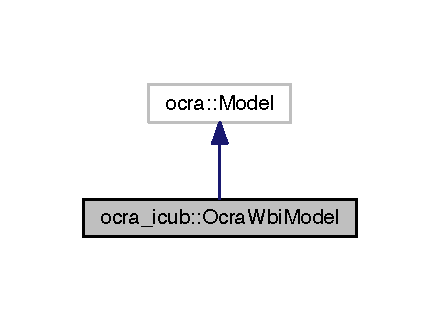
\includegraphics[width=211pt]{classocra__icub_1_1OcraWbiModel__inherit__graph}
\end{center}
\end{figure}


Collaboration diagram for ocra\+\_\+icub\+:\+:Ocra\+Wbi\+Model\+:\nopagebreak
\begin{figure}[H]
\begin{center}
\leavevmode
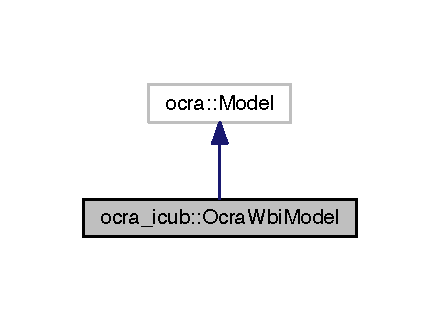
\includegraphics[width=211pt]{classocra__icub_1_1OcraWbiModel__coll__graph}
\end{center}
\end{figure}
\subsection*{Classes}
\begin{DoxyCompactItemize}
\item 
struct \hyperlink{structOcraWbiModel_1_1OcraWbiModel__pimpl}{Ocra\+Wbi\+Model\+\_\+pimpl}
\end{DoxyCompactItemize}
\subsection*{Public Member Functions}
\begin{DoxyCompactItemize}
\item 
\hyperlink{classocra__icub_1_1OcraWbiModel_a57a4f0f140f56d7ec0a00b31e16f9673}{Ocra\+Wbi\+Model} (const std\+::string \&robot\+Name, const int robot\+Num\+D\+OF, std\+::shared\+\_\+ptr$<$ wbi\+::whole\+Body\+Interface $>$ wbi, const bool free\+Root)
\item 
virtual \hyperlink{classocra__icub_1_1OcraWbiModel_ade110b2e003ccd49d2baa4f56a954e4b}{$\sim$\+Ocra\+Wbi\+Model} ()
\item 
virtual int \hyperlink{classocra__icub_1_1OcraWbiModel_a268f2b5b4dd0de558bfc9d8f9fa23db9}{nb\+Segments} () const
\item 
virtual const Eigen\+::\+Vector\+Xd \& \hyperlink{classocra__icub_1_1OcraWbiModel_acd7bfd155351337be585ae2171f9ddca}{get\+Actuated\+Dofs} () const
\item 
virtual const Eigen\+::\+Vector\+Xd \& \hyperlink{classocra__icub_1_1OcraWbiModel_a16eeeaeb928f3fa1f84273f8081453eb}{get\+Joint\+Lower\+Limits} () const
\item 
virtual const Eigen\+::\+Vector\+Xd \& \hyperlink{classocra__icub_1_1OcraWbiModel_a9752d5a831b935c61853b472fc4ff0ac}{get\+Joint\+Upper\+Limits} () const
\item 
virtual const Eigen\+::\+Vector\+Xd \& \hyperlink{classocra__icub_1_1OcraWbiModel_a87ccd2dd7f30319134cbf6431363b0ed}{get\+Joint\+Positions} () const
\item 
virtual const Eigen\+::\+Vector\+Xd \& \hyperlink{classocra__icub_1_1OcraWbiModel_a1dc6eb6a988b9833c33930e5e828e3c4}{get\+Joint\+Velocities} () const
\item 
virtual const Eigen\+::\+Vector\+Xd \& \hyperlink{classocra__icub_1_1OcraWbiModel_a25f75f03583958fddf4313007b0babdb}{get\+Joint\+Torques} () const
\item 
virtual const Eigen\+::\+Displacementd \& \hyperlink{classocra__icub_1_1OcraWbiModel_a1e48e56afb9ff2904785d5878d1021a9}{get\+Free\+Flyer\+Position} () const
\item 
virtual const Eigen\+::\+Twistd \& \hyperlink{classocra__icub_1_1OcraWbiModel_a6f87ccbf428eed32efb5424ec57eb3c3}{get\+Free\+Flyer\+Velocity} () const
\item 
virtual const std\+::string \& \hyperlink{classocra__icub_1_1OcraWbiModel_a9c5ca5123a2582bb43785db6d61413ea}{get\+Joint\+Name} (int index) const
\item 
virtual const int \hyperlink{classocra__icub_1_1OcraWbiModel_a9750492360a40e1b182ab05d19526ba2}{get\+Segment\+Index} (std\+::string segment\+Name) const
\item 
virtual const Eigen\+::\+Matrix\+Xd \& \hyperlink{classocra__icub_1_1OcraWbiModel_a019c1b4e52bad759d31d9ac60a268ab2}{get\+Inertia\+Matrix} () const
\item 
virtual const Eigen\+::\+Matrix\+Xd \& \hyperlink{classocra__icub_1_1OcraWbiModel_abba2c3248a9e526e98aa54935c75e84e}{get\+Inertia\+Matrix\+Inverse} () const
\item 
virtual const Eigen\+::\+Matrix\+Xd \& \hyperlink{classocra__icub_1_1OcraWbiModel_abe5946b7948e22fedfd09575fd4edbf7}{get\+Damping\+Matrix} () const
\item 
virtual const Eigen\+::\+Vector\+Xd \& \hyperlink{classocra__icub_1_1OcraWbiModel_a5802b0c6f4a8221e681fa41558f1b57c}{get\+Non\+Linear\+Terms} () const
\item 
virtual const Eigen\+::\+Vector\+Xd \& \hyperlink{classocra__icub_1_1OcraWbiModel_a08c2f48dfb8a6239efaa3d32cc92fa10}{get\+Linear\+Terms} () const
\item 
virtual const Eigen\+::\+Vector\+Xd \& \hyperlink{classocra__icub_1_1OcraWbiModel_a3457af2956db10e303a65886c62c076d}{get\+Gravity\+Terms} () const
\item 
virtual double \hyperlink{classocra__icub_1_1OcraWbiModel_a0d87a5d9c814db9ff24504890ef10395}{get\+Mass} () const
\item 
virtual const Eigen\+::\+Vector3d \& \hyperlink{classocra__icub_1_1OcraWbiModel_ac7f1d9d4677358db4c0c34ade2f645bd}{get\+Co\+M\+Position} () const
\item 
virtual const Eigen\+::\+Vector3d \& \hyperlink{classocra__icub_1_1OcraWbiModel_a08a0b1a4be74a6456162d60e38d470cd}{get\+Co\+M\+Velocity} () const
\item 
virtual const Eigen\+::\+Vector3d \& \hyperlink{classocra__icub_1_1OcraWbiModel_a38ee68461d9c5d6fccd876321fb0163a}{get\+Co\+M\+Jdot\+Qdot} () const
\item 
virtual const Eigen\+::\+Matrix$<$ double, 3, Eigen\+::\+Dynamic $>$ \& \hyperlink{classocra__icub_1_1OcraWbiModel_afc4580224117e18bcbed51a478da22f4}{get\+Co\+M\+Jacobian} () const
\item 
virtual const Eigen\+::\+Matrix$<$ double, 3, Eigen\+::\+Dynamic $>$ \& \hyperlink{classocra__icub_1_1OcraWbiModel_a216eae4ac21f869688b8eaf88e05b99b}{get\+Co\+M\+Jacobian\+Dot} () const
\item 
virtual const Eigen\+::\+Vector3d \& \hyperlink{classocra__icub_1_1OcraWbiModel_a48de3ef0a8531b4f1f68d4d53288b1e4}{get\+Co\+M\+Angular\+Velocity} () const
\item 
virtual const Eigen\+::\+Matrix$<$ double, 3, Eigen\+::\+Dynamic $>$ \& \hyperlink{classocra__icub_1_1OcraWbiModel_aca6a017f40a432142653bf3fa50f425d}{get\+Co\+M\+Angular\+Jacobian} () const
\item 
virtual const Eigen\+::\+Displacementd \& \hyperlink{classocra__icub_1_1OcraWbiModel_acb6a8faee8b9f32fdea179c2103be606}{get\+Segment\+Position} (int index) const
\item 
virtual const Eigen\+::\+Twistd \& \hyperlink{classocra__icub_1_1OcraWbiModel_a30e1597e69afd309c648ce7e1036f899}{get\+Segment\+Velocity} (int index) const
\item 
virtual double \hyperlink{classocra__icub_1_1OcraWbiModel_a54db828a81022e7855845bb0ce9d22aa}{get\+Segment\+Mass} (int index) const
\item 
virtual const Eigen\+::\+Vector3d \& \hyperlink{classocra__icub_1_1OcraWbiModel_a40e740aac3a79f6e607768b5bae9affb}{get\+Segment\+CoM} (int index) const
\item 
virtual const Eigen\+::\+Matrix$<$ double, 6, 6 $>$ \& \hyperlink{classocra__icub_1_1OcraWbiModel_ac8cdf27453a0a6856d35bec89da2db40}{get\+Segment\+Mass\+Matrix} (int index) const
\item 
virtual const Eigen\+::\+Vector3d \& \hyperlink{classocra__icub_1_1OcraWbiModel_a38d92d1a46b637d47b4588725e5dec8e}{get\+Segment\+Moments\+Of\+Inertia} (int index) const
\item 
virtual const Eigen\+::\+Rotation3d \& \hyperlink{classocra__icub_1_1OcraWbiModel_aaba3e74c964c1b7b2645aeae5bb5ade9}{get\+Segment\+Inertia\+Axes} (int index) const
\item 
virtual const Eigen\+::\+Matrix$<$ double, 6, Eigen\+::\+Dynamic $>$ \& \hyperlink{classocra__icub_1_1OcraWbiModel_a46613002aff4de4170c671bb5a6eab5c}{get\+Segment\+Jacobian} (int index) const
\item 
virtual const Eigen\+::\+Matrix$<$ double, 6, Eigen\+::\+Dynamic $>$ \& \hyperlink{classocra__icub_1_1OcraWbiModel_ac1e91eca8bd09fee58de68e3a6c1b670}{get\+Segment\+Jacobian} (int index, wbi\+::\+Frame H\+\_\+world\+\_\+root) const
\item 
virtual const Eigen\+::\+Matrix$<$ double, 6, Eigen\+::\+Dynamic $>$ \& \hyperlink{classocra__icub_1_1OcraWbiModel_aa195933567eef064020e889f4ee7ad94}{get\+Segment\+Jdot} (int index) const
\item 
virtual const Eigen\+::\+Matrix$<$ double, 6, Eigen\+::\+Dynamic $>$ \& \hyperlink{classocra__icub_1_1OcraWbiModel_a80a97ad74f71529119c6417935ecbde1}{get\+Joint\+Jacobian} (int index) const
\item 
virtual const Eigen\+::\+Twistd \& \hyperlink{classocra__icub_1_1OcraWbiModel_ac013379f185b03cbf092c6388e21ddcc}{get\+Segment\+Jdot\+Qdot} (int index) const
\item 
void \hyperlink{classocra__icub_1_1OcraWbiModel_a309b3554c4eefda46c05b766476f40fb}{print\+All\+Data} ()
\end{DoxyCompactItemize}
\subsection*{Protected Member Functions}
\begin{DoxyCompactItemize}
\item 
virtual void \hyperlink{classocra__icub_1_1OcraWbiModel_a8639b19a514624953e5e58dbde1c8227}{do\+Set\+State} (const Eigen\+::\+Vector\+Xd \&q, const Eigen\+::\+Vector\+Xd \&q\+\_\+dot)
\item 
virtual void \hyperlink{classocra__icub_1_1OcraWbiModel_a411c844cbde565ed54a224e39a2e65c1}{do\+Set\+State} (const Eigen\+::\+Displacementd \&H\+\_\+root, const Eigen\+::\+Vector\+Xd \&q, const Eigen\+::\+Twistd \&T\+\_\+root, const Eigen\+::\+Vector\+Xd \&q\+\_\+dot)
\item 
virtual void \hyperlink{classocra__icub_1_1OcraWbiModel_a64d40044dff11a6302992d52f1dbde0d}{do\+Set\+Joint\+Positions} (const Eigen\+::\+Vector\+Xd \&q)
\item 
virtual void \hyperlink{classocra__icub_1_1OcraWbiModel_a26a758c5ecb02601c066bdfffe5db194}{do\+Set\+Joint\+Velocities} (const Eigen\+::\+Vector\+Xd \&dq)
\item 
virtual void \hyperlink{classocra__icub_1_1OcraWbiModel_aa2bb481dc7fdb55c363ac1a404a807e5}{do\+Set\+Free\+Flyer\+Position} (const Eigen\+::\+Displacementd \&Hroot)
\item 
virtual void \hyperlink{classocra__icub_1_1OcraWbiModel_af740a36f6cc2899dcd6f3507b9703c7f}{do\+Set\+Free\+Flyer\+Velocity} (const Eigen\+::\+Twistd \&Troot)
\item 
virtual int \hyperlink{classocra__icub_1_1OcraWbiModel_a2587c2c67336e33077d50dd0f5a9e36a}{do\+Get\+Segment\+Index} (const std\+::string \&name) const
\item 
virtual const std\+::string \& \hyperlink{classocra__icub_1_1OcraWbiModel_adaa942dfad4d88adec255f3eac59e443}{do\+Get\+Segment\+Name} (int index) const
\item 
virtual int \hyperlink{classocra__icub_1_1OcraWbiModel_a327862ec0da18711147d0ec62002fbef}{do\+Get\+Dof\+Index} (const std\+::string \&name) const
\item 
virtual const std\+::string \& \hyperlink{classocra__icub_1_1OcraWbiModel_a63909e361f9361a6b20be8c0121b6d3c}{do\+Get\+Dof\+Name} (int index) const
\item 
virtual const std\+::string \hyperlink{classocra__icub_1_1OcraWbiModel_ac32c3de3dd4eb7864e4e81df96785cb2}{do\+Segment\+Name} (const std\+::string \&name) const
\item 
virtual const std\+::string \hyperlink{classocra__icub_1_1OcraWbiModel_af65d4fd7cae0ed86ea2bb588a9e024f9}{do\+Dof\+Name} (const std\+::string \&name) const
\end{DoxyCompactItemize}
\subsection*{Private Attributes}
\begin{DoxyCompactItemize}
\item 
std\+::shared\+\_\+ptr$<$ wbi\+::whole\+Body\+Interface $>$ \hyperlink{classocra__icub_1_1OcraWbiModel_ae377f000580656227fa9ef69f2f2e71d}{robot}
\item 
boost\+::shared\+\_\+ptr$<$ \hyperlink{structOcraWbiModel_1_1OcraWbiModel__pimpl}{Ocra\+Wbi\+Model\+\_\+pimpl} $>$ \hyperlink{classocra__icub_1_1OcraWbiModel_ab649cb769ca4edd345b3c09c43a69bde}{owm\+\_\+pimpl}
\item 
yarp\+::os\+::\+Log \hyperlink{classocra__icub_1_1OcraWbiModel_a047fe9f9a96794af218ea844f09cd402}{y\+Log}
\end{DoxyCompactItemize}


\subsection{Constructor \& Destructor Documentation}
\hypertarget{classocra__icub_1_1OcraWbiModel_a57a4f0f140f56d7ec0a00b31e16f9673}{}\label{classocra__icub_1_1OcraWbiModel_a57a4f0f140f56d7ec0a00b31e16f9673} 
\index{ocra\+\_\+icub\+::\+Ocra\+Wbi\+Model@{ocra\+\_\+icub\+::\+Ocra\+Wbi\+Model}!Ocra\+Wbi\+Model@{Ocra\+Wbi\+Model}}
\index{Ocra\+Wbi\+Model@{Ocra\+Wbi\+Model}!ocra\+\_\+icub\+::\+Ocra\+Wbi\+Model@{ocra\+\_\+icub\+::\+Ocra\+Wbi\+Model}}
\subsubsection{\texorpdfstring{Ocra\+Wbi\+Model()}{OcraWbiModel()}}
{\footnotesize\ttfamily Ocra\+Wbi\+Model\+::\+Ocra\+Wbi\+Model (\begin{DoxyParamCaption}\item[{const std\+::string \&}]{robot\+Name,  }\item[{const int}]{robot\+Num\+D\+OF,  }\item[{std\+::shared\+\_\+ptr$<$ wbi\+::whole\+Body\+Interface $>$}]{wbi,  }\item[{const bool}]{free\+Root }\end{DoxyParamCaption})}

\hypertarget{classocra__icub_1_1OcraWbiModel_ade110b2e003ccd49d2baa4f56a954e4b}{}\label{classocra__icub_1_1OcraWbiModel_ade110b2e003ccd49d2baa4f56a954e4b} 
\index{ocra\+\_\+icub\+::\+Ocra\+Wbi\+Model@{ocra\+\_\+icub\+::\+Ocra\+Wbi\+Model}!````~Ocra\+Wbi\+Model@{$\sim$\+Ocra\+Wbi\+Model}}
\index{````~Ocra\+Wbi\+Model@{$\sim$\+Ocra\+Wbi\+Model}!ocra\+\_\+icub\+::\+Ocra\+Wbi\+Model@{ocra\+\_\+icub\+::\+Ocra\+Wbi\+Model}}
\subsubsection{\texorpdfstring{$\sim$\+Ocra\+Wbi\+Model()}{~OcraWbiModel()}}
{\footnotesize\ttfamily Ocra\+Wbi\+Model\+::$\sim$\+Ocra\+Wbi\+Model (\begin{DoxyParamCaption}{ }\end{DoxyParamCaption})\hspace{0.3cm}{\ttfamily [virtual]}}



\subsection{Member Function Documentation}
\hypertarget{classocra__icub_1_1OcraWbiModel_af65d4fd7cae0ed86ea2bb588a9e024f9}{}\label{classocra__icub_1_1OcraWbiModel_af65d4fd7cae0ed86ea2bb588a9e024f9} 
\index{ocra\+\_\+icub\+::\+Ocra\+Wbi\+Model@{ocra\+\_\+icub\+::\+Ocra\+Wbi\+Model}!do\+Dof\+Name@{do\+Dof\+Name}}
\index{do\+Dof\+Name@{do\+Dof\+Name}!ocra\+\_\+icub\+::\+Ocra\+Wbi\+Model@{ocra\+\_\+icub\+::\+Ocra\+Wbi\+Model}}
\subsubsection{\texorpdfstring{do\+Dof\+Name()}{doDofName()}}
{\footnotesize\ttfamily const std\+::string Ocra\+Wbi\+Model\+::do\+Dof\+Name (\begin{DoxyParamCaption}\item[{const std\+::string \&}]{name }\end{DoxyParamCaption}) const\hspace{0.3cm}{\ttfamily [protected]}, {\ttfamily [virtual]}}

\hypertarget{classocra__icub_1_1OcraWbiModel_a327862ec0da18711147d0ec62002fbef}{}\label{classocra__icub_1_1OcraWbiModel_a327862ec0da18711147d0ec62002fbef} 
\index{ocra\+\_\+icub\+::\+Ocra\+Wbi\+Model@{ocra\+\_\+icub\+::\+Ocra\+Wbi\+Model}!do\+Get\+Dof\+Index@{do\+Get\+Dof\+Index}}
\index{do\+Get\+Dof\+Index@{do\+Get\+Dof\+Index}!ocra\+\_\+icub\+::\+Ocra\+Wbi\+Model@{ocra\+\_\+icub\+::\+Ocra\+Wbi\+Model}}
\subsubsection{\texorpdfstring{do\+Get\+Dof\+Index()}{doGetDofIndex()}}
{\footnotesize\ttfamily int Ocra\+Wbi\+Model\+::do\+Get\+Dof\+Index (\begin{DoxyParamCaption}\item[{const std\+::string \&}]{name }\end{DoxyParamCaption}) const\hspace{0.3cm}{\ttfamily [protected]}, {\ttfamily [virtual]}}

\hypertarget{classocra__icub_1_1OcraWbiModel_a63909e361f9361a6b20be8c0121b6d3c}{}\label{classocra__icub_1_1OcraWbiModel_a63909e361f9361a6b20be8c0121b6d3c} 
\index{ocra\+\_\+icub\+::\+Ocra\+Wbi\+Model@{ocra\+\_\+icub\+::\+Ocra\+Wbi\+Model}!do\+Get\+Dof\+Name@{do\+Get\+Dof\+Name}}
\index{do\+Get\+Dof\+Name@{do\+Get\+Dof\+Name}!ocra\+\_\+icub\+::\+Ocra\+Wbi\+Model@{ocra\+\_\+icub\+::\+Ocra\+Wbi\+Model}}
\subsubsection{\texorpdfstring{do\+Get\+Dof\+Name()}{doGetDofName()}}
{\footnotesize\ttfamily const std\+::string \& Ocra\+Wbi\+Model\+::do\+Get\+Dof\+Name (\begin{DoxyParamCaption}\item[{int}]{index }\end{DoxyParamCaption}) const\hspace{0.3cm}{\ttfamily [protected]}, {\ttfamily [virtual]}}

\hypertarget{classocra__icub_1_1OcraWbiModel_a2587c2c67336e33077d50dd0f5a9e36a}{}\label{classocra__icub_1_1OcraWbiModel_a2587c2c67336e33077d50dd0f5a9e36a} 
\index{ocra\+\_\+icub\+::\+Ocra\+Wbi\+Model@{ocra\+\_\+icub\+::\+Ocra\+Wbi\+Model}!do\+Get\+Segment\+Index@{do\+Get\+Segment\+Index}}
\index{do\+Get\+Segment\+Index@{do\+Get\+Segment\+Index}!ocra\+\_\+icub\+::\+Ocra\+Wbi\+Model@{ocra\+\_\+icub\+::\+Ocra\+Wbi\+Model}}
\subsubsection{\texorpdfstring{do\+Get\+Segment\+Index()}{doGetSegmentIndex()}}
{\footnotesize\ttfamily int Ocra\+Wbi\+Model\+::do\+Get\+Segment\+Index (\begin{DoxyParamCaption}\item[{const std\+::string \&}]{name }\end{DoxyParamCaption}) const\hspace{0.3cm}{\ttfamily [protected]}, {\ttfamily [virtual]}}

\hypertarget{classocra__icub_1_1OcraWbiModel_adaa942dfad4d88adec255f3eac59e443}{}\label{classocra__icub_1_1OcraWbiModel_adaa942dfad4d88adec255f3eac59e443} 
\index{ocra\+\_\+icub\+::\+Ocra\+Wbi\+Model@{ocra\+\_\+icub\+::\+Ocra\+Wbi\+Model}!do\+Get\+Segment\+Name@{do\+Get\+Segment\+Name}}
\index{do\+Get\+Segment\+Name@{do\+Get\+Segment\+Name}!ocra\+\_\+icub\+::\+Ocra\+Wbi\+Model@{ocra\+\_\+icub\+::\+Ocra\+Wbi\+Model}}
\subsubsection{\texorpdfstring{do\+Get\+Segment\+Name()}{doGetSegmentName()}}
{\footnotesize\ttfamily const std\+::string \& Ocra\+Wbi\+Model\+::do\+Get\+Segment\+Name (\begin{DoxyParamCaption}\item[{int}]{index }\end{DoxyParamCaption}) const\hspace{0.3cm}{\ttfamily [protected]}, {\ttfamily [virtual]}}

\hypertarget{classocra__icub_1_1OcraWbiModel_ac32c3de3dd4eb7864e4e81df96785cb2}{}\label{classocra__icub_1_1OcraWbiModel_ac32c3de3dd4eb7864e4e81df96785cb2} 
\index{ocra\+\_\+icub\+::\+Ocra\+Wbi\+Model@{ocra\+\_\+icub\+::\+Ocra\+Wbi\+Model}!do\+Segment\+Name@{do\+Segment\+Name}}
\index{do\+Segment\+Name@{do\+Segment\+Name}!ocra\+\_\+icub\+::\+Ocra\+Wbi\+Model@{ocra\+\_\+icub\+::\+Ocra\+Wbi\+Model}}
\subsubsection{\texorpdfstring{do\+Segment\+Name()}{doSegmentName()}}
{\footnotesize\ttfamily const std\+::string Ocra\+Wbi\+Model\+::do\+Segment\+Name (\begin{DoxyParamCaption}\item[{const std\+::string \&}]{name }\end{DoxyParamCaption}) const\hspace{0.3cm}{\ttfamily [protected]}, {\ttfamily [virtual]}}

\hypertarget{classocra__icub_1_1OcraWbiModel_aa2bb481dc7fdb55c363ac1a404a807e5}{}\label{classocra__icub_1_1OcraWbiModel_aa2bb481dc7fdb55c363ac1a404a807e5} 
\index{ocra\+\_\+icub\+::\+Ocra\+Wbi\+Model@{ocra\+\_\+icub\+::\+Ocra\+Wbi\+Model}!do\+Set\+Free\+Flyer\+Position@{do\+Set\+Free\+Flyer\+Position}}
\index{do\+Set\+Free\+Flyer\+Position@{do\+Set\+Free\+Flyer\+Position}!ocra\+\_\+icub\+::\+Ocra\+Wbi\+Model@{ocra\+\_\+icub\+::\+Ocra\+Wbi\+Model}}
\subsubsection{\texorpdfstring{do\+Set\+Free\+Flyer\+Position()}{doSetFreeFlyerPosition()}}
{\footnotesize\ttfamily void Ocra\+Wbi\+Model\+::do\+Set\+Free\+Flyer\+Position (\begin{DoxyParamCaption}\item[{const Eigen\+::\+Displacementd \&}]{Hroot }\end{DoxyParamCaption})\hspace{0.3cm}{\ttfamily [protected]}, {\ttfamily [virtual]}}

\hypertarget{classocra__icub_1_1OcraWbiModel_af740a36f6cc2899dcd6f3507b9703c7f}{}\label{classocra__icub_1_1OcraWbiModel_af740a36f6cc2899dcd6f3507b9703c7f} 
\index{ocra\+\_\+icub\+::\+Ocra\+Wbi\+Model@{ocra\+\_\+icub\+::\+Ocra\+Wbi\+Model}!do\+Set\+Free\+Flyer\+Velocity@{do\+Set\+Free\+Flyer\+Velocity}}
\index{do\+Set\+Free\+Flyer\+Velocity@{do\+Set\+Free\+Flyer\+Velocity}!ocra\+\_\+icub\+::\+Ocra\+Wbi\+Model@{ocra\+\_\+icub\+::\+Ocra\+Wbi\+Model}}
\subsubsection{\texorpdfstring{do\+Set\+Free\+Flyer\+Velocity()}{doSetFreeFlyerVelocity()}}
{\footnotesize\ttfamily void Ocra\+Wbi\+Model\+::do\+Set\+Free\+Flyer\+Velocity (\begin{DoxyParamCaption}\item[{const Eigen\+::\+Twistd \&}]{Troot }\end{DoxyParamCaption})\hspace{0.3cm}{\ttfamily [protected]}, {\ttfamily [virtual]}}

\hypertarget{classocra__icub_1_1OcraWbiModel_a64d40044dff11a6302992d52f1dbde0d}{}\label{classocra__icub_1_1OcraWbiModel_a64d40044dff11a6302992d52f1dbde0d} 
\index{ocra\+\_\+icub\+::\+Ocra\+Wbi\+Model@{ocra\+\_\+icub\+::\+Ocra\+Wbi\+Model}!do\+Set\+Joint\+Positions@{do\+Set\+Joint\+Positions}}
\index{do\+Set\+Joint\+Positions@{do\+Set\+Joint\+Positions}!ocra\+\_\+icub\+::\+Ocra\+Wbi\+Model@{ocra\+\_\+icub\+::\+Ocra\+Wbi\+Model}}
\subsubsection{\texorpdfstring{do\+Set\+Joint\+Positions()}{doSetJointPositions()}}
{\footnotesize\ttfamily void Ocra\+Wbi\+Model\+::do\+Set\+Joint\+Positions (\begin{DoxyParamCaption}\item[{const Eigen\+::\+Vector\+Xd \&}]{q }\end{DoxyParamCaption})\hspace{0.3cm}{\ttfamily [protected]}, {\ttfamily [virtual]}}

\hypertarget{classocra__icub_1_1OcraWbiModel_a26a758c5ecb02601c066bdfffe5db194}{}\label{classocra__icub_1_1OcraWbiModel_a26a758c5ecb02601c066bdfffe5db194} 
\index{ocra\+\_\+icub\+::\+Ocra\+Wbi\+Model@{ocra\+\_\+icub\+::\+Ocra\+Wbi\+Model}!do\+Set\+Joint\+Velocities@{do\+Set\+Joint\+Velocities}}
\index{do\+Set\+Joint\+Velocities@{do\+Set\+Joint\+Velocities}!ocra\+\_\+icub\+::\+Ocra\+Wbi\+Model@{ocra\+\_\+icub\+::\+Ocra\+Wbi\+Model}}
\subsubsection{\texorpdfstring{do\+Set\+Joint\+Velocities()}{doSetJointVelocities()}}
{\footnotesize\ttfamily void Ocra\+Wbi\+Model\+::do\+Set\+Joint\+Velocities (\begin{DoxyParamCaption}\item[{const Eigen\+::\+Vector\+Xd \&}]{dq }\end{DoxyParamCaption})\hspace{0.3cm}{\ttfamily [protected]}, {\ttfamily [virtual]}}

\hypertarget{classocra__icub_1_1OcraWbiModel_a8639b19a514624953e5e58dbde1c8227}{}\label{classocra__icub_1_1OcraWbiModel_a8639b19a514624953e5e58dbde1c8227} 
\index{ocra\+\_\+icub\+::\+Ocra\+Wbi\+Model@{ocra\+\_\+icub\+::\+Ocra\+Wbi\+Model}!do\+Set\+State@{do\+Set\+State}}
\index{do\+Set\+State@{do\+Set\+State}!ocra\+\_\+icub\+::\+Ocra\+Wbi\+Model@{ocra\+\_\+icub\+::\+Ocra\+Wbi\+Model}}
\subsubsection{\texorpdfstring{do\+Set\+State()}{doSetState()}\hspace{0.1cm}{\footnotesize\ttfamily [1/2]}}
{\footnotesize\ttfamily void Ocra\+Wbi\+Model\+::do\+Set\+State (\begin{DoxyParamCaption}\item[{const Eigen\+::\+Vector\+Xd \&}]{q,  }\item[{const Eigen\+::\+Vector\+Xd \&}]{q\+\_\+dot }\end{DoxyParamCaption})\hspace{0.3cm}{\ttfamily [protected]}, {\ttfamily [virtual]}}

\hypertarget{classocra__icub_1_1OcraWbiModel_a411c844cbde565ed54a224e39a2e65c1}{}\label{classocra__icub_1_1OcraWbiModel_a411c844cbde565ed54a224e39a2e65c1} 
\index{ocra\+\_\+icub\+::\+Ocra\+Wbi\+Model@{ocra\+\_\+icub\+::\+Ocra\+Wbi\+Model}!do\+Set\+State@{do\+Set\+State}}
\index{do\+Set\+State@{do\+Set\+State}!ocra\+\_\+icub\+::\+Ocra\+Wbi\+Model@{ocra\+\_\+icub\+::\+Ocra\+Wbi\+Model}}
\subsubsection{\texorpdfstring{do\+Set\+State()}{doSetState()}\hspace{0.1cm}{\footnotesize\ttfamily [2/2]}}
{\footnotesize\ttfamily void Ocra\+Wbi\+Model\+::do\+Set\+State (\begin{DoxyParamCaption}\item[{const Eigen\+::\+Displacementd \&}]{H\+\_\+root,  }\item[{const Eigen\+::\+Vector\+Xd \&}]{q,  }\item[{const Eigen\+::\+Twistd \&}]{T\+\_\+root,  }\item[{const Eigen\+::\+Vector\+Xd \&}]{q\+\_\+dot }\end{DoxyParamCaption})\hspace{0.3cm}{\ttfamily [protected]}, {\ttfamily [virtual]}}

\hypertarget{classocra__icub_1_1OcraWbiModel_acd7bfd155351337be585ae2171f9ddca}{}\label{classocra__icub_1_1OcraWbiModel_acd7bfd155351337be585ae2171f9ddca} 
\index{ocra\+\_\+icub\+::\+Ocra\+Wbi\+Model@{ocra\+\_\+icub\+::\+Ocra\+Wbi\+Model}!get\+Actuated\+Dofs@{get\+Actuated\+Dofs}}
\index{get\+Actuated\+Dofs@{get\+Actuated\+Dofs}!ocra\+\_\+icub\+::\+Ocra\+Wbi\+Model@{ocra\+\_\+icub\+::\+Ocra\+Wbi\+Model}}
\subsubsection{\texorpdfstring{get\+Actuated\+Dofs()}{getActuatedDofs()}}
{\footnotesize\ttfamily const Eigen\+::\+Vector\+Xd \& Ocra\+Wbi\+Model\+::get\+Actuated\+Dofs (\begin{DoxyParamCaption}{ }\end{DoxyParamCaption}) const\hspace{0.3cm}{\ttfamily [virtual]}}

\hypertarget{classocra__icub_1_1OcraWbiModel_aca6a017f40a432142653bf3fa50f425d}{}\label{classocra__icub_1_1OcraWbiModel_aca6a017f40a432142653bf3fa50f425d} 
\index{ocra\+\_\+icub\+::\+Ocra\+Wbi\+Model@{ocra\+\_\+icub\+::\+Ocra\+Wbi\+Model}!get\+Co\+M\+Angular\+Jacobian@{get\+Co\+M\+Angular\+Jacobian}}
\index{get\+Co\+M\+Angular\+Jacobian@{get\+Co\+M\+Angular\+Jacobian}!ocra\+\_\+icub\+::\+Ocra\+Wbi\+Model@{ocra\+\_\+icub\+::\+Ocra\+Wbi\+Model}}
\subsubsection{\texorpdfstring{get\+Co\+M\+Angular\+Jacobian()}{getCoMAngularJacobian()}}
{\footnotesize\ttfamily const Eigen\+::\+Matrix$<$ double, \hyperlink{OcraWbiModel_8cpp_a72cb22de2538ae949cc73fa3d7c33bdc}{C\+O\+M\+\_\+\+P\+O\+S\+\_\+\+D\+IM}, Eigen\+::\+Dynamic $>$ \& Ocra\+Wbi\+Model\+::get\+Co\+M\+Angular\+Jacobian (\begin{DoxyParamCaption}{ }\end{DoxyParamCaption}) const\hspace{0.3cm}{\ttfamily [virtual]}}

\hypertarget{classocra__icub_1_1OcraWbiModel_a48de3ef0a8531b4f1f68d4d53288b1e4}{}\label{classocra__icub_1_1OcraWbiModel_a48de3ef0a8531b4f1f68d4d53288b1e4} 
\index{ocra\+\_\+icub\+::\+Ocra\+Wbi\+Model@{ocra\+\_\+icub\+::\+Ocra\+Wbi\+Model}!get\+Co\+M\+Angular\+Velocity@{get\+Co\+M\+Angular\+Velocity}}
\index{get\+Co\+M\+Angular\+Velocity@{get\+Co\+M\+Angular\+Velocity}!ocra\+\_\+icub\+::\+Ocra\+Wbi\+Model@{ocra\+\_\+icub\+::\+Ocra\+Wbi\+Model}}
\subsubsection{\texorpdfstring{get\+Co\+M\+Angular\+Velocity()}{getCoMAngularVelocity()}}
{\footnotesize\ttfamily const Eigen\+::\+Vector3d \& Ocra\+Wbi\+Model\+::get\+Co\+M\+Angular\+Velocity (\begin{DoxyParamCaption}{ }\end{DoxyParamCaption}) const\hspace{0.3cm}{\ttfamily [virtual]}}

\hypertarget{classocra__icub_1_1OcraWbiModel_afc4580224117e18bcbed51a478da22f4}{}\label{classocra__icub_1_1OcraWbiModel_afc4580224117e18bcbed51a478da22f4} 
\index{ocra\+\_\+icub\+::\+Ocra\+Wbi\+Model@{ocra\+\_\+icub\+::\+Ocra\+Wbi\+Model}!get\+Co\+M\+Jacobian@{get\+Co\+M\+Jacobian}}
\index{get\+Co\+M\+Jacobian@{get\+Co\+M\+Jacobian}!ocra\+\_\+icub\+::\+Ocra\+Wbi\+Model@{ocra\+\_\+icub\+::\+Ocra\+Wbi\+Model}}
\subsubsection{\texorpdfstring{get\+Co\+M\+Jacobian()}{getCoMJacobian()}}
{\footnotesize\ttfamily const Eigen\+::\+Matrix$<$ double, \hyperlink{OcraWbiModel_8cpp_a72cb22de2538ae949cc73fa3d7c33bdc}{C\+O\+M\+\_\+\+P\+O\+S\+\_\+\+D\+IM}, Eigen\+::\+Dynamic $>$ \& Ocra\+Wbi\+Model\+::get\+Co\+M\+Jacobian (\begin{DoxyParamCaption}{ }\end{DoxyParamCaption}) const\hspace{0.3cm}{\ttfamily [virtual]}}

\hypertarget{classocra__icub_1_1OcraWbiModel_a216eae4ac21f869688b8eaf88e05b99b}{}\label{classocra__icub_1_1OcraWbiModel_a216eae4ac21f869688b8eaf88e05b99b} 
\index{ocra\+\_\+icub\+::\+Ocra\+Wbi\+Model@{ocra\+\_\+icub\+::\+Ocra\+Wbi\+Model}!get\+Co\+M\+Jacobian\+Dot@{get\+Co\+M\+Jacobian\+Dot}}
\index{get\+Co\+M\+Jacobian\+Dot@{get\+Co\+M\+Jacobian\+Dot}!ocra\+\_\+icub\+::\+Ocra\+Wbi\+Model@{ocra\+\_\+icub\+::\+Ocra\+Wbi\+Model}}
\subsubsection{\texorpdfstring{get\+Co\+M\+Jacobian\+Dot()}{getCoMJacobianDot()}}
{\footnotesize\ttfamily const Eigen\+::\+Matrix$<$ double, \hyperlink{OcraWbiModel_8cpp_a72cb22de2538ae949cc73fa3d7c33bdc}{C\+O\+M\+\_\+\+P\+O\+S\+\_\+\+D\+IM}, Eigen\+::\+Dynamic $>$ \& Ocra\+Wbi\+Model\+::get\+Co\+M\+Jacobian\+Dot (\begin{DoxyParamCaption}{ }\end{DoxyParamCaption}) const\hspace{0.3cm}{\ttfamily [virtual]}}

\hypertarget{classocra__icub_1_1OcraWbiModel_a38ee68461d9c5d6fccd876321fb0163a}{}\label{classocra__icub_1_1OcraWbiModel_a38ee68461d9c5d6fccd876321fb0163a} 
\index{ocra\+\_\+icub\+::\+Ocra\+Wbi\+Model@{ocra\+\_\+icub\+::\+Ocra\+Wbi\+Model}!get\+Co\+M\+Jdot\+Qdot@{get\+Co\+M\+Jdot\+Qdot}}
\index{get\+Co\+M\+Jdot\+Qdot@{get\+Co\+M\+Jdot\+Qdot}!ocra\+\_\+icub\+::\+Ocra\+Wbi\+Model@{ocra\+\_\+icub\+::\+Ocra\+Wbi\+Model}}
\subsubsection{\texorpdfstring{get\+Co\+M\+Jdot\+Qdot()}{getCoMJdotQdot()}}
{\footnotesize\ttfamily const Eigen\+::\+Vector3d \& Ocra\+Wbi\+Model\+::get\+Co\+M\+Jdot\+Qdot (\begin{DoxyParamCaption}{ }\end{DoxyParamCaption}) const\hspace{0.3cm}{\ttfamily [virtual]}}

\hypertarget{classocra__icub_1_1OcraWbiModel_ac7f1d9d4677358db4c0c34ade2f645bd}{}\label{classocra__icub_1_1OcraWbiModel_ac7f1d9d4677358db4c0c34ade2f645bd} 
\index{ocra\+\_\+icub\+::\+Ocra\+Wbi\+Model@{ocra\+\_\+icub\+::\+Ocra\+Wbi\+Model}!get\+Co\+M\+Position@{get\+Co\+M\+Position}}
\index{get\+Co\+M\+Position@{get\+Co\+M\+Position}!ocra\+\_\+icub\+::\+Ocra\+Wbi\+Model@{ocra\+\_\+icub\+::\+Ocra\+Wbi\+Model}}
\subsubsection{\texorpdfstring{get\+Co\+M\+Position()}{getCoMPosition()}}
{\footnotesize\ttfamily const Eigen\+::\+Vector3d \& Ocra\+Wbi\+Model\+::get\+Co\+M\+Position (\begin{DoxyParamCaption}{ }\end{DoxyParamCaption}) const\hspace{0.3cm}{\ttfamily [virtual]}}

\hypertarget{classocra__icub_1_1OcraWbiModel_a08a0b1a4be74a6456162d60e38d470cd}{}\label{classocra__icub_1_1OcraWbiModel_a08a0b1a4be74a6456162d60e38d470cd} 
\index{ocra\+\_\+icub\+::\+Ocra\+Wbi\+Model@{ocra\+\_\+icub\+::\+Ocra\+Wbi\+Model}!get\+Co\+M\+Velocity@{get\+Co\+M\+Velocity}}
\index{get\+Co\+M\+Velocity@{get\+Co\+M\+Velocity}!ocra\+\_\+icub\+::\+Ocra\+Wbi\+Model@{ocra\+\_\+icub\+::\+Ocra\+Wbi\+Model}}
\subsubsection{\texorpdfstring{get\+Co\+M\+Velocity()}{getCoMVelocity()}}
{\footnotesize\ttfamily const Eigen\+::\+Vector3d \& Ocra\+Wbi\+Model\+::get\+Co\+M\+Velocity (\begin{DoxyParamCaption}{ }\end{DoxyParamCaption}) const\hspace{0.3cm}{\ttfamily [virtual]}}

\hypertarget{classocra__icub_1_1OcraWbiModel_abe5946b7948e22fedfd09575fd4edbf7}{}\label{classocra__icub_1_1OcraWbiModel_abe5946b7948e22fedfd09575fd4edbf7} 
\index{ocra\+\_\+icub\+::\+Ocra\+Wbi\+Model@{ocra\+\_\+icub\+::\+Ocra\+Wbi\+Model}!get\+Damping\+Matrix@{get\+Damping\+Matrix}}
\index{get\+Damping\+Matrix@{get\+Damping\+Matrix}!ocra\+\_\+icub\+::\+Ocra\+Wbi\+Model@{ocra\+\_\+icub\+::\+Ocra\+Wbi\+Model}}
\subsubsection{\texorpdfstring{get\+Damping\+Matrix()}{getDampingMatrix()}}
{\footnotesize\ttfamily const Eigen\+::\+Matrix\+Xd \& Ocra\+Wbi\+Model\+::get\+Damping\+Matrix (\begin{DoxyParamCaption}{ }\end{DoxyParamCaption}) const\hspace{0.3cm}{\ttfamily [virtual]}}

\hypertarget{classocra__icub_1_1OcraWbiModel_a1e48e56afb9ff2904785d5878d1021a9}{}\label{classocra__icub_1_1OcraWbiModel_a1e48e56afb9ff2904785d5878d1021a9} 
\index{ocra\+\_\+icub\+::\+Ocra\+Wbi\+Model@{ocra\+\_\+icub\+::\+Ocra\+Wbi\+Model}!get\+Free\+Flyer\+Position@{get\+Free\+Flyer\+Position}}
\index{get\+Free\+Flyer\+Position@{get\+Free\+Flyer\+Position}!ocra\+\_\+icub\+::\+Ocra\+Wbi\+Model@{ocra\+\_\+icub\+::\+Ocra\+Wbi\+Model}}
\subsubsection{\texorpdfstring{get\+Free\+Flyer\+Position()}{getFreeFlyerPosition()}}
{\footnotesize\ttfamily const Eigen\+::\+Displacementd \& Ocra\+Wbi\+Model\+::get\+Free\+Flyer\+Position (\begin{DoxyParamCaption}{ }\end{DoxyParamCaption}) const\hspace{0.3cm}{\ttfamily [virtual]}}

\hypertarget{classocra__icub_1_1OcraWbiModel_a6f87ccbf428eed32efb5424ec57eb3c3}{}\label{classocra__icub_1_1OcraWbiModel_a6f87ccbf428eed32efb5424ec57eb3c3} 
\index{ocra\+\_\+icub\+::\+Ocra\+Wbi\+Model@{ocra\+\_\+icub\+::\+Ocra\+Wbi\+Model}!get\+Free\+Flyer\+Velocity@{get\+Free\+Flyer\+Velocity}}
\index{get\+Free\+Flyer\+Velocity@{get\+Free\+Flyer\+Velocity}!ocra\+\_\+icub\+::\+Ocra\+Wbi\+Model@{ocra\+\_\+icub\+::\+Ocra\+Wbi\+Model}}
\subsubsection{\texorpdfstring{get\+Free\+Flyer\+Velocity()}{getFreeFlyerVelocity()}}
{\footnotesize\ttfamily const Eigen\+::\+Twistd \& Ocra\+Wbi\+Model\+::get\+Free\+Flyer\+Velocity (\begin{DoxyParamCaption}{ }\end{DoxyParamCaption}) const\hspace{0.3cm}{\ttfamily [virtual]}}

\hypertarget{classocra__icub_1_1OcraWbiModel_a3457af2956db10e303a65886c62c076d}{}\label{classocra__icub_1_1OcraWbiModel_a3457af2956db10e303a65886c62c076d} 
\index{ocra\+\_\+icub\+::\+Ocra\+Wbi\+Model@{ocra\+\_\+icub\+::\+Ocra\+Wbi\+Model}!get\+Gravity\+Terms@{get\+Gravity\+Terms}}
\index{get\+Gravity\+Terms@{get\+Gravity\+Terms}!ocra\+\_\+icub\+::\+Ocra\+Wbi\+Model@{ocra\+\_\+icub\+::\+Ocra\+Wbi\+Model}}
\subsubsection{\texorpdfstring{get\+Gravity\+Terms()}{getGravityTerms()}}
{\footnotesize\ttfamily const Eigen\+::\+Vector\+Xd \& Ocra\+Wbi\+Model\+::get\+Gravity\+Terms (\begin{DoxyParamCaption}{ }\end{DoxyParamCaption}) const\hspace{0.3cm}{\ttfamily [virtual]}}

\hypertarget{classocra__icub_1_1OcraWbiModel_a019c1b4e52bad759d31d9ac60a268ab2}{}\label{classocra__icub_1_1OcraWbiModel_a019c1b4e52bad759d31d9ac60a268ab2} 
\index{ocra\+\_\+icub\+::\+Ocra\+Wbi\+Model@{ocra\+\_\+icub\+::\+Ocra\+Wbi\+Model}!get\+Inertia\+Matrix@{get\+Inertia\+Matrix}}
\index{get\+Inertia\+Matrix@{get\+Inertia\+Matrix}!ocra\+\_\+icub\+::\+Ocra\+Wbi\+Model@{ocra\+\_\+icub\+::\+Ocra\+Wbi\+Model}}
\subsubsection{\texorpdfstring{get\+Inertia\+Matrix()}{getInertiaMatrix()}}
{\footnotesize\ttfamily const Eigen\+::\+Matrix\+Xd \& Ocra\+Wbi\+Model\+::get\+Inertia\+Matrix (\begin{DoxyParamCaption}{ }\end{DoxyParamCaption}) const\hspace{0.3cm}{\ttfamily [virtual]}}

\hypertarget{classocra__icub_1_1OcraWbiModel_abba2c3248a9e526e98aa54935c75e84e}{}\label{classocra__icub_1_1OcraWbiModel_abba2c3248a9e526e98aa54935c75e84e} 
\index{ocra\+\_\+icub\+::\+Ocra\+Wbi\+Model@{ocra\+\_\+icub\+::\+Ocra\+Wbi\+Model}!get\+Inertia\+Matrix\+Inverse@{get\+Inertia\+Matrix\+Inverse}}
\index{get\+Inertia\+Matrix\+Inverse@{get\+Inertia\+Matrix\+Inverse}!ocra\+\_\+icub\+::\+Ocra\+Wbi\+Model@{ocra\+\_\+icub\+::\+Ocra\+Wbi\+Model}}
\subsubsection{\texorpdfstring{get\+Inertia\+Matrix\+Inverse()}{getInertiaMatrixInverse()}}
{\footnotesize\ttfamily const Eigen\+::\+Matrix\+Xd \& Ocra\+Wbi\+Model\+::get\+Inertia\+Matrix\+Inverse (\begin{DoxyParamCaption}{ }\end{DoxyParamCaption}) const\hspace{0.3cm}{\ttfamily [virtual]}}

\hypertarget{classocra__icub_1_1OcraWbiModel_a80a97ad74f71529119c6417935ecbde1}{}\label{classocra__icub_1_1OcraWbiModel_a80a97ad74f71529119c6417935ecbde1} 
\index{ocra\+\_\+icub\+::\+Ocra\+Wbi\+Model@{ocra\+\_\+icub\+::\+Ocra\+Wbi\+Model}!get\+Joint\+Jacobian@{get\+Joint\+Jacobian}}
\index{get\+Joint\+Jacobian@{get\+Joint\+Jacobian}!ocra\+\_\+icub\+::\+Ocra\+Wbi\+Model@{ocra\+\_\+icub\+::\+Ocra\+Wbi\+Model}}
\subsubsection{\texorpdfstring{get\+Joint\+Jacobian()}{getJointJacobian()}}
{\footnotesize\ttfamily const Eigen\+::\+Matrix$<$ double, 6, Eigen\+::\+Dynamic $>$ \& Ocra\+Wbi\+Model\+::get\+Joint\+Jacobian (\begin{DoxyParamCaption}\item[{int}]{index }\end{DoxyParamCaption}) const\hspace{0.3cm}{\ttfamily [virtual]}}

\hypertarget{classocra__icub_1_1OcraWbiModel_a16eeeaeb928f3fa1f84273f8081453eb}{}\label{classocra__icub_1_1OcraWbiModel_a16eeeaeb928f3fa1f84273f8081453eb} 
\index{ocra\+\_\+icub\+::\+Ocra\+Wbi\+Model@{ocra\+\_\+icub\+::\+Ocra\+Wbi\+Model}!get\+Joint\+Lower\+Limits@{get\+Joint\+Lower\+Limits}}
\index{get\+Joint\+Lower\+Limits@{get\+Joint\+Lower\+Limits}!ocra\+\_\+icub\+::\+Ocra\+Wbi\+Model@{ocra\+\_\+icub\+::\+Ocra\+Wbi\+Model}}
\subsubsection{\texorpdfstring{get\+Joint\+Lower\+Limits()}{getJointLowerLimits()}}
{\footnotesize\ttfamily const Eigen\+::\+Vector\+Xd \& Ocra\+Wbi\+Model\+::get\+Joint\+Lower\+Limits (\begin{DoxyParamCaption}{ }\end{DoxyParamCaption}) const\hspace{0.3cm}{\ttfamily [virtual]}}

\hypertarget{classocra__icub_1_1OcraWbiModel_a9c5ca5123a2582bb43785db6d61413ea}{}\label{classocra__icub_1_1OcraWbiModel_a9c5ca5123a2582bb43785db6d61413ea} 
\index{ocra\+\_\+icub\+::\+Ocra\+Wbi\+Model@{ocra\+\_\+icub\+::\+Ocra\+Wbi\+Model}!get\+Joint\+Name@{get\+Joint\+Name}}
\index{get\+Joint\+Name@{get\+Joint\+Name}!ocra\+\_\+icub\+::\+Ocra\+Wbi\+Model@{ocra\+\_\+icub\+::\+Ocra\+Wbi\+Model}}
\subsubsection{\texorpdfstring{get\+Joint\+Name()}{getJointName()}}
{\footnotesize\ttfamily const std\+::string \& Ocra\+Wbi\+Model\+::get\+Joint\+Name (\begin{DoxyParamCaption}\item[{int}]{index }\end{DoxyParamCaption}) const\hspace{0.3cm}{\ttfamily [virtual]}}

\hypertarget{classocra__icub_1_1OcraWbiModel_a87ccd2dd7f30319134cbf6431363b0ed}{}\label{classocra__icub_1_1OcraWbiModel_a87ccd2dd7f30319134cbf6431363b0ed} 
\index{ocra\+\_\+icub\+::\+Ocra\+Wbi\+Model@{ocra\+\_\+icub\+::\+Ocra\+Wbi\+Model}!get\+Joint\+Positions@{get\+Joint\+Positions}}
\index{get\+Joint\+Positions@{get\+Joint\+Positions}!ocra\+\_\+icub\+::\+Ocra\+Wbi\+Model@{ocra\+\_\+icub\+::\+Ocra\+Wbi\+Model}}
\subsubsection{\texorpdfstring{get\+Joint\+Positions()}{getJointPositions()}}
{\footnotesize\ttfamily const Eigen\+::\+Vector\+Xd \& Ocra\+Wbi\+Model\+::get\+Joint\+Positions (\begin{DoxyParamCaption}{ }\end{DoxyParamCaption}) const\hspace{0.3cm}{\ttfamily [virtual]}}

\hypertarget{classocra__icub_1_1OcraWbiModel_a25f75f03583958fddf4313007b0babdb}{}\label{classocra__icub_1_1OcraWbiModel_a25f75f03583958fddf4313007b0babdb} 
\index{ocra\+\_\+icub\+::\+Ocra\+Wbi\+Model@{ocra\+\_\+icub\+::\+Ocra\+Wbi\+Model}!get\+Joint\+Torques@{get\+Joint\+Torques}}
\index{get\+Joint\+Torques@{get\+Joint\+Torques}!ocra\+\_\+icub\+::\+Ocra\+Wbi\+Model@{ocra\+\_\+icub\+::\+Ocra\+Wbi\+Model}}
\subsubsection{\texorpdfstring{get\+Joint\+Torques()}{getJointTorques()}}
{\footnotesize\ttfamily const Eigen\+::\+Vector\+Xd \& Ocra\+Wbi\+Model\+::get\+Joint\+Torques (\begin{DoxyParamCaption}{ }\end{DoxyParamCaption}) const\hspace{0.3cm}{\ttfamily [virtual]}}

\hypertarget{classocra__icub_1_1OcraWbiModel_a9752d5a831b935c61853b472fc4ff0ac}{}\label{classocra__icub_1_1OcraWbiModel_a9752d5a831b935c61853b472fc4ff0ac} 
\index{ocra\+\_\+icub\+::\+Ocra\+Wbi\+Model@{ocra\+\_\+icub\+::\+Ocra\+Wbi\+Model}!get\+Joint\+Upper\+Limits@{get\+Joint\+Upper\+Limits}}
\index{get\+Joint\+Upper\+Limits@{get\+Joint\+Upper\+Limits}!ocra\+\_\+icub\+::\+Ocra\+Wbi\+Model@{ocra\+\_\+icub\+::\+Ocra\+Wbi\+Model}}
\subsubsection{\texorpdfstring{get\+Joint\+Upper\+Limits()}{getJointUpperLimits()}}
{\footnotesize\ttfamily const Eigen\+::\+Vector\+Xd \& Ocra\+Wbi\+Model\+::get\+Joint\+Upper\+Limits (\begin{DoxyParamCaption}{ }\end{DoxyParamCaption}) const\hspace{0.3cm}{\ttfamily [virtual]}}

\hypertarget{classocra__icub_1_1OcraWbiModel_a1dc6eb6a988b9833c33930e5e828e3c4}{}\label{classocra__icub_1_1OcraWbiModel_a1dc6eb6a988b9833c33930e5e828e3c4} 
\index{ocra\+\_\+icub\+::\+Ocra\+Wbi\+Model@{ocra\+\_\+icub\+::\+Ocra\+Wbi\+Model}!get\+Joint\+Velocities@{get\+Joint\+Velocities}}
\index{get\+Joint\+Velocities@{get\+Joint\+Velocities}!ocra\+\_\+icub\+::\+Ocra\+Wbi\+Model@{ocra\+\_\+icub\+::\+Ocra\+Wbi\+Model}}
\subsubsection{\texorpdfstring{get\+Joint\+Velocities()}{getJointVelocities()}}
{\footnotesize\ttfamily const Eigen\+::\+Vector\+Xd \& Ocra\+Wbi\+Model\+::get\+Joint\+Velocities (\begin{DoxyParamCaption}{ }\end{DoxyParamCaption}) const\hspace{0.3cm}{\ttfamily [virtual]}}

\hypertarget{classocra__icub_1_1OcraWbiModel_a08c2f48dfb8a6239efaa3d32cc92fa10}{}\label{classocra__icub_1_1OcraWbiModel_a08c2f48dfb8a6239efaa3d32cc92fa10} 
\index{ocra\+\_\+icub\+::\+Ocra\+Wbi\+Model@{ocra\+\_\+icub\+::\+Ocra\+Wbi\+Model}!get\+Linear\+Terms@{get\+Linear\+Terms}}
\index{get\+Linear\+Terms@{get\+Linear\+Terms}!ocra\+\_\+icub\+::\+Ocra\+Wbi\+Model@{ocra\+\_\+icub\+::\+Ocra\+Wbi\+Model}}
\subsubsection{\texorpdfstring{get\+Linear\+Terms()}{getLinearTerms()}}
{\footnotesize\ttfamily const Eigen\+::\+Vector\+Xd \& Ocra\+Wbi\+Model\+::get\+Linear\+Terms (\begin{DoxyParamCaption}{ }\end{DoxyParamCaption}) const\hspace{0.3cm}{\ttfamily [virtual]}}

\hypertarget{classocra__icub_1_1OcraWbiModel_a0d87a5d9c814db9ff24504890ef10395}{}\label{classocra__icub_1_1OcraWbiModel_a0d87a5d9c814db9ff24504890ef10395} 
\index{ocra\+\_\+icub\+::\+Ocra\+Wbi\+Model@{ocra\+\_\+icub\+::\+Ocra\+Wbi\+Model}!get\+Mass@{get\+Mass}}
\index{get\+Mass@{get\+Mass}!ocra\+\_\+icub\+::\+Ocra\+Wbi\+Model@{ocra\+\_\+icub\+::\+Ocra\+Wbi\+Model}}
\subsubsection{\texorpdfstring{get\+Mass()}{getMass()}}
{\footnotesize\ttfamily double Ocra\+Wbi\+Model\+::get\+Mass (\begin{DoxyParamCaption}{ }\end{DoxyParamCaption}) const\hspace{0.3cm}{\ttfamily [virtual]}}

\hypertarget{classocra__icub_1_1OcraWbiModel_a5802b0c6f4a8221e681fa41558f1b57c}{}\label{classocra__icub_1_1OcraWbiModel_a5802b0c6f4a8221e681fa41558f1b57c} 
\index{ocra\+\_\+icub\+::\+Ocra\+Wbi\+Model@{ocra\+\_\+icub\+::\+Ocra\+Wbi\+Model}!get\+Non\+Linear\+Terms@{get\+Non\+Linear\+Terms}}
\index{get\+Non\+Linear\+Terms@{get\+Non\+Linear\+Terms}!ocra\+\_\+icub\+::\+Ocra\+Wbi\+Model@{ocra\+\_\+icub\+::\+Ocra\+Wbi\+Model}}
\subsubsection{\texorpdfstring{get\+Non\+Linear\+Terms()}{getNonLinearTerms()}}
{\footnotesize\ttfamily const Eigen\+::\+Vector\+Xd \& Ocra\+Wbi\+Model\+::get\+Non\+Linear\+Terms (\begin{DoxyParamCaption}{ }\end{DoxyParamCaption}) const\hspace{0.3cm}{\ttfamily [virtual]}}

\hypertarget{classocra__icub_1_1OcraWbiModel_a40e740aac3a79f6e607768b5bae9affb}{}\label{classocra__icub_1_1OcraWbiModel_a40e740aac3a79f6e607768b5bae9affb} 
\index{ocra\+\_\+icub\+::\+Ocra\+Wbi\+Model@{ocra\+\_\+icub\+::\+Ocra\+Wbi\+Model}!get\+Segment\+CoM@{get\+Segment\+CoM}}
\index{get\+Segment\+CoM@{get\+Segment\+CoM}!ocra\+\_\+icub\+::\+Ocra\+Wbi\+Model@{ocra\+\_\+icub\+::\+Ocra\+Wbi\+Model}}
\subsubsection{\texorpdfstring{get\+Segment\+Co\+M()}{getSegmentCoM()}}
{\footnotesize\ttfamily const Eigen\+::\+Vector3d \& Ocra\+Wbi\+Model\+::get\+Segment\+CoM (\begin{DoxyParamCaption}\item[{int}]{index }\end{DoxyParamCaption}) const\hspace{0.3cm}{\ttfamily [virtual]}}

\hypertarget{classocra__icub_1_1OcraWbiModel_a9750492360a40e1b182ab05d19526ba2}{}\label{classocra__icub_1_1OcraWbiModel_a9750492360a40e1b182ab05d19526ba2} 
\index{ocra\+\_\+icub\+::\+Ocra\+Wbi\+Model@{ocra\+\_\+icub\+::\+Ocra\+Wbi\+Model}!get\+Segment\+Index@{get\+Segment\+Index}}
\index{get\+Segment\+Index@{get\+Segment\+Index}!ocra\+\_\+icub\+::\+Ocra\+Wbi\+Model@{ocra\+\_\+icub\+::\+Ocra\+Wbi\+Model}}
\subsubsection{\texorpdfstring{get\+Segment\+Index()}{getSegmentIndex()}}
{\footnotesize\ttfamily const int Ocra\+Wbi\+Model\+::get\+Segment\+Index (\begin{DoxyParamCaption}\item[{std\+::string}]{segment\+Name }\end{DoxyParamCaption}) const\hspace{0.3cm}{\ttfamily [virtual]}}

\hypertarget{classocra__icub_1_1OcraWbiModel_aaba3e74c964c1b7b2645aeae5bb5ade9}{}\label{classocra__icub_1_1OcraWbiModel_aaba3e74c964c1b7b2645aeae5bb5ade9} 
\index{ocra\+\_\+icub\+::\+Ocra\+Wbi\+Model@{ocra\+\_\+icub\+::\+Ocra\+Wbi\+Model}!get\+Segment\+Inertia\+Axes@{get\+Segment\+Inertia\+Axes}}
\index{get\+Segment\+Inertia\+Axes@{get\+Segment\+Inertia\+Axes}!ocra\+\_\+icub\+::\+Ocra\+Wbi\+Model@{ocra\+\_\+icub\+::\+Ocra\+Wbi\+Model}}
\subsubsection{\texorpdfstring{get\+Segment\+Inertia\+Axes()}{getSegmentInertiaAxes()}}
{\footnotesize\ttfamily const Eigen\+::\+Rotation3d \& Ocra\+Wbi\+Model\+::get\+Segment\+Inertia\+Axes (\begin{DoxyParamCaption}\item[{int}]{index }\end{DoxyParamCaption}) const\hspace{0.3cm}{\ttfamily [virtual]}}

\hypertarget{classocra__icub_1_1OcraWbiModel_a46613002aff4de4170c671bb5a6eab5c}{}\label{classocra__icub_1_1OcraWbiModel_a46613002aff4de4170c671bb5a6eab5c} 
\index{ocra\+\_\+icub\+::\+Ocra\+Wbi\+Model@{ocra\+\_\+icub\+::\+Ocra\+Wbi\+Model}!get\+Segment\+Jacobian@{get\+Segment\+Jacobian}}
\index{get\+Segment\+Jacobian@{get\+Segment\+Jacobian}!ocra\+\_\+icub\+::\+Ocra\+Wbi\+Model@{ocra\+\_\+icub\+::\+Ocra\+Wbi\+Model}}
\subsubsection{\texorpdfstring{get\+Segment\+Jacobian()}{getSegmentJacobian()}\hspace{0.1cm}{\footnotesize\ttfamily [1/2]}}
{\footnotesize\ttfamily const Eigen\+::\+Matrix$<$ double, 6, Eigen\+::\+Dynamic $>$ \& Ocra\+Wbi\+Model\+::get\+Segment\+Jacobian (\begin{DoxyParamCaption}\item[{int}]{index }\end{DoxyParamCaption}) const\hspace{0.3cm}{\ttfamily [virtual]}}

We must project the jacobian in the segment frame orientation in order to work with the controller.\hypertarget{classocra__icub_1_1OcraWbiModel_ac1e91eca8bd09fee58de68e3a6c1b670}{}\label{classocra__icub_1_1OcraWbiModel_ac1e91eca8bd09fee58de68e3a6c1b670} 
\index{ocra\+\_\+icub\+::\+Ocra\+Wbi\+Model@{ocra\+\_\+icub\+::\+Ocra\+Wbi\+Model}!get\+Segment\+Jacobian@{get\+Segment\+Jacobian}}
\index{get\+Segment\+Jacobian@{get\+Segment\+Jacobian}!ocra\+\_\+icub\+::\+Ocra\+Wbi\+Model@{ocra\+\_\+icub\+::\+Ocra\+Wbi\+Model}}
\subsubsection{\texorpdfstring{get\+Segment\+Jacobian()}{getSegmentJacobian()}\hspace{0.1cm}{\footnotesize\ttfamily [2/2]}}
{\footnotesize\ttfamily const Eigen\+::\+Matrix$<$ double, 6, Eigen\+::\+Dynamic $>$ \& Ocra\+Wbi\+Model\+::get\+Segment\+Jacobian (\begin{DoxyParamCaption}\item[{int}]{index,  }\item[{wbi\+::\+Frame}]{H\+\_\+world\+\_\+root }\end{DoxyParamCaption}) const\hspace{0.3cm}{\ttfamily [virtual]}}

\hypertarget{classocra__icub_1_1OcraWbiModel_aa195933567eef064020e889f4ee7ad94}{}\label{classocra__icub_1_1OcraWbiModel_aa195933567eef064020e889f4ee7ad94} 
\index{ocra\+\_\+icub\+::\+Ocra\+Wbi\+Model@{ocra\+\_\+icub\+::\+Ocra\+Wbi\+Model}!get\+Segment\+Jdot@{get\+Segment\+Jdot}}
\index{get\+Segment\+Jdot@{get\+Segment\+Jdot}!ocra\+\_\+icub\+::\+Ocra\+Wbi\+Model@{ocra\+\_\+icub\+::\+Ocra\+Wbi\+Model}}
\subsubsection{\texorpdfstring{get\+Segment\+Jdot()}{getSegmentJdot()}}
{\footnotesize\ttfamily const Eigen\+::\+Matrix$<$ double, 6, Eigen\+::\+Dynamic $>$ \& Ocra\+Wbi\+Model\+::get\+Segment\+Jdot (\begin{DoxyParamCaption}\item[{int}]{index }\end{DoxyParamCaption}) const\hspace{0.3cm}{\ttfamily [virtual]}}

\hypertarget{classocra__icub_1_1OcraWbiModel_ac013379f185b03cbf092c6388e21ddcc}{}\label{classocra__icub_1_1OcraWbiModel_ac013379f185b03cbf092c6388e21ddcc} 
\index{ocra\+\_\+icub\+::\+Ocra\+Wbi\+Model@{ocra\+\_\+icub\+::\+Ocra\+Wbi\+Model}!get\+Segment\+Jdot\+Qdot@{get\+Segment\+Jdot\+Qdot}}
\index{get\+Segment\+Jdot\+Qdot@{get\+Segment\+Jdot\+Qdot}!ocra\+\_\+icub\+::\+Ocra\+Wbi\+Model@{ocra\+\_\+icub\+::\+Ocra\+Wbi\+Model}}
\subsubsection{\texorpdfstring{get\+Segment\+Jdot\+Qdot()}{getSegmentJdotQdot()}}
{\footnotesize\ttfamily const Eigen\+::\+Twistd \& Ocra\+Wbi\+Model\+::get\+Segment\+Jdot\+Qdot (\begin{DoxyParamCaption}\item[{int}]{index }\end{DoxyParamCaption}) const\hspace{0.3cm}{\ttfamily [virtual]}}

\hypertarget{classocra__icub_1_1OcraWbiModel_a54db828a81022e7855845bb0ce9d22aa}{}\label{classocra__icub_1_1OcraWbiModel_a54db828a81022e7855845bb0ce9d22aa} 
\index{ocra\+\_\+icub\+::\+Ocra\+Wbi\+Model@{ocra\+\_\+icub\+::\+Ocra\+Wbi\+Model}!get\+Segment\+Mass@{get\+Segment\+Mass}}
\index{get\+Segment\+Mass@{get\+Segment\+Mass}!ocra\+\_\+icub\+::\+Ocra\+Wbi\+Model@{ocra\+\_\+icub\+::\+Ocra\+Wbi\+Model}}
\subsubsection{\texorpdfstring{get\+Segment\+Mass()}{getSegmentMass()}}
{\footnotesize\ttfamily double Ocra\+Wbi\+Model\+::get\+Segment\+Mass (\begin{DoxyParamCaption}\item[{int}]{index }\end{DoxyParamCaption}) const\hspace{0.3cm}{\ttfamily [virtual]}}

\hypertarget{classocra__icub_1_1OcraWbiModel_ac8cdf27453a0a6856d35bec89da2db40}{}\label{classocra__icub_1_1OcraWbiModel_ac8cdf27453a0a6856d35bec89da2db40} 
\index{ocra\+\_\+icub\+::\+Ocra\+Wbi\+Model@{ocra\+\_\+icub\+::\+Ocra\+Wbi\+Model}!get\+Segment\+Mass\+Matrix@{get\+Segment\+Mass\+Matrix}}
\index{get\+Segment\+Mass\+Matrix@{get\+Segment\+Mass\+Matrix}!ocra\+\_\+icub\+::\+Ocra\+Wbi\+Model@{ocra\+\_\+icub\+::\+Ocra\+Wbi\+Model}}
\subsubsection{\texorpdfstring{get\+Segment\+Mass\+Matrix()}{getSegmentMassMatrix()}}
{\footnotesize\ttfamily const Eigen\+::\+Matrix$<$ double, 6, 6 $>$ \& Ocra\+Wbi\+Model\+::get\+Segment\+Mass\+Matrix (\begin{DoxyParamCaption}\item[{int}]{index }\end{DoxyParamCaption}) const\hspace{0.3cm}{\ttfamily [virtual]}}

\hypertarget{classocra__icub_1_1OcraWbiModel_a38d92d1a46b637d47b4588725e5dec8e}{}\label{classocra__icub_1_1OcraWbiModel_a38d92d1a46b637d47b4588725e5dec8e} 
\index{ocra\+\_\+icub\+::\+Ocra\+Wbi\+Model@{ocra\+\_\+icub\+::\+Ocra\+Wbi\+Model}!get\+Segment\+Moments\+Of\+Inertia@{get\+Segment\+Moments\+Of\+Inertia}}
\index{get\+Segment\+Moments\+Of\+Inertia@{get\+Segment\+Moments\+Of\+Inertia}!ocra\+\_\+icub\+::\+Ocra\+Wbi\+Model@{ocra\+\_\+icub\+::\+Ocra\+Wbi\+Model}}
\subsubsection{\texorpdfstring{get\+Segment\+Moments\+Of\+Inertia()}{getSegmentMomentsOfInertia()}}
{\footnotesize\ttfamily const Eigen\+::\+Vector3d \& Ocra\+Wbi\+Model\+::get\+Segment\+Moments\+Of\+Inertia (\begin{DoxyParamCaption}\item[{int}]{index }\end{DoxyParamCaption}) const\hspace{0.3cm}{\ttfamily [virtual]}}

\hypertarget{classocra__icub_1_1OcraWbiModel_acb6a8faee8b9f32fdea179c2103be606}{}\label{classocra__icub_1_1OcraWbiModel_acb6a8faee8b9f32fdea179c2103be606} 
\index{ocra\+\_\+icub\+::\+Ocra\+Wbi\+Model@{ocra\+\_\+icub\+::\+Ocra\+Wbi\+Model}!get\+Segment\+Position@{get\+Segment\+Position}}
\index{get\+Segment\+Position@{get\+Segment\+Position}!ocra\+\_\+icub\+::\+Ocra\+Wbi\+Model@{ocra\+\_\+icub\+::\+Ocra\+Wbi\+Model}}
\subsubsection{\texorpdfstring{get\+Segment\+Position()}{getSegmentPosition()}}
{\footnotesize\ttfamily const Eigen\+::\+Displacementd \& Ocra\+Wbi\+Model\+::get\+Segment\+Position (\begin{DoxyParamCaption}\item[{int}]{index }\end{DoxyParamCaption}) const\hspace{0.3cm}{\ttfamily [virtual]}}

\hypertarget{classocra__icub_1_1OcraWbiModel_a30e1597e69afd309c648ce7e1036f899}{}\label{classocra__icub_1_1OcraWbiModel_a30e1597e69afd309c648ce7e1036f899} 
\index{ocra\+\_\+icub\+::\+Ocra\+Wbi\+Model@{ocra\+\_\+icub\+::\+Ocra\+Wbi\+Model}!get\+Segment\+Velocity@{get\+Segment\+Velocity}}
\index{get\+Segment\+Velocity@{get\+Segment\+Velocity}!ocra\+\_\+icub\+::\+Ocra\+Wbi\+Model@{ocra\+\_\+icub\+::\+Ocra\+Wbi\+Model}}
\subsubsection{\texorpdfstring{get\+Segment\+Velocity()}{getSegmentVelocity()}}
{\footnotesize\ttfamily const Eigen\+::\+Twistd \& Ocra\+Wbi\+Model\+::get\+Segment\+Velocity (\begin{DoxyParamCaption}\item[{int}]{index }\end{DoxyParamCaption}) const\hspace{0.3cm}{\ttfamily [virtual]}}

\hypertarget{classocra__icub_1_1OcraWbiModel_a268f2b5b4dd0de558bfc9d8f9fa23db9}{}\label{classocra__icub_1_1OcraWbiModel_a268f2b5b4dd0de558bfc9d8f9fa23db9} 
\index{ocra\+\_\+icub\+::\+Ocra\+Wbi\+Model@{ocra\+\_\+icub\+::\+Ocra\+Wbi\+Model}!nb\+Segments@{nb\+Segments}}
\index{nb\+Segments@{nb\+Segments}!ocra\+\_\+icub\+::\+Ocra\+Wbi\+Model@{ocra\+\_\+icub\+::\+Ocra\+Wbi\+Model}}
\subsubsection{\texorpdfstring{nb\+Segments()}{nbSegments()}}
{\footnotesize\ttfamily int Ocra\+Wbi\+Model\+::nb\+Segments (\begin{DoxyParamCaption}{ }\end{DoxyParamCaption}) const\hspace{0.3cm}{\ttfamily [virtual]}}

\hypertarget{classocra__icub_1_1OcraWbiModel_a309b3554c4eefda46c05b766476f40fb}{}\label{classocra__icub_1_1OcraWbiModel_a309b3554c4eefda46c05b766476f40fb} 
\index{ocra\+\_\+icub\+::\+Ocra\+Wbi\+Model@{ocra\+\_\+icub\+::\+Ocra\+Wbi\+Model}!print\+All\+Data@{print\+All\+Data}}
\index{print\+All\+Data@{print\+All\+Data}!ocra\+\_\+icub\+::\+Ocra\+Wbi\+Model@{ocra\+\_\+icub\+::\+Ocra\+Wbi\+Model}}
\subsubsection{\texorpdfstring{print\+All\+Data()}{printAllData()}}
{\footnotesize\ttfamily void Ocra\+Wbi\+Model\+::print\+All\+Data (\begin{DoxyParamCaption}{ }\end{DoxyParamCaption})}



\subsection{Member Data Documentation}
\hypertarget{classocra__icub_1_1OcraWbiModel_ab649cb769ca4edd345b3c09c43a69bde}{}\label{classocra__icub_1_1OcraWbiModel_ab649cb769ca4edd345b3c09c43a69bde} 
\index{ocra\+\_\+icub\+::\+Ocra\+Wbi\+Model@{ocra\+\_\+icub\+::\+Ocra\+Wbi\+Model}!owm\+\_\+pimpl@{owm\+\_\+pimpl}}
\index{owm\+\_\+pimpl@{owm\+\_\+pimpl}!ocra\+\_\+icub\+::\+Ocra\+Wbi\+Model@{ocra\+\_\+icub\+::\+Ocra\+Wbi\+Model}}
\subsubsection{\texorpdfstring{owm\+\_\+pimpl}{owm\_pimpl}}
{\footnotesize\ttfamily boost\+::shared\+\_\+ptr$<$\hyperlink{structOcraWbiModel_1_1OcraWbiModel__pimpl}{Ocra\+Wbi\+Model\+\_\+pimpl}$>$ ocra\+\_\+icub\+::\+Ocra\+Wbi\+Model\+::owm\+\_\+pimpl\hspace{0.3cm}{\ttfamily [private]}}

\hypertarget{classocra__icub_1_1OcraWbiModel_ae377f000580656227fa9ef69f2f2e71d}{}\label{classocra__icub_1_1OcraWbiModel_ae377f000580656227fa9ef69f2f2e71d} 
\index{ocra\+\_\+icub\+::\+Ocra\+Wbi\+Model@{ocra\+\_\+icub\+::\+Ocra\+Wbi\+Model}!robot@{robot}}
\index{robot@{robot}!ocra\+\_\+icub\+::\+Ocra\+Wbi\+Model@{ocra\+\_\+icub\+::\+Ocra\+Wbi\+Model}}
\subsubsection{\texorpdfstring{robot}{robot}}
{\footnotesize\ttfamily std\+::shared\+\_\+ptr$<$wbi\+::whole\+Body\+Interface$>$ ocra\+\_\+icub\+::\+Ocra\+Wbi\+Model\+::robot\hspace{0.3cm}{\ttfamily [private]}}

\hypertarget{classocra__icub_1_1OcraWbiModel_a047fe9f9a96794af218ea844f09cd402}{}\label{classocra__icub_1_1OcraWbiModel_a047fe9f9a96794af218ea844f09cd402} 
\index{ocra\+\_\+icub\+::\+Ocra\+Wbi\+Model@{ocra\+\_\+icub\+::\+Ocra\+Wbi\+Model}!y\+Log@{y\+Log}}
\index{y\+Log@{y\+Log}!ocra\+\_\+icub\+::\+Ocra\+Wbi\+Model@{ocra\+\_\+icub\+::\+Ocra\+Wbi\+Model}}
\subsubsection{\texorpdfstring{y\+Log}{yLog}}
{\footnotesize\ttfamily yarp\+::os\+::\+Log ocra\+\_\+icub\+::\+Ocra\+Wbi\+Model\+::y\+Log\hspace{0.3cm}{\ttfamily [private]}}



The documentation for this class was generated from the following files\+:\begin{DoxyCompactItemize}
\item 
/\+Users/jorhabibeljaik/\+Code/codyco-\/superbuild/main/ocra-\/wbi-\/plugins/ocra-\/icub/include/ocra-\/icub/\hyperlink{OcraWbiModel_8h}{Ocra\+Wbi\+Model.\+h}\item 
/\+Users/jorhabibeljaik/\+Code/codyco-\/superbuild/main/ocra-\/wbi-\/plugins/ocra-\/icub/src/\hyperlink{OcraWbiModel_8cpp}{Ocra\+Wbi\+Model.\+cpp}\end{DoxyCompactItemize}

\hypertarget{structOcraWbiModel_1_1OcraWbiModel__pimpl}{}\section{ocra\+\_\+icub\+:\+:Ocra\+Wbi\+Model\+:\+:Ocra\+Wbi\+Model\+\_\+pimpl Struct Reference}
\label{structOcraWbiModel_1_1OcraWbiModel__pimpl}\index{ocra\+\_\+icub\+::\+Ocra\+Wbi\+Model\+::\+Ocra\+Wbi\+Model\+\_\+pimpl@{ocra\+\_\+icub\+::\+Ocra\+Wbi\+Model\+::\+Ocra\+Wbi\+Model\+\_\+pimpl}}
\subsection*{Public Member Functions}
\begin{DoxyCompactItemize}
\item 
\hyperlink{structOcraWbiModel_1_1OcraWbiModel__pimpl_a160077c75e80a7d0fcc8b2491de7f86c}{Ocra\+Wbi\+Model\+\_\+pimpl} (int nb\+Seg, int ndof, int n\+Dof\+Free)
\end{DoxyCompactItemize}
\subsection*{Public Attributes}
\begin{DoxyCompactItemize}
\item 
bool \hyperlink{structOcraWbiModel_1_1OcraWbiModel__pimpl_ac779ed6d908a6e1773ce4be340bd8182}{free\+Root}
\item 
int \hyperlink{structOcraWbiModel_1_1OcraWbiModel__pimpl_a311221586ff8ca7d778b3c51129f8dd2}{nb\+Dofs}
\item 
int \hyperlink{structOcraWbiModel_1_1OcraWbiModel__pimpl_aa90eceb0093c8efcdb63be8712c3855c}{nb\+Internal\+Dofs}
\item 
int \hyperlink{structOcraWbiModel_1_1OcraWbiModel__pimpl_aae0928d1a4394598af740ab151e0d7db}{nb\+Segments}
\item 
Eigen\+::\+Vector\+Xd \hyperlink{structOcraWbiModel_1_1OcraWbiModel__pimpl_aca1e7991e3aa3941dfb08b58b4f8e82c}{actuated\+Dofs}
\item 
Eigen\+::\+Vector\+Xd \hyperlink{structOcraWbiModel_1_1OcraWbiModel__pimpl_aafa8af9a88392dbb874459894cbf181a}{lower\+Limits}
\item 
Eigen\+::\+Vector\+Xd \hyperlink{structOcraWbiModel_1_1OcraWbiModel__pimpl_a632b9a37d054a1dc6fcf6403e52e62e7}{upper\+Limits}
\item 
Eigen\+::\+Vector\+Xd \hyperlink{structOcraWbiModel_1_1OcraWbiModel__pimpl_a1f83373b2d975e1882ee7812215df997}{q}
\item 
Eigen\+::\+Vector\+Xd \hyperlink{structOcraWbiModel_1_1OcraWbiModel__pimpl_a6584a086fe050dab90cd4f0a0e7e970d}{dq}
\item 
Eigen\+::\+Vector\+Xd \hyperlink{structOcraWbiModel_1_1OcraWbiModel__pimpl_a3dc9c0b3d43f7406a6b89bd2a2af5642}{tau}
\item 
Eigen\+::\+Displacementd \hyperlink{structOcraWbiModel_1_1OcraWbiModel__pimpl_a123381dc5b78bd79aed493801e3e6b35}{Hroot}
\item 
wbi\+::\+Frame \hyperlink{structOcraWbiModel_1_1OcraWbiModel__pimpl_a633b61e128305d5437d8e8c61ae63849}{Hroot\+\_\+wbi}
\item 
Eigen\+::\+Twistd \hyperlink{structOcraWbiModel_1_1OcraWbiModel__pimpl_a7028a65d7121f197364f3e5265387771}{Troot}
\item 
Eigen\+::\+Twistd \hyperlink{structOcraWbiModel_1_1OcraWbiModel__pimpl_acd5e52a21301d36f453dd9a43fc6f50b}{Troot\+\_\+wbi}
\item 
Eigen\+::\+Matrix\+Xd \hyperlink{structOcraWbiModel_1_1OcraWbiModel__pimpl_a56b6cb4adf9dead06b4d09fe38daa26e}{M}
\item 
Eigen\+::\+Matrix\+Xd \hyperlink{structOcraWbiModel_1_1OcraWbiModel__pimpl_af57ebe4c5c15477a9592dd91a5c96f12}{M\+\_\+full}
\item 
\hyperlink{namespaceocra__icub_aa5e36a19ed031c28ca83c207bd7dd83f}{Matrix\+Xd\+Rm} \hyperlink{structOcraWbiModel_1_1OcraWbiModel__pimpl_a6ed8d69d83b0321920c0f79cf8e58bde}{M\+\_\+full\+\_\+rm}
\item 
Eigen\+::\+Matrix\+Xd \hyperlink{structOcraWbiModel_1_1OcraWbiModel__pimpl_a4d95e99d368b2e61c2945c1eeabff823}{Minv}
\item 
Eigen\+::\+Matrix\+Xd \hyperlink{structOcraWbiModel_1_1OcraWbiModel__pimpl_a71a78aa74a5b1422df339991ea6c6974}{B}
\item 
Eigen\+::\+Vector\+Xd \hyperlink{structOcraWbiModel_1_1OcraWbiModel__pimpl_aabdfee290923f49af80f11c524bae456}{nl}
\item 
Eigen\+::\+Vector\+Xd \hyperlink{structOcraWbiModel_1_1OcraWbiModel__pimpl_abea2880fe7e4fa2672ce55635ab9ea6c}{nl\+\_\+full}
\item 
Eigen\+::\+Vector\+Xd \hyperlink{structOcraWbiModel_1_1OcraWbiModel__pimpl_acc77ea549dd56164264c9436d8188b50}{l}
\item 
Eigen\+::\+Vector\+Xd \hyperlink{structOcraWbiModel_1_1OcraWbiModel__pimpl_ac9a96e0afe19e395bfadf4a21b6d0f5b}{g}
\item 
Eigen\+::\+Vector\+Xd \hyperlink{structOcraWbiModel_1_1OcraWbiModel__pimpl_a76adc7eb17d82f9234a4f130c2712be5}{g\+\_\+full}
\item 
double \hyperlink{structOcraWbiModel_1_1OcraWbiModel__pimpl_a992e0b522d3e3b9206f90dbcdd4727cf}{total\+\_\+mass}
\item 
Eigen\+::\+Vector3d \hyperlink{structOcraWbiModel_1_1OcraWbiModel__pimpl_acc028d57a70c3b36838f28ea518f65c4}{pos\+\_\+com}
\item 
Eigen\+::\+Vector3d \hyperlink{structOcraWbiModel_1_1OcraWbiModel__pimpl_a96c3cdb51b2a2b69c0738605c30e1b2e}{vel\+\_\+com}
\item 
Eigen\+::\+Vector3d \hyperlink{structOcraWbiModel_1_1OcraWbiModel__pimpl_a696d73e62837978589a2730c8feb325c}{vel\+\_\+com\+\_\+angular}
\item 
Eigen\+::\+Matrix$<$ double, \hyperlink{OcraWbiModel_8cpp_a72cb22de2538ae949cc73fa3d7c33bdc}{C\+O\+M\+\_\+\+P\+O\+S\+\_\+\+D\+IM}, Eigen\+::\+Dynamic $>$ \hyperlink{structOcraWbiModel_1_1OcraWbiModel__pimpl_ab724e92a7f74f03c3842f22129b2ad94}{J\+\_\+com}
\item 
Eigen\+::\+Matrix\+Xd \hyperlink{structOcraWbiModel_1_1OcraWbiModel__pimpl_a73c9391019a2e36ddd2c2f9ef1773a41}{J\+\_\+com\+\_\+full}
\item 
\hyperlink{namespaceocra__icub_aa5e36a19ed031c28ca83c207bd7dd83f}{Matrix\+Xd\+Rm} \hyperlink{structOcraWbiModel_1_1OcraWbiModel__pimpl_a58b26a33ee0449f71a3d338c23ea29d5}{J\+\_\+com\+\_\+rm}
\item 
Eigen\+::\+Matrix$<$ double, \hyperlink{OcraWbiModel_8cpp_a72cb22de2538ae949cc73fa3d7c33bdc}{C\+O\+M\+\_\+\+P\+O\+S\+\_\+\+D\+IM}, Eigen\+::\+Dynamic $>$ \hyperlink{structOcraWbiModel_1_1OcraWbiModel__pimpl_a1755993b2e425c6a49c55874c6c455e4}{J\+\_\+com\+\_\+angular}
\item 
Eigen\+::\+Matrix\+Xd \hyperlink{structOcraWbiModel_1_1OcraWbiModel__pimpl_ac064807ab1c8a89585cb7aa5f49d8744}{J\+\_\+com\+\_\+full\+\_\+angular}
\item 
\hyperlink{namespaceocra__icub_aa5e36a19ed031c28ca83c207bd7dd83f}{Matrix\+Xd\+Rm} \hyperlink{structOcraWbiModel_1_1OcraWbiModel__pimpl_ad52987f0908ab1b44779e3d752a7b97b}{J\+\_\+com\+\_\+rm\+\_\+angular}
\item 
Eigen\+::\+Matrix$<$ double, \hyperlink{OcraWbiModel_8cpp_a72cb22de2538ae949cc73fa3d7c33bdc}{C\+O\+M\+\_\+\+P\+O\+S\+\_\+\+D\+IM}, Eigen\+::\+Dynamic $>$ \hyperlink{structOcraWbiModel_1_1OcraWbiModel__pimpl_a38a8628ca93524e08beada55f455249b}{D\+J\+\_\+com}
\item 
\hyperlink{namespaceocra__icub_aa5e36a19ed031c28ca83c207bd7dd83f}{Matrix\+Xd\+Rm} \hyperlink{structOcraWbiModel_1_1OcraWbiModel__pimpl_a864b4ce170b3526fba0f7e832bfbb2d8}{D\+J\+\_\+com\+\_\+rm}
\item 
Eigen\+::\+Vector3d \hyperlink{structOcraWbiModel_1_1OcraWbiModel__pimpl_accd197872291c3e90272b8ebd87cefc8}{D\+J\+Dq}
\item 
Eigen\+::\+Displacementd \hyperlink{structOcraWbiModel_1_1OcraWbiModel__pimpl_a5e031088136b048a403c9df06e62c2b8}{H\+\_\+com}
\item 
std\+::vector$<$ Eigen\+::\+Displacementd $>$ \hyperlink{structOcraWbiModel_1_1OcraWbiModel__pimpl_a47b0a577b990fa7db3bc04a7a8107c31}{seg\+Position}
\item 
std\+::vector$<$ Eigen\+::\+Twistd $>$ \hyperlink{structOcraWbiModel_1_1OcraWbiModel__pimpl_a6e95ae9d994aa67c9a2fc4021f80bb54}{seg\+Velocity}
\item 
std\+::vector$<$ double $>$ \hyperlink{structOcraWbiModel_1_1OcraWbiModel__pimpl_a6cdb912e87fd9cea517e098615c8f945}{seg\+Mass}
\item 
std\+::vector$<$ Eigen\+::\+Vector3d $>$ \hyperlink{structOcraWbiModel_1_1OcraWbiModel__pimpl_af244a33c7309714ca793d29247ead8b8}{seg\+CoM}
\item 
std\+::vector$<$ Eigen\+::\+Matrix$<$ double, \hyperlink{OcraWbiModel_8cpp_ab4a87cb824ceff256c6b8bce7701af58}{T\+R\+A\+N\+S\+\_\+\+R\+O\+T\+\_\+\+D\+IM}, \hyperlink{OcraWbiModel_8cpp_ab4a87cb824ceff256c6b8bce7701af58}{T\+R\+A\+N\+S\+\_\+\+R\+O\+T\+\_\+\+D\+IM} $>$ $>$ \hyperlink{structOcraWbiModel_1_1OcraWbiModel__pimpl_a3d0cb4cfda4c6ce54020d61f5845dedb}{seg\+Mass\+Matrix}
\item 
std\+::vector$<$ Eigen\+::\+Vector3d $>$ \hyperlink{structOcraWbiModel_1_1OcraWbiModel__pimpl_a478fcde74e00dc9b8235bbe5a2c2cb75}{seg\+Moments\+Of\+Inertia}
\item 
std\+::vector$<$ Eigen\+::\+Rotation3d $>$ \hyperlink{structOcraWbiModel_1_1OcraWbiModel__pimpl_aba2d3ed2e0c2a1a1b8b4d40c3df6a4a5}{seg\+Inertia\+Axes}
\item 
std\+::vector$<$ Eigen\+::\+Matrix$<$ double, \hyperlink{OcraWbiModel_8cpp_ab4a87cb824ceff256c6b8bce7701af58}{T\+R\+A\+N\+S\+\_\+\+R\+O\+T\+\_\+\+D\+IM}, Eigen\+::\+Dynamic $>$ $>$ \hyperlink{structOcraWbiModel_1_1OcraWbiModel__pimpl_a3430097cc1a200a4ff5abcafd52a7d44}{seg\+Jacobian}
\item 
std\+::vector$<$ Eigen\+::\+Matrix\+Xd $>$ \hyperlink{structOcraWbiModel_1_1OcraWbiModel__pimpl_abdfc807c93bad49781c9ad0f1588b203}{seg\+Jacobian\+\_\+full}
\item 
std\+::vector$<$ Eigen\+::\+Matrix\+Xd $>$ \hyperlink{structOcraWbiModel_1_1OcraWbiModel__pimpl_ad4acb4942706d77c1dfd480132592ded}{seg\+Jacobian\+\_\+full\+\_\+ocra}
\item 
std\+::vector$<$ \hyperlink{namespaceocra__icub_aa5e36a19ed031c28ca83c207bd7dd83f}{Matrix\+Xd\+Rm} $>$ \hyperlink{structOcraWbiModel_1_1OcraWbiModel__pimpl_a08c7db0bf6de072dc07a5810311aba48}{seg\+Jacobian\+\_\+rm}
\item 
std\+::vector$<$ Eigen\+::\+Matrix$<$ double, \hyperlink{OcraWbiModel_8cpp_ab4a87cb824ceff256c6b8bce7701af58}{T\+R\+A\+N\+S\+\_\+\+R\+O\+T\+\_\+\+D\+IM}, Eigen\+::\+Dynamic $>$ $>$ \hyperlink{structOcraWbiModel_1_1OcraWbiModel__pimpl_ab0371f4015f7abdf795636003e302de1}{seg\+Jdot}
\item 
std\+::vector$<$ Eigen\+::\+Matrix$<$ double, \hyperlink{OcraWbiModel_8cpp_ab4a87cb824ceff256c6b8bce7701af58}{T\+R\+A\+N\+S\+\_\+\+R\+O\+T\+\_\+\+D\+IM}, Eigen\+::\+Dynamic $>$ $>$ \hyperlink{structOcraWbiModel_1_1OcraWbiModel__pimpl_a4e1b970fc381b8c93bb41e4b3854986c}{seg\+Joint\+Jacobian}
\item 
std\+::vector$<$ Eigen\+::\+Twistd $>$ \hyperlink{structOcraWbiModel_1_1OcraWbiModel__pimpl_aa8c16d833a534ce9975a10202aa145a3}{seg\+Jdot\+Qdot}
\item 
std\+::map$<$ std\+::string, int $>$ \hyperlink{structOcraWbiModel_1_1OcraWbiModel__pimpl_ad172a7f70ea862fa849e859dc3c8e4f1}{seg\+Index\+From\+Name}
\item 
std\+::vector$<$ std\+::string $>$ \hyperlink{structOcraWbiModel_1_1OcraWbiModel__pimpl_ad1592df54a2ce8043dc2bc050fd61905}{seg\+Name\+From\+Index}
\item 
Eigen\+::\+Matrix$<$ double, \hyperlink{OcraWbiModel_8cpp_ab4a87cb824ceff256c6b8bce7701af58}{T\+R\+A\+N\+S\+\_\+\+R\+O\+T\+\_\+\+D\+IM}, Eigen\+::\+Dynamic $>$ \hyperlink{structOcraWbiModel_1_1OcraWbiModel__pimpl_a4a70bcc50b618443daf9fed6f5303403}{Jroot}
\item 
Eigen\+::\+Matrix$<$ double, \hyperlink{OcraWbiModel_8cpp_ab4a87cb824ceff256c6b8bce7701af58}{T\+R\+A\+N\+S\+\_\+\+R\+O\+T\+\_\+\+D\+IM}, Eigen\+::\+Dynamic $>$ \hyperlink{structOcraWbiModel_1_1OcraWbiModel__pimpl_afaba1181f7d08272208e372e2e23106c}{d\+Jroot}
\end{DoxyCompactItemize}


\subsection{Constructor \& Destructor Documentation}
\hypertarget{structOcraWbiModel_1_1OcraWbiModel__pimpl_a160077c75e80a7d0fcc8b2491de7f86c}{}\label{structOcraWbiModel_1_1OcraWbiModel__pimpl_a160077c75e80a7d0fcc8b2491de7f86c} 
\index{Ocra\+Wbi\+Model\+::\+Ocra\+Wbi\+Model\+\_\+pimpl@{Ocra\+Wbi\+Model\+::\+Ocra\+Wbi\+Model\+\_\+pimpl}!Ocra\+Wbi\+Model\+\_\+pimpl@{Ocra\+Wbi\+Model\+\_\+pimpl}}
\index{Ocra\+Wbi\+Model\+\_\+pimpl@{Ocra\+Wbi\+Model\+\_\+pimpl}!Ocra\+Wbi\+Model\+::\+Ocra\+Wbi\+Model\+\_\+pimpl@{Ocra\+Wbi\+Model\+::\+Ocra\+Wbi\+Model\+\_\+pimpl}}
\subsubsection{\texorpdfstring{Ocra\+Wbi\+Model\+\_\+pimpl()}{OcraWbiModel\_pimpl()}}
{\footnotesize\ttfamily ocra\+\_\+icub\+::\+Ocra\+Wbi\+Model\+::\+Ocra\+Wbi\+Model\+\_\+pimpl\+::\+Ocra\+Wbi\+Model\+\_\+pimpl (\begin{DoxyParamCaption}\item[{int}]{nb\+Seg,  }\item[{int}]{ndof,  }\item[{int}]{n\+Dof\+Free }\end{DoxyParamCaption})\hspace{0.3cm}{\ttfamily [inline]}}



\subsection{Member Data Documentation}
\hypertarget{structOcraWbiModel_1_1OcraWbiModel__pimpl_aca1e7991e3aa3941dfb08b58b4f8e82c}{}\label{structOcraWbiModel_1_1OcraWbiModel__pimpl_aca1e7991e3aa3941dfb08b58b4f8e82c} 
\index{Ocra\+Wbi\+Model\+::\+Ocra\+Wbi\+Model\+\_\+pimpl@{Ocra\+Wbi\+Model\+::\+Ocra\+Wbi\+Model\+\_\+pimpl}!actuated\+Dofs@{actuated\+Dofs}}
\index{actuated\+Dofs@{actuated\+Dofs}!Ocra\+Wbi\+Model\+::\+Ocra\+Wbi\+Model\+\_\+pimpl@{Ocra\+Wbi\+Model\+::\+Ocra\+Wbi\+Model\+\_\+pimpl}}
\subsubsection{\texorpdfstring{actuated\+Dofs}{actuatedDofs}}
{\footnotesize\ttfamily Eigen\+::\+Vector\+Xd ocra\+\_\+icub\+::\+Ocra\+Wbi\+Model\+::\+Ocra\+Wbi\+Model\+\_\+pimpl\+::actuated\+Dofs}

\hypertarget{structOcraWbiModel_1_1OcraWbiModel__pimpl_a71a78aa74a5b1422df339991ea6c6974}{}\label{structOcraWbiModel_1_1OcraWbiModel__pimpl_a71a78aa74a5b1422df339991ea6c6974} 
\index{Ocra\+Wbi\+Model\+::\+Ocra\+Wbi\+Model\+\_\+pimpl@{Ocra\+Wbi\+Model\+::\+Ocra\+Wbi\+Model\+\_\+pimpl}!B@{B}}
\index{B@{B}!Ocra\+Wbi\+Model\+::\+Ocra\+Wbi\+Model\+\_\+pimpl@{Ocra\+Wbi\+Model\+::\+Ocra\+Wbi\+Model\+\_\+pimpl}}
\subsubsection{\texorpdfstring{B}{B}}
{\footnotesize\ttfamily Eigen\+::\+Matrix\+Xd ocra\+\_\+icub\+::\+Ocra\+Wbi\+Model\+::\+Ocra\+Wbi\+Model\+\_\+pimpl\+::B}

\hypertarget{structOcraWbiModel_1_1OcraWbiModel__pimpl_a38a8628ca93524e08beada55f455249b}{}\label{structOcraWbiModel_1_1OcraWbiModel__pimpl_a38a8628ca93524e08beada55f455249b} 
\index{Ocra\+Wbi\+Model\+::\+Ocra\+Wbi\+Model\+\_\+pimpl@{Ocra\+Wbi\+Model\+::\+Ocra\+Wbi\+Model\+\_\+pimpl}!D\+J\+\_\+com@{D\+J\+\_\+com}}
\index{D\+J\+\_\+com@{D\+J\+\_\+com}!Ocra\+Wbi\+Model\+::\+Ocra\+Wbi\+Model\+\_\+pimpl@{Ocra\+Wbi\+Model\+::\+Ocra\+Wbi\+Model\+\_\+pimpl}}
\subsubsection{\texorpdfstring{D\+J\+\_\+com}{DJ\_com}}
{\footnotesize\ttfamily Eigen\+::\+Matrix$<$double,\hyperlink{OcraWbiModel_8cpp_a72cb22de2538ae949cc73fa3d7c33bdc}{C\+O\+M\+\_\+\+P\+O\+S\+\_\+\+D\+IM},Eigen\+::\+Dynamic$>$ ocra\+\_\+icub\+::\+Ocra\+Wbi\+Model\+::\+Ocra\+Wbi\+Model\+\_\+pimpl\+::\+D\+J\+\_\+com}

\hypertarget{structOcraWbiModel_1_1OcraWbiModel__pimpl_a864b4ce170b3526fba0f7e832bfbb2d8}{}\label{structOcraWbiModel_1_1OcraWbiModel__pimpl_a864b4ce170b3526fba0f7e832bfbb2d8} 
\index{Ocra\+Wbi\+Model\+::\+Ocra\+Wbi\+Model\+\_\+pimpl@{Ocra\+Wbi\+Model\+::\+Ocra\+Wbi\+Model\+\_\+pimpl}!D\+J\+\_\+com\+\_\+rm@{D\+J\+\_\+com\+\_\+rm}}
\index{D\+J\+\_\+com\+\_\+rm@{D\+J\+\_\+com\+\_\+rm}!Ocra\+Wbi\+Model\+::\+Ocra\+Wbi\+Model\+\_\+pimpl@{Ocra\+Wbi\+Model\+::\+Ocra\+Wbi\+Model\+\_\+pimpl}}
\subsubsection{\texorpdfstring{D\+J\+\_\+com\+\_\+rm}{DJ\_com\_rm}}
{\footnotesize\ttfamily \hyperlink{namespaceocra__icub_aa5e36a19ed031c28ca83c207bd7dd83f}{Matrix\+Xd\+Rm} ocra\+\_\+icub\+::\+Ocra\+Wbi\+Model\+::\+Ocra\+Wbi\+Model\+\_\+pimpl\+::\+D\+J\+\_\+com\+\_\+rm}

\hypertarget{structOcraWbiModel_1_1OcraWbiModel__pimpl_accd197872291c3e90272b8ebd87cefc8}{}\label{structOcraWbiModel_1_1OcraWbiModel__pimpl_accd197872291c3e90272b8ebd87cefc8} 
\index{Ocra\+Wbi\+Model\+::\+Ocra\+Wbi\+Model\+\_\+pimpl@{Ocra\+Wbi\+Model\+::\+Ocra\+Wbi\+Model\+\_\+pimpl}!D\+J\+Dq@{D\+J\+Dq}}
\index{D\+J\+Dq@{D\+J\+Dq}!Ocra\+Wbi\+Model\+::\+Ocra\+Wbi\+Model\+\_\+pimpl@{Ocra\+Wbi\+Model\+::\+Ocra\+Wbi\+Model\+\_\+pimpl}}
\subsubsection{\texorpdfstring{D\+J\+Dq}{DJDq}}
{\footnotesize\ttfamily Eigen\+::\+Vector3d ocra\+\_\+icub\+::\+Ocra\+Wbi\+Model\+::\+Ocra\+Wbi\+Model\+\_\+pimpl\+::\+D\+J\+Dq}

\hypertarget{structOcraWbiModel_1_1OcraWbiModel__pimpl_afaba1181f7d08272208e372e2e23106c}{}\label{structOcraWbiModel_1_1OcraWbiModel__pimpl_afaba1181f7d08272208e372e2e23106c} 
\index{Ocra\+Wbi\+Model\+::\+Ocra\+Wbi\+Model\+\_\+pimpl@{Ocra\+Wbi\+Model\+::\+Ocra\+Wbi\+Model\+\_\+pimpl}!d\+Jroot@{d\+Jroot}}
\index{d\+Jroot@{d\+Jroot}!Ocra\+Wbi\+Model\+::\+Ocra\+Wbi\+Model\+\_\+pimpl@{Ocra\+Wbi\+Model\+::\+Ocra\+Wbi\+Model\+\_\+pimpl}}
\subsubsection{\texorpdfstring{d\+Jroot}{dJroot}}
{\footnotesize\ttfamily Eigen\+::\+Matrix$<$double,\hyperlink{OcraWbiModel_8cpp_ab4a87cb824ceff256c6b8bce7701af58}{T\+R\+A\+N\+S\+\_\+\+R\+O\+T\+\_\+\+D\+IM},Eigen\+::\+Dynamic$>$ ocra\+\_\+icub\+::\+Ocra\+Wbi\+Model\+::\+Ocra\+Wbi\+Model\+\_\+pimpl\+::d\+Jroot}

\hypertarget{structOcraWbiModel_1_1OcraWbiModel__pimpl_a6584a086fe050dab90cd4f0a0e7e970d}{}\label{structOcraWbiModel_1_1OcraWbiModel__pimpl_a6584a086fe050dab90cd4f0a0e7e970d} 
\index{Ocra\+Wbi\+Model\+::\+Ocra\+Wbi\+Model\+\_\+pimpl@{Ocra\+Wbi\+Model\+::\+Ocra\+Wbi\+Model\+\_\+pimpl}!dq@{dq}}
\index{dq@{dq}!Ocra\+Wbi\+Model\+::\+Ocra\+Wbi\+Model\+\_\+pimpl@{Ocra\+Wbi\+Model\+::\+Ocra\+Wbi\+Model\+\_\+pimpl}}
\subsubsection{\texorpdfstring{dq}{dq}}
{\footnotesize\ttfamily Eigen\+::\+Vector\+Xd ocra\+\_\+icub\+::\+Ocra\+Wbi\+Model\+::\+Ocra\+Wbi\+Model\+\_\+pimpl\+::dq}

\hypertarget{structOcraWbiModel_1_1OcraWbiModel__pimpl_ac779ed6d908a6e1773ce4be340bd8182}{}\label{structOcraWbiModel_1_1OcraWbiModel__pimpl_ac779ed6d908a6e1773ce4be340bd8182} 
\index{Ocra\+Wbi\+Model\+::\+Ocra\+Wbi\+Model\+\_\+pimpl@{Ocra\+Wbi\+Model\+::\+Ocra\+Wbi\+Model\+\_\+pimpl}!free\+Root@{free\+Root}}
\index{free\+Root@{free\+Root}!Ocra\+Wbi\+Model\+::\+Ocra\+Wbi\+Model\+\_\+pimpl@{Ocra\+Wbi\+Model\+::\+Ocra\+Wbi\+Model\+\_\+pimpl}}
\subsubsection{\texorpdfstring{free\+Root}{freeRoot}}
{\footnotesize\ttfamily bool ocra\+\_\+icub\+::\+Ocra\+Wbi\+Model\+::\+Ocra\+Wbi\+Model\+\_\+pimpl\+::free\+Root}

\hypertarget{structOcraWbiModel_1_1OcraWbiModel__pimpl_ac9a96e0afe19e395bfadf4a21b6d0f5b}{}\label{structOcraWbiModel_1_1OcraWbiModel__pimpl_ac9a96e0afe19e395bfadf4a21b6d0f5b} 
\index{Ocra\+Wbi\+Model\+::\+Ocra\+Wbi\+Model\+\_\+pimpl@{Ocra\+Wbi\+Model\+::\+Ocra\+Wbi\+Model\+\_\+pimpl}!g@{g}}
\index{g@{g}!Ocra\+Wbi\+Model\+::\+Ocra\+Wbi\+Model\+\_\+pimpl@{Ocra\+Wbi\+Model\+::\+Ocra\+Wbi\+Model\+\_\+pimpl}}
\subsubsection{\texorpdfstring{g}{g}}
{\footnotesize\ttfamily Eigen\+::\+Vector\+Xd ocra\+\_\+icub\+::\+Ocra\+Wbi\+Model\+::\+Ocra\+Wbi\+Model\+\_\+pimpl\+::g}

\hypertarget{structOcraWbiModel_1_1OcraWbiModel__pimpl_a76adc7eb17d82f9234a4f130c2712be5}{}\label{structOcraWbiModel_1_1OcraWbiModel__pimpl_a76adc7eb17d82f9234a4f130c2712be5} 
\index{Ocra\+Wbi\+Model\+::\+Ocra\+Wbi\+Model\+\_\+pimpl@{Ocra\+Wbi\+Model\+::\+Ocra\+Wbi\+Model\+\_\+pimpl}!g\+\_\+full@{g\+\_\+full}}
\index{g\+\_\+full@{g\+\_\+full}!Ocra\+Wbi\+Model\+::\+Ocra\+Wbi\+Model\+\_\+pimpl@{Ocra\+Wbi\+Model\+::\+Ocra\+Wbi\+Model\+\_\+pimpl}}
\subsubsection{\texorpdfstring{g\+\_\+full}{g\_full}}
{\footnotesize\ttfamily Eigen\+::\+Vector\+Xd ocra\+\_\+icub\+::\+Ocra\+Wbi\+Model\+::\+Ocra\+Wbi\+Model\+\_\+pimpl\+::g\+\_\+full}

\hypertarget{structOcraWbiModel_1_1OcraWbiModel__pimpl_a5e031088136b048a403c9df06e62c2b8}{}\label{structOcraWbiModel_1_1OcraWbiModel__pimpl_a5e031088136b048a403c9df06e62c2b8} 
\index{Ocra\+Wbi\+Model\+::\+Ocra\+Wbi\+Model\+\_\+pimpl@{Ocra\+Wbi\+Model\+::\+Ocra\+Wbi\+Model\+\_\+pimpl}!H\+\_\+com@{H\+\_\+com}}
\index{H\+\_\+com@{H\+\_\+com}!Ocra\+Wbi\+Model\+::\+Ocra\+Wbi\+Model\+\_\+pimpl@{Ocra\+Wbi\+Model\+::\+Ocra\+Wbi\+Model\+\_\+pimpl}}
\subsubsection{\texorpdfstring{H\+\_\+com}{H\_com}}
{\footnotesize\ttfamily Eigen\+::\+Displacementd ocra\+\_\+icub\+::\+Ocra\+Wbi\+Model\+::\+Ocra\+Wbi\+Model\+\_\+pimpl\+::\+H\+\_\+com}

\hypertarget{structOcraWbiModel_1_1OcraWbiModel__pimpl_a123381dc5b78bd79aed493801e3e6b35}{}\label{structOcraWbiModel_1_1OcraWbiModel__pimpl_a123381dc5b78bd79aed493801e3e6b35} 
\index{Ocra\+Wbi\+Model\+::\+Ocra\+Wbi\+Model\+\_\+pimpl@{Ocra\+Wbi\+Model\+::\+Ocra\+Wbi\+Model\+\_\+pimpl}!Hroot@{Hroot}}
\index{Hroot@{Hroot}!Ocra\+Wbi\+Model\+::\+Ocra\+Wbi\+Model\+\_\+pimpl@{Ocra\+Wbi\+Model\+::\+Ocra\+Wbi\+Model\+\_\+pimpl}}
\subsubsection{\texorpdfstring{Hroot}{Hroot}}
{\footnotesize\ttfamily Eigen\+::\+Displacementd ocra\+\_\+icub\+::\+Ocra\+Wbi\+Model\+::\+Ocra\+Wbi\+Model\+\_\+pimpl\+::\+Hroot}

\hypertarget{structOcraWbiModel_1_1OcraWbiModel__pimpl_a633b61e128305d5437d8e8c61ae63849}{}\label{structOcraWbiModel_1_1OcraWbiModel__pimpl_a633b61e128305d5437d8e8c61ae63849} 
\index{Ocra\+Wbi\+Model\+::\+Ocra\+Wbi\+Model\+\_\+pimpl@{Ocra\+Wbi\+Model\+::\+Ocra\+Wbi\+Model\+\_\+pimpl}!Hroot\+\_\+wbi@{Hroot\+\_\+wbi}}
\index{Hroot\+\_\+wbi@{Hroot\+\_\+wbi}!Ocra\+Wbi\+Model\+::\+Ocra\+Wbi\+Model\+\_\+pimpl@{Ocra\+Wbi\+Model\+::\+Ocra\+Wbi\+Model\+\_\+pimpl}}
\subsubsection{\texorpdfstring{Hroot\+\_\+wbi}{Hroot\_wbi}}
{\footnotesize\ttfamily wbi\+::\+Frame ocra\+\_\+icub\+::\+Ocra\+Wbi\+Model\+::\+Ocra\+Wbi\+Model\+\_\+pimpl\+::\+Hroot\+\_\+wbi}

\hypertarget{structOcraWbiModel_1_1OcraWbiModel__pimpl_ab724e92a7f74f03c3842f22129b2ad94}{}\label{structOcraWbiModel_1_1OcraWbiModel__pimpl_ab724e92a7f74f03c3842f22129b2ad94} 
\index{Ocra\+Wbi\+Model\+::\+Ocra\+Wbi\+Model\+\_\+pimpl@{Ocra\+Wbi\+Model\+::\+Ocra\+Wbi\+Model\+\_\+pimpl}!J\+\_\+com@{J\+\_\+com}}
\index{J\+\_\+com@{J\+\_\+com}!Ocra\+Wbi\+Model\+::\+Ocra\+Wbi\+Model\+\_\+pimpl@{Ocra\+Wbi\+Model\+::\+Ocra\+Wbi\+Model\+\_\+pimpl}}
\subsubsection{\texorpdfstring{J\+\_\+com}{J\_com}}
{\footnotesize\ttfamily Eigen\+::\+Matrix$<$double,\hyperlink{OcraWbiModel_8cpp_a72cb22de2538ae949cc73fa3d7c33bdc}{C\+O\+M\+\_\+\+P\+O\+S\+\_\+\+D\+IM},Eigen\+::\+Dynamic$>$ ocra\+\_\+icub\+::\+Ocra\+Wbi\+Model\+::\+Ocra\+Wbi\+Model\+\_\+pimpl\+::\+J\+\_\+com}

\hypertarget{structOcraWbiModel_1_1OcraWbiModel__pimpl_a1755993b2e425c6a49c55874c6c455e4}{}\label{structOcraWbiModel_1_1OcraWbiModel__pimpl_a1755993b2e425c6a49c55874c6c455e4} 
\index{Ocra\+Wbi\+Model\+::\+Ocra\+Wbi\+Model\+\_\+pimpl@{Ocra\+Wbi\+Model\+::\+Ocra\+Wbi\+Model\+\_\+pimpl}!J\+\_\+com\+\_\+angular@{J\+\_\+com\+\_\+angular}}
\index{J\+\_\+com\+\_\+angular@{J\+\_\+com\+\_\+angular}!Ocra\+Wbi\+Model\+::\+Ocra\+Wbi\+Model\+\_\+pimpl@{Ocra\+Wbi\+Model\+::\+Ocra\+Wbi\+Model\+\_\+pimpl}}
\subsubsection{\texorpdfstring{J\+\_\+com\+\_\+angular}{J\_com\_angular}}
{\footnotesize\ttfamily Eigen\+::\+Matrix$<$double,\hyperlink{OcraWbiModel_8cpp_a72cb22de2538ae949cc73fa3d7c33bdc}{C\+O\+M\+\_\+\+P\+O\+S\+\_\+\+D\+IM},Eigen\+::\+Dynamic$>$ ocra\+\_\+icub\+::\+Ocra\+Wbi\+Model\+::\+Ocra\+Wbi\+Model\+\_\+pimpl\+::\+J\+\_\+com\+\_\+angular}

\hypertarget{structOcraWbiModel_1_1OcraWbiModel__pimpl_a73c9391019a2e36ddd2c2f9ef1773a41}{}\label{structOcraWbiModel_1_1OcraWbiModel__pimpl_a73c9391019a2e36ddd2c2f9ef1773a41} 
\index{Ocra\+Wbi\+Model\+::\+Ocra\+Wbi\+Model\+\_\+pimpl@{Ocra\+Wbi\+Model\+::\+Ocra\+Wbi\+Model\+\_\+pimpl}!J\+\_\+com\+\_\+full@{J\+\_\+com\+\_\+full}}
\index{J\+\_\+com\+\_\+full@{J\+\_\+com\+\_\+full}!Ocra\+Wbi\+Model\+::\+Ocra\+Wbi\+Model\+\_\+pimpl@{Ocra\+Wbi\+Model\+::\+Ocra\+Wbi\+Model\+\_\+pimpl}}
\subsubsection{\texorpdfstring{J\+\_\+com\+\_\+full}{J\_com\_full}}
{\footnotesize\ttfamily Eigen\+::\+Matrix\+Xd ocra\+\_\+icub\+::\+Ocra\+Wbi\+Model\+::\+Ocra\+Wbi\+Model\+\_\+pimpl\+::\+J\+\_\+com\+\_\+full}

\hypertarget{structOcraWbiModel_1_1OcraWbiModel__pimpl_ac064807ab1c8a89585cb7aa5f49d8744}{}\label{structOcraWbiModel_1_1OcraWbiModel__pimpl_ac064807ab1c8a89585cb7aa5f49d8744} 
\index{Ocra\+Wbi\+Model\+::\+Ocra\+Wbi\+Model\+\_\+pimpl@{Ocra\+Wbi\+Model\+::\+Ocra\+Wbi\+Model\+\_\+pimpl}!J\+\_\+com\+\_\+full\+\_\+angular@{J\+\_\+com\+\_\+full\+\_\+angular}}
\index{J\+\_\+com\+\_\+full\+\_\+angular@{J\+\_\+com\+\_\+full\+\_\+angular}!Ocra\+Wbi\+Model\+::\+Ocra\+Wbi\+Model\+\_\+pimpl@{Ocra\+Wbi\+Model\+::\+Ocra\+Wbi\+Model\+\_\+pimpl}}
\subsubsection{\texorpdfstring{J\+\_\+com\+\_\+full\+\_\+angular}{J\_com\_full\_angular}}
{\footnotesize\ttfamily Eigen\+::\+Matrix\+Xd ocra\+\_\+icub\+::\+Ocra\+Wbi\+Model\+::\+Ocra\+Wbi\+Model\+\_\+pimpl\+::\+J\+\_\+com\+\_\+full\+\_\+angular}

\hypertarget{structOcraWbiModel_1_1OcraWbiModel__pimpl_a58b26a33ee0449f71a3d338c23ea29d5}{}\label{structOcraWbiModel_1_1OcraWbiModel__pimpl_a58b26a33ee0449f71a3d338c23ea29d5} 
\index{Ocra\+Wbi\+Model\+::\+Ocra\+Wbi\+Model\+\_\+pimpl@{Ocra\+Wbi\+Model\+::\+Ocra\+Wbi\+Model\+\_\+pimpl}!J\+\_\+com\+\_\+rm@{J\+\_\+com\+\_\+rm}}
\index{J\+\_\+com\+\_\+rm@{J\+\_\+com\+\_\+rm}!Ocra\+Wbi\+Model\+::\+Ocra\+Wbi\+Model\+\_\+pimpl@{Ocra\+Wbi\+Model\+::\+Ocra\+Wbi\+Model\+\_\+pimpl}}
\subsubsection{\texorpdfstring{J\+\_\+com\+\_\+rm}{J\_com\_rm}}
{\footnotesize\ttfamily \hyperlink{namespaceocra__icub_aa5e36a19ed031c28ca83c207bd7dd83f}{Matrix\+Xd\+Rm} ocra\+\_\+icub\+::\+Ocra\+Wbi\+Model\+::\+Ocra\+Wbi\+Model\+\_\+pimpl\+::\+J\+\_\+com\+\_\+rm}

\hypertarget{structOcraWbiModel_1_1OcraWbiModel__pimpl_ad52987f0908ab1b44779e3d752a7b97b}{}\label{structOcraWbiModel_1_1OcraWbiModel__pimpl_ad52987f0908ab1b44779e3d752a7b97b} 
\index{Ocra\+Wbi\+Model\+::\+Ocra\+Wbi\+Model\+\_\+pimpl@{Ocra\+Wbi\+Model\+::\+Ocra\+Wbi\+Model\+\_\+pimpl}!J\+\_\+com\+\_\+rm\+\_\+angular@{J\+\_\+com\+\_\+rm\+\_\+angular}}
\index{J\+\_\+com\+\_\+rm\+\_\+angular@{J\+\_\+com\+\_\+rm\+\_\+angular}!Ocra\+Wbi\+Model\+::\+Ocra\+Wbi\+Model\+\_\+pimpl@{Ocra\+Wbi\+Model\+::\+Ocra\+Wbi\+Model\+\_\+pimpl}}
\subsubsection{\texorpdfstring{J\+\_\+com\+\_\+rm\+\_\+angular}{J\_com\_rm\_angular}}
{\footnotesize\ttfamily \hyperlink{namespaceocra__icub_aa5e36a19ed031c28ca83c207bd7dd83f}{Matrix\+Xd\+Rm} ocra\+\_\+icub\+::\+Ocra\+Wbi\+Model\+::\+Ocra\+Wbi\+Model\+\_\+pimpl\+::\+J\+\_\+com\+\_\+rm\+\_\+angular}

\hypertarget{structOcraWbiModel_1_1OcraWbiModel__pimpl_a4a70bcc50b618443daf9fed6f5303403}{}\label{structOcraWbiModel_1_1OcraWbiModel__pimpl_a4a70bcc50b618443daf9fed6f5303403} 
\index{Ocra\+Wbi\+Model\+::\+Ocra\+Wbi\+Model\+\_\+pimpl@{Ocra\+Wbi\+Model\+::\+Ocra\+Wbi\+Model\+\_\+pimpl}!Jroot@{Jroot}}
\index{Jroot@{Jroot}!Ocra\+Wbi\+Model\+::\+Ocra\+Wbi\+Model\+\_\+pimpl@{Ocra\+Wbi\+Model\+::\+Ocra\+Wbi\+Model\+\_\+pimpl}}
\subsubsection{\texorpdfstring{Jroot}{Jroot}}
{\footnotesize\ttfamily Eigen\+::\+Matrix$<$double,\hyperlink{OcraWbiModel_8cpp_ab4a87cb824ceff256c6b8bce7701af58}{T\+R\+A\+N\+S\+\_\+\+R\+O\+T\+\_\+\+D\+IM},Eigen\+::\+Dynamic$>$ ocra\+\_\+icub\+::\+Ocra\+Wbi\+Model\+::\+Ocra\+Wbi\+Model\+\_\+pimpl\+::\+Jroot}

\hypertarget{structOcraWbiModel_1_1OcraWbiModel__pimpl_acc77ea549dd56164264c9436d8188b50}{}\label{structOcraWbiModel_1_1OcraWbiModel__pimpl_acc77ea549dd56164264c9436d8188b50} 
\index{Ocra\+Wbi\+Model\+::\+Ocra\+Wbi\+Model\+\_\+pimpl@{Ocra\+Wbi\+Model\+::\+Ocra\+Wbi\+Model\+\_\+pimpl}!l@{l}}
\index{l@{l}!Ocra\+Wbi\+Model\+::\+Ocra\+Wbi\+Model\+\_\+pimpl@{Ocra\+Wbi\+Model\+::\+Ocra\+Wbi\+Model\+\_\+pimpl}}
\subsubsection{\texorpdfstring{l}{l}}
{\footnotesize\ttfamily Eigen\+::\+Vector\+Xd ocra\+\_\+icub\+::\+Ocra\+Wbi\+Model\+::\+Ocra\+Wbi\+Model\+\_\+pimpl\+::l}

\hypertarget{structOcraWbiModel_1_1OcraWbiModel__pimpl_aafa8af9a88392dbb874459894cbf181a}{}\label{structOcraWbiModel_1_1OcraWbiModel__pimpl_aafa8af9a88392dbb874459894cbf181a} 
\index{Ocra\+Wbi\+Model\+::\+Ocra\+Wbi\+Model\+\_\+pimpl@{Ocra\+Wbi\+Model\+::\+Ocra\+Wbi\+Model\+\_\+pimpl}!lower\+Limits@{lower\+Limits}}
\index{lower\+Limits@{lower\+Limits}!Ocra\+Wbi\+Model\+::\+Ocra\+Wbi\+Model\+\_\+pimpl@{Ocra\+Wbi\+Model\+::\+Ocra\+Wbi\+Model\+\_\+pimpl}}
\subsubsection{\texorpdfstring{lower\+Limits}{lowerLimits}}
{\footnotesize\ttfamily Eigen\+::\+Vector\+Xd ocra\+\_\+icub\+::\+Ocra\+Wbi\+Model\+::\+Ocra\+Wbi\+Model\+\_\+pimpl\+::lower\+Limits}

\hypertarget{structOcraWbiModel_1_1OcraWbiModel__pimpl_a56b6cb4adf9dead06b4d09fe38daa26e}{}\label{structOcraWbiModel_1_1OcraWbiModel__pimpl_a56b6cb4adf9dead06b4d09fe38daa26e} 
\index{Ocra\+Wbi\+Model\+::\+Ocra\+Wbi\+Model\+\_\+pimpl@{Ocra\+Wbi\+Model\+::\+Ocra\+Wbi\+Model\+\_\+pimpl}!M@{M}}
\index{M@{M}!Ocra\+Wbi\+Model\+::\+Ocra\+Wbi\+Model\+\_\+pimpl@{Ocra\+Wbi\+Model\+::\+Ocra\+Wbi\+Model\+\_\+pimpl}}
\subsubsection{\texorpdfstring{M}{M}}
{\footnotesize\ttfamily Eigen\+::\+Matrix\+Xd ocra\+\_\+icub\+::\+Ocra\+Wbi\+Model\+::\+Ocra\+Wbi\+Model\+\_\+pimpl\+::M}

\hypertarget{structOcraWbiModel_1_1OcraWbiModel__pimpl_af57ebe4c5c15477a9592dd91a5c96f12}{}\label{structOcraWbiModel_1_1OcraWbiModel__pimpl_af57ebe4c5c15477a9592dd91a5c96f12} 
\index{Ocra\+Wbi\+Model\+::\+Ocra\+Wbi\+Model\+\_\+pimpl@{Ocra\+Wbi\+Model\+::\+Ocra\+Wbi\+Model\+\_\+pimpl}!M\+\_\+full@{M\+\_\+full}}
\index{M\+\_\+full@{M\+\_\+full}!Ocra\+Wbi\+Model\+::\+Ocra\+Wbi\+Model\+\_\+pimpl@{Ocra\+Wbi\+Model\+::\+Ocra\+Wbi\+Model\+\_\+pimpl}}
\subsubsection{\texorpdfstring{M\+\_\+full}{M\_full}}
{\footnotesize\ttfamily Eigen\+::\+Matrix\+Xd ocra\+\_\+icub\+::\+Ocra\+Wbi\+Model\+::\+Ocra\+Wbi\+Model\+\_\+pimpl\+::\+M\+\_\+full}

\hypertarget{structOcraWbiModel_1_1OcraWbiModel__pimpl_a6ed8d69d83b0321920c0f79cf8e58bde}{}\label{structOcraWbiModel_1_1OcraWbiModel__pimpl_a6ed8d69d83b0321920c0f79cf8e58bde} 
\index{Ocra\+Wbi\+Model\+::\+Ocra\+Wbi\+Model\+\_\+pimpl@{Ocra\+Wbi\+Model\+::\+Ocra\+Wbi\+Model\+\_\+pimpl}!M\+\_\+full\+\_\+rm@{M\+\_\+full\+\_\+rm}}
\index{M\+\_\+full\+\_\+rm@{M\+\_\+full\+\_\+rm}!Ocra\+Wbi\+Model\+::\+Ocra\+Wbi\+Model\+\_\+pimpl@{Ocra\+Wbi\+Model\+::\+Ocra\+Wbi\+Model\+\_\+pimpl}}
\subsubsection{\texorpdfstring{M\+\_\+full\+\_\+rm}{M\_full\_rm}}
{\footnotesize\ttfamily \hyperlink{namespaceocra__icub_aa5e36a19ed031c28ca83c207bd7dd83f}{Matrix\+Xd\+Rm} ocra\+\_\+icub\+::\+Ocra\+Wbi\+Model\+::\+Ocra\+Wbi\+Model\+\_\+pimpl\+::\+M\+\_\+full\+\_\+rm}

\hypertarget{structOcraWbiModel_1_1OcraWbiModel__pimpl_a4d95e99d368b2e61c2945c1eeabff823}{}\label{structOcraWbiModel_1_1OcraWbiModel__pimpl_a4d95e99d368b2e61c2945c1eeabff823} 
\index{Ocra\+Wbi\+Model\+::\+Ocra\+Wbi\+Model\+\_\+pimpl@{Ocra\+Wbi\+Model\+::\+Ocra\+Wbi\+Model\+\_\+pimpl}!Minv@{Minv}}
\index{Minv@{Minv}!Ocra\+Wbi\+Model\+::\+Ocra\+Wbi\+Model\+\_\+pimpl@{Ocra\+Wbi\+Model\+::\+Ocra\+Wbi\+Model\+\_\+pimpl}}
\subsubsection{\texorpdfstring{Minv}{Minv}}
{\footnotesize\ttfamily Eigen\+::\+Matrix\+Xd ocra\+\_\+icub\+::\+Ocra\+Wbi\+Model\+::\+Ocra\+Wbi\+Model\+\_\+pimpl\+::\+Minv}

\hypertarget{structOcraWbiModel_1_1OcraWbiModel__pimpl_a311221586ff8ca7d778b3c51129f8dd2}{}\label{structOcraWbiModel_1_1OcraWbiModel__pimpl_a311221586ff8ca7d778b3c51129f8dd2} 
\index{Ocra\+Wbi\+Model\+::\+Ocra\+Wbi\+Model\+\_\+pimpl@{Ocra\+Wbi\+Model\+::\+Ocra\+Wbi\+Model\+\_\+pimpl}!nb\+Dofs@{nb\+Dofs}}
\index{nb\+Dofs@{nb\+Dofs}!Ocra\+Wbi\+Model\+::\+Ocra\+Wbi\+Model\+\_\+pimpl@{Ocra\+Wbi\+Model\+::\+Ocra\+Wbi\+Model\+\_\+pimpl}}
\subsubsection{\texorpdfstring{nb\+Dofs}{nbDofs}}
{\footnotesize\ttfamily int ocra\+\_\+icub\+::\+Ocra\+Wbi\+Model\+::\+Ocra\+Wbi\+Model\+\_\+pimpl\+::nb\+Dofs}

\hypertarget{structOcraWbiModel_1_1OcraWbiModel__pimpl_aa90eceb0093c8efcdb63be8712c3855c}{}\label{structOcraWbiModel_1_1OcraWbiModel__pimpl_aa90eceb0093c8efcdb63be8712c3855c} 
\index{Ocra\+Wbi\+Model\+::\+Ocra\+Wbi\+Model\+\_\+pimpl@{Ocra\+Wbi\+Model\+::\+Ocra\+Wbi\+Model\+\_\+pimpl}!nb\+Internal\+Dofs@{nb\+Internal\+Dofs}}
\index{nb\+Internal\+Dofs@{nb\+Internal\+Dofs}!Ocra\+Wbi\+Model\+::\+Ocra\+Wbi\+Model\+\_\+pimpl@{Ocra\+Wbi\+Model\+::\+Ocra\+Wbi\+Model\+\_\+pimpl}}
\subsubsection{\texorpdfstring{nb\+Internal\+Dofs}{nbInternalDofs}}
{\footnotesize\ttfamily int ocra\+\_\+icub\+::\+Ocra\+Wbi\+Model\+::\+Ocra\+Wbi\+Model\+\_\+pimpl\+::nb\+Internal\+Dofs}

\hypertarget{structOcraWbiModel_1_1OcraWbiModel__pimpl_aae0928d1a4394598af740ab151e0d7db}{}\label{structOcraWbiModel_1_1OcraWbiModel__pimpl_aae0928d1a4394598af740ab151e0d7db} 
\index{Ocra\+Wbi\+Model\+::\+Ocra\+Wbi\+Model\+\_\+pimpl@{Ocra\+Wbi\+Model\+::\+Ocra\+Wbi\+Model\+\_\+pimpl}!nb\+Segments@{nb\+Segments}}
\index{nb\+Segments@{nb\+Segments}!Ocra\+Wbi\+Model\+::\+Ocra\+Wbi\+Model\+\_\+pimpl@{Ocra\+Wbi\+Model\+::\+Ocra\+Wbi\+Model\+\_\+pimpl}}
\subsubsection{\texorpdfstring{nb\+Segments}{nbSegments}}
{\footnotesize\ttfamily int ocra\+\_\+icub\+::\+Ocra\+Wbi\+Model\+::\+Ocra\+Wbi\+Model\+\_\+pimpl\+::nb\+Segments}

\hypertarget{structOcraWbiModel_1_1OcraWbiModel__pimpl_aabdfee290923f49af80f11c524bae456}{}\label{structOcraWbiModel_1_1OcraWbiModel__pimpl_aabdfee290923f49af80f11c524bae456} 
\index{Ocra\+Wbi\+Model\+::\+Ocra\+Wbi\+Model\+\_\+pimpl@{Ocra\+Wbi\+Model\+::\+Ocra\+Wbi\+Model\+\_\+pimpl}!nl@{nl}}
\index{nl@{nl}!Ocra\+Wbi\+Model\+::\+Ocra\+Wbi\+Model\+\_\+pimpl@{Ocra\+Wbi\+Model\+::\+Ocra\+Wbi\+Model\+\_\+pimpl}}
\subsubsection{\texorpdfstring{nl}{nl}}
{\footnotesize\ttfamily Eigen\+::\+Vector\+Xd ocra\+\_\+icub\+::\+Ocra\+Wbi\+Model\+::\+Ocra\+Wbi\+Model\+\_\+pimpl\+::nl}

\hypertarget{structOcraWbiModel_1_1OcraWbiModel__pimpl_abea2880fe7e4fa2672ce55635ab9ea6c}{}\label{structOcraWbiModel_1_1OcraWbiModel__pimpl_abea2880fe7e4fa2672ce55635ab9ea6c} 
\index{Ocra\+Wbi\+Model\+::\+Ocra\+Wbi\+Model\+\_\+pimpl@{Ocra\+Wbi\+Model\+::\+Ocra\+Wbi\+Model\+\_\+pimpl}!nl\+\_\+full@{nl\+\_\+full}}
\index{nl\+\_\+full@{nl\+\_\+full}!Ocra\+Wbi\+Model\+::\+Ocra\+Wbi\+Model\+\_\+pimpl@{Ocra\+Wbi\+Model\+::\+Ocra\+Wbi\+Model\+\_\+pimpl}}
\subsubsection{\texorpdfstring{nl\+\_\+full}{nl\_full}}
{\footnotesize\ttfamily Eigen\+::\+Vector\+Xd ocra\+\_\+icub\+::\+Ocra\+Wbi\+Model\+::\+Ocra\+Wbi\+Model\+\_\+pimpl\+::nl\+\_\+full}

\hypertarget{structOcraWbiModel_1_1OcraWbiModel__pimpl_acc028d57a70c3b36838f28ea518f65c4}{}\label{structOcraWbiModel_1_1OcraWbiModel__pimpl_acc028d57a70c3b36838f28ea518f65c4} 
\index{Ocra\+Wbi\+Model\+::\+Ocra\+Wbi\+Model\+\_\+pimpl@{Ocra\+Wbi\+Model\+::\+Ocra\+Wbi\+Model\+\_\+pimpl}!pos\+\_\+com@{pos\+\_\+com}}
\index{pos\+\_\+com@{pos\+\_\+com}!Ocra\+Wbi\+Model\+::\+Ocra\+Wbi\+Model\+\_\+pimpl@{Ocra\+Wbi\+Model\+::\+Ocra\+Wbi\+Model\+\_\+pimpl}}
\subsubsection{\texorpdfstring{pos\+\_\+com}{pos\_com}}
{\footnotesize\ttfamily Eigen\+::\+Vector3d ocra\+\_\+icub\+::\+Ocra\+Wbi\+Model\+::\+Ocra\+Wbi\+Model\+\_\+pimpl\+::pos\+\_\+com}

\hypertarget{structOcraWbiModel_1_1OcraWbiModel__pimpl_a1f83373b2d975e1882ee7812215df997}{}\label{structOcraWbiModel_1_1OcraWbiModel__pimpl_a1f83373b2d975e1882ee7812215df997} 
\index{Ocra\+Wbi\+Model\+::\+Ocra\+Wbi\+Model\+\_\+pimpl@{Ocra\+Wbi\+Model\+::\+Ocra\+Wbi\+Model\+\_\+pimpl}!q@{q}}
\index{q@{q}!Ocra\+Wbi\+Model\+::\+Ocra\+Wbi\+Model\+\_\+pimpl@{Ocra\+Wbi\+Model\+::\+Ocra\+Wbi\+Model\+\_\+pimpl}}
\subsubsection{\texorpdfstring{q}{q}}
{\footnotesize\ttfamily Eigen\+::\+Vector\+Xd ocra\+\_\+icub\+::\+Ocra\+Wbi\+Model\+::\+Ocra\+Wbi\+Model\+\_\+pimpl\+::q}

\hypertarget{structOcraWbiModel_1_1OcraWbiModel__pimpl_af244a33c7309714ca793d29247ead8b8}{}\label{structOcraWbiModel_1_1OcraWbiModel__pimpl_af244a33c7309714ca793d29247ead8b8} 
\index{Ocra\+Wbi\+Model\+::\+Ocra\+Wbi\+Model\+\_\+pimpl@{Ocra\+Wbi\+Model\+::\+Ocra\+Wbi\+Model\+\_\+pimpl}!seg\+CoM@{seg\+CoM}}
\index{seg\+CoM@{seg\+CoM}!Ocra\+Wbi\+Model\+::\+Ocra\+Wbi\+Model\+\_\+pimpl@{Ocra\+Wbi\+Model\+::\+Ocra\+Wbi\+Model\+\_\+pimpl}}
\subsubsection{\texorpdfstring{seg\+CoM}{segCoM}}
{\footnotesize\ttfamily std\+::vector$<$ Eigen\+::\+Vector3d $>$ ocra\+\_\+icub\+::\+Ocra\+Wbi\+Model\+::\+Ocra\+Wbi\+Model\+\_\+pimpl\+::seg\+CoM}

\hypertarget{structOcraWbiModel_1_1OcraWbiModel__pimpl_ad172a7f70ea862fa849e859dc3c8e4f1}{}\label{structOcraWbiModel_1_1OcraWbiModel__pimpl_ad172a7f70ea862fa849e859dc3c8e4f1} 
\index{Ocra\+Wbi\+Model\+::\+Ocra\+Wbi\+Model\+\_\+pimpl@{Ocra\+Wbi\+Model\+::\+Ocra\+Wbi\+Model\+\_\+pimpl}!seg\+Index\+From\+Name@{seg\+Index\+From\+Name}}
\index{seg\+Index\+From\+Name@{seg\+Index\+From\+Name}!Ocra\+Wbi\+Model\+::\+Ocra\+Wbi\+Model\+\_\+pimpl@{Ocra\+Wbi\+Model\+::\+Ocra\+Wbi\+Model\+\_\+pimpl}}
\subsubsection{\texorpdfstring{seg\+Index\+From\+Name}{segIndexFromName}}
{\footnotesize\ttfamily std\+::map$<$ std\+::string, int $>$ ocra\+\_\+icub\+::\+Ocra\+Wbi\+Model\+::\+Ocra\+Wbi\+Model\+\_\+pimpl\+::seg\+Index\+From\+Name}

\hypertarget{structOcraWbiModel_1_1OcraWbiModel__pimpl_aba2d3ed2e0c2a1a1b8b4d40c3df6a4a5}{}\label{structOcraWbiModel_1_1OcraWbiModel__pimpl_aba2d3ed2e0c2a1a1b8b4d40c3df6a4a5} 
\index{Ocra\+Wbi\+Model\+::\+Ocra\+Wbi\+Model\+\_\+pimpl@{Ocra\+Wbi\+Model\+::\+Ocra\+Wbi\+Model\+\_\+pimpl}!seg\+Inertia\+Axes@{seg\+Inertia\+Axes}}
\index{seg\+Inertia\+Axes@{seg\+Inertia\+Axes}!Ocra\+Wbi\+Model\+::\+Ocra\+Wbi\+Model\+\_\+pimpl@{Ocra\+Wbi\+Model\+::\+Ocra\+Wbi\+Model\+\_\+pimpl}}
\subsubsection{\texorpdfstring{seg\+Inertia\+Axes}{segInertiaAxes}}
{\footnotesize\ttfamily std\+::vector$<$ Eigen\+::\+Rotation3d $>$ ocra\+\_\+icub\+::\+Ocra\+Wbi\+Model\+::\+Ocra\+Wbi\+Model\+\_\+pimpl\+::seg\+Inertia\+Axes}

\hypertarget{structOcraWbiModel_1_1OcraWbiModel__pimpl_a3430097cc1a200a4ff5abcafd52a7d44}{}\label{structOcraWbiModel_1_1OcraWbiModel__pimpl_a3430097cc1a200a4ff5abcafd52a7d44} 
\index{Ocra\+Wbi\+Model\+::\+Ocra\+Wbi\+Model\+\_\+pimpl@{Ocra\+Wbi\+Model\+::\+Ocra\+Wbi\+Model\+\_\+pimpl}!seg\+Jacobian@{seg\+Jacobian}}
\index{seg\+Jacobian@{seg\+Jacobian}!Ocra\+Wbi\+Model\+::\+Ocra\+Wbi\+Model\+\_\+pimpl@{Ocra\+Wbi\+Model\+::\+Ocra\+Wbi\+Model\+\_\+pimpl}}
\subsubsection{\texorpdfstring{seg\+Jacobian}{segJacobian}}
{\footnotesize\ttfamily std\+::vector$<$ Eigen\+::\+Matrix$<$double,\hyperlink{OcraWbiModel_8cpp_ab4a87cb824ceff256c6b8bce7701af58}{T\+R\+A\+N\+S\+\_\+\+R\+O\+T\+\_\+\+D\+IM},Eigen\+::\+Dynamic$>$ $>$ ocra\+\_\+icub\+::\+Ocra\+Wbi\+Model\+::\+Ocra\+Wbi\+Model\+\_\+pimpl\+::seg\+Jacobian}

\hypertarget{structOcraWbiModel_1_1OcraWbiModel__pimpl_abdfc807c93bad49781c9ad0f1588b203}{}\label{structOcraWbiModel_1_1OcraWbiModel__pimpl_abdfc807c93bad49781c9ad0f1588b203} 
\index{Ocra\+Wbi\+Model\+::\+Ocra\+Wbi\+Model\+\_\+pimpl@{Ocra\+Wbi\+Model\+::\+Ocra\+Wbi\+Model\+\_\+pimpl}!seg\+Jacobian\+\_\+full@{seg\+Jacobian\+\_\+full}}
\index{seg\+Jacobian\+\_\+full@{seg\+Jacobian\+\_\+full}!Ocra\+Wbi\+Model\+::\+Ocra\+Wbi\+Model\+\_\+pimpl@{Ocra\+Wbi\+Model\+::\+Ocra\+Wbi\+Model\+\_\+pimpl}}
\subsubsection{\texorpdfstring{seg\+Jacobian\+\_\+full}{segJacobian\_full}}
{\footnotesize\ttfamily std\+::vector$<$ Eigen\+::\+Matrix\+Xd $>$ ocra\+\_\+icub\+::\+Ocra\+Wbi\+Model\+::\+Ocra\+Wbi\+Model\+\_\+pimpl\+::seg\+Jacobian\+\_\+full}

\hypertarget{structOcraWbiModel_1_1OcraWbiModel__pimpl_ad4acb4942706d77c1dfd480132592ded}{}\label{structOcraWbiModel_1_1OcraWbiModel__pimpl_ad4acb4942706d77c1dfd480132592ded} 
\index{Ocra\+Wbi\+Model\+::\+Ocra\+Wbi\+Model\+\_\+pimpl@{Ocra\+Wbi\+Model\+::\+Ocra\+Wbi\+Model\+\_\+pimpl}!seg\+Jacobian\+\_\+full\+\_\+ocra@{seg\+Jacobian\+\_\+full\+\_\+ocra}}
\index{seg\+Jacobian\+\_\+full\+\_\+ocra@{seg\+Jacobian\+\_\+full\+\_\+ocra}!Ocra\+Wbi\+Model\+::\+Ocra\+Wbi\+Model\+\_\+pimpl@{Ocra\+Wbi\+Model\+::\+Ocra\+Wbi\+Model\+\_\+pimpl}}
\subsubsection{\texorpdfstring{seg\+Jacobian\+\_\+full\+\_\+ocra}{segJacobian\_full\_ocra}}
{\footnotesize\ttfamily std\+::vector$<$ Eigen\+::\+Matrix\+Xd $>$ ocra\+\_\+icub\+::\+Ocra\+Wbi\+Model\+::\+Ocra\+Wbi\+Model\+\_\+pimpl\+::seg\+Jacobian\+\_\+full\+\_\+ocra}

\hypertarget{structOcraWbiModel_1_1OcraWbiModel__pimpl_a08c7db0bf6de072dc07a5810311aba48}{}\label{structOcraWbiModel_1_1OcraWbiModel__pimpl_a08c7db0bf6de072dc07a5810311aba48} 
\index{Ocra\+Wbi\+Model\+::\+Ocra\+Wbi\+Model\+\_\+pimpl@{Ocra\+Wbi\+Model\+::\+Ocra\+Wbi\+Model\+\_\+pimpl}!seg\+Jacobian\+\_\+rm@{seg\+Jacobian\+\_\+rm}}
\index{seg\+Jacobian\+\_\+rm@{seg\+Jacobian\+\_\+rm}!Ocra\+Wbi\+Model\+::\+Ocra\+Wbi\+Model\+\_\+pimpl@{Ocra\+Wbi\+Model\+::\+Ocra\+Wbi\+Model\+\_\+pimpl}}
\subsubsection{\texorpdfstring{seg\+Jacobian\+\_\+rm}{segJacobian\_rm}}
{\footnotesize\ttfamily std\+::vector$<$ \hyperlink{namespaceocra__icub_aa5e36a19ed031c28ca83c207bd7dd83f}{Matrix\+Xd\+Rm} $>$ ocra\+\_\+icub\+::\+Ocra\+Wbi\+Model\+::\+Ocra\+Wbi\+Model\+\_\+pimpl\+::seg\+Jacobian\+\_\+rm}

\hypertarget{structOcraWbiModel_1_1OcraWbiModel__pimpl_ab0371f4015f7abdf795636003e302de1}{}\label{structOcraWbiModel_1_1OcraWbiModel__pimpl_ab0371f4015f7abdf795636003e302de1} 
\index{Ocra\+Wbi\+Model\+::\+Ocra\+Wbi\+Model\+\_\+pimpl@{Ocra\+Wbi\+Model\+::\+Ocra\+Wbi\+Model\+\_\+pimpl}!seg\+Jdot@{seg\+Jdot}}
\index{seg\+Jdot@{seg\+Jdot}!Ocra\+Wbi\+Model\+::\+Ocra\+Wbi\+Model\+\_\+pimpl@{Ocra\+Wbi\+Model\+::\+Ocra\+Wbi\+Model\+\_\+pimpl}}
\subsubsection{\texorpdfstring{seg\+Jdot}{segJdot}}
{\footnotesize\ttfamily std\+::vector$<$ Eigen\+::\+Matrix$<$double,\hyperlink{OcraWbiModel_8cpp_ab4a87cb824ceff256c6b8bce7701af58}{T\+R\+A\+N\+S\+\_\+\+R\+O\+T\+\_\+\+D\+IM},Eigen\+::\+Dynamic$>$ $>$ ocra\+\_\+icub\+::\+Ocra\+Wbi\+Model\+::\+Ocra\+Wbi\+Model\+\_\+pimpl\+::seg\+Jdot}

\hypertarget{structOcraWbiModel_1_1OcraWbiModel__pimpl_aa8c16d833a534ce9975a10202aa145a3}{}\label{structOcraWbiModel_1_1OcraWbiModel__pimpl_aa8c16d833a534ce9975a10202aa145a3} 
\index{Ocra\+Wbi\+Model\+::\+Ocra\+Wbi\+Model\+\_\+pimpl@{Ocra\+Wbi\+Model\+::\+Ocra\+Wbi\+Model\+\_\+pimpl}!seg\+Jdot\+Qdot@{seg\+Jdot\+Qdot}}
\index{seg\+Jdot\+Qdot@{seg\+Jdot\+Qdot}!Ocra\+Wbi\+Model\+::\+Ocra\+Wbi\+Model\+\_\+pimpl@{Ocra\+Wbi\+Model\+::\+Ocra\+Wbi\+Model\+\_\+pimpl}}
\subsubsection{\texorpdfstring{seg\+Jdot\+Qdot}{segJdotQdot}}
{\footnotesize\ttfamily std\+::vector$<$ Eigen\+::\+Twistd $>$ ocra\+\_\+icub\+::\+Ocra\+Wbi\+Model\+::\+Ocra\+Wbi\+Model\+\_\+pimpl\+::seg\+Jdot\+Qdot}

\hypertarget{structOcraWbiModel_1_1OcraWbiModel__pimpl_a4e1b970fc381b8c93bb41e4b3854986c}{}\label{structOcraWbiModel_1_1OcraWbiModel__pimpl_a4e1b970fc381b8c93bb41e4b3854986c} 
\index{Ocra\+Wbi\+Model\+::\+Ocra\+Wbi\+Model\+\_\+pimpl@{Ocra\+Wbi\+Model\+::\+Ocra\+Wbi\+Model\+\_\+pimpl}!seg\+Joint\+Jacobian@{seg\+Joint\+Jacobian}}
\index{seg\+Joint\+Jacobian@{seg\+Joint\+Jacobian}!Ocra\+Wbi\+Model\+::\+Ocra\+Wbi\+Model\+\_\+pimpl@{Ocra\+Wbi\+Model\+::\+Ocra\+Wbi\+Model\+\_\+pimpl}}
\subsubsection{\texorpdfstring{seg\+Joint\+Jacobian}{segJointJacobian}}
{\footnotesize\ttfamily std\+::vector$<$ Eigen\+::\+Matrix$<$double,\hyperlink{OcraWbiModel_8cpp_ab4a87cb824ceff256c6b8bce7701af58}{T\+R\+A\+N\+S\+\_\+\+R\+O\+T\+\_\+\+D\+IM},Eigen\+::\+Dynamic$>$ $>$ ocra\+\_\+icub\+::\+Ocra\+Wbi\+Model\+::\+Ocra\+Wbi\+Model\+\_\+pimpl\+::seg\+Joint\+Jacobian}

\hypertarget{structOcraWbiModel_1_1OcraWbiModel__pimpl_a6cdb912e87fd9cea517e098615c8f945}{}\label{structOcraWbiModel_1_1OcraWbiModel__pimpl_a6cdb912e87fd9cea517e098615c8f945} 
\index{Ocra\+Wbi\+Model\+::\+Ocra\+Wbi\+Model\+\_\+pimpl@{Ocra\+Wbi\+Model\+::\+Ocra\+Wbi\+Model\+\_\+pimpl}!seg\+Mass@{seg\+Mass}}
\index{seg\+Mass@{seg\+Mass}!Ocra\+Wbi\+Model\+::\+Ocra\+Wbi\+Model\+\_\+pimpl@{Ocra\+Wbi\+Model\+::\+Ocra\+Wbi\+Model\+\_\+pimpl}}
\subsubsection{\texorpdfstring{seg\+Mass}{segMass}}
{\footnotesize\ttfamily std\+::vector$<$ double $>$ ocra\+\_\+icub\+::\+Ocra\+Wbi\+Model\+::\+Ocra\+Wbi\+Model\+\_\+pimpl\+::seg\+Mass}

\hypertarget{structOcraWbiModel_1_1OcraWbiModel__pimpl_a3d0cb4cfda4c6ce54020d61f5845dedb}{}\label{structOcraWbiModel_1_1OcraWbiModel__pimpl_a3d0cb4cfda4c6ce54020d61f5845dedb} 
\index{Ocra\+Wbi\+Model\+::\+Ocra\+Wbi\+Model\+\_\+pimpl@{Ocra\+Wbi\+Model\+::\+Ocra\+Wbi\+Model\+\_\+pimpl}!seg\+Mass\+Matrix@{seg\+Mass\+Matrix}}
\index{seg\+Mass\+Matrix@{seg\+Mass\+Matrix}!Ocra\+Wbi\+Model\+::\+Ocra\+Wbi\+Model\+\_\+pimpl@{Ocra\+Wbi\+Model\+::\+Ocra\+Wbi\+Model\+\_\+pimpl}}
\subsubsection{\texorpdfstring{seg\+Mass\+Matrix}{segMassMatrix}}
{\footnotesize\ttfamily std\+::vector$<$ Eigen\+::\+Matrix$<$double,\hyperlink{OcraWbiModel_8cpp_ab4a87cb824ceff256c6b8bce7701af58}{T\+R\+A\+N\+S\+\_\+\+R\+O\+T\+\_\+\+D\+IM},\hyperlink{OcraWbiModel_8cpp_ab4a87cb824ceff256c6b8bce7701af58}{T\+R\+A\+N\+S\+\_\+\+R\+O\+T\+\_\+\+D\+IM}$>$ $>$ ocra\+\_\+icub\+::\+Ocra\+Wbi\+Model\+::\+Ocra\+Wbi\+Model\+\_\+pimpl\+::seg\+Mass\+Matrix}

\hypertarget{structOcraWbiModel_1_1OcraWbiModel__pimpl_a478fcde74e00dc9b8235bbe5a2c2cb75}{}\label{structOcraWbiModel_1_1OcraWbiModel__pimpl_a478fcde74e00dc9b8235bbe5a2c2cb75} 
\index{Ocra\+Wbi\+Model\+::\+Ocra\+Wbi\+Model\+\_\+pimpl@{Ocra\+Wbi\+Model\+::\+Ocra\+Wbi\+Model\+\_\+pimpl}!seg\+Moments\+Of\+Inertia@{seg\+Moments\+Of\+Inertia}}
\index{seg\+Moments\+Of\+Inertia@{seg\+Moments\+Of\+Inertia}!Ocra\+Wbi\+Model\+::\+Ocra\+Wbi\+Model\+\_\+pimpl@{Ocra\+Wbi\+Model\+::\+Ocra\+Wbi\+Model\+\_\+pimpl}}
\subsubsection{\texorpdfstring{seg\+Moments\+Of\+Inertia}{segMomentsOfInertia}}
{\footnotesize\ttfamily std\+::vector$<$ Eigen\+::\+Vector3d $>$ ocra\+\_\+icub\+::\+Ocra\+Wbi\+Model\+::\+Ocra\+Wbi\+Model\+\_\+pimpl\+::seg\+Moments\+Of\+Inertia}

\hypertarget{structOcraWbiModel_1_1OcraWbiModel__pimpl_ad1592df54a2ce8043dc2bc050fd61905}{}\label{structOcraWbiModel_1_1OcraWbiModel__pimpl_ad1592df54a2ce8043dc2bc050fd61905} 
\index{Ocra\+Wbi\+Model\+::\+Ocra\+Wbi\+Model\+\_\+pimpl@{Ocra\+Wbi\+Model\+::\+Ocra\+Wbi\+Model\+\_\+pimpl}!seg\+Name\+From\+Index@{seg\+Name\+From\+Index}}
\index{seg\+Name\+From\+Index@{seg\+Name\+From\+Index}!Ocra\+Wbi\+Model\+::\+Ocra\+Wbi\+Model\+\_\+pimpl@{Ocra\+Wbi\+Model\+::\+Ocra\+Wbi\+Model\+\_\+pimpl}}
\subsubsection{\texorpdfstring{seg\+Name\+From\+Index}{segNameFromIndex}}
{\footnotesize\ttfamily std\+::vector$<$ std\+::string $>$ ocra\+\_\+icub\+::\+Ocra\+Wbi\+Model\+::\+Ocra\+Wbi\+Model\+\_\+pimpl\+::seg\+Name\+From\+Index}

\hypertarget{structOcraWbiModel_1_1OcraWbiModel__pimpl_a47b0a577b990fa7db3bc04a7a8107c31}{}\label{structOcraWbiModel_1_1OcraWbiModel__pimpl_a47b0a577b990fa7db3bc04a7a8107c31} 
\index{Ocra\+Wbi\+Model\+::\+Ocra\+Wbi\+Model\+\_\+pimpl@{Ocra\+Wbi\+Model\+::\+Ocra\+Wbi\+Model\+\_\+pimpl}!seg\+Position@{seg\+Position}}
\index{seg\+Position@{seg\+Position}!Ocra\+Wbi\+Model\+::\+Ocra\+Wbi\+Model\+\_\+pimpl@{Ocra\+Wbi\+Model\+::\+Ocra\+Wbi\+Model\+\_\+pimpl}}
\subsubsection{\texorpdfstring{seg\+Position}{segPosition}}
{\footnotesize\ttfamily std\+::vector$<$ Eigen\+::\+Displacementd $>$ ocra\+\_\+icub\+::\+Ocra\+Wbi\+Model\+::\+Ocra\+Wbi\+Model\+\_\+pimpl\+::seg\+Position}

\hypertarget{structOcraWbiModel_1_1OcraWbiModel__pimpl_a6e95ae9d994aa67c9a2fc4021f80bb54}{}\label{structOcraWbiModel_1_1OcraWbiModel__pimpl_a6e95ae9d994aa67c9a2fc4021f80bb54} 
\index{Ocra\+Wbi\+Model\+::\+Ocra\+Wbi\+Model\+\_\+pimpl@{Ocra\+Wbi\+Model\+::\+Ocra\+Wbi\+Model\+\_\+pimpl}!seg\+Velocity@{seg\+Velocity}}
\index{seg\+Velocity@{seg\+Velocity}!Ocra\+Wbi\+Model\+::\+Ocra\+Wbi\+Model\+\_\+pimpl@{Ocra\+Wbi\+Model\+::\+Ocra\+Wbi\+Model\+\_\+pimpl}}
\subsubsection{\texorpdfstring{seg\+Velocity}{segVelocity}}
{\footnotesize\ttfamily std\+::vector$<$ Eigen\+::\+Twistd $>$ ocra\+\_\+icub\+::\+Ocra\+Wbi\+Model\+::\+Ocra\+Wbi\+Model\+\_\+pimpl\+::seg\+Velocity}

\hypertarget{structOcraWbiModel_1_1OcraWbiModel__pimpl_a3dc9c0b3d43f7406a6b89bd2a2af5642}{}\label{structOcraWbiModel_1_1OcraWbiModel__pimpl_a3dc9c0b3d43f7406a6b89bd2a2af5642} 
\index{Ocra\+Wbi\+Model\+::\+Ocra\+Wbi\+Model\+\_\+pimpl@{Ocra\+Wbi\+Model\+::\+Ocra\+Wbi\+Model\+\_\+pimpl}!tau@{tau}}
\index{tau@{tau}!Ocra\+Wbi\+Model\+::\+Ocra\+Wbi\+Model\+\_\+pimpl@{Ocra\+Wbi\+Model\+::\+Ocra\+Wbi\+Model\+\_\+pimpl}}
\subsubsection{\texorpdfstring{tau}{tau}}
{\footnotesize\ttfamily Eigen\+::\+Vector\+Xd ocra\+\_\+icub\+::\+Ocra\+Wbi\+Model\+::\+Ocra\+Wbi\+Model\+\_\+pimpl\+::tau}

\hypertarget{structOcraWbiModel_1_1OcraWbiModel__pimpl_a992e0b522d3e3b9206f90dbcdd4727cf}{}\label{structOcraWbiModel_1_1OcraWbiModel__pimpl_a992e0b522d3e3b9206f90dbcdd4727cf} 
\index{Ocra\+Wbi\+Model\+::\+Ocra\+Wbi\+Model\+\_\+pimpl@{Ocra\+Wbi\+Model\+::\+Ocra\+Wbi\+Model\+\_\+pimpl}!total\+\_\+mass@{total\+\_\+mass}}
\index{total\+\_\+mass@{total\+\_\+mass}!Ocra\+Wbi\+Model\+::\+Ocra\+Wbi\+Model\+\_\+pimpl@{Ocra\+Wbi\+Model\+::\+Ocra\+Wbi\+Model\+\_\+pimpl}}
\subsubsection{\texorpdfstring{total\+\_\+mass}{total\_mass}}
{\footnotesize\ttfamily double ocra\+\_\+icub\+::\+Ocra\+Wbi\+Model\+::\+Ocra\+Wbi\+Model\+\_\+pimpl\+::total\+\_\+mass}

\hypertarget{structOcraWbiModel_1_1OcraWbiModel__pimpl_a7028a65d7121f197364f3e5265387771}{}\label{structOcraWbiModel_1_1OcraWbiModel__pimpl_a7028a65d7121f197364f3e5265387771} 
\index{Ocra\+Wbi\+Model\+::\+Ocra\+Wbi\+Model\+\_\+pimpl@{Ocra\+Wbi\+Model\+::\+Ocra\+Wbi\+Model\+\_\+pimpl}!Troot@{Troot}}
\index{Troot@{Troot}!Ocra\+Wbi\+Model\+::\+Ocra\+Wbi\+Model\+\_\+pimpl@{Ocra\+Wbi\+Model\+::\+Ocra\+Wbi\+Model\+\_\+pimpl}}
\subsubsection{\texorpdfstring{Troot}{Troot}}
{\footnotesize\ttfamily Eigen\+::\+Twistd ocra\+\_\+icub\+::\+Ocra\+Wbi\+Model\+::\+Ocra\+Wbi\+Model\+\_\+pimpl\+::\+Troot}

\hypertarget{structOcraWbiModel_1_1OcraWbiModel__pimpl_acd5e52a21301d36f453dd9a43fc6f50b}{}\label{structOcraWbiModel_1_1OcraWbiModel__pimpl_acd5e52a21301d36f453dd9a43fc6f50b} 
\index{Ocra\+Wbi\+Model\+::\+Ocra\+Wbi\+Model\+\_\+pimpl@{Ocra\+Wbi\+Model\+::\+Ocra\+Wbi\+Model\+\_\+pimpl}!Troot\+\_\+wbi@{Troot\+\_\+wbi}}
\index{Troot\+\_\+wbi@{Troot\+\_\+wbi}!Ocra\+Wbi\+Model\+::\+Ocra\+Wbi\+Model\+\_\+pimpl@{Ocra\+Wbi\+Model\+::\+Ocra\+Wbi\+Model\+\_\+pimpl}}
\subsubsection{\texorpdfstring{Troot\+\_\+wbi}{Troot\_wbi}}
{\footnotesize\ttfamily Eigen\+::\+Twistd ocra\+\_\+icub\+::\+Ocra\+Wbi\+Model\+::\+Ocra\+Wbi\+Model\+\_\+pimpl\+::\+Troot\+\_\+wbi}

\hypertarget{structOcraWbiModel_1_1OcraWbiModel__pimpl_a632b9a37d054a1dc6fcf6403e52e62e7}{}\label{structOcraWbiModel_1_1OcraWbiModel__pimpl_a632b9a37d054a1dc6fcf6403e52e62e7} 
\index{Ocra\+Wbi\+Model\+::\+Ocra\+Wbi\+Model\+\_\+pimpl@{Ocra\+Wbi\+Model\+::\+Ocra\+Wbi\+Model\+\_\+pimpl}!upper\+Limits@{upper\+Limits}}
\index{upper\+Limits@{upper\+Limits}!Ocra\+Wbi\+Model\+::\+Ocra\+Wbi\+Model\+\_\+pimpl@{Ocra\+Wbi\+Model\+::\+Ocra\+Wbi\+Model\+\_\+pimpl}}
\subsubsection{\texorpdfstring{upper\+Limits}{upperLimits}}
{\footnotesize\ttfamily Eigen\+::\+Vector\+Xd ocra\+\_\+icub\+::\+Ocra\+Wbi\+Model\+::\+Ocra\+Wbi\+Model\+\_\+pimpl\+::upper\+Limits}

\hypertarget{structOcraWbiModel_1_1OcraWbiModel__pimpl_a96c3cdb51b2a2b69c0738605c30e1b2e}{}\label{structOcraWbiModel_1_1OcraWbiModel__pimpl_a96c3cdb51b2a2b69c0738605c30e1b2e} 
\index{Ocra\+Wbi\+Model\+::\+Ocra\+Wbi\+Model\+\_\+pimpl@{Ocra\+Wbi\+Model\+::\+Ocra\+Wbi\+Model\+\_\+pimpl}!vel\+\_\+com@{vel\+\_\+com}}
\index{vel\+\_\+com@{vel\+\_\+com}!Ocra\+Wbi\+Model\+::\+Ocra\+Wbi\+Model\+\_\+pimpl@{Ocra\+Wbi\+Model\+::\+Ocra\+Wbi\+Model\+\_\+pimpl}}
\subsubsection{\texorpdfstring{vel\+\_\+com}{vel\_com}}
{\footnotesize\ttfamily Eigen\+::\+Vector3d ocra\+\_\+icub\+::\+Ocra\+Wbi\+Model\+::\+Ocra\+Wbi\+Model\+\_\+pimpl\+::vel\+\_\+com}

\hypertarget{structOcraWbiModel_1_1OcraWbiModel__pimpl_a696d73e62837978589a2730c8feb325c}{}\label{structOcraWbiModel_1_1OcraWbiModel__pimpl_a696d73e62837978589a2730c8feb325c} 
\index{Ocra\+Wbi\+Model\+::\+Ocra\+Wbi\+Model\+\_\+pimpl@{Ocra\+Wbi\+Model\+::\+Ocra\+Wbi\+Model\+\_\+pimpl}!vel\+\_\+com\+\_\+angular@{vel\+\_\+com\+\_\+angular}}
\index{vel\+\_\+com\+\_\+angular@{vel\+\_\+com\+\_\+angular}!Ocra\+Wbi\+Model\+::\+Ocra\+Wbi\+Model\+\_\+pimpl@{Ocra\+Wbi\+Model\+::\+Ocra\+Wbi\+Model\+\_\+pimpl}}
\subsubsection{\texorpdfstring{vel\+\_\+com\+\_\+angular}{vel\_com\_angular}}
{\footnotesize\ttfamily Eigen\+::\+Vector3d ocra\+\_\+icub\+::\+Ocra\+Wbi\+Model\+::\+Ocra\+Wbi\+Model\+\_\+pimpl\+::vel\+\_\+com\+\_\+angular}



The documentation for this struct was generated from the following file\+:\begin{DoxyCompactItemize}
\item 
/\+Users/jorhabibeljaik/\+Code/codyco-\/superbuild/main/ocra-\/wbi-\/plugins/ocra-\/icub/src/\hyperlink{OcraWbiModel_8cpp}{Ocra\+Wbi\+Model.\+cpp}\end{DoxyCompactItemize}

\hypertarget{classSteppingDemoClient}{}\section{Stepping\+Demo\+Client Class Reference}
\label{classSteppingDemoClient}\index{Stepping\+Demo\+Client@{Stepping\+Demo\+Client}}


{\ttfamily \#include $<$Stepping\+Demo\+Client.\+h$>$}



Inheritance diagram for Stepping\+Demo\+Client\+:\nopagebreak
\begin{figure}[H]
\begin{center}
\leavevmode
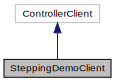
\includegraphics[width=188pt]{classSteppingDemoClient__inherit__graph}
\end{center}
\end{figure}


Collaboration diagram for Stepping\+Demo\+Client\+:\nopagebreak
\begin{figure}[H]
\begin{center}
\leavevmode
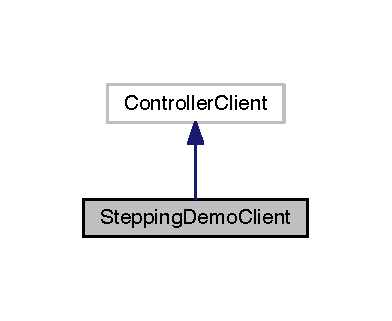
\includegraphics[width=188pt]{classSteppingDemoClient__coll__graph}
\end{center}
\end{figure}
\subsection*{Public Member Functions}
\begin{DoxyCompactItemize}
\item 
\hyperlink{classSteppingDemoClient_a28e41547ba5641741ceb3b378a5983db}{Stepping\+Demo\+Client} (std\+::shared\+\_\+ptr$<$ ocra\+::\+Model $>$ model\+Ptr, const int loop\+Period)
\item 
virtual \hyperlink{classSteppingDemoClient_a573eed904c7262c5cdbaf6e254d72559}{$\sim$\+Stepping\+Demo\+Client} ()
\end{DoxyCompactItemize}
\subsection*{Protected Member Functions}
\begin{DoxyCompactItemize}
\item 
virtual bool \hyperlink{classSteppingDemoClient_a08dce195eece162eed175ac9487667c2}{initialize} ()
\item 
virtual void \hyperlink{classSteppingDemoClient_aafcb227c0d7ce24823957e2331caa88b}{release} ()
\item 
virtual void \hyperlink{classSteppingDemoClient_a37dba4764b5849cf33c395cd0d4b0eb5}{loop} ()
\end{DoxyCompactItemize}
\subsection*{Private Member Functions}
\begin{DoxyCompactItemize}
\item 
Eigen\+::\+Vector3d \hyperlink{classSteppingDemoClient_af6a814243828f5136476aa5e99ea0079}{get\+Left\+Foot\+Position} ()
\item 
Eigen\+::\+Vector3d \hyperlink{classSteppingDemoClient_ae9c0d72756c109f49c269a7e1b06454a}{get\+Right\+Foot\+Position} ()
\item 
Eigen\+::\+Vector3d \hyperlink{classSteppingDemoClient_a857aa530a4ab94443d0b0869121baf76}{get\+Co\+M\+Position} ()
\item 
void \hyperlink{classSteppingDemoClient_a18609e5634a283423c228106bb0e3a45}{position\+Co\+M\+Over} (\hyperlink{SteppingDemoClient_8h_ac0c3848a609566394821d9826e0fdd5b}{C\+O\+M\+\_\+\+S\+U\+P\+P\+O\+R\+T\+\_\+\+P\+O\+S\+I\+T\+I\+ON} new\+Support\+Pos)
\item 
bool \hyperlink{classSteppingDemoClient_ad8fbc186267a47a73bb77e78199f2b8c}{is\+Balanced} ()
\item 
void \hyperlink{classSteppingDemoClient_a62b5028bdc99de117cfffc576478a0f1}{deactivate\+Foot\+Contacts} (\hyperlink{SteppingDemoClient_8h_ab0673d7f17cdd57b8fa124abb330287f}{F\+O\+O\+T\+\_\+\+C\+O\+N\+T\+A\+C\+TS} foot)
\item 
void \hyperlink{classSteppingDemoClient_abf583698c8c03620516acf3ec6eb9e41}{activate\+Foot\+Contacts} (\hyperlink{SteppingDemoClient_8h_ab0673d7f17cdd57b8fa124abb330287f}{F\+O\+O\+T\+\_\+\+C\+O\+N\+T\+A\+C\+TS} foot)
\item 
bool \hyperlink{classSteppingDemoClient_aeeaa9fac47e3e5a141647b07fa2feaa3}{is\+Foot\+In\+Contact} (\hyperlink{SteppingDemoClient_8h_ab0673d7f17cdd57b8fa124abb330287f}{F\+O\+O\+T\+\_\+\+C\+O\+N\+T\+A\+C\+TS} foot)
\item 
void \hyperlink{classSteppingDemoClient_a6b5d8bf0ce08c8b9f66ac2c1bbd5bcd7}{pause\+For} (double \+\_\+pause\+Duration)
\item 
bool \hyperlink{classSteppingDemoClient_afe78b799d8b8c63cff7d1e8765b7e1fa}{pause\+Finished} ()
\item 
bool \hyperlink{classSteppingDemoClient_a927c8615104a5fd5968ea4ece2c22926}{lift\+Foot} (\hyperlink{SteppingDemoClient_8h_ab0673d7f17cdd57b8fa124abb330287f}{F\+O\+O\+T\+\_\+\+C\+O\+N\+T\+A\+C\+TS} foot)
\item 
bool \hyperlink{classSteppingDemoClient_ae406e5c8f755f234272b63de4d6a774f}{lift\+Foot} (\hyperlink{SteppingDemoClient_8h_ab0673d7f17cdd57b8fa124abb330287f}{F\+O\+O\+T\+\_\+\+C\+O\+N\+T\+A\+C\+TS} foot, bool is\+Left\+Foot\+In\+Contact, bool is\+Right\+Foot\+In\+Contact)
\item 
bool \hyperlink{classSteppingDemoClient_a930123dad5658ea8a3bb5f23cb4cb369}{set\+Down\+Foot} (\hyperlink{SteppingDemoClient_8h_ab0673d7f17cdd57b8fa124abb330287f}{F\+O\+O\+T\+\_\+\+C\+O\+N\+T\+A\+C\+TS} foot)
\end{DoxyCompactItemize}
\subsection*{Private Attributes}
\begin{DoxyCompactItemize}
\item 
ocra\+\_\+recipes\+::\+Task\+Connection\+::\+Ptr \hyperlink{classSteppingDemoClient_a5dd71720cd8f7a17d21f74d20b3c23ff}{Left\+Foot\+Contact\+\_\+\+Back\+Left}
\item 
ocra\+\_\+recipes\+::\+Task\+Connection\+::\+Ptr \hyperlink{classSteppingDemoClient_a32e69816ec216b3d6502385e2346d22d}{Left\+Foot\+Contact\+\_\+\+Front\+Left}
\item 
ocra\+\_\+recipes\+::\+Task\+Connection\+::\+Ptr \hyperlink{classSteppingDemoClient_a946ab9de6d55274e5cb9b9a8743a30b8}{Left\+Foot\+Contact\+\_\+\+Back\+Right}
\item 
ocra\+\_\+recipes\+::\+Task\+Connection\+::\+Ptr \hyperlink{classSteppingDemoClient_ae2c0ca1ba0ef69b5f09fd3cd982fb772}{Left\+Foot\+Contact\+\_\+\+Front\+Right}
\item 
ocra\+\_\+recipes\+::\+Task\+Connection\+::\+Ptr \hyperlink{classSteppingDemoClient_aaaf5dee15bf151def4b4070751d1ca84}{Right\+Foot\+Contact\+\_\+\+Back\+Left}
\item 
ocra\+\_\+recipes\+::\+Task\+Connection\+::\+Ptr \hyperlink{classSteppingDemoClient_ad10f639e025b003fd383f4cc933da15f}{Right\+Foot\+Contact\+\_\+\+Front\+Left}
\item 
ocra\+\_\+recipes\+::\+Task\+Connection\+::\+Ptr \hyperlink{classSteppingDemoClient_a93e209732588c3ef2b04e39e3df40d3e}{Right\+Foot\+Contact\+\_\+\+Back\+Right}
\item 
ocra\+\_\+recipes\+::\+Task\+Connection\+::\+Ptr \hyperlink{classSteppingDemoClient_a781be1c0ffd7e7147eb2b2de66ba3231}{Right\+Foot\+Contact\+\_\+\+Front\+Right}
\item 
double \hyperlink{classSteppingDemoClient_a13a5deff16d52936f788bb9b0af6e9c9}{pause\+Trigger\+Time}
\item 
double \hyperlink{classSteppingDemoClient_a92b810b2d2c50e359da18e5d91163340}{pause\+Duration}
\item 
double \hyperlink{classSteppingDemoClient_a1bb7d42cf09778349ae1ecd31d2ac116}{current\+Time}
\item 
bool \hyperlink{classSteppingDemoClient_a29e7765300c7d2e2d5108025fbdcbc2c}{is\+Pausing}
\item 
bool \hyperlink{classSteppingDemoClient_a88b84ed8fc7808ea3fb68f2ec3d29ebe}{is\+In\+Left\+Support\+Mode}
\item 
bool \hyperlink{classSteppingDemoClient_a7697070e5db6c635aa2eff70bce29176}{is\+In\+Right\+Support\+Mode}
\item 
bool \hyperlink{classSteppingDemoClient_a6036e2d0b604648ca39e4d64b41a9d6e}{foot\+Trajectory\+Started}
\item 
std\+::shared\+\_\+ptr$<$ ocra\+\_\+recipes\+::\+Trajectory\+Thread $>$ \hyperlink{classSteppingDemoClient_afd18627088c2c12f172ff9e976da5330}{left\+Foot\+\_\+\+Traj\+Thread}
\item 
std\+::shared\+\_\+ptr$<$ ocra\+\_\+recipes\+::\+Trajectory\+Thread $>$ \hyperlink{classSteppingDemoClient_a8b4b931d41b47d9923417506fac107f3}{right\+Foot\+\_\+\+Traj\+Thread}
\item 
std\+::shared\+\_\+ptr$<$ ocra\+\_\+recipes\+::\+Trajectory\+Thread $>$ \hyperlink{classSteppingDemoClient_a9f3d1cdc49cc26a10f9b8fb0d0c68cab}{com\+\_\+\+Traj\+Thread}
\item 
Eigen\+::\+Vector3d \hyperlink{classSteppingDemoClient_acd4cb9dbe053979701574f5d1d4ef349}{left\+Foot\+Home}
\item 
Eigen\+::\+Vector3d \hyperlink{classSteppingDemoClient_ae2a3bdaafc7784b5afece8ae9ebaff7d}{right\+Foot\+Home}
\item 
Eigen\+::\+Vector3d \hyperlink{classSteppingDemoClient_aa018c1f2734d63f962be512461c9e010}{com\+Home}
\item 
Eigen\+::\+Vector3d \hyperlink{classSteppingDemoClient_a2360933e2902d1b1a374787bd67e14e7}{left\+Foot\+Target}
\item 
Eigen\+::\+Vector3d \hyperlink{classSteppingDemoClient_abfe6635a0ad50fa4baa6fa10b8c56d9e}{right\+Foot\+Target}
\item 
Eigen\+::\+Vector3d \hyperlink{classSteppingDemoClient_ab4a77111abbf3630280a64d17ac59eef}{new\+Co\+M\+Goal\+Position}
\item 
double \hyperlink{classSteppingDemoClient_af7b6e48319ef9d35fb975edc3bb2a137}{start\+Time}
\item 
bool \hyperlink{classSteppingDemoClient_aedd8bb5bca60afbdd2b8de3b5d1829d7}{get\+Initial\+Values}
\item 
\hyperlink{SteppingDemoClient_8h_af2a8507bf21c3ce9b0e67a23381251c6}{C\+O\+N\+T\+R\+O\+L\+\_\+\+P\+H\+A\+SE} \hyperlink{classSteppingDemoClient_afe0aa2a02ea8117d644bf5444a03ac62}{current\+Phase}
\item 
\hyperlink{SteppingDemoClient_8h_af2a8507bf21c3ce9b0e67a23381251c6}{C\+O\+N\+T\+R\+O\+L\+\_\+\+P\+H\+A\+SE} \hyperlink{classSteppingDemoClient_ab5a3b82049a9786162a60d0ae94f96d9}{next\+Phase}
\item 
bool \hyperlink{classSteppingDemoClient_ad7e3950d053af7c1aca33b3e7c3b20c5}{is\+Moving\+CoM}
\end{DoxyCompactItemize}


\subsection{Constructor \& Destructor Documentation}
\hypertarget{classSteppingDemoClient_a28e41547ba5641741ceb3b378a5983db}{}\label{classSteppingDemoClient_a28e41547ba5641741ceb3b378a5983db} 
\index{Stepping\+Demo\+Client@{Stepping\+Demo\+Client}!Stepping\+Demo\+Client@{Stepping\+Demo\+Client}}
\index{Stepping\+Demo\+Client@{Stepping\+Demo\+Client}!Stepping\+Demo\+Client@{Stepping\+Demo\+Client}}
\subsubsection{\texorpdfstring{Stepping\+Demo\+Client()}{SteppingDemoClient()}}
{\footnotesize\ttfamily Stepping\+Demo\+Client\+::\+Stepping\+Demo\+Client (\begin{DoxyParamCaption}\item[{std\+::shared\+\_\+ptr$<$ ocra\+::\+Model $>$}]{model\+Ptr,  }\item[{const int}]{loop\+Period }\end{DoxyParamCaption})}

\hypertarget{classSteppingDemoClient_a573eed904c7262c5cdbaf6e254d72559}{}\label{classSteppingDemoClient_a573eed904c7262c5cdbaf6e254d72559} 
\index{Stepping\+Demo\+Client@{Stepping\+Demo\+Client}!````~Stepping\+Demo\+Client@{$\sim$\+Stepping\+Demo\+Client}}
\index{````~Stepping\+Demo\+Client@{$\sim$\+Stepping\+Demo\+Client}!Stepping\+Demo\+Client@{Stepping\+Demo\+Client}}
\subsubsection{\texorpdfstring{$\sim$\+Stepping\+Demo\+Client()}{~SteppingDemoClient()}}
{\footnotesize\ttfamily Stepping\+Demo\+Client\+::$\sim$\+Stepping\+Demo\+Client (\begin{DoxyParamCaption}{ }\end{DoxyParamCaption})\hspace{0.3cm}{\ttfamily [virtual]}}



\subsection{Member Function Documentation}
\hypertarget{classSteppingDemoClient_abf583698c8c03620516acf3ec6eb9e41}{}\label{classSteppingDemoClient_abf583698c8c03620516acf3ec6eb9e41} 
\index{Stepping\+Demo\+Client@{Stepping\+Demo\+Client}!activate\+Foot\+Contacts@{activate\+Foot\+Contacts}}
\index{activate\+Foot\+Contacts@{activate\+Foot\+Contacts}!Stepping\+Demo\+Client@{Stepping\+Demo\+Client}}
\subsubsection{\texorpdfstring{activate\+Foot\+Contacts()}{activateFootContacts()}}
{\footnotesize\ttfamily void Stepping\+Demo\+Client\+::activate\+Foot\+Contacts (\begin{DoxyParamCaption}\item[{\hyperlink{SteppingDemoClient_8h_ab0673d7f17cdd57b8fa124abb330287f}{F\+O\+O\+T\+\_\+\+C\+O\+N\+T\+A\+C\+TS}}]{foot }\end{DoxyParamCaption})\hspace{0.3cm}{\ttfamily [private]}}

This method asks the ocra-\/icub-\/server to activate one by one the feet \char`\"{}corner\char`\"{} contact tasks for the specified foot.


\begin{DoxyParams}{Parameters}
{\em foot} & L\+E\+F\+T\+\_\+\+F\+O\+OT or R\+I\+G\+H\+T\+\_\+\+F\+O\+OT. \\
\hline
\end{DoxyParams}
\hypertarget{classSteppingDemoClient_a62b5028bdc99de117cfffc576478a0f1}{}\label{classSteppingDemoClient_a62b5028bdc99de117cfffc576478a0f1} 
\index{Stepping\+Demo\+Client@{Stepping\+Demo\+Client}!deactivate\+Foot\+Contacts@{deactivate\+Foot\+Contacts}}
\index{deactivate\+Foot\+Contacts@{deactivate\+Foot\+Contacts}!Stepping\+Demo\+Client@{Stepping\+Demo\+Client}}
\subsubsection{\texorpdfstring{deactivate\+Foot\+Contacts()}{deactivateFootContacts()}}
{\footnotesize\ttfamily void Stepping\+Demo\+Client\+::deactivate\+Foot\+Contacts (\begin{DoxyParamCaption}\item[{\hyperlink{SteppingDemoClient_8h_ab0673d7f17cdd57b8fa124abb330287f}{F\+O\+O\+T\+\_\+\+C\+O\+N\+T\+A\+C\+TS}}]{foot }\end{DoxyParamCaption})\hspace{0.3cm}{\ttfamily [private]}}

Remember the right and left feet contact tasks? created in \hyperlink{classSteppingDemoClient_a08dce195eece162eed175ac9487667c2}{initialize()}. This method acts the ocra-\/icub-\/server to deactivate one by one the feet \char`\"{}corner\char`\"{} contact tasks for the specified foot.


\begin{DoxyParams}{Parameters}
{\em foot} & L\+E\+F\+T\+\_\+\+F\+O\+OT or R\+I\+G\+H\+T\+\_\+\+F\+O\+OT. \\
\hline
\end{DoxyParams}
\hypertarget{classSteppingDemoClient_a857aa530a4ab94443d0b0869121baf76}{}\label{classSteppingDemoClient_a857aa530a4ab94443d0b0869121baf76} 
\index{Stepping\+Demo\+Client@{Stepping\+Demo\+Client}!get\+Co\+M\+Position@{get\+Co\+M\+Position}}
\index{get\+Co\+M\+Position@{get\+Co\+M\+Position}!Stepping\+Demo\+Client@{Stepping\+Demo\+Client}}
\subsubsection{\texorpdfstring{get\+Co\+M\+Position()}{getCoMPosition()}}
{\footnotesize\ttfamily Eigen\+::\+Vector3d Stepping\+Demo\+Client\+::get\+Co\+M\+Position (\begin{DoxyParamCaption}{ }\end{DoxyParamCaption})\hspace{0.3cm}{\ttfamily [private]}}

Retrieves the 3D position of the \char`\"{}\+Co\+M\char`\"{} as done by the yarp\+Whole\+Body\+Interface.

\begin{DoxyReturn}{Returns}
3D position of the C\+OM. 
\end{DoxyReturn}
\hypertarget{classSteppingDemoClient_af6a814243828f5136476aa5e99ea0079}{}\label{classSteppingDemoClient_af6a814243828f5136476aa5e99ea0079} 
\index{Stepping\+Demo\+Client@{Stepping\+Demo\+Client}!get\+Left\+Foot\+Position@{get\+Left\+Foot\+Position}}
\index{get\+Left\+Foot\+Position@{get\+Left\+Foot\+Position}!Stepping\+Demo\+Client@{Stepping\+Demo\+Client}}
\subsubsection{\texorpdfstring{get\+Left\+Foot\+Position()}{getLeftFootPosition()}}
{\footnotesize\ttfamily Eigen\+::\+Vector3d Stepping\+Demo\+Client\+::get\+Left\+Foot\+Position (\begin{DoxyParamCaption}{ }\end{DoxyParamCaption})\hspace{0.3cm}{\ttfamily [private]}}

Retrieves the 3D position of the \char`\"{}l\+\_\+sole\char`\"{} frame from the i\+Cub model.

\begin{DoxyReturn}{Returns}
3D position of the left foot. 
\end{DoxyReturn}
\hypertarget{classSteppingDemoClient_ae9c0d72756c109f49c269a7e1b06454a}{}\label{classSteppingDemoClient_ae9c0d72756c109f49c269a7e1b06454a} 
\index{Stepping\+Demo\+Client@{Stepping\+Demo\+Client}!get\+Right\+Foot\+Position@{get\+Right\+Foot\+Position}}
\index{get\+Right\+Foot\+Position@{get\+Right\+Foot\+Position}!Stepping\+Demo\+Client@{Stepping\+Demo\+Client}}
\subsubsection{\texorpdfstring{get\+Right\+Foot\+Position()}{getRightFootPosition()}}
{\footnotesize\ttfamily Eigen\+::\+Vector3d Stepping\+Demo\+Client\+::get\+Right\+Foot\+Position (\begin{DoxyParamCaption}{ }\end{DoxyParamCaption})\hspace{0.3cm}{\ttfamily [private]}}

Retrieves the 3D position of the \char`\"{}r\+\_\+sole\char`\"{} frame from the i\+Cub model.

\begin{DoxyReturn}{Returns}
3D position of the right foot. 
\end{DoxyReturn}
\hypertarget{classSteppingDemoClient_a08dce195eece162eed175ac9487667c2}{}\label{classSteppingDemoClient_a08dce195eece162eed175ac9487667c2} 
\index{Stepping\+Demo\+Client@{Stepping\+Demo\+Client}!initialize@{initialize}}
\index{initialize@{initialize}!Stepping\+Demo\+Client@{Stepping\+Demo\+Client}}
\subsubsection{\texorpdfstring{initialize()}{initialize()}}
{\footnotesize\ttfamily bool Stepping\+Demo\+Client\+::initialize (\begin{DoxyParamCaption}{ }\end{DoxyParamCaption})\hspace{0.3cm}{\ttfamily [protected]}, {\ttfamily [virtual]}}

The initialization consists of the following\+:
\begin{DoxyEnumerate}
\item Defines trajectory types (e.\+g. Min. Jerk)
\item Defines the termination strategy
\item Instantiates trajectory threads for the left and right foot as well as for the CoM, sets them up (max velocity, error threshold) and finally starts them.
\item Instantiates ocra\+::\+Task\+Connection objects for the left and right feet contacts (4 per foot on each corner).
\end{DoxyEnumerate}
\begin{DoxyItemize}
\item returns\+: True if everything has been initialized properly, false otherwise. 
\end{DoxyItemize}\hypertarget{classSteppingDemoClient_ad8fbc186267a47a73bb77e78199f2b8c}{}\label{classSteppingDemoClient_ad8fbc186267a47a73bb77e78199f2b8c} 
\index{Stepping\+Demo\+Client@{Stepping\+Demo\+Client}!is\+Balanced@{is\+Balanced}}
\index{is\+Balanced@{is\+Balanced}!Stepping\+Demo\+Client@{Stepping\+Demo\+Client}}
\subsubsection{\texorpdfstring{is\+Balanced()}{isBalanced()}}
{\footnotesize\ttfamily bool Stepping\+Demo\+Client\+::is\+Balanced (\begin{DoxyParamCaption}{ }\end{DoxyParamCaption})\hspace{0.3cm}{\ttfamily [private]}}

Uses the norm of the C\+OM and joint velocities to understand if the robot is balanced.

\begin{DoxyReturn}{Returns}
True when both the norm of the C\+OM and joint velocities are below com\+Vel\+Threshold and joint\+Threshold. 
\end{DoxyReturn}
\begin{DoxyRefDesc}{Todo}
\item[\hyperlink{todo__todo000002}{Todo}]A more balance-\/centered criterion should be used for this, Z\+M\+P-\/based for example. \end{DoxyRefDesc}
\hypertarget{classSteppingDemoClient_aeeaa9fac47e3e5a141647b07fa2feaa3}{}\label{classSteppingDemoClient_aeeaa9fac47e3e5a141647b07fa2feaa3} 
\index{Stepping\+Demo\+Client@{Stepping\+Demo\+Client}!is\+Foot\+In\+Contact@{is\+Foot\+In\+Contact}}
\index{is\+Foot\+In\+Contact@{is\+Foot\+In\+Contact}!Stepping\+Demo\+Client@{Stepping\+Demo\+Client}}
\subsubsection{\texorpdfstring{is\+Foot\+In\+Contact()}{isFootInContact()}}
{\footnotesize\ttfamily bool Stepping\+Demo\+Client\+::is\+Foot\+In\+Contact (\begin{DoxyParamCaption}\item[{\hyperlink{SteppingDemoClient_8h_ab0673d7f17cdd57b8fa124abb330287f}{F\+O\+O\+T\+\_\+\+C\+O\+N\+T\+A\+C\+TS}}]{foot }\end{DoxyParamCaption})\hspace{0.3cm}{\ttfamily [private]}}

If the foot height is less than or equal to foot\+Contact\+Release\+Threshold, the feet contacts tasks are activated.


\begin{DoxyParams}{Parameters}
{\em foot} & L\+E\+F\+T\+\_\+\+F\+O\+OT or R\+I\+G\+H\+T\+\_\+\+F\+O\+OT.\\
\hline
\end{DoxyParams}
\begin{DoxyReturn}{Returns}
True if the activation of the contact happens successfully. False if the foot\textquotesingle{}s elevation is not under the foot\+Contact\+Release\+Threshold. 
\end{DoxyReturn}
\hypertarget{classSteppingDemoClient_a927c8615104a5fd5968ea4ece2c22926}{}\label{classSteppingDemoClient_a927c8615104a5fd5968ea4ece2c22926} 
\index{Stepping\+Demo\+Client@{Stepping\+Demo\+Client}!lift\+Foot@{lift\+Foot}}
\index{lift\+Foot@{lift\+Foot}!Stepping\+Demo\+Client@{Stepping\+Demo\+Client}}
\subsubsection{\texorpdfstring{lift\+Foot()}{liftFoot()}\hspace{0.1cm}{\footnotesize\ttfamily [1/2]}}
{\footnotesize\ttfamily bool Stepping\+Demo\+Client\+::lift\+Foot (\begin{DoxyParamCaption}\item[{\hyperlink{SteppingDemoClient_8h_ab0673d7f17cdd57b8fa124abb330287f}{F\+O\+O\+T\+\_\+\+C\+O\+N\+T\+A\+C\+TS}}]{foot }\end{DoxyParamCaption})\hspace{0.3cm}{\ttfamily [private]}}

Sets the right or left foot waypoint to right\+Foot\+Target or left\+Foot\+Target accordingly (where the foot will be lifted). These values are harcoded in the \hyperlink{classSteppingDemoClient_a37dba4764b5849cf33c395cd0d4b0eb5}{loop()} method and updated only during the very first iteration when the variable get\+Initial\+Values is set to true.


\begin{DoxyParams}{Parameters}
{\em foot} & L\+E\+F\+T\+\_\+\+F\+O\+OT or R\+I\+G\+H\+T\+\_\+\+F\+O\+OT\\
\hline
\end{DoxyParams}
\begin{DoxyReturn}{Returns}
True after the foot contact is deactivated. 
\end{DoxyReturn}
\hypertarget{classSteppingDemoClient_ae406e5c8f755f234272b63de4d6a774f}{}\label{classSteppingDemoClient_ae406e5c8f755f234272b63de4d6a774f} 
\index{Stepping\+Demo\+Client@{Stepping\+Demo\+Client}!lift\+Foot@{lift\+Foot}}
\index{lift\+Foot@{lift\+Foot}!Stepping\+Demo\+Client@{Stepping\+Demo\+Client}}
\subsubsection{\texorpdfstring{lift\+Foot()}{liftFoot()}\hspace{0.1cm}{\footnotesize\ttfamily [2/2]}}
{\footnotesize\ttfamily bool Stepping\+Demo\+Client\+::lift\+Foot (\begin{DoxyParamCaption}\item[{\hyperlink{SteppingDemoClient_8h_ab0673d7f17cdd57b8fa124abb330287f}{F\+O\+O\+T\+\_\+\+C\+O\+N\+T\+A\+C\+TS}}]{foot,  }\item[{bool}]{is\+Left\+Foot\+In\+Contact,  }\item[{bool}]{is\+Right\+Foot\+In\+Contact }\end{DoxyParamCaption})\hspace{0.3cm}{\ttfamily [private]}}

Sets the right or left foot waypoint to right\+Foot\+Target or left\+Foot\+Target accordingly (where the foot will be lifted). These values are harcoded in the \hyperlink{classSteppingDemoClient_a37dba4764b5849cf33c395cd0d4b0eb5}{loop()} method and updated only during the very first iteration when the variable get\+Initial\+Values is set to true.


\begin{DoxyParams}{Parameters}
{\em foot} & L\+E\+F\+T\+\_\+\+F\+O\+OT or R\+I\+G\+H\+T\+\_\+\+F\+O\+OT \\
\hline
{\em is\+Left\+Foot\+In\+Contact} & Updates the current state of the left foot contact. \\
\hline
{\em is\+Right\+Foot\+In\+Contact} & Updates the current state of the right foot contact.\\
\hline
\end{DoxyParams}
\begin{DoxyReturn}{Returns}
True after the foot contact is deactivated. 
\end{DoxyReturn}
\hypertarget{classSteppingDemoClient_a37dba4764b5849cf33c395cd0d4b0eb5}{}\label{classSteppingDemoClient_a37dba4764b5849cf33c395cd0d4b0eb5} 
\index{Stepping\+Demo\+Client@{Stepping\+Demo\+Client}!loop@{loop}}
\index{loop@{loop}!Stepping\+Demo\+Client@{Stepping\+Demo\+Client}}
\subsubsection{\texorpdfstring{loop()}{loop()}}
{\footnotesize\ttfamily void Stepping\+Demo\+Client\+::loop (\begin{DoxyParamCaption}{ }\end{DoxyParamCaption})\hspace{0.3cm}{\ttfamily [protected]}, {\ttfamily [virtual]}}

Initially waits for two seconds, to make sure that all model states have been correctly updated during the initialization. During the first loop it retrieves left and right feet positions along with the com\textquotesingle{}s. \hypertarget{classSteppingDemoClient_afe78b799d8b8c63cff7d1e8765b7e1fa}{}\label{classSteppingDemoClient_afe78b799d8b8c63cff7d1e8765b7e1fa} 
\index{Stepping\+Demo\+Client@{Stepping\+Demo\+Client}!pause\+Finished@{pause\+Finished}}
\index{pause\+Finished@{pause\+Finished}!Stepping\+Demo\+Client@{Stepping\+Demo\+Client}}
\subsubsection{\texorpdfstring{pause\+Finished()}{pauseFinished()}}
{\footnotesize\ttfamily bool Stepping\+Demo\+Client\+::pause\+Finished (\begin{DoxyParamCaption}{ }\end{DoxyParamCaption})\hspace{0.3cm}{\ttfamily [private]}}

Sets is\+Pausing to false when pause\+Duration has passed.

\begin{DoxyReturn}{Returns}
True when the pause duration is over. False otherwise. 
\end{DoxyReturn}
\hypertarget{classSteppingDemoClient_a6b5d8bf0ce08c8b9f66ac2c1bbd5bcd7}{}\label{classSteppingDemoClient_a6b5d8bf0ce08c8b9f66ac2c1bbd5bcd7} 
\index{Stepping\+Demo\+Client@{Stepping\+Demo\+Client}!pause\+For@{pause\+For}}
\index{pause\+For@{pause\+For}!Stepping\+Demo\+Client@{Stepping\+Demo\+Client}}
\subsubsection{\texorpdfstring{pause\+For()}{pauseFor()}}
{\footnotesize\ttfamily void Stepping\+Demo\+Client\+::pause\+For (\begin{DoxyParamCaption}\item[{double}]{\+\_\+pause\+Duration }\end{DoxyParamCaption})\hspace{0.3cm}{\ttfamily [private]}}

Mainly sets is\+Pausing to true and stores the time at which the pause was called.


\begin{DoxyParams}{Parameters}
{\em \+\_\+pause\+Duration} & Pause duration. \\
\hline
\end{DoxyParams}
\hypertarget{classSteppingDemoClient_a18609e5634a283423c228106bb0e3a45}{}\label{classSteppingDemoClient_a18609e5634a283423c228106bb0e3a45} 
\index{Stepping\+Demo\+Client@{Stepping\+Demo\+Client}!position\+Co\+M\+Over@{position\+Co\+M\+Over}}
\index{position\+Co\+M\+Over@{position\+Co\+M\+Over}!Stepping\+Demo\+Client@{Stepping\+Demo\+Client}}
\subsubsection{\texorpdfstring{position\+Co\+M\+Over()}{positionCoMOver()}}
{\footnotesize\ttfamily void Stepping\+Demo\+Client\+::position\+Co\+M\+Over (\begin{DoxyParamCaption}\item[{\hyperlink{SteppingDemoClient_8h_ac0c3848a609566394821d9826e0fdd5b}{C\+O\+M\+\_\+\+S\+U\+P\+P\+O\+R\+T\+\_\+\+P\+O\+S\+I\+T\+I\+ON}}]{new\+Support\+Pos }\end{DoxyParamCaption})\hspace{0.3cm}{\ttfamily [private]}}

Sets C\+OM trajectory waypoints according to the desired support position\+: L\+E\+F\+T\+\_\+\+F\+O\+O\+T\+\_\+\+XY\+: The C\+OM goal position is set to be on top of the left foot. R\+I\+G\+H\+T\+\_\+\+F\+O\+O\+T\+\_\+\+XY\+: The C\+OM goal position is set to be on top of the right foot. C\+E\+N\+T\+E\+R\+E\+D\+\_\+\+B\+E\+T\+W\+E\+E\+N\+\_\+\+F\+E\+E\+T\+\_\+\+XY\+: The C\+OM goal position is set between both feet. The height of the com is always the current C\+OM\textquotesingle{}s height. Since the thread must have started before calling this method, it will update the current waypoint trajectory it has or start it.


\begin{DoxyParams}{Parameters}
{\em new\+Support\+Pos} & New support position. \\
\hline
\end{DoxyParams}
\hypertarget{classSteppingDemoClient_aafcb227c0d7ce24823957e2331caa88b}{}\label{classSteppingDemoClient_aafcb227c0d7ce24823957e2331caa88b} 
\index{Stepping\+Demo\+Client@{Stepping\+Demo\+Client}!release@{release}}
\index{release@{release}!Stepping\+Demo\+Client@{Stepping\+Demo\+Client}}
\subsubsection{\texorpdfstring{release()}{release()}}
{\footnotesize\ttfamily void Stepping\+Demo\+Client\+::release (\begin{DoxyParamCaption}{ }\end{DoxyParamCaption})\hspace{0.3cm}{\ttfamily [protected]}, {\ttfamily [virtual]}}

Stops the trajectory threads of the CoM, left and right feet. \hypertarget{classSteppingDemoClient_a930123dad5658ea8a3bb5f23cb4cb369}{}\label{classSteppingDemoClient_a930123dad5658ea8a3bb5f23cb4cb369} 
\index{Stepping\+Demo\+Client@{Stepping\+Demo\+Client}!set\+Down\+Foot@{set\+Down\+Foot}}
\index{set\+Down\+Foot@{set\+Down\+Foot}!Stepping\+Demo\+Client@{Stepping\+Demo\+Client}}
\subsubsection{\texorpdfstring{set\+Down\+Foot()}{setDownFoot()}}
{\footnotesize\ttfamily bool Stepping\+Demo\+Client\+::set\+Down\+Foot (\begin{DoxyParamCaption}\item[{\hyperlink{SteppingDemoClient_8h_ab0673d7f17cdd57b8fa124abb330287f}{F\+O\+O\+T\+\_\+\+C\+O\+N\+T\+A\+C\+TS}}]{foot }\end{DoxyParamCaption})\hspace{0.3cm}{\ttfamily [private]}}

Sets the right or left foot waypoint to right\+Foot\+Home or left\+Foot\+Home accordingly (where the foot will land). These values are harcoded in the \hyperlink{classSteppingDemoClient_a37dba4764b5849cf33c395cd0d4b0eb5}{loop()} method and updated only during the very first iteration when the variable get\+Initial\+Values is set to true.


\begin{DoxyParams}{Parameters}
{\em foot} & L\+E\+F\+T\+\_\+\+F\+O\+OT or R\+I\+G\+H\+T\+\_\+\+F\+O\+OT\\
\hline
\end{DoxyParams}
\begin{DoxyReturn}{Returns}
True only after the foot has established contact again and the trajectory is over. False while the foot is still moving back down looking for contact or simply, the goal hasn\textquotesingle{}t been attained. 
\end{DoxyReturn}


\subsection{Member Data Documentation}
\hypertarget{classSteppingDemoClient_a9f3d1cdc49cc26a10f9b8fb0d0c68cab}{}\label{classSteppingDemoClient_a9f3d1cdc49cc26a10f9b8fb0d0c68cab} 
\index{Stepping\+Demo\+Client@{Stepping\+Demo\+Client}!com\+\_\+\+Traj\+Thread@{com\+\_\+\+Traj\+Thread}}
\index{com\+\_\+\+Traj\+Thread@{com\+\_\+\+Traj\+Thread}!Stepping\+Demo\+Client@{Stepping\+Demo\+Client}}
\subsubsection{\texorpdfstring{com\+\_\+\+Traj\+Thread}{com\_TrajThread}}
{\footnotesize\ttfamily std\+::shared\+\_\+ptr$<$ocra\+\_\+recipes\+::\+Trajectory\+Thread$>$ Stepping\+Demo\+Client\+::com\+\_\+\+Traj\+Thread\hspace{0.3cm}{\ttfamily [private]}}

\hypertarget{classSteppingDemoClient_aa018c1f2734d63f962be512461c9e010}{}\label{classSteppingDemoClient_aa018c1f2734d63f962be512461c9e010} 
\index{Stepping\+Demo\+Client@{Stepping\+Demo\+Client}!com\+Home@{com\+Home}}
\index{com\+Home@{com\+Home}!Stepping\+Demo\+Client@{Stepping\+Demo\+Client}}
\subsubsection{\texorpdfstring{com\+Home}{comHome}}
{\footnotesize\ttfamily Eigen\+::\+Vector3d Stepping\+Demo\+Client\+::com\+Home\hspace{0.3cm}{\ttfamily [private]}}

\hypertarget{classSteppingDemoClient_afe0aa2a02ea8117d644bf5444a03ac62}{}\label{classSteppingDemoClient_afe0aa2a02ea8117d644bf5444a03ac62} 
\index{Stepping\+Demo\+Client@{Stepping\+Demo\+Client}!current\+Phase@{current\+Phase}}
\index{current\+Phase@{current\+Phase}!Stepping\+Demo\+Client@{Stepping\+Demo\+Client}}
\subsubsection{\texorpdfstring{current\+Phase}{currentPhase}}
{\footnotesize\ttfamily \hyperlink{SteppingDemoClient_8h_af2a8507bf21c3ce9b0e67a23381251c6}{C\+O\+N\+T\+R\+O\+L\+\_\+\+P\+H\+A\+SE} Stepping\+Demo\+Client\+::current\+Phase\hspace{0.3cm}{\ttfamily [private]}}

\hypertarget{classSteppingDemoClient_a1bb7d42cf09778349ae1ecd31d2ac116}{}\label{classSteppingDemoClient_a1bb7d42cf09778349ae1ecd31d2ac116} 
\index{Stepping\+Demo\+Client@{Stepping\+Demo\+Client}!current\+Time@{current\+Time}}
\index{current\+Time@{current\+Time}!Stepping\+Demo\+Client@{Stepping\+Demo\+Client}}
\subsubsection{\texorpdfstring{current\+Time}{currentTime}}
{\footnotesize\ttfamily double Stepping\+Demo\+Client\+::current\+Time\hspace{0.3cm}{\ttfamily [private]}}

\hypertarget{classSteppingDemoClient_a6036e2d0b604648ca39e4d64b41a9d6e}{}\label{classSteppingDemoClient_a6036e2d0b604648ca39e4d64b41a9d6e} 
\index{Stepping\+Demo\+Client@{Stepping\+Demo\+Client}!foot\+Trajectory\+Started@{foot\+Trajectory\+Started}}
\index{foot\+Trajectory\+Started@{foot\+Trajectory\+Started}!Stepping\+Demo\+Client@{Stepping\+Demo\+Client}}
\subsubsection{\texorpdfstring{foot\+Trajectory\+Started}{footTrajectoryStarted}}
{\footnotesize\ttfamily bool Stepping\+Demo\+Client\+::foot\+Trajectory\+Started\hspace{0.3cm}{\ttfamily [private]}}

\hypertarget{classSteppingDemoClient_aedd8bb5bca60afbdd2b8de3b5d1829d7}{}\label{classSteppingDemoClient_aedd8bb5bca60afbdd2b8de3b5d1829d7} 
\index{Stepping\+Demo\+Client@{Stepping\+Demo\+Client}!get\+Initial\+Values@{get\+Initial\+Values}}
\index{get\+Initial\+Values@{get\+Initial\+Values}!Stepping\+Demo\+Client@{Stepping\+Demo\+Client}}
\subsubsection{\texorpdfstring{get\+Initial\+Values}{getInitialValues}}
{\footnotesize\ttfamily bool Stepping\+Demo\+Client\+::get\+Initial\+Values\hspace{0.3cm}{\ttfamily [private]}}

\hypertarget{classSteppingDemoClient_a88b84ed8fc7808ea3fb68f2ec3d29ebe}{}\label{classSteppingDemoClient_a88b84ed8fc7808ea3fb68f2ec3d29ebe} 
\index{Stepping\+Demo\+Client@{Stepping\+Demo\+Client}!is\+In\+Left\+Support\+Mode@{is\+In\+Left\+Support\+Mode}}
\index{is\+In\+Left\+Support\+Mode@{is\+In\+Left\+Support\+Mode}!Stepping\+Demo\+Client@{Stepping\+Demo\+Client}}
\subsubsection{\texorpdfstring{is\+In\+Left\+Support\+Mode}{isInLeftSupportMode}}
{\footnotesize\ttfamily bool Stepping\+Demo\+Client\+::is\+In\+Left\+Support\+Mode\hspace{0.3cm}{\ttfamily [private]}}

\hypertarget{classSteppingDemoClient_a7697070e5db6c635aa2eff70bce29176}{}\label{classSteppingDemoClient_a7697070e5db6c635aa2eff70bce29176} 
\index{Stepping\+Demo\+Client@{Stepping\+Demo\+Client}!is\+In\+Right\+Support\+Mode@{is\+In\+Right\+Support\+Mode}}
\index{is\+In\+Right\+Support\+Mode@{is\+In\+Right\+Support\+Mode}!Stepping\+Demo\+Client@{Stepping\+Demo\+Client}}
\subsubsection{\texorpdfstring{is\+In\+Right\+Support\+Mode}{isInRightSupportMode}}
{\footnotesize\ttfamily bool Stepping\+Demo\+Client\+::is\+In\+Right\+Support\+Mode\hspace{0.3cm}{\ttfamily [private]}}

\hypertarget{classSteppingDemoClient_ad7e3950d053af7c1aca33b3e7c3b20c5}{}\label{classSteppingDemoClient_ad7e3950d053af7c1aca33b3e7c3b20c5} 
\index{Stepping\+Demo\+Client@{Stepping\+Demo\+Client}!is\+Moving\+CoM@{is\+Moving\+CoM}}
\index{is\+Moving\+CoM@{is\+Moving\+CoM}!Stepping\+Demo\+Client@{Stepping\+Demo\+Client}}
\subsubsection{\texorpdfstring{is\+Moving\+CoM}{isMovingCoM}}
{\footnotesize\ttfamily bool Stepping\+Demo\+Client\+::is\+Moving\+CoM\hspace{0.3cm}{\ttfamily [private]}}

\hypertarget{classSteppingDemoClient_a29e7765300c7d2e2d5108025fbdcbc2c}{}\label{classSteppingDemoClient_a29e7765300c7d2e2d5108025fbdcbc2c} 
\index{Stepping\+Demo\+Client@{Stepping\+Demo\+Client}!is\+Pausing@{is\+Pausing}}
\index{is\+Pausing@{is\+Pausing}!Stepping\+Demo\+Client@{Stepping\+Demo\+Client}}
\subsubsection{\texorpdfstring{is\+Pausing}{isPausing}}
{\footnotesize\ttfamily bool Stepping\+Demo\+Client\+::is\+Pausing\hspace{0.3cm}{\ttfamily [private]}}

\hypertarget{classSteppingDemoClient_afd18627088c2c12f172ff9e976da5330}{}\label{classSteppingDemoClient_afd18627088c2c12f172ff9e976da5330} 
\index{Stepping\+Demo\+Client@{Stepping\+Demo\+Client}!left\+Foot\+\_\+\+Traj\+Thread@{left\+Foot\+\_\+\+Traj\+Thread}}
\index{left\+Foot\+\_\+\+Traj\+Thread@{left\+Foot\+\_\+\+Traj\+Thread}!Stepping\+Demo\+Client@{Stepping\+Demo\+Client}}
\subsubsection{\texorpdfstring{left\+Foot\+\_\+\+Traj\+Thread}{leftFoot\_TrajThread}}
{\footnotesize\ttfamily std\+::shared\+\_\+ptr$<$ocra\+\_\+recipes\+::\+Trajectory\+Thread$>$ Stepping\+Demo\+Client\+::left\+Foot\+\_\+\+Traj\+Thread\hspace{0.3cm}{\ttfamily [private]}}

\hypertarget{classSteppingDemoClient_a5dd71720cd8f7a17d21f74d20b3c23ff}{}\label{classSteppingDemoClient_a5dd71720cd8f7a17d21f74d20b3c23ff} 
\index{Stepping\+Demo\+Client@{Stepping\+Demo\+Client}!Left\+Foot\+Contact\+\_\+\+Back\+Left@{Left\+Foot\+Contact\+\_\+\+Back\+Left}}
\index{Left\+Foot\+Contact\+\_\+\+Back\+Left@{Left\+Foot\+Contact\+\_\+\+Back\+Left}!Stepping\+Demo\+Client@{Stepping\+Demo\+Client}}
\subsubsection{\texorpdfstring{Left\+Foot\+Contact\+\_\+\+Back\+Left}{LeftFootContact\_BackLeft}}
{\footnotesize\ttfamily ocra\+\_\+recipes\+::\+Task\+Connection\+::\+Ptr Stepping\+Demo\+Client\+::\+Left\+Foot\+Contact\+\_\+\+Back\+Left\hspace{0.3cm}{\ttfamily [private]}}

\hypertarget{classSteppingDemoClient_a946ab9de6d55274e5cb9b9a8743a30b8}{}\label{classSteppingDemoClient_a946ab9de6d55274e5cb9b9a8743a30b8} 
\index{Stepping\+Demo\+Client@{Stepping\+Demo\+Client}!Left\+Foot\+Contact\+\_\+\+Back\+Right@{Left\+Foot\+Contact\+\_\+\+Back\+Right}}
\index{Left\+Foot\+Contact\+\_\+\+Back\+Right@{Left\+Foot\+Contact\+\_\+\+Back\+Right}!Stepping\+Demo\+Client@{Stepping\+Demo\+Client}}
\subsubsection{\texorpdfstring{Left\+Foot\+Contact\+\_\+\+Back\+Right}{LeftFootContact\_BackRight}}
{\footnotesize\ttfamily ocra\+\_\+recipes\+::\+Task\+Connection\+::\+Ptr Stepping\+Demo\+Client\+::\+Left\+Foot\+Contact\+\_\+\+Back\+Right\hspace{0.3cm}{\ttfamily [private]}}

\hypertarget{classSteppingDemoClient_a32e69816ec216b3d6502385e2346d22d}{}\label{classSteppingDemoClient_a32e69816ec216b3d6502385e2346d22d} 
\index{Stepping\+Demo\+Client@{Stepping\+Demo\+Client}!Left\+Foot\+Contact\+\_\+\+Front\+Left@{Left\+Foot\+Contact\+\_\+\+Front\+Left}}
\index{Left\+Foot\+Contact\+\_\+\+Front\+Left@{Left\+Foot\+Contact\+\_\+\+Front\+Left}!Stepping\+Demo\+Client@{Stepping\+Demo\+Client}}
\subsubsection{\texorpdfstring{Left\+Foot\+Contact\+\_\+\+Front\+Left}{LeftFootContact\_FrontLeft}}
{\footnotesize\ttfamily ocra\+\_\+recipes\+::\+Task\+Connection\+::\+Ptr Stepping\+Demo\+Client\+::\+Left\+Foot\+Contact\+\_\+\+Front\+Left\hspace{0.3cm}{\ttfamily [private]}}

\hypertarget{classSteppingDemoClient_ae2c0ca1ba0ef69b5f09fd3cd982fb772}{}\label{classSteppingDemoClient_ae2c0ca1ba0ef69b5f09fd3cd982fb772} 
\index{Stepping\+Demo\+Client@{Stepping\+Demo\+Client}!Left\+Foot\+Contact\+\_\+\+Front\+Right@{Left\+Foot\+Contact\+\_\+\+Front\+Right}}
\index{Left\+Foot\+Contact\+\_\+\+Front\+Right@{Left\+Foot\+Contact\+\_\+\+Front\+Right}!Stepping\+Demo\+Client@{Stepping\+Demo\+Client}}
\subsubsection{\texorpdfstring{Left\+Foot\+Contact\+\_\+\+Front\+Right}{LeftFootContact\_FrontRight}}
{\footnotesize\ttfamily ocra\+\_\+recipes\+::\+Task\+Connection\+::\+Ptr Stepping\+Demo\+Client\+::\+Left\+Foot\+Contact\+\_\+\+Front\+Right\hspace{0.3cm}{\ttfamily [private]}}

\hypertarget{classSteppingDemoClient_acd4cb9dbe053979701574f5d1d4ef349}{}\label{classSteppingDemoClient_acd4cb9dbe053979701574f5d1d4ef349} 
\index{Stepping\+Demo\+Client@{Stepping\+Demo\+Client}!left\+Foot\+Home@{left\+Foot\+Home}}
\index{left\+Foot\+Home@{left\+Foot\+Home}!Stepping\+Demo\+Client@{Stepping\+Demo\+Client}}
\subsubsection{\texorpdfstring{left\+Foot\+Home}{leftFootHome}}
{\footnotesize\ttfamily Eigen\+::\+Vector3d Stepping\+Demo\+Client\+::left\+Foot\+Home\hspace{0.3cm}{\ttfamily [private]}}

\hypertarget{classSteppingDemoClient_a2360933e2902d1b1a374787bd67e14e7}{}\label{classSteppingDemoClient_a2360933e2902d1b1a374787bd67e14e7} 
\index{Stepping\+Demo\+Client@{Stepping\+Demo\+Client}!left\+Foot\+Target@{left\+Foot\+Target}}
\index{left\+Foot\+Target@{left\+Foot\+Target}!Stepping\+Demo\+Client@{Stepping\+Demo\+Client}}
\subsubsection{\texorpdfstring{left\+Foot\+Target}{leftFootTarget}}
{\footnotesize\ttfamily Eigen\+::\+Vector3d Stepping\+Demo\+Client\+::left\+Foot\+Target\hspace{0.3cm}{\ttfamily [private]}}

\hypertarget{classSteppingDemoClient_ab4a77111abbf3630280a64d17ac59eef}{}\label{classSteppingDemoClient_ab4a77111abbf3630280a64d17ac59eef} 
\index{Stepping\+Demo\+Client@{Stepping\+Demo\+Client}!new\+Co\+M\+Goal\+Position@{new\+Co\+M\+Goal\+Position}}
\index{new\+Co\+M\+Goal\+Position@{new\+Co\+M\+Goal\+Position}!Stepping\+Demo\+Client@{Stepping\+Demo\+Client}}
\subsubsection{\texorpdfstring{new\+Co\+M\+Goal\+Position}{newCoMGoalPosition}}
{\footnotesize\ttfamily Eigen\+::\+Vector3d Stepping\+Demo\+Client\+::new\+Co\+M\+Goal\+Position\hspace{0.3cm}{\ttfamily [private]}}

\hypertarget{classSteppingDemoClient_ab5a3b82049a9786162a60d0ae94f96d9}{}\label{classSteppingDemoClient_ab5a3b82049a9786162a60d0ae94f96d9} 
\index{Stepping\+Demo\+Client@{Stepping\+Demo\+Client}!next\+Phase@{next\+Phase}}
\index{next\+Phase@{next\+Phase}!Stepping\+Demo\+Client@{Stepping\+Demo\+Client}}
\subsubsection{\texorpdfstring{next\+Phase}{nextPhase}}
{\footnotesize\ttfamily \hyperlink{SteppingDemoClient_8h_af2a8507bf21c3ce9b0e67a23381251c6}{C\+O\+N\+T\+R\+O\+L\+\_\+\+P\+H\+A\+SE} Stepping\+Demo\+Client\+::next\+Phase\hspace{0.3cm}{\ttfamily [private]}}

\hypertarget{classSteppingDemoClient_a92b810b2d2c50e359da18e5d91163340}{}\label{classSteppingDemoClient_a92b810b2d2c50e359da18e5d91163340} 
\index{Stepping\+Demo\+Client@{Stepping\+Demo\+Client}!pause\+Duration@{pause\+Duration}}
\index{pause\+Duration@{pause\+Duration}!Stepping\+Demo\+Client@{Stepping\+Demo\+Client}}
\subsubsection{\texorpdfstring{pause\+Duration}{pauseDuration}}
{\footnotesize\ttfamily double Stepping\+Demo\+Client\+::pause\+Duration\hspace{0.3cm}{\ttfamily [private]}}

\hypertarget{classSteppingDemoClient_a13a5deff16d52936f788bb9b0af6e9c9}{}\label{classSteppingDemoClient_a13a5deff16d52936f788bb9b0af6e9c9} 
\index{Stepping\+Demo\+Client@{Stepping\+Demo\+Client}!pause\+Trigger\+Time@{pause\+Trigger\+Time}}
\index{pause\+Trigger\+Time@{pause\+Trigger\+Time}!Stepping\+Demo\+Client@{Stepping\+Demo\+Client}}
\subsubsection{\texorpdfstring{pause\+Trigger\+Time}{pauseTriggerTime}}
{\footnotesize\ttfamily double Stepping\+Demo\+Client\+::pause\+Trigger\+Time\hspace{0.3cm}{\ttfamily [private]}}

\hypertarget{classSteppingDemoClient_a8b4b931d41b47d9923417506fac107f3}{}\label{classSteppingDemoClient_a8b4b931d41b47d9923417506fac107f3} 
\index{Stepping\+Demo\+Client@{Stepping\+Demo\+Client}!right\+Foot\+\_\+\+Traj\+Thread@{right\+Foot\+\_\+\+Traj\+Thread}}
\index{right\+Foot\+\_\+\+Traj\+Thread@{right\+Foot\+\_\+\+Traj\+Thread}!Stepping\+Demo\+Client@{Stepping\+Demo\+Client}}
\subsubsection{\texorpdfstring{right\+Foot\+\_\+\+Traj\+Thread}{rightFoot\_TrajThread}}
{\footnotesize\ttfamily std\+::shared\+\_\+ptr$<$ocra\+\_\+recipes\+::\+Trajectory\+Thread$>$ Stepping\+Demo\+Client\+::right\+Foot\+\_\+\+Traj\+Thread\hspace{0.3cm}{\ttfamily [private]}}

\hypertarget{classSteppingDemoClient_aaaf5dee15bf151def4b4070751d1ca84}{}\label{classSteppingDemoClient_aaaf5dee15bf151def4b4070751d1ca84} 
\index{Stepping\+Demo\+Client@{Stepping\+Demo\+Client}!Right\+Foot\+Contact\+\_\+\+Back\+Left@{Right\+Foot\+Contact\+\_\+\+Back\+Left}}
\index{Right\+Foot\+Contact\+\_\+\+Back\+Left@{Right\+Foot\+Contact\+\_\+\+Back\+Left}!Stepping\+Demo\+Client@{Stepping\+Demo\+Client}}
\subsubsection{\texorpdfstring{Right\+Foot\+Contact\+\_\+\+Back\+Left}{RightFootContact\_BackLeft}}
{\footnotesize\ttfamily ocra\+\_\+recipes\+::\+Task\+Connection\+::\+Ptr Stepping\+Demo\+Client\+::\+Right\+Foot\+Contact\+\_\+\+Back\+Left\hspace{0.3cm}{\ttfamily [private]}}

\hypertarget{classSteppingDemoClient_a93e209732588c3ef2b04e39e3df40d3e}{}\label{classSteppingDemoClient_a93e209732588c3ef2b04e39e3df40d3e} 
\index{Stepping\+Demo\+Client@{Stepping\+Demo\+Client}!Right\+Foot\+Contact\+\_\+\+Back\+Right@{Right\+Foot\+Contact\+\_\+\+Back\+Right}}
\index{Right\+Foot\+Contact\+\_\+\+Back\+Right@{Right\+Foot\+Contact\+\_\+\+Back\+Right}!Stepping\+Demo\+Client@{Stepping\+Demo\+Client}}
\subsubsection{\texorpdfstring{Right\+Foot\+Contact\+\_\+\+Back\+Right}{RightFootContact\_BackRight}}
{\footnotesize\ttfamily ocra\+\_\+recipes\+::\+Task\+Connection\+::\+Ptr Stepping\+Demo\+Client\+::\+Right\+Foot\+Contact\+\_\+\+Back\+Right\hspace{0.3cm}{\ttfamily [private]}}

\hypertarget{classSteppingDemoClient_ad10f639e025b003fd383f4cc933da15f}{}\label{classSteppingDemoClient_ad10f639e025b003fd383f4cc933da15f} 
\index{Stepping\+Demo\+Client@{Stepping\+Demo\+Client}!Right\+Foot\+Contact\+\_\+\+Front\+Left@{Right\+Foot\+Contact\+\_\+\+Front\+Left}}
\index{Right\+Foot\+Contact\+\_\+\+Front\+Left@{Right\+Foot\+Contact\+\_\+\+Front\+Left}!Stepping\+Demo\+Client@{Stepping\+Demo\+Client}}
\subsubsection{\texorpdfstring{Right\+Foot\+Contact\+\_\+\+Front\+Left}{RightFootContact\_FrontLeft}}
{\footnotesize\ttfamily ocra\+\_\+recipes\+::\+Task\+Connection\+::\+Ptr Stepping\+Demo\+Client\+::\+Right\+Foot\+Contact\+\_\+\+Front\+Left\hspace{0.3cm}{\ttfamily [private]}}

\hypertarget{classSteppingDemoClient_a781be1c0ffd7e7147eb2b2de66ba3231}{}\label{classSteppingDemoClient_a781be1c0ffd7e7147eb2b2de66ba3231} 
\index{Stepping\+Demo\+Client@{Stepping\+Demo\+Client}!Right\+Foot\+Contact\+\_\+\+Front\+Right@{Right\+Foot\+Contact\+\_\+\+Front\+Right}}
\index{Right\+Foot\+Contact\+\_\+\+Front\+Right@{Right\+Foot\+Contact\+\_\+\+Front\+Right}!Stepping\+Demo\+Client@{Stepping\+Demo\+Client}}
\subsubsection{\texorpdfstring{Right\+Foot\+Contact\+\_\+\+Front\+Right}{RightFootContact\_FrontRight}}
{\footnotesize\ttfamily ocra\+\_\+recipes\+::\+Task\+Connection\+::\+Ptr Stepping\+Demo\+Client\+::\+Right\+Foot\+Contact\+\_\+\+Front\+Right\hspace{0.3cm}{\ttfamily [private]}}

\hypertarget{classSteppingDemoClient_ae2a3bdaafc7784b5afece8ae9ebaff7d}{}\label{classSteppingDemoClient_ae2a3bdaafc7784b5afece8ae9ebaff7d} 
\index{Stepping\+Demo\+Client@{Stepping\+Demo\+Client}!right\+Foot\+Home@{right\+Foot\+Home}}
\index{right\+Foot\+Home@{right\+Foot\+Home}!Stepping\+Demo\+Client@{Stepping\+Demo\+Client}}
\subsubsection{\texorpdfstring{right\+Foot\+Home}{rightFootHome}}
{\footnotesize\ttfamily Eigen\+::\+Vector3d Stepping\+Demo\+Client\+::right\+Foot\+Home\hspace{0.3cm}{\ttfamily [private]}}

\hypertarget{classSteppingDemoClient_abfe6635a0ad50fa4baa6fa10b8c56d9e}{}\label{classSteppingDemoClient_abfe6635a0ad50fa4baa6fa10b8c56d9e} 
\index{Stepping\+Demo\+Client@{Stepping\+Demo\+Client}!right\+Foot\+Target@{right\+Foot\+Target}}
\index{right\+Foot\+Target@{right\+Foot\+Target}!Stepping\+Demo\+Client@{Stepping\+Demo\+Client}}
\subsubsection{\texorpdfstring{right\+Foot\+Target}{rightFootTarget}}
{\footnotesize\ttfamily Eigen\+::\+Vector3d Stepping\+Demo\+Client\+::right\+Foot\+Target\hspace{0.3cm}{\ttfamily [private]}}

\hypertarget{classSteppingDemoClient_af7b6e48319ef9d35fb975edc3bb2a137}{}\label{classSteppingDemoClient_af7b6e48319ef9d35fb975edc3bb2a137} 
\index{Stepping\+Demo\+Client@{Stepping\+Demo\+Client}!start\+Time@{start\+Time}}
\index{start\+Time@{start\+Time}!Stepping\+Demo\+Client@{Stepping\+Demo\+Client}}
\subsubsection{\texorpdfstring{start\+Time}{startTime}}
{\footnotesize\ttfamily double Stepping\+Demo\+Client\+::start\+Time\hspace{0.3cm}{\ttfamily [private]}}



The documentation for this class was generated from the following files\+:\begin{DoxyCompactItemize}
\item 
/\+Users/jorhabibeljaik/\+Code/codyco-\/superbuild/main/ocra-\/wbi-\/plugins/ocra-\/icub-\/clients/stepping-\/demo/include/stepping-\/demo/\hyperlink{SteppingDemoClient_8h}{Stepping\+Demo\+Client.\+h}\item 
/\+Users/jorhabibeljaik/\+Code/codyco-\/superbuild/main/ocra-\/wbi-\/plugins/ocra-\/icub-\/clients/stepping-\/demo/src/\hyperlink{SteppingDemoClient_8cpp}{Stepping\+Demo\+Client.\+cpp}\end{DoxyCompactItemize}

\hypertarget{classTaskOpsClient}{}\section{Task\+Ops\+Client Class Reference}
\label{classTaskOpsClient}\index{Task\+Ops\+Client@{Task\+Ops\+Client}}


{\ttfamily \#include $<$Task\+Ops\+Client.\+h$>$}



Inheritance diagram for Task\+Ops\+Client\+:\nopagebreak
\begin{figure}[H]
\begin{center}
\leavevmode
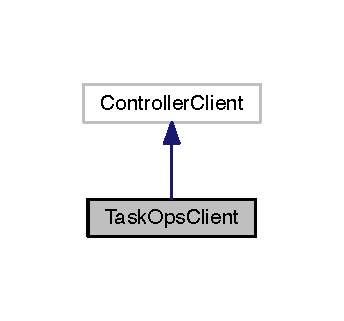
\includegraphics[width=165pt]{classTaskOpsClient__inherit__graph}
\end{center}
\end{figure}


Collaboration diagram for Task\+Ops\+Client\+:\nopagebreak
\begin{figure}[H]
\begin{center}
\leavevmode
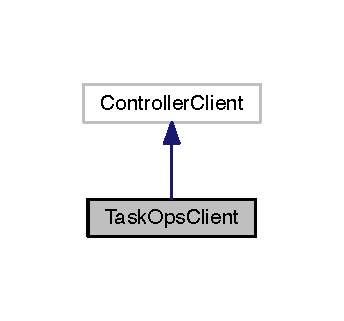
\includegraphics[width=165pt]{classTaskOpsClient__coll__graph}
\end{center}
\end{figure}
\subsection*{Public Member Functions}
\begin{DoxyCompactItemize}
\item 
\hyperlink{classTaskOpsClient_a6d3842de3255a78526ced7953428452c}{Task\+Ops\+Client} (std\+::shared\+\_\+ptr$<$ ocra\+::\+Model $>$ model\+Ptr, const int loop\+Period)
\item 
virtual \hyperlink{classTaskOpsClient_a80a5c71dd04ab7a07d4ffb8116244cdd}{$\sim$\+Task\+Ops\+Client} ()
\end{DoxyCompactItemize}
\subsection*{Protected Member Functions}
\begin{DoxyCompactItemize}
\item 
virtual bool \hyperlink{classTaskOpsClient_a6f5e4c20c1d5f5df28dcc58e3cb4adb0}{initialize} ()
\item 
virtual void \hyperlink{classTaskOpsClient_af54d37bc4a2631c5c47e23d8156f6e95}{release} ()
\item 
virtual void \hyperlink{classTaskOpsClient_a7e7dfab7af0404f0b008da2844ab573e}{loop} ()
\end{DoxyCompactItemize}
\subsection*{Private Attributes}
\begin{DoxyCompactItemize}
\item 
\hyperlink{TaskOpsClient_8h_a0140057ae3fbe1db5f5c418dfc67d9db}{T\+H\+I\+N\+G\+S\+\_\+\+T\+O\+\_\+\+DO} \hyperlink{classTaskOpsClient_a3409c4ef6b396943397b5bd9237f0a40}{thing\+To\+Do}
\end{DoxyCompactItemize}


\subsection{Constructor \& Destructor Documentation}
\hypertarget{classTaskOpsClient_a6d3842de3255a78526ced7953428452c}{}\label{classTaskOpsClient_a6d3842de3255a78526ced7953428452c} 
\index{Task\+Ops\+Client@{Task\+Ops\+Client}!Task\+Ops\+Client@{Task\+Ops\+Client}}
\index{Task\+Ops\+Client@{Task\+Ops\+Client}!Task\+Ops\+Client@{Task\+Ops\+Client}}
\subsubsection{\texorpdfstring{Task\+Ops\+Client()}{TaskOpsClient()}}
{\footnotesize\ttfamily Task\+Ops\+Client\+::\+Task\+Ops\+Client (\begin{DoxyParamCaption}\item[{std\+::shared\+\_\+ptr$<$ ocra\+::\+Model $>$}]{model\+Ptr,  }\item[{const int}]{loop\+Period }\end{DoxyParamCaption})}

\hypertarget{classTaskOpsClient_a80a5c71dd04ab7a07d4ffb8116244cdd}{}\label{classTaskOpsClient_a80a5c71dd04ab7a07d4ffb8116244cdd} 
\index{Task\+Ops\+Client@{Task\+Ops\+Client}!````~Task\+Ops\+Client@{$\sim$\+Task\+Ops\+Client}}
\index{````~Task\+Ops\+Client@{$\sim$\+Task\+Ops\+Client}!Task\+Ops\+Client@{Task\+Ops\+Client}}
\subsubsection{\texorpdfstring{$\sim$\+Task\+Ops\+Client()}{~TaskOpsClient()}}
{\footnotesize\ttfamily Task\+Ops\+Client\+::$\sim$\+Task\+Ops\+Client (\begin{DoxyParamCaption}{ }\end{DoxyParamCaption})\hspace{0.3cm}{\ttfamily [virtual]}}



\subsection{Member Function Documentation}
\hypertarget{classTaskOpsClient_a6f5e4c20c1d5f5df28dcc58e3cb4adb0}{}\label{classTaskOpsClient_a6f5e4c20c1d5f5df28dcc58e3cb4adb0} 
\index{Task\+Ops\+Client@{Task\+Ops\+Client}!initialize@{initialize}}
\index{initialize@{initialize}!Task\+Ops\+Client@{Task\+Ops\+Client}}
\subsubsection{\texorpdfstring{initialize()}{initialize()}}
{\footnotesize\ttfamily bool Task\+Ops\+Client\+::initialize (\begin{DoxyParamCaption}{ }\end{DoxyParamCaption})\hspace{0.3cm}{\ttfamily [protected]}, {\ttfamily [virtual]}}

\hypertarget{classTaskOpsClient_a7e7dfab7af0404f0b008da2844ab573e}{}\label{classTaskOpsClient_a7e7dfab7af0404f0b008da2844ab573e} 
\index{Task\+Ops\+Client@{Task\+Ops\+Client}!loop@{loop}}
\index{loop@{loop}!Task\+Ops\+Client@{Task\+Ops\+Client}}
\subsubsection{\texorpdfstring{loop()}{loop()}}
{\footnotesize\ttfamily void Task\+Ops\+Client\+::loop (\begin{DoxyParamCaption}{ }\end{DoxyParamCaption})\hspace{0.3cm}{\ttfamily [protected]}, {\ttfamily [virtual]}}

\hypertarget{classTaskOpsClient_af54d37bc4a2631c5c47e23d8156f6e95}{}\label{classTaskOpsClient_af54d37bc4a2631c5c47e23d8156f6e95} 
\index{Task\+Ops\+Client@{Task\+Ops\+Client}!release@{release}}
\index{release@{release}!Task\+Ops\+Client@{Task\+Ops\+Client}}
\subsubsection{\texorpdfstring{release()}{release()}}
{\footnotesize\ttfamily void Task\+Ops\+Client\+::release (\begin{DoxyParamCaption}{ }\end{DoxyParamCaption})\hspace{0.3cm}{\ttfamily [protected]}, {\ttfamily [virtual]}}



\subsection{Member Data Documentation}
\hypertarget{classTaskOpsClient_a3409c4ef6b396943397b5bd9237f0a40}{}\label{classTaskOpsClient_a3409c4ef6b396943397b5bd9237f0a40} 
\index{Task\+Ops\+Client@{Task\+Ops\+Client}!thing\+To\+Do@{thing\+To\+Do}}
\index{thing\+To\+Do@{thing\+To\+Do}!Task\+Ops\+Client@{Task\+Ops\+Client}}
\subsubsection{\texorpdfstring{thing\+To\+Do}{thingToDo}}
{\footnotesize\ttfamily \hyperlink{TaskOpsClient_8h_a0140057ae3fbe1db5f5c418dfc67d9db}{T\+H\+I\+N\+G\+S\+\_\+\+T\+O\+\_\+\+DO} Task\+Ops\+Client\+::thing\+To\+Do\hspace{0.3cm}{\ttfamily [private]}}



The documentation for this class was generated from the following files\+:\begin{DoxyCompactItemize}
\item 
/\+Users/jorhabibeljaik/\+Code/codyco-\/superbuild/main/ocra-\/wbi-\/plugins/ocra-\/icub-\/clients/task-\/operations-\/demo/include/task-\/operations-\/demo/\hyperlink{TaskOpsClient_8h}{Task\+Ops\+Client.\+h}\item 
/\+Users/jorhabibeljaik/\+Code/codyco-\/superbuild/main/ocra-\/wbi-\/plugins/ocra-\/icub-\/clients/task-\/operations-\/demo/src/\hyperlink{TaskOpsClient_8cpp}{Task\+Ops\+Client.\+cpp}\end{DoxyCompactItemize}

\hypertarget{classThread}{}\section{Thread Class Reference}
\label{classThread}\index{Thread@{Thread}}


The meat and potatoes of the controller server.  




{\ttfamily \#include $<$Thread.\+h$>$}

Inheritance diagram for Thread\+:\begin{figure}[H]
\begin{center}
\leavevmode
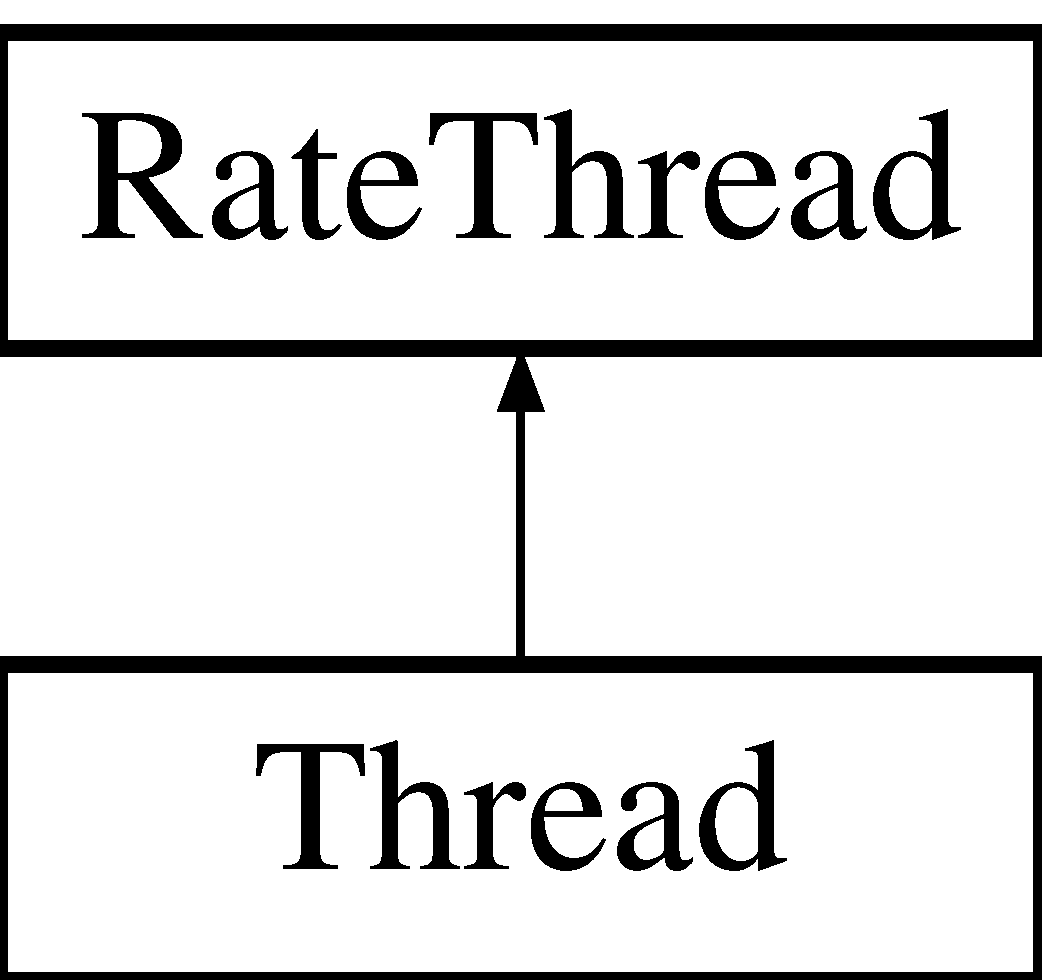
\includegraphics[height=2.000000cm]{classThread}
\end{center}
\end{figure}
\subsection*{Classes}
\begin{DoxyCompactItemize}
\item 
class \hyperlink{classThread_1_1ControllerRpcServerCallback}{Controller\+Rpc\+Server\+Callback}
\begin{DoxyCompactList}\small\item\em A callback function which binds the rpc server port opened in the contoller server module to the controller thread\textquotesingle{}s parsing function. \end{DoxyCompactList}\item 
class \hyperlink{classThread_1_1DebugRpcServerCallback}{Debug\+Rpc\+Server\+Callback}
\begin{DoxyCompactList}\small\item\em A callback function which binds the rpc server port opened in the contoller server module to the controller thread\textquotesingle{}s parsing function. \end{DoxyCompactList}\end{DoxyCompactItemize}
\subsection*{Public Member Functions}
\begin{DoxyCompactItemize}
\item 
\hyperlink{classThread_a7494a3cf676527432ee724d59ed9ee8f}{Thread} (\hyperlink{classOcraControllerOptions}{Ocra\+Controller\+Options} \&controller\+\_\+options, std\+::shared\+\_\+ptr$<$ wbi\+::whole\+Body\+Interface $>$ wbi)
\item 
virtual \hyperlink{classThread_a37d9edd3a1a776cbc27dedff949c9726}{$\sim$\+Thread} ()
\item 
bool \hyperlink{classThread_a1e840470cd71d7bfb2430d24169e3dce}{thread\+Init} ()
\item 
void \hyperlink{classThread_ad9373d8d725c46717dfce3130018fe3a}{run} ()
\item 
void \hyperlink{classThread_aa2856c7d45670f45d66bcb319255defe}{thread\+Release} ()
\end{DoxyCompactItemize}
\subsection*{Private Member Functions}
\begin{DoxyCompactItemize}
\item 
void \hyperlink{classThread_ae21029d250ac7c720f2411eab71a9414}{parse\+Incoming\+Message} (yarp\+::os\+::\+Bottle \&input, yarp\+::os\+::\+Bottle \&reply)
\item 
void \hyperlink{classThread_a6ce5ef9684cb2793be85e7402ad672f0}{parse\+Debug\+Message} (yarp\+::os\+::\+Bottle \&input, yarp\+::os\+::\+Bottle \&reply)
\item 
void \hyperlink{classThread_a9af0e98aa9b1de2f5c7bfa2f6e5001a2}{write\+Debug\+Data} ()
\end{DoxyCompactItemize}
\subsection*{Private Attributes}
\begin{DoxyCompactItemize}
\item 
ocra\+::\+Model\+::\+Ptr \hyperlink{classThread_a1dcef9aedc1a707e6f04d5fb6e4a0b13}{model}
\item 
std\+::shared\+\_\+ptr$<$ \hyperlink{classIcubControllerServer}{Icub\+Controller\+Server} $>$ \hyperlink{classThread_ace1179249de64e545f43dc48529fbbb6}{ctrl\+Server}
\item 
Eigen\+::\+Array\+Xd \hyperlink{classThread_a414015415c64371877d6028417c4f9e2}{min\+Torques}
\item 
Eigen\+::\+Array\+Xd \hyperlink{classThread_af28a4fcbbcbf77c42237c0be75a25a54}{max\+Torques}
\item 
\hyperlink{classOcraControllerOptions}{Ocra\+Controller\+Options} \hyperlink{classThread_af96a166364f0c6a680115600b3bd232e}{ctrl\+Options}
\item 
std\+::shared\+\_\+ptr$<$ wbi\+::whole\+Body\+Interface $>$ \hyperlink{classThread_aa3f4bbc2dca15c247a13de1bdbc4f7a3}{yarp\+Wbi}
\item 
Eigen\+::\+Vector\+Xd \hyperlink{classThread_a3238993799b36af06f3858a3f65dcf1e}{torques}
\item 
Eigen\+::\+Vector\+Xd \hyperlink{classThread_aa59863bb50c8aa88fe5872e75be44cb7}{initial\+Posture}
\item 
\hyperlink{namespaceocra__icub_afbd2db66b68005fb7cfac19210caf83f}{ocra\+\_\+icub\+::\+O\+C\+R\+A\+\_\+\+I\+C\+U\+B\+\_\+\+M\+E\+S\+S\+A\+GE} \hyperlink{classThread_a913cf23e86cdaefd036b782f7417254d}{controller\+Status}
\item 
Controller\+Rpc\+Server\+Callback\+::shared\+\_\+ptr \hyperlink{classThread_a602de8d12886c9c57b5420c83804a38b}{rpc\+Server\+Callback}
\item 
yarp\+::os\+::\+Rpc\+Server \hyperlink{classThread_adbec1b4f2c8fc40641df6f118e93fd25}{rpc\+Server\+Port}
\item 
int \hyperlink{classThread_aedf960b8e991868561f35193702245b0}{debug\+Joint\+Index}
\item 
yarp\+::os\+::\+Rpc\+Server \hyperlink{classThread_aa6b8f3712e7776d560b0a535eff73c34}{debug\+Rpc\+Port}
\item 
yarp\+::os\+::\+Port \hyperlink{classThread_a3780b51f82c50fd2738afbd0ae9b9526}{debug\+Ref\+Out\+Port}
\item 
yarp\+::os\+::\+Port \hyperlink{classThread_a9bd7f6aebc0be4709f32f95aa32f1add}{debug\+Real\+Out\+Port}
\item 
Debug\+Rpc\+Server\+Callback\+::shared\+\_\+ptr \hyperlink{classThread_a42833af67d5280e6946a31a03737e017}{debug\+Rpc\+Callback}
\item 
Eigen\+::\+Vector\+Xd \hyperlink{classThread_aa9cbe8744e51571a17fa726d8d16a0c6}{measured\+Torques}
\item 
bool \hyperlink{classThread_aba345996b91a57d9e1f2dd15c7c75e08}{debugging\+All\+Joints}
\item 
i\+Dyn\+Tree\+::\+Simple\+Legged\+Odometry \hyperlink{classThread_a23a41c6ccd1df898084112cfd46120f3}{odometry}
\end{DoxyCompactItemize}
\subsection*{Static Private Attributes}
\begin{DoxyCompactItemize}
\item 
static const int \hyperlink{classThread_a875b3311a39e3b87dbc981f2db7b1b9d}{A\+L\+L\+\_\+\+J\+O\+I\+N\+TS} = -\/1
\item 
static const int \hyperlink{classThread_ad44e5fbda8070c252ea71823a4b9a6db}{T\+O\+R\+Q\+U\+E\+\_\+\+M\+IN} = -\/24
\item 
static const int \hyperlink{classThread_a5e864394c4bd0fbdf3cba7f6f825e17d}{T\+O\+R\+Q\+U\+E\+\_\+\+M\+AX} = 24
\end{DoxyCompactItemize}


\subsection{Detailed Description}
The meat and potatoes of the controller server. 

\begin{DoxyRefDesc}{Todo}
\item[\hyperlink{todo__todo000001}{Todo}]Remove task sequences. This class sets up an ocra\+::\+Model which is constructed from an Ocra\+Wbi\+Model and an ocra\+::\+Controller which can be specified as either a Wocra\+Controller, a Gocra\+Controller, or a Hocra\+Controller. The thread is looped at the period specified by the user (defaults to 10ms) and on each loop the Model is updated and the control torques are recalculated. {\itshape At the writing of this comment, task sequences are still in use and they too are initialized and updated here. They will be removed eventually.} \end{DoxyRefDesc}


\subsection{Constructor \& Destructor Documentation}
\hypertarget{classThread_a7494a3cf676527432ee724d59ed9ee8f}{}\label{classThread_a7494a3cf676527432ee724d59ed9ee8f} 
\index{Thread@{Thread}!Thread@{Thread}}
\index{Thread@{Thread}!Thread@{Thread}}
\subsubsection{\texorpdfstring{Thread()}{Thread()}}
{\footnotesize\ttfamily Thread\+::\+Thread (\begin{DoxyParamCaption}\item[{\hyperlink{classOcraControllerOptions}{Ocra\+Controller\+Options} \&}]{controller\+\_\+options,  }\item[{std\+::shared\+\_\+ptr$<$ wbi\+::whole\+Body\+Interface $>$}]{wbi }\end{DoxyParamCaption})}

Constructor 
\begin{DoxyParams}{Parameters}
{\em controller\+\_\+options} & The various arguments and options used to define what type of controller and tasks to use. See \hyperlink{classOcraControllerOptions}{Ocra\+Controller\+Options}. \\
\hline
{\em wbi} & A shared pointer to a whole\+Body\+Interface object. \\
\hline
\end{DoxyParams}
\hypertarget{classThread_a37d9edd3a1a776cbc27dedff949c9726}{}\label{classThread_a37d9edd3a1a776cbc27dedff949c9726} 
\index{Thread@{Thread}!````~Thread@{$\sim$\+Thread}}
\index{````~Thread@{$\sim$\+Thread}!Thread@{Thread}}
\subsubsection{\texorpdfstring{$\sim$\+Thread()}{~Thread()}}
{\footnotesize\ttfamily Thread\+::$\sim$\+Thread (\begin{DoxyParamCaption}{ }\end{DoxyParamCaption})\hspace{0.3cm}{\ttfamily [virtual]}}



\subsection{Member Function Documentation}
\hypertarget{classThread_a6ce5ef9684cb2793be85e7402ad672f0}{}\label{classThread_a6ce5ef9684cb2793be85e7402ad672f0} 
\index{Thread@{Thread}!parse\+Debug\+Message@{parse\+Debug\+Message}}
\index{parse\+Debug\+Message@{parse\+Debug\+Message}!Thread@{Thread}}
\subsubsection{\texorpdfstring{parse\+Debug\+Message()}{parseDebugMessage()}}
{\footnotesize\ttfamily void Thread\+::parse\+Debug\+Message (\begin{DoxyParamCaption}\item[{yarp\+::os\+::\+Bottle \&}]{input,  }\item[{yarp\+::os\+::\+Bottle \&}]{reply }\end{DoxyParamCaption})\hspace{0.3cm}{\ttfamily [private]}}

\hypertarget{classThread_ae21029d250ac7c720f2411eab71a9414}{}\label{classThread_ae21029d250ac7c720f2411eab71a9414} 
\index{Thread@{Thread}!parse\+Incoming\+Message@{parse\+Incoming\+Message}}
\index{parse\+Incoming\+Message@{parse\+Incoming\+Message}!Thread@{Thread}}
\subsubsection{\texorpdfstring{parse\+Incoming\+Message()}{parseIncomingMessage()}}
{\footnotesize\ttfamily void Thread\+::parse\+Incoming\+Message (\begin{DoxyParamCaption}\item[{yarp\+::os\+::\+Bottle \&}]{input,  }\item[{yarp\+::os\+::\+Bottle \&}]{reply }\end{DoxyParamCaption})\hspace{0.3cm}{\ttfamily [private]}}

\hypertarget{classThread_ad9373d8d725c46717dfce3130018fe3a}{}\label{classThread_ad9373d8d725c46717dfce3130018fe3a} 
\index{Thread@{Thread}!run@{run}}
\index{run@{run}!Thread@{Thread}}
\subsubsection{\texorpdfstring{run()}{run()}}
{\footnotesize\ttfamily void Thread\+::run (\begin{DoxyParamCaption}{ }\end{DoxyParamCaption})}

\hypertarget{classThread_a1e840470cd71d7bfb2430d24169e3dce}{}\label{classThread_a1e840470cd71d7bfb2430d24169e3dce} 
\index{Thread@{Thread}!thread\+Init@{thread\+Init}}
\index{thread\+Init@{thread\+Init}!Thread@{Thread}}
\subsubsection{\texorpdfstring{thread\+Init()}{threadInit()}}
{\footnotesize\ttfamily bool Thread\+::thread\+Init (\begin{DoxyParamCaption}{ }\end{DoxyParamCaption})}

\hypertarget{classThread_aa2856c7d45670f45d66bcb319255defe}{}\label{classThread_aa2856c7d45670f45d66bcb319255defe} 
\index{Thread@{Thread}!thread\+Release@{thread\+Release}}
\index{thread\+Release@{thread\+Release}!Thread@{Thread}}
\subsubsection{\texorpdfstring{thread\+Release()}{threadRelease()}}
{\footnotesize\ttfamily void Thread\+::thread\+Release (\begin{DoxyParamCaption}{ }\end{DoxyParamCaption})}

\hypertarget{classThread_a9af0e98aa9b1de2f5c7bfa2f6e5001a2}{}\label{classThread_a9af0e98aa9b1de2f5c7bfa2f6e5001a2} 
\index{Thread@{Thread}!write\+Debug\+Data@{write\+Debug\+Data}}
\index{write\+Debug\+Data@{write\+Debug\+Data}!Thread@{Thread}}
\subsubsection{\texorpdfstring{write\+Debug\+Data()}{writeDebugData()}}
{\footnotesize\ttfamily void Thread\+::write\+Debug\+Data (\begin{DoxyParamCaption}{ }\end{DoxyParamCaption})\hspace{0.3cm}{\ttfamily [private]}}



\subsection{Member Data Documentation}
\hypertarget{classThread_a875b3311a39e3b87dbc981f2db7b1b9d}{}\label{classThread_a875b3311a39e3b87dbc981f2db7b1b9d} 
\index{Thread@{Thread}!A\+L\+L\+\_\+\+J\+O\+I\+N\+TS@{A\+L\+L\+\_\+\+J\+O\+I\+N\+TS}}
\index{A\+L\+L\+\_\+\+J\+O\+I\+N\+TS@{A\+L\+L\+\_\+\+J\+O\+I\+N\+TS}!Thread@{Thread}}
\subsubsection{\texorpdfstring{A\+L\+L\+\_\+\+J\+O\+I\+N\+TS}{ALL\_JOINTS}}
{\footnotesize\ttfamily const int Thread\+::\+A\+L\+L\+\_\+\+J\+O\+I\+N\+TS = -\/1\hspace{0.3cm}{\ttfamily [static]}, {\ttfamily [private]}}

Maximum possible actuator torques \hypertarget{classThread_a913cf23e86cdaefd036b782f7417254d}{}\label{classThread_a913cf23e86cdaefd036b782f7417254d} 
\index{Thread@{Thread}!controller\+Status@{controller\+Status}}
\index{controller\+Status@{controller\+Status}!Thread@{Thread}}
\subsubsection{\texorpdfstring{controller\+Status}{controllerStatus}}
{\footnotesize\ttfamily \hyperlink{namespaceocra__icub_afbd2db66b68005fb7cfac19210caf83f}{ocra\+\_\+icub\+::\+O\+C\+R\+A\+\_\+\+I\+C\+U\+B\+\_\+\+M\+E\+S\+S\+A\+GE} Thread\+::controller\+Status\hspace{0.3cm}{\ttfamily [private]}}

\hypertarget{classThread_af96a166364f0c6a680115600b3bd232e}{}\label{classThread_af96a166364f0c6a680115600b3bd232e} 
\index{Thread@{Thread}!ctrl\+Options@{ctrl\+Options}}
\index{ctrl\+Options@{ctrl\+Options}!Thread@{Thread}}
\subsubsection{\texorpdfstring{ctrl\+Options}{ctrlOptions}}
{\footnotesize\ttfamily \hyperlink{classOcraControllerOptions}{Ocra\+Controller\+Options} Thread\+::ctrl\+Options\hspace{0.3cm}{\ttfamily [private]}}

The controller options. \hypertarget{classThread_ace1179249de64e545f43dc48529fbbb6}{}\label{classThread_ace1179249de64e545f43dc48529fbbb6} 
\index{Thread@{Thread}!ctrl\+Server@{ctrl\+Server}}
\index{ctrl\+Server@{ctrl\+Server}!Thread@{Thread}}
\subsubsection{\texorpdfstring{ctrl\+Server}{ctrlServer}}
{\footnotesize\ttfamily std\+::shared\+\_\+ptr$<$\hyperlink{classIcubControllerServer}{Icub\+Controller\+Server}$>$ Thread\+::ctrl\+Server\hspace{0.3cm}{\ttfamily [private]}}

\hypertarget{classThread_aba345996b91a57d9e1f2dd15c7c75e08}{}\label{classThread_aba345996b91a57d9e1f2dd15c7c75e08} 
\index{Thread@{Thread}!debugging\+All\+Joints@{debugging\+All\+Joints}}
\index{debugging\+All\+Joints@{debugging\+All\+Joints}!Thread@{Thread}}
\subsubsection{\texorpdfstring{debugging\+All\+Joints}{debuggingAllJoints}}
{\footnotesize\ttfamily bool Thread\+::debugging\+All\+Joints\hspace{0.3cm}{\ttfamily [private]}}

\hypertarget{classThread_aedf960b8e991868561f35193702245b0}{}\label{classThread_aedf960b8e991868561f35193702245b0} 
\index{Thread@{Thread}!debug\+Joint\+Index@{debug\+Joint\+Index}}
\index{debug\+Joint\+Index@{debug\+Joint\+Index}!Thread@{Thread}}
\subsubsection{\texorpdfstring{debug\+Joint\+Index}{debugJointIndex}}
{\footnotesize\ttfamily int Thread\+::debug\+Joint\+Index\hspace{0.3cm}{\ttfamily [private]}}

\hypertarget{classThread_a9bd7f6aebc0be4709f32f95aa32f1add}{}\label{classThread_a9bd7f6aebc0be4709f32f95aa32f1add} 
\index{Thread@{Thread}!debug\+Real\+Out\+Port@{debug\+Real\+Out\+Port}}
\index{debug\+Real\+Out\+Port@{debug\+Real\+Out\+Port}!Thread@{Thread}}
\subsubsection{\texorpdfstring{debug\+Real\+Out\+Port}{debugRealOutPort}}
{\footnotesize\ttfamily yarp\+::os\+::\+Port Thread\+::debug\+Real\+Out\+Port\hspace{0.3cm}{\ttfamily [private]}}

\hypertarget{classThread_a3780b51f82c50fd2738afbd0ae9b9526}{}\label{classThread_a3780b51f82c50fd2738afbd0ae9b9526} 
\index{Thread@{Thread}!debug\+Ref\+Out\+Port@{debug\+Ref\+Out\+Port}}
\index{debug\+Ref\+Out\+Port@{debug\+Ref\+Out\+Port}!Thread@{Thread}}
\subsubsection{\texorpdfstring{debug\+Ref\+Out\+Port}{debugRefOutPort}}
{\footnotesize\ttfamily yarp\+::os\+::\+Port Thread\+::debug\+Ref\+Out\+Port\hspace{0.3cm}{\ttfamily [private]}}

\hypertarget{classThread_a42833af67d5280e6946a31a03737e017}{}\label{classThread_a42833af67d5280e6946a31a03737e017} 
\index{Thread@{Thread}!debug\+Rpc\+Callback@{debug\+Rpc\+Callback}}
\index{debug\+Rpc\+Callback@{debug\+Rpc\+Callback}!Thread@{Thread}}
\subsubsection{\texorpdfstring{debug\+Rpc\+Callback}{debugRpcCallback}}
{\footnotesize\ttfamily Debug\+Rpc\+Server\+Callback\+::shared\+\_\+ptr Thread\+::debug\+Rpc\+Callback\hspace{0.3cm}{\ttfamily [private]}}

Rpc server port callback function. \hypertarget{classThread_aa6b8f3712e7776d560b0a535eff73c34}{}\label{classThread_aa6b8f3712e7776d560b0a535eff73c34} 
\index{Thread@{Thread}!debug\+Rpc\+Port@{debug\+Rpc\+Port}}
\index{debug\+Rpc\+Port@{debug\+Rpc\+Port}!Thread@{Thread}}
\subsubsection{\texorpdfstring{debug\+Rpc\+Port}{debugRpcPort}}
{\footnotesize\ttfamily yarp\+::os\+::\+Rpc\+Server Thread\+::debug\+Rpc\+Port\hspace{0.3cm}{\ttfamily [private]}}

\hypertarget{classThread_aa59863bb50c8aa88fe5872e75be44cb7}{}\label{classThread_aa59863bb50c8aa88fe5872e75be44cb7} 
\index{Thread@{Thread}!initial\+Posture@{initial\+Posture}}
\index{initial\+Posture@{initial\+Posture}!Thread@{Thread}}
\subsubsection{\texorpdfstring{initial\+Posture}{initialPosture}}
{\footnotesize\ttfamily Eigen\+::\+Vector\+Xd Thread\+::initial\+Posture\hspace{0.3cm}{\ttfamily [private]}}

The torques calculated at each \hyperlink{classThread_ad9373d8d725c46717dfce3130018fe3a}{run()} loop. \hypertarget{classThread_af28a4fcbbcbf77c42237c0be75a25a54}{}\label{classThread_af28a4fcbbcbf77c42237c0be75a25a54} 
\index{Thread@{Thread}!max\+Torques@{max\+Torques}}
\index{max\+Torques@{max\+Torques}!Thread@{Thread}}
\subsubsection{\texorpdfstring{max\+Torques}{maxTorques}}
{\footnotesize\ttfamily Eigen\+::\+Array\+Xd Thread\+::max\+Torques\hspace{0.3cm}{\ttfamily [private]}}

An eigen array filled with the max torques. \hypertarget{classThread_aa9cbe8744e51571a17fa726d8d16a0c6}{}\label{classThread_aa9cbe8744e51571a17fa726d8d16a0c6} 
\index{Thread@{Thread}!measured\+Torques@{measured\+Torques}}
\index{measured\+Torques@{measured\+Torques}!Thread@{Thread}}
\subsubsection{\texorpdfstring{measured\+Torques}{measuredTorques}}
{\footnotesize\ttfamily Eigen\+::\+Vector\+Xd Thread\+::measured\+Torques\hspace{0.3cm}{\ttfamily [private]}}

\hypertarget{classThread_a414015415c64371877d6028417c4f9e2}{}\label{classThread_a414015415c64371877d6028417c4f9e2} 
\index{Thread@{Thread}!min\+Torques@{min\+Torques}}
\index{min\+Torques@{min\+Torques}!Thread@{Thread}}
\subsubsection{\texorpdfstring{min\+Torques}{minTorques}}
{\footnotesize\ttfamily Eigen\+::\+Array\+Xd Thread\+::min\+Torques\hspace{0.3cm}{\ttfamily [private]}}

An eigen array filled with the min torques. \hypertarget{classThread_a1dcef9aedc1a707e6f04d5fb6e4a0b13}{}\label{classThread_a1dcef9aedc1a707e6f04d5fb6e4a0b13} 
\index{Thread@{Thread}!model@{model}}
\index{model@{model}!Thread@{Thread}}
\subsubsection{\texorpdfstring{model}{model}}
{\footnotesize\ttfamily ocra\+::\+Model\+::\+Ptr Thread\+::model\hspace{0.3cm}{\ttfamily [private]}}

\hypertarget{classThread_a23a41c6ccd1df898084112cfd46120f3}{}\label{classThread_a23a41c6ccd1df898084112cfd46120f3} 
\index{Thread@{Thread}!odometry@{odometry}}
\index{odometry@{odometry}!Thread@{Thread}}
\subsubsection{\texorpdfstring{odometry}{odometry}}
{\footnotesize\ttfamily i\+Dyn\+Tree\+::\+Simple\+Legged\+Odometry Thread\+::odometry\hspace{0.3cm}{\ttfamily [private]}}

Odometry object \hypertarget{classThread_a602de8d12886c9c57b5420c83804a38b}{}\label{classThread_a602de8d12886c9c57b5420c83804a38b} 
\index{Thread@{Thread}!rpc\+Server\+Callback@{rpc\+Server\+Callback}}
\index{rpc\+Server\+Callback@{rpc\+Server\+Callback}!Thread@{Thread}}
\subsubsection{\texorpdfstring{rpc\+Server\+Callback}{rpcServerCallback}}
{\footnotesize\ttfamily Controller\+Rpc\+Server\+Callback\+::shared\+\_\+ptr Thread\+::rpc\+Server\+Callback\hspace{0.3cm}{\ttfamily [private]}}

Rpc server port callback function. \hypertarget{classThread_adbec1b4f2c8fc40641df6f118e93fd25}{}\label{classThread_adbec1b4f2c8fc40641df6f118e93fd25} 
\index{Thread@{Thread}!rpc\+Server\+Port@{rpc\+Server\+Port}}
\index{rpc\+Server\+Port@{rpc\+Server\+Port}!Thread@{Thread}}
\subsubsection{\texorpdfstring{rpc\+Server\+Port}{rpcServerPort}}
{\footnotesize\ttfamily yarp\+::os\+::\+Rpc\+Server Thread\+::rpc\+Server\+Port\hspace{0.3cm}{\ttfamily [private]}}

Rpc server port. \hypertarget{classThread_a5e864394c4bd0fbdf3cba7f6f825e17d}{}\label{classThread_a5e864394c4bd0fbdf3cba7f6f825e17d} 
\index{Thread@{Thread}!T\+O\+R\+Q\+U\+E\+\_\+\+M\+AX@{T\+O\+R\+Q\+U\+E\+\_\+\+M\+AX}}
\index{T\+O\+R\+Q\+U\+E\+\_\+\+M\+AX@{T\+O\+R\+Q\+U\+E\+\_\+\+M\+AX}!Thread@{Thread}}
\subsubsection{\texorpdfstring{T\+O\+R\+Q\+U\+E\+\_\+\+M\+AX}{TORQUE\_MAX}}
{\footnotesize\ttfamily const int Thread\+::\+T\+O\+R\+Q\+U\+E\+\_\+\+M\+AX = 24\hspace{0.3cm}{\ttfamily [static]}, {\ttfamily [private]}}

Maximum possible actuator torques \hypertarget{classThread_ad44e5fbda8070c252ea71823a4b9a6db}{}\label{classThread_ad44e5fbda8070c252ea71823a4b9a6db} 
\index{Thread@{Thread}!T\+O\+R\+Q\+U\+E\+\_\+\+M\+IN@{T\+O\+R\+Q\+U\+E\+\_\+\+M\+IN}}
\index{T\+O\+R\+Q\+U\+E\+\_\+\+M\+IN@{T\+O\+R\+Q\+U\+E\+\_\+\+M\+IN}!Thread@{Thread}}
\subsubsection{\texorpdfstring{T\+O\+R\+Q\+U\+E\+\_\+\+M\+IN}{TORQUE\_MIN}}
{\footnotesize\ttfamily const int Thread\+::\+T\+O\+R\+Q\+U\+E\+\_\+\+M\+IN = -\/24\hspace{0.3cm}{\ttfamily [static]}, {\ttfamily [private]}}

Minimum possible actuator torques \hypertarget{classThread_a3238993799b36af06f3858a3f65dcf1e}{}\label{classThread_a3238993799b36af06f3858a3f65dcf1e} 
\index{Thread@{Thread}!torques@{torques}}
\index{torques@{torques}!Thread@{Thread}}
\subsubsection{\texorpdfstring{torques}{torques}}
{\footnotesize\ttfamily Eigen\+::\+Vector\+Xd Thread\+::torques\hspace{0.3cm}{\ttfamily [private]}}

The torques calculated at each \hyperlink{classThread_ad9373d8d725c46717dfce3130018fe3a}{run()} loop. \hypertarget{classThread_aa3f4bbc2dca15c247a13de1bdbc4f7a3}{}\label{classThread_aa3f4bbc2dca15c247a13de1bdbc4f7a3} 
\index{Thread@{Thread}!yarp\+Wbi@{yarp\+Wbi}}
\index{yarp\+Wbi@{yarp\+Wbi}!Thread@{Thread}}
\subsubsection{\texorpdfstring{yarp\+Wbi}{yarpWbi}}
{\footnotesize\ttfamily std\+::shared\+\_\+ptr$<$wbi\+::whole\+Body\+Interface$>$ Thread\+::yarp\+Wbi\hspace{0.3cm}{\ttfamily [private]}}

The W\+BI used to talk to the robot. 

The documentation for this class was generated from the following files\+:\begin{DoxyCompactItemize}
\item 
/\+Users/jorhabibeljaik/\+Code/codyco-\/superbuild/main/ocra-\/wbi-\/plugins/ocra-\/icub-\/server/include/ocra-\/icub-\/server/\hyperlink{Thread_8h}{Thread.\+h}\item 
/\+Users/jorhabibeljaik/\+Code/codyco-\/superbuild/main/ocra-\/wbi-\/plugins/ocra-\/icub-\/server/src/\hyperlink{Thread_8cpp}{Thread.\+cpp}\end{DoxyCompactItemize}

\chapter{File Documentation}
\hypertarget{ExampleClient_8h}{}\section{/\+Users/jorhabibeljaik/\+Code/codyco-\/superbuild/main/ocra-\/wbi-\/plugins/ocra-\/icub-\/clients/example-\/client/include/example-\/client/\+Example\+Client.h File Reference}
\label{ExampleClient_8h}\index{/\+Users/jorhabibeljaik/\+Code/codyco-\/superbuild/main/ocra-\/wbi-\/plugins/ocra-\/icub-\/clients/example-\/client/include/example-\/client/\+Example\+Client.\+h@{/\+Users/jorhabibeljaik/\+Code/codyco-\/superbuild/main/ocra-\/wbi-\/plugins/ocra-\/icub-\/clients/example-\/client/include/example-\/client/\+Example\+Client.\+h}}
{\ttfamily \#include $<$ocra-\/icub/\+Icub\+Client.\+h$>$}\newline
{\ttfamily \#include $<$ocra-\/recipes/\+Trajectory\+Thread.\+h$>$}\newline
{\ttfamily \#include $<$ocra-\/recipes/\+Controller\+Client.\+h$>$}\newline
\subsection*{Classes}
\begin{DoxyCompactItemize}
\item 
class \hyperlink{classExampleClient}{Example\+Client}
\end{DoxyCompactItemize}

\hypertarget{example-client_8cpp}{}\section{/\+Users/jorhabibeljaik/\+Code/codyco-\/superbuild/main/ocra-\/wbi-\/plugins/ocra-\/icub-\/clients/example-\/client/src/example-\/client.cpp File Reference}
\label{example-client_8cpp}\index{/\+Users/jorhabibeljaik/\+Code/codyco-\/superbuild/main/ocra-\/wbi-\/plugins/ocra-\/icub-\/clients/example-\/client/src/example-\/client.\+cpp@{/\+Users/jorhabibeljaik/\+Code/codyco-\/superbuild/main/ocra-\/wbi-\/plugins/ocra-\/icub-\/clients/example-\/client/src/example-\/client.\+cpp}}
{\ttfamily \#include $<$yarp/os/\+Resource\+Finder.\+h$>$}\newline
{\ttfamily \#include $<$yarp/os/\+Network.\+h$>$}\newline
{\ttfamily \#include $<$yarp/os/\+Log.\+h$>$}\newline
{\ttfamily \#include $<$yarp/os/\+Log\+Stream.\+h$>$}\newline
{\ttfamily \#include $<$yarp/os/\+Time.\+h$>$}\newline
{\ttfamily \#include \char`\"{}example-\/client/\+Example\+Client.\+h\char`\"{}}\newline
{\ttfamily \#include $<$ocra-\/icub/\+Icub\+Client.\+h$>$}\newline
{\ttfamily \#include $<$ocra-\/recipes/\+Controller\+Client.\+h$>$}\newline
{\ttfamily \#include $<$ocra-\/recipes/\+Client\+Manager.\+h$>$}\newline
Include dependency graph for example-\/client.cpp\+:
\nopagebreak
\begin{figure}[H]
\begin{center}
\leavevmode
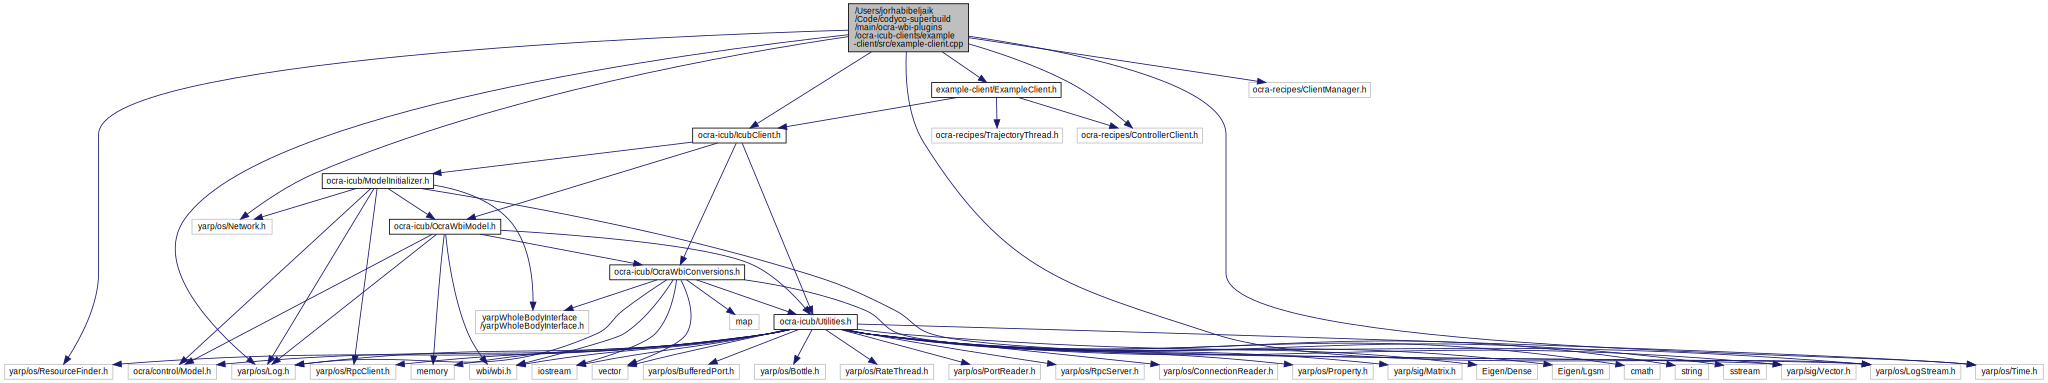
\includegraphics[width=350pt]{example-client_8cpp__incl}
\end{center}
\end{figure}
\subsection*{Functions}
\begin{DoxyCompactItemize}
\item 
int \hyperlink{example-client_8cpp_a0ddf1224851353fc92bfbff6f499fa97}{main} (int argc, char $\ast$argv\mbox{[}$\,$\mbox{]})
\end{DoxyCompactItemize}


\subsection{Detailed Description}
\begin{DoxyAuthor}{Author}
\href{http://www.ryanlober.com}{\tt Ryan Lober} 

\href{http://ahoarau.github.io}{\tt Antoine Hoarau} 
\end{DoxyAuthor}
\begin{DoxyDate}{Date}
Feb 2016 
\end{DoxyDate}
\begin{DoxyCopyright}{Copyright}
G\+NU General Public License. 
\end{DoxyCopyright}


\subsection{Function Documentation}
\hypertarget{example-client_8cpp_a0ddf1224851353fc92bfbff6f499fa97}{}\label{example-client_8cpp_a0ddf1224851353fc92bfbff6f499fa97} 
\index{example-\/client.\+cpp@{example-\/client.\+cpp}!main@{main}}
\index{main@{main}!example-\/client.\+cpp@{example-\/client.\+cpp}}
\subsubsection{\texorpdfstring{main()}{main()}}
{\footnotesize\ttfamily int main (\begin{DoxyParamCaption}\item[{int}]{argc,  }\item[{char $\ast$}]{argv\mbox{[}$\,$\mbox{]} }\end{DoxyParamCaption})}


\hypertarget{ExampleClient_8cpp}{}\section{/\+Users/jorhabibeljaik/\+Code/codyco-\/superbuild/main/ocra-\/wbi-\/plugins/ocra-\/icub-\/clients/example-\/client/src/\+Example\+Client.cpp File Reference}
\label{ExampleClient_8cpp}\index{/\+Users/jorhabibeljaik/\+Code/codyco-\/superbuild/main/ocra-\/wbi-\/plugins/ocra-\/icub-\/clients/example-\/client/src/\+Example\+Client.\+cpp@{/\+Users/jorhabibeljaik/\+Code/codyco-\/superbuild/main/ocra-\/wbi-\/plugins/ocra-\/icub-\/clients/example-\/client/src/\+Example\+Client.\+cpp}}
{\ttfamily \#include \char`\"{}example-\/client/\+Example\+Client.\+h\char`\"{}}\newline
Include dependency graph for Example\+Client.\+cpp\+:
\nopagebreak
\begin{figure}[H]
\begin{center}
\leavevmode
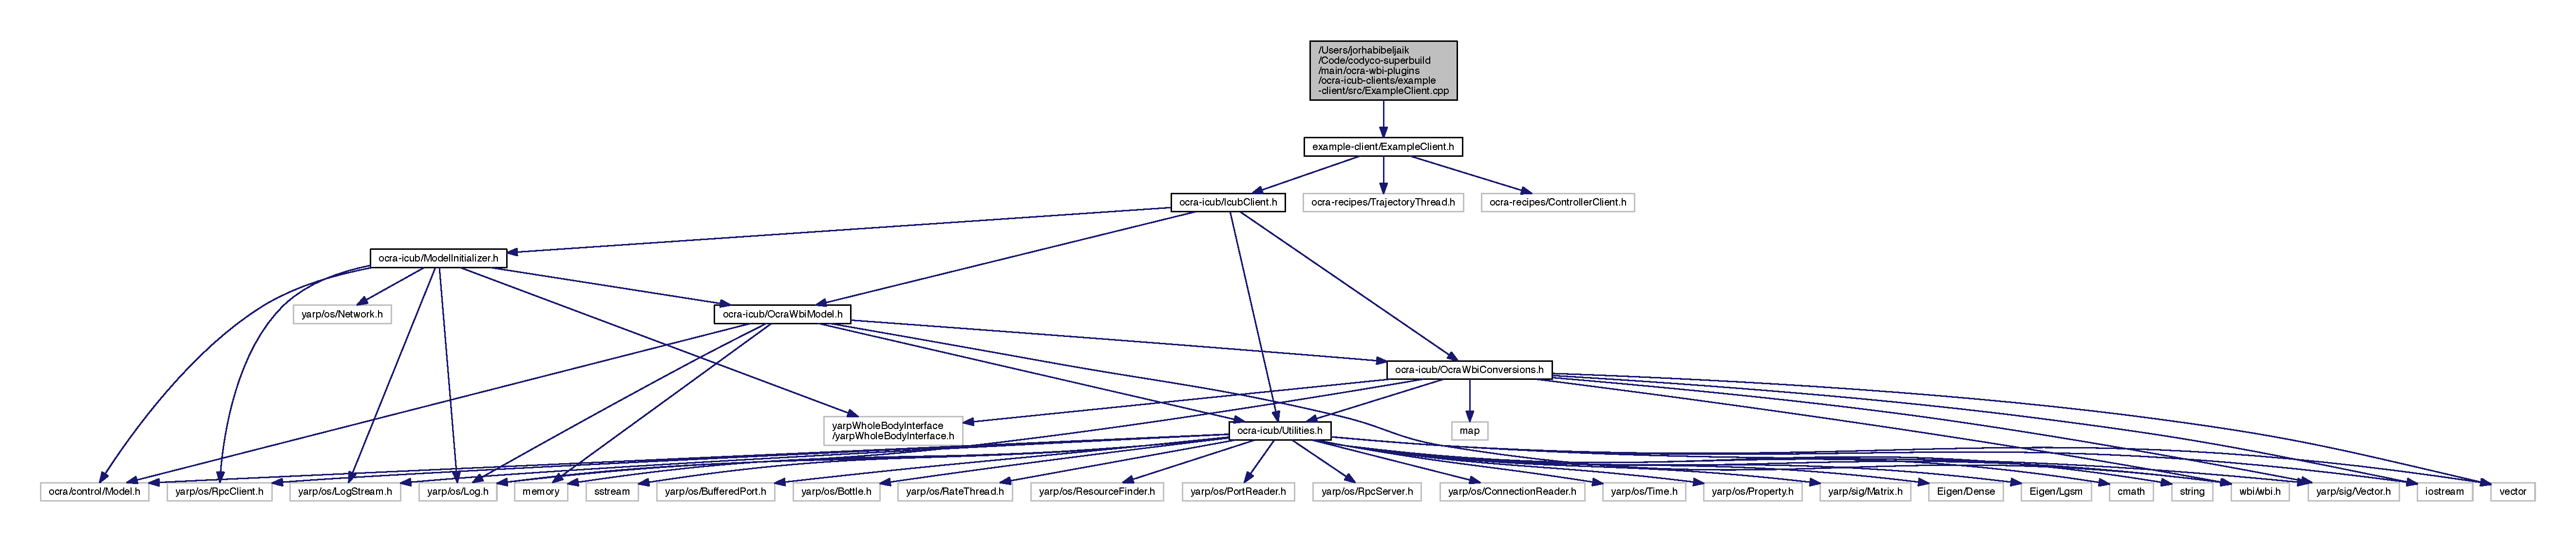
\includegraphics[width=350pt]{ExampleClient_8cpp__incl}
\end{center}
\end{figure}

\hypertarget{SteppingDemoClient_8h}{}\section{/\+Users/jorhabibeljaik/\+Code/codyco-\/superbuild/main/ocra-\/wbi-\/plugins/ocra-\/icub-\/clients/stepping-\/demo/include/stepping-\/demo/\+Stepping\+Demo\+Client.h File Reference}
\label{SteppingDemoClient_8h}\index{/\+Users/jorhabibeljaik/\+Code/codyco-\/superbuild/main/ocra-\/wbi-\/plugins/ocra-\/icub-\/clients/stepping-\/demo/include/stepping-\/demo/\+Stepping\+Demo\+Client.\+h@{/\+Users/jorhabibeljaik/\+Code/codyco-\/superbuild/main/ocra-\/wbi-\/plugins/ocra-\/icub-\/clients/stepping-\/demo/include/stepping-\/demo/\+Stepping\+Demo\+Client.\+h}}
{\ttfamily \#include $<$ocra-\/icub/\+Icub\+Client.\+h$>$}\newline
{\ttfamily \#include $<$ocra-\/recipes/\+Trajectory\+Thread.\+h$>$}\newline
{\ttfamily \#include $<$ocra-\/recipes/\+Controller\+Client.\+h$>$}\newline
{\ttfamily \#include $<$ocra/util/\+Errors\+Helper.\+h$>$}\newline
Include dependency graph for Stepping\+Demo\+Client.\+h\+:\nopagebreak
\begin{figure}[H]
\begin{center}
\leavevmode
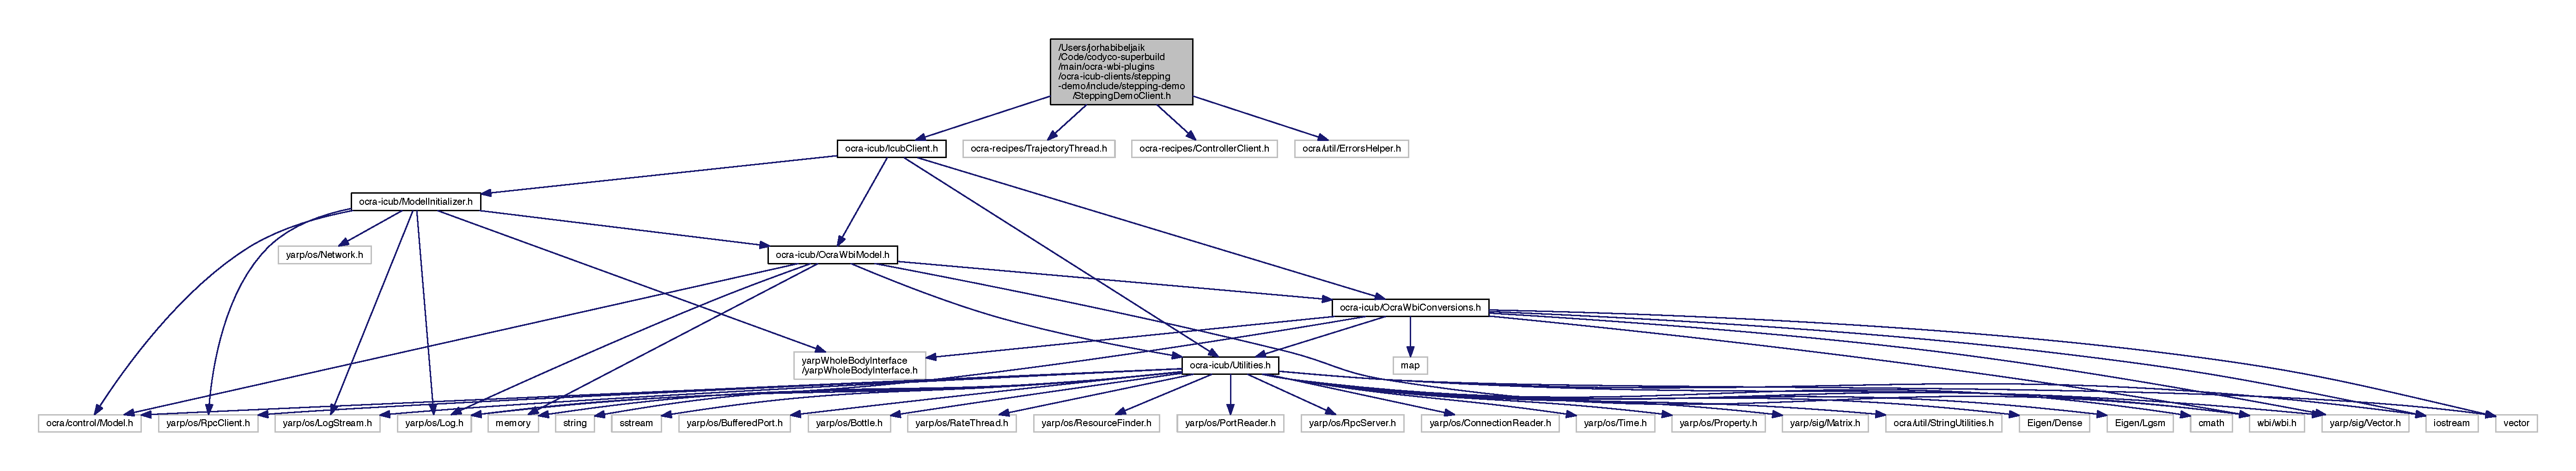
\includegraphics[width=350pt]{SteppingDemoClient_8h__incl}
\end{center}
\end{figure}
This graph shows which files directly or indirectly include this file\+:\nopagebreak
\begin{figure}[H]
\begin{center}
\leavevmode
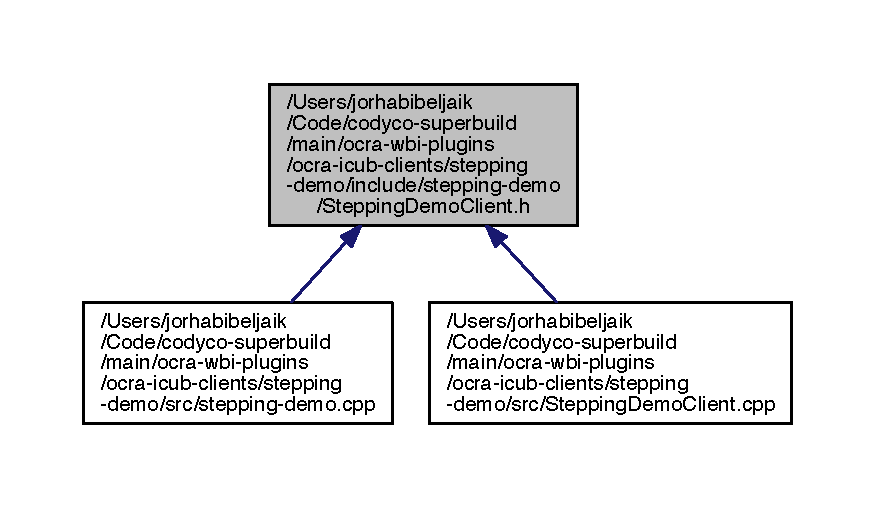
\includegraphics[width=350pt]{SteppingDemoClient_8h__dep__incl}
\end{center}
\end{figure}
\subsection*{Classes}
\begin{DoxyCompactItemize}
\item 
struct \hyperlink{structWalkingParams}{Walking\+Params}
\item 
class \hyperlink{classSteppingDemoClient}{Stepping\+Demo\+Client}
\end{DoxyCompactItemize}
\subsection*{Enumerations}
\begin{DoxyCompactItemize}
\item 
enum \hyperlink{SteppingDemoClient_8h_ac0c3848a609566394821d9826e0fdd5b}{C\+O\+M\+\_\+\+S\+U\+P\+P\+O\+R\+T\+\_\+\+P\+O\+S\+I\+T\+I\+ON} \{ \hyperlink{SteppingDemoClient_8h_ac0c3848a609566394821d9826e0fdd5ba07cd79ee915be269a43f655f31cd3ccf}{L\+E\+F\+T\+\_\+\+F\+O\+O\+T\+\_\+\+XY}, 
\hyperlink{SteppingDemoClient_8h_ac0c3848a609566394821d9826e0fdd5ba273605381ab0231d2abb4a8096faabfd}{R\+I\+G\+H\+T\+\_\+\+F\+O\+O\+T\+\_\+\+XY}, 
\hyperlink{SteppingDemoClient_8h_ac0c3848a609566394821d9826e0fdd5bad32a9ea5bb598218529abf1a5b9b50cf}{C\+E\+N\+T\+E\+R\+E\+D\+\_\+\+B\+E\+T\+W\+E\+E\+N\+\_\+\+F\+E\+E\+T\+\_\+\+XY}
 \}
\item 
enum \hyperlink{SteppingDemoClient_8h_af2a8507bf21c3ce9b0e67a23381251c6}{C\+O\+N\+T\+R\+O\+L\+\_\+\+P\+H\+A\+SE} \{ \hyperlink{SteppingDemoClient_8h_af2a8507bf21c3ce9b0e67a23381251c6afe7fc4a2f5d6778bbb96f412be37d63c}{M\+O\+V\+E\+\_\+\+T\+O\+\_\+\+L\+E\+F\+T\+\_\+\+S\+U\+P\+P\+O\+RT}, 
\hyperlink{SteppingDemoClient_8h_af2a8507bf21c3ce9b0e67a23381251c6a3b4335037acf972dd5d60348ca20d394}{M\+O\+V\+E\+\_\+\+T\+O\+\_\+\+R\+I\+G\+H\+T\+\_\+\+S\+U\+P\+P\+O\+RT}, 
\hyperlink{SteppingDemoClient_8h_af2a8507bf21c3ce9b0e67a23381251c6a362d8557e44bcc19f6b4d9096bb54401}{M\+O\+V\+E\+\_\+\+T\+O\+\_\+\+D\+O\+U\+B\+L\+E\+\_\+\+S\+U\+P\+P\+O\+RT}, 
\hyperlink{SteppingDemoClient_8h_af2a8507bf21c3ce9b0e67a23381251c6a4ff6c6ae9503ea4bca745c7d7819523e}{S\+T\+E\+P\+\_\+\+F\+O\+R\+W\+A\+RD}
 \}
\item 
enum \hyperlink{SteppingDemoClient_8h_ab0673d7f17cdd57b8fa124abb330287f}{F\+O\+O\+T\+\_\+\+C\+O\+N\+T\+A\+C\+TS} \{ \hyperlink{SteppingDemoClient_8h_ab0673d7f17cdd57b8fa124abb330287fa7760daad9db1ede8c57b06189deca9f3}{L\+E\+F\+T\+\_\+\+F\+O\+OT}, 
\hyperlink{SteppingDemoClient_8h_ab0673d7f17cdd57b8fa124abb330287face119c66af60ac0781b137aa87d7be62}{R\+I\+G\+H\+T\+\_\+\+F\+O\+OT}
 \}
\item 
enum \hyperlink{SteppingDemoClient_8h_abd6d177d63e98aa1b4ed4b8329e2a379}{M\+O\+T\+I\+O\+N\+\_\+\+T\+Y\+PE} \{ \hyperlink{SteppingDemoClient_8h_abd6d177d63e98aa1b4ed4b8329e2a379a55b57dce74f14a62104ae66e62789eb3}{L\+E\+F\+T\+\_\+\+T\+O\+\_\+\+R\+I\+G\+HT}, 
\hyperlink{SteppingDemoClient_8h_abd6d177d63e98aa1b4ed4b8329e2a379ada7017955bb1db9f0954017358028fa6}{S\+T\+A\+T\+I\+C\+\_\+\+W\+A\+L\+K\+I\+NG}
 \}
\end{DoxyCompactItemize}


\subsection{Enumeration Type Documentation}
\hypertarget{SteppingDemoClient_8h_ac0c3848a609566394821d9826e0fdd5b}{}\label{SteppingDemoClient_8h_ac0c3848a609566394821d9826e0fdd5b} 
\index{Stepping\+Demo\+Client.\+h@{Stepping\+Demo\+Client.\+h}!C\+O\+M\+\_\+\+S\+U\+P\+P\+O\+R\+T\+\_\+\+P\+O\+S\+I\+T\+I\+ON@{C\+O\+M\+\_\+\+S\+U\+P\+P\+O\+R\+T\+\_\+\+P\+O\+S\+I\+T\+I\+ON}}
\index{C\+O\+M\+\_\+\+S\+U\+P\+P\+O\+R\+T\+\_\+\+P\+O\+S\+I\+T\+I\+ON@{C\+O\+M\+\_\+\+S\+U\+P\+P\+O\+R\+T\+\_\+\+P\+O\+S\+I\+T\+I\+ON}!Stepping\+Demo\+Client.\+h@{Stepping\+Demo\+Client.\+h}}
\subsubsection{\texorpdfstring{C\+O\+M\+\_\+\+S\+U\+P\+P\+O\+R\+T\+\_\+\+P\+O\+S\+I\+T\+I\+ON}{COM\_SUPPORT\_POSITION}}
{\footnotesize\ttfamily enum \hyperlink{SteppingDemoClient_8h_ac0c3848a609566394821d9826e0fdd5b}{C\+O\+M\+\_\+\+S\+U\+P\+P\+O\+R\+T\+\_\+\+P\+O\+S\+I\+T\+I\+ON}}

\begin{DoxyEnumFields}{Enumerator}
\raisebox{\heightof{T}}[0pt][0pt]{\index{L\+E\+F\+T\+\_\+\+F\+O\+O\+T\+\_\+\+XY@{L\+E\+F\+T\+\_\+\+F\+O\+O\+T\+\_\+\+XY}!Stepping\+Demo\+Client.\+h@{Stepping\+Demo\+Client.\+h}}\index{Stepping\+Demo\+Client.\+h@{Stepping\+Demo\+Client.\+h}!L\+E\+F\+T\+\_\+\+F\+O\+O\+T\+\_\+\+XY@{L\+E\+F\+T\+\_\+\+F\+O\+O\+T\+\_\+\+XY}}}\hypertarget{SteppingDemoClient_8h_ac0c3848a609566394821d9826e0fdd5ba07cd79ee915be269a43f655f31cd3ccf}{}\label{SteppingDemoClient_8h_ac0c3848a609566394821d9826e0fdd5ba07cd79ee915be269a43f655f31cd3ccf} 
L\+E\+F\+T\+\_\+\+F\+O\+O\+T\+\_\+\+XY&\\
\hline

\raisebox{\heightof{T}}[0pt][0pt]{\index{R\+I\+G\+H\+T\+\_\+\+F\+O\+O\+T\+\_\+\+XY@{R\+I\+G\+H\+T\+\_\+\+F\+O\+O\+T\+\_\+\+XY}!Stepping\+Demo\+Client.\+h@{Stepping\+Demo\+Client.\+h}}\index{Stepping\+Demo\+Client.\+h@{Stepping\+Demo\+Client.\+h}!R\+I\+G\+H\+T\+\_\+\+F\+O\+O\+T\+\_\+\+XY@{R\+I\+G\+H\+T\+\_\+\+F\+O\+O\+T\+\_\+\+XY}}}\hypertarget{SteppingDemoClient_8h_ac0c3848a609566394821d9826e0fdd5ba273605381ab0231d2abb4a8096faabfd}{}\label{SteppingDemoClient_8h_ac0c3848a609566394821d9826e0fdd5ba273605381ab0231d2abb4a8096faabfd} 
R\+I\+G\+H\+T\+\_\+\+F\+O\+O\+T\+\_\+\+XY&\\
\hline

\raisebox{\heightof{T}}[0pt][0pt]{\index{C\+E\+N\+T\+E\+R\+E\+D\+\_\+\+B\+E\+T\+W\+E\+E\+N\+\_\+\+F\+E\+E\+T\+\_\+\+XY@{C\+E\+N\+T\+E\+R\+E\+D\+\_\+\+B\+E\+T\+W\+E\+E\+N\+\_\+\+F\+E\+E\+T\+\_\+\+XY}!Stepping\+Demo\+Client.\+h@{Stepping\+Demo\+Client.\+h}}\index{Stepping\+Demo\+Client.\+h@{Stepping\+Demo\+Client.\+h}!C\+E\+N\+T\+E\+R\+E\+D\+\_\+\+B\+E\+T\+W\+E\+E\+N\+\_\+\+F\+E\+E\+T\+\_\+\+XY@{C\+E\+N\+T\+E\+R\+E\+D\+\_\+\+B\+E\+T\+W\+E\+E\+N\+\_\+\+F\+E\+E\+T\+\_\+\+XY}}}\hypertarget{SteppingDemoClient_8h_ac0c3848a609566394821d9826e0fdd5bad32a9ea5bb598218529abf1a5b9b50cf}{}\label{SteppingDemoClient_8h_ac0c3848a609566394821d9826e0fdd5bad32a9ea5bb598218529abf1a5b9b50cf} 
C\+E\+N\+T\+E\+R\+E\+D\+\_\+\+B\+E\+T\+W\+E\+E\+N\+\_\+\+F\+E\+E\+T\+\_\+\+XY&\\
\hline

\end{DoxyEnumFields}
\hypertarget{SteppingDemoClient_8h_af2a8507bf21c3ce9b0e67a23381251c6}{}\label{SteppingDemoClient_8h_af2a8507bf21c3ce9b0e67a23381251c6} 
\index{Stepping\+Demo\+Client.\+h@{Stepping\+Demo\+Client.\+h}!C\+O\+N\+T\+R\+O\+L\+\_\+\+P\+H\+A\+SE@{C\+O\+N\+T\+R\+O\+L\+\_\+\+P\+H\+A\+SE}}
\index{C\+O\+N\+T\+R\+O\+L\+\_\+\+P\+H\+A\+SE@{C\+O\+N\+T\+R\+O\+L\+\_\+\+P\+H\+A\+SE}!Stepping\+Demo\+Client.\+h@{Stepping\+Demo\+Client.\+h}}
\subsubsection{\texorpdfstring{C\+O\+N\+T\+R\+O\+L\+\_\+\+P\+H\+A\+SE}{CONTROL\_PHASE}}
{\footnotesize\ttfamily enum \hyperlink{SteppingDemoClient_8h_af2a8507bf21c3ce9b0e67a23381251c6}{C\+O\+N\+T\+R\+O\+L\+\_\+\+P\+H\+A\+SE}}

\begin{DoxyEnumFields}{Enumerator}
\raisebox{\heightof{T}}[0pt][0pt]{\index{M\+O\+V\+E\+\_\+\+T\+O\+\_\+\+L\+E\+F\+T\+\_\+\+S\+U\+P\+P\+O\+RT@{M\+O\+V\+E\+\_\+\+T\+O\+\_\+\+L\+E\+F\+T\+\_\+\+S\+U\+P\+P\+O\+RT}!Stepping\+Demo\+Client.\+h@{Stepping\+Demo\+Client.\+h}}\index{Stepping\+Demo\+Client.\+h@{Stepping\+Demo\+Client.\+h}!M\+O\+V\+E\+\_\+\+T\+O\+\_\+\+L\+E\+F\+T\+\_\+\+S\+U\+P\+P\+O\+RT@{M\+O\+V\+E\+\_\+\+T\+O\+\_\+\+L\+E\+F\+T\+\_\+\+S\+U\+P\+P\+O\+RT}}}\hypertarget{SteppingDemoClient_8h_af2a8507bf21c3ce9b0e67a23381251c6afe7fc4a2f5d6778bbb96f412be37d63c}{}\label{SteppingDemoClient_8h_af2a8507bf21c3ce9b0e67a23381251c6afe7fc4a2f5d6778bbb96f412be37d63c} 
M\+O\+V\+E\+\_\+\+T\+O\+\_\+\+L\+E\+F\+T\+\_\+\+S\+U\+P\+P\+O\+RT&\\
\hline

\raisebox{\heightof{T}}[0pt][0pt]{\index{M\+O\+V\+E\+\_\+\+T\+O\+\_\+\+R\+I\+G\+H\+T\+\_\+\+S\+U\+P\+P\+O\+RT@{M\+O\+V\+E\+\_\+\+T\+O\+\_\+\+R\+I\+G\+H\+T\+\_\+\+S\+U\+P\+P\+O\+RT}!Stepping\+Demo\+Client.\+h@{Stepping\+Demo\+Client.\+h}}\index{Stepping\+Demo\+Client.\+h@{Stepping\+Demo\+Client.\+h}!M\+O\+V\+E\+\_\+\+T\+O\+\_\+\+R\+I\+G\+H\+T\+\_\+\+S\+U\+P\+P\+O\+RT@{M\+O\+V\+E\+\_\+\+T\+O\+\_\+\+R\+I\+G\+H\+T\+\_\+\+S\+U\+P\+P\+O\+RT}}}\hypertarget{SteppingDemoClient_8h_af2a8507bf21c3ce9b0e67a23381251c6a3b4335037acf972dd5d60348ca20d394}{}\label{SteppingDemoClient_8h_af2a8507bf21c3ce9b0e67a23381251c6a3b4335037acf972dd5d60348ca20d394} 
M\+O\+V\+E\+\_\+\+T\+O\+\_\+\+R\+I\+G\+H\+T\+\_\+\+S\+U\+P\+P\+O\+RT&\\
\hline

\raisebox{\heightof{T}}[0pt][0pt]{\index{M\+O\+V\+E\+\_\+\+T\+O\+\_\+\+D\+O\+U\+B\+L\+E\+\_\+\+S\+U\+P\+P\+O\+RT@{M\+O\+V\+E\+\_\+\+T\+O\+\_\+\+D\+O\+U\+B\+L\+E\+\_\+\+S\+U\+P\+P\+O\+RT}!Stepping\+Demo\+Client.\+h@{Stepping\+Demo\+Client.\+h}}\index{Stepping\+Demo\+Client.\+h@{Stepping\+Demo\+Client.\+h}!M\+O\+V\+E\+\_\+\+T\+O\+\_\+\+D\+O\+U\+B\+L\+E\+\_\+\+S\+U\+P\+P\+O\+RT@{M\+O\+V\+E\+\_\+\+T\+O\+\_\+\+D\+O\+U\+B\+L\+E\+\_\+\+S\+U\+P\+P\+O\+RT}}}\hypertarget{SteppingDemoClient_8h_af2a8507bf21c3ce9b0e67a23381251c6a362d8557e44bcc19f6b4d9096bb54401}{}\label{SteppingDemoClient_8h_af2a8507bf21c3ce9b0e67a23381251c6a362d8557e44bcc19f6b4d9096bb54401} 
M\+O\+V\+E\+\_\+\+T\+O\+\_\+\+D\+O\+U\+B\+L\+E\+\_\+\+S\+U\+P\+P\+O\+RT&\\
\hline

\raisebox{\heightof{T}}[0pt][0pt]{\index{S\+T\+E\+P\+\_\+\+F\+O\+R\+W\+A\+RD@{S\+T\+E\+P\+\_\+\+F\+O\+R\+W\+A\+RD}!Stepping\+Demo\+Client.\+h@{Stepping\+Demo\+Client.\+h}}\index{Stepping\+Demo\+Client.\+h@{Stepping\+Demo\+Client.\+h}!S\+T\+E\+P\+\_\+\+F\+O\+R\+W\+A\+RD@{S\+T\+E\+P\+\_\+\+F\+O\+R\+W\+A\+RD}}}\hypertarget{SteppingDemoClient_8h_af2a8507bf21c3ce9b0e67a23381251c6a4ff6c6ae9503ea4bca745c7d7819523e}{}\label{SteppingDemoClient_8h_af2a8507bf21c3ce9b0e67a23381251c6a4ff6c6ae9503ea4bca745c7d7819523e} 
S\+T\+E\+P\+\_\+\+F\+O\+R\+W\+A\+RD&\\
\hline

\end{DoxyEnumFields}
\hypertarget{SteppingDemoClient_8h_ab0673d7f17cdd57b8fa124abb330287f}{}\label{SteppingDemoClient_8h_ab0673d7f17cdd57b8fa124abb330287f} 
\index{Stepping\+Demo\+Client.\+h@{Stepping\+Demo\+Client.\+h}!F\+O\+O\+T\+\_\+\+C\+O\+N\+T\+A\+C\+TS@{F\+O\+O\+T\+\_\+\+C\+O\+N\+T\+A\+C\+TS}}
\index{F\+O\+O\+T\+\_\+\+C\+O\+N\+T\+A\+C\+TS@{F\+O\+O\+T\+\_\+\+C\+O\+N\+T\+A\+C\+TS}!Stepping\+Demo\+Client.\+h@{Stepping\+Demo\+Client.\+h}}
\subsubsection{\texorpdfstring{F\+O\+O\+T\+\_\+\+C\+O\+N\+T\+A\+C\+TS}{FOOT\_CONTACTS}}
{\footnotesize\ttfamily enum \hyperlink{SteppingDemoClient_8h_ab0673d7f17cdd57b8fa124abb330287f}{F\+O\+O\+T\+\_\+\+C\+O\+N\+T\+A\+C\+TS}}

\begin{DoxyEnumFields}{Enumerator}
\raisebox{\heightof{T}}[0pt][0pt]{\index{L\+E\+F\+T\+\_\+\+F\+O\+OT@{L\+E\+F\+T\+\_\+\+F\+O\+OT}!Stepping\+Demo\+Client.\+h@{Stepping\+Demo\+Client.\+h}}\index{Stepping\+Demo\+Client.\+h@{Stepping\+Demo\+Client.\+h}!L\+E\+F\+T\+\_\+\+F\+O\+OT@{L\+E\+F\+T\+\_\+\+F\+O\+OT}}}\hypertarget{SteppingDemoClient_8h_ab0673d7f17cdd57b8fa124abb330287fa7760daad9db1ede8c57b06189deca9f3}{}\label{SteppingDemoClient_8h_ab0673d7f17cdd57b8fa124abb330287fa7760daad9db1ede8c57b06189deca9f3} 
L\+E\+F\+T\+\_\+\+F\+O\+OT&\\
\hline

\raisebox{\heightof{T}}[0pt][0pt]{\index{R\+I\+G\+H\+T\+\_\+\+F\+O\+OT@{R\+I\+G\+H\+T\+\_\+\+F\+O\+OT}!Stepping\+Demo\+Client.\+h@{Stepping\+Demo\+Client.\+h}}\index{Stepping\+Demo\+Client.\+h@{Stepping\+Demo\+Client.\+h}!R\+I\+G\+H\+T\+\_\+\+F\+O\+OT@{R\+I\+G\+H\+T\+\_\+\+F\+O\+OT}}}\hypertarget{SteppingDemoClient_8h_ab0673d7f17cdd57b8fa124abb330287face119c66af60ac0781b137aa87d7be62}{}\label{SteppingDemoClient_8h_ab0673d7f17cdd57b8fa124abb330287face119c66af60ac0781b137aa87d7be62} 
R\+I\+G\+H\+T\+\_\+\+F\+O\+OT&\\
\hline

\end{DoxyEnumFields}
\hypertarget{SteppingDemoClient_8h_abd6d177d63e98aa1b4ed4b8329e2a379}{}\label{SteppingDemoClient_8h_abd6d177d63e98aa1b4ed4b8329e2a379} 
\index{Stepping\+Demo\+Client.\+h@{Stepping\+Demo\+Client.\+h}!M\+O\+T\+I\+O\+N\+\_\+\+T\+Y\+PE@{M\+O\+T\+I\+O\+N\+\_\+\+T\+Y\+PE}}
\index{M\+O\+T\+I\+O\+N\+\_\+\+T\+Y\+PE@{M\+O\+T\+I\+O\+N\+\_\+\+T\+Y\+PE}!Stepping\+Demo\+Client.\+h@{Stepping\+Demo\+Client.\+h}}
\subsubsection{\texorpdfstring{M\+O\+T\+I\+O\+N\+\_\+\+T\+Y\+PE}{MOTION\_TYPE}}
{\footnotesize\ttfamily enum \hyperlink{SteppingDemoClient_8h_abd6d177d63e98aa1b4ed4b8329e2a379}{M\+O\+T\+I\+O\+N\+\_\+\+T\+Y\+PE}}

\begin{DoxyEnumFields}{Enumerator}
\raisebox{\heightof{T}}[0pt][0pt]{\index{L\+E\+F\+T\+\_\+\+T\+O\+\_\+\+R\+I\+G\+HT@{L\+E\+F\+T\+\_\+\+T\+O\+\_\+\+R\+I\+G\+HT}!Stepping\+Demo\+Client.\+h@{Stepping\+Demo\+Client.\+h}}\index{Stepping\+Demo\+Client.\+h@{Stepping\+Demo\+Client.\+h}!L\+E\+F\+T\+\_\+\+T\+O\+\_\+\+R\+I\+G\+HT@{L\+E\+F\+T\+\_\+\+T\+O\+\_\+\+R\+I\+G\+HT}}}\hypertarget{SteppingDemoClient_8h_abd6d177d63e98aa1b4ed4b8329e2a379a55b57dce74f14a62104ae66e62789eb3}{}\label{SteppingDemoClient_8h_abd6d177d63e98aa1b4ed4b8329e2a379a55b57dce74f14a62104ae66e62789eb3} 
L\+E\+F\+T\+\_\+\+T\+O\+\_\+\+R\+I\+G\+HT&\\
\hline

\raisebox{\heightof{T}}[0pt][0pt]{\index{S\+T\+A\+T\+I\+C\+\_\+\+W\+A\+L\+K\+I\+NG@{S\+T\+A\+T\+I\+C\+\_\+\+W\+A\+L\+K\+I\+NG}!Stepping\+Demo\+Client.\+h@{Stepping\+Demo\+Client.\+h}}\index{Stepping\+Demo\+Client.\+h@{Stepping\+Demo\+Client.\+h}!S\+T\+A\+T\+I\+C\+\_\+\+W\+A\+L\+K\+I\+NG@{S\+T\+A\+T\+I\+C\+\_\+\+W\+A\+L\+K\+I\+NG}}}\hypertarget{SteppingDemoClient_8h_abd6d177d63e98aa1b4ed4b8329e2a379ada7017955bb1db9f0954017358028fa6}{}\label{SteppingDemoClient_8h_abd6d177d63e98aa1b4ed4b8329e2a379ada7017955bb1db9f0954017358028fa6} 
S\+T\+A\+T\+I\+C\+\_\+\+W\+A\+L\+K\+I\+NG&\\
\hline

\end{DoxyEnumFields}

\hypertarget{stepping-demo_8cpp}{}\section{/\+Users/jorhabibeljaik/\+Code/codyco-\/superbuild/main/ocra-\/wbi-\/plugins/ocra-\/icub-\/clients/stepping-\/demo/src/stepping-\/demo.cpp File Reference}
\label{stepping-demo_8cpp}\index{/\+Users/jorhabibeljaik/\+Code/codyco-\/superbuild/main/ocra-\/wbi-\/plugins/ocra-\/icub-\/clients/stepping-\/demo/src/stepping-\/demo.\+cpp@{/\+Users/jorhabibeljaik/\+Code/codyco-\/superbuild/main/ocra-\/wbi-\/plugins/ocra-\/icub-\/clients/stepping-\/demo/src/stepping-\/demo.\+cpp}}
{\ttfamily \#include $<$yarp/os/\+Resource\+Finder.\+h$>$}\newline
{\ttfamily \#include $<$yarp/os/\+Network.\+h$>$}\newline
{\ttfamily \#include $<$yarp/os/\+Log.\+h$>$}\newline
{\ttfamily \#include $<$yarp/os/\+Log\+Stream.\+h$>$}\newline
{\ttfamily \#include $<$yarp/os/\+Time.\+h$>$}\newline
{\ttfamily \#include \char`\"{}stepping-\/demo/\+Stepping\+Demo\+Client.\+h\char`\"{}}\newline
{\ttfamily \#include $<$ocra-\/icub/\+Icub\+Client.\+h$>$}\newline
{\ttfamily \#include $<$ocra-\/recipes/\+Controller\+Client.\+h$>$}\newline
{\ttfamily \#include $<$ocra-\/recipes/\+Client\+Manager.\+h$>$}\newline
Include dependency graph for stepping-\/demo.cpp\+:\nopagebreak
\begin{figure}[H]
\begin{center}
\leavevmode
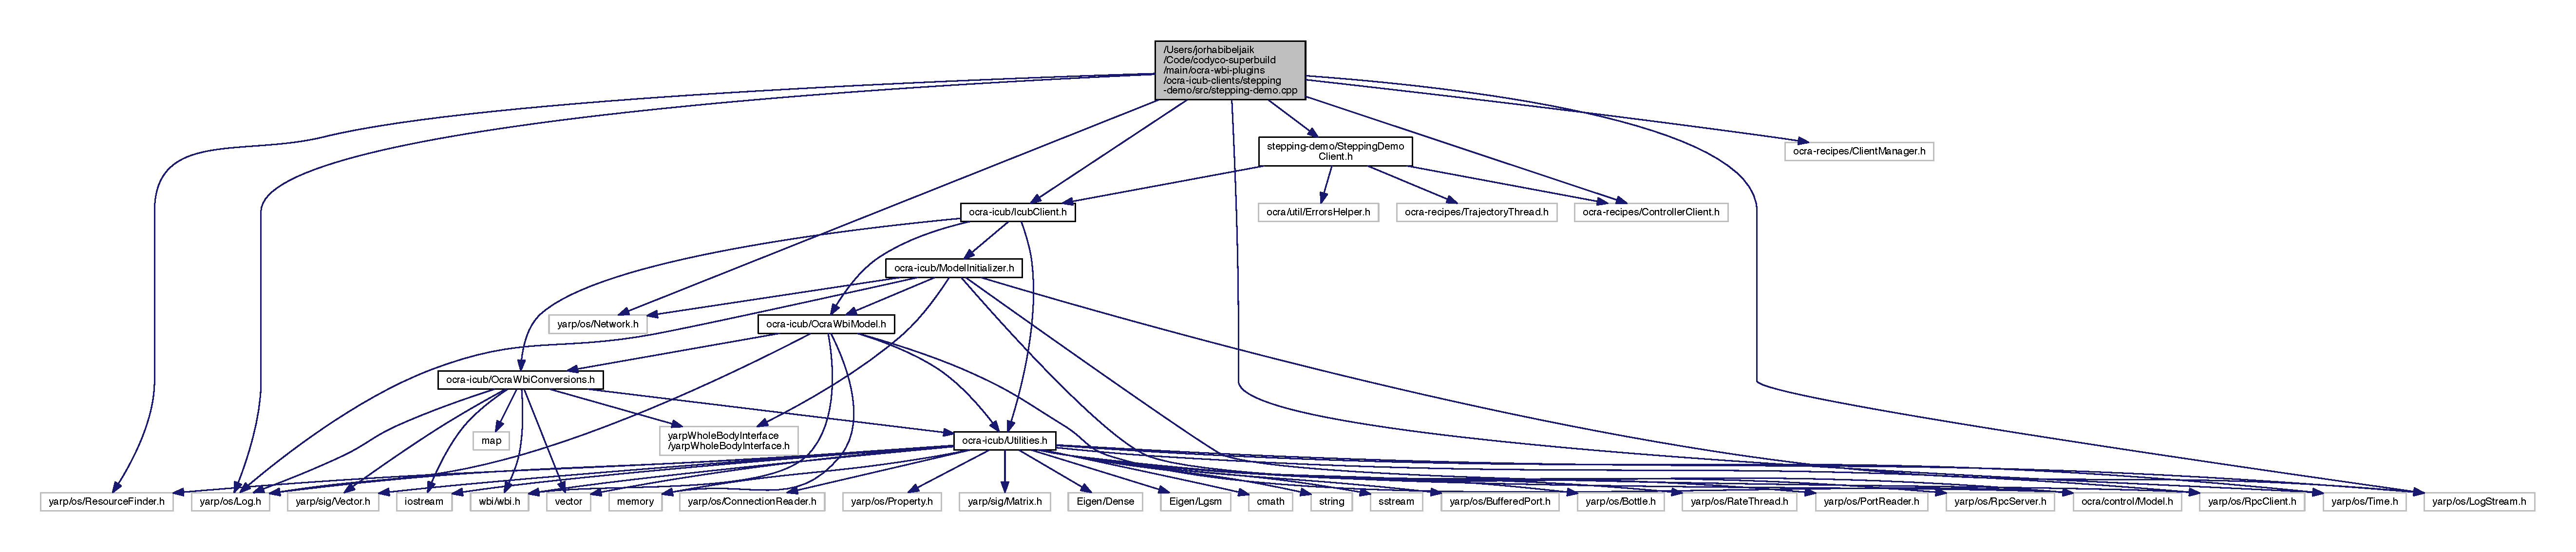
\includegraphics[width=350pt]{stepping-demo_8cpp__incl}
\end{center}
\end{figure}
\subsection*{Functions}
\begin{DoxyCompactItemize}
\item 
int \hyperlink{stepping-demo_8cpp_a0ddf1224851353fc92bfbff6f499fa97}{main} (int argc, char $\ast$argv\mbox{[}$\,$\mbox{]})
\end{DoxyCompactItemize}


\subsection{Detailed Description}
\begin{DoxyAuthor}{Author}
\href{http://www.ryanlober.com}{\tt Ryan Lober} 

\href{http://ahoarau.github.io}{\tt Antoine Hoarau} 
\end{DoxyAuthor}
\begin{DoxyDate}{Date}
Feb 2016 
\end{DoxyDate}
\begin{DoxyCopyright}{Copyright}
G\+NU General Public License. 
\end{DoxyCopyright}


\subsection{Function Documentation}
\hypertarget{stepping-demo_8cpp_a0ddf1224851353fc92bfbff6f499fa97}{}\label{stepping-demo_8cpp_a0ddf1224851353fc92bfbff6f499fa97} 
\index{stepping-\/demo.\+cpp@{stepping-\/demo.\+cpp}!main@{main}}
\index{main@{main}!stepping-\/demo.\+cpp@{stepping-\/demo.\+cpp}}
\subsubsection{\texorpdfstring{main()}{main()}}
{\footnotesize\ttfamily int main (\begin{DoxyParamCaption}\item[{int}]{argc,  }\item[{char $\ast$}]{argv\mbox{[}$\,$\mbox{]} }\end{DoxyParamCaption})}


\hypertarget{SteppingDemoClient_8cpp}{}\section{/\+Users/jorhabibeljaik/\+Code/codyco-\/superbuild/main/ocra-\/wbi-\/plugins/ocra-\/icub-\/clients/stepping-\/demo/src/\+Stepping\+Demo\+Client.cpp File Reference}
\label{SteppingDemoClient_8cpp}\index{/\+Users/jorhabibeljaik/\+Code/codyco-\/superbuild/main/ocra-\/wbi-\/plugins/ocra-\/icub-\/clients/stepping-\/demo/src/\+Stepping\+Demo\+Client.\+cpp@{/\+Users/jorhabibeljaik/\+Code/codyco-\/superbuild/main/ocra-\/wbi-\/plugins/ocra-\/icub-\/clients/stepping-\/demo/src/\+Stepping\+Demo\+Client.\+cpp}}
{\ttfamily \#include \char`\"{}stepping-\/demo/\+Stepping\+Demo\+Client.\+h\char`\"{}}\newline

\hypertarget{TaskOpsClient_8h}{}\section{/\+Users/jorhabibeljaik/\+Code/codyco-\/superbuild/main/ocra-\/wbi-\/plugins/ocra-\/icub-\/clients/task-\/operations-\/demo/include/task-\/operations-\/demo/\+Task\+Ops\+Client.h File Reference}
\label{TaskOpsClient_8h}\index{/\+Users/jorhabibeljaik/\+Code/codyco-\/superbuild/main/ocra-\/wbi-\/plugins/ocra-\/icub-\/clients/task-\/operations-\/demo/include/task-\/operations-\/demo/\+Task\+Ops\+Client.\+h@{/\+Users/jorhabibeljaik/\+Code/codyco-\/superbuild/main/ocra-\/wbi-\/plugins/ocra-\/icub-\/clients/task-\/operations-\/demo/include/task-\/operations-\/demo/\+Task\+Ops\+Client.\+h}}
{\ttfamily \#include $<$ocra-\/icub/\+Icub\+Client.\+h$>$}\newline
{\ttfamily \#include $<$ocra-\/recipes/\+Trajectory\+Thread.\+h$>$}\newline
{\ttfamily \#include $<$ocra-\/recipes/\+Controller\+Client.\+h$>$}\newline
Include dependency graph for Task\+Ops\+Client.\+h\+:
\nopagebreak
\begin{figure}[H]
\begin{center}
\leavevmode
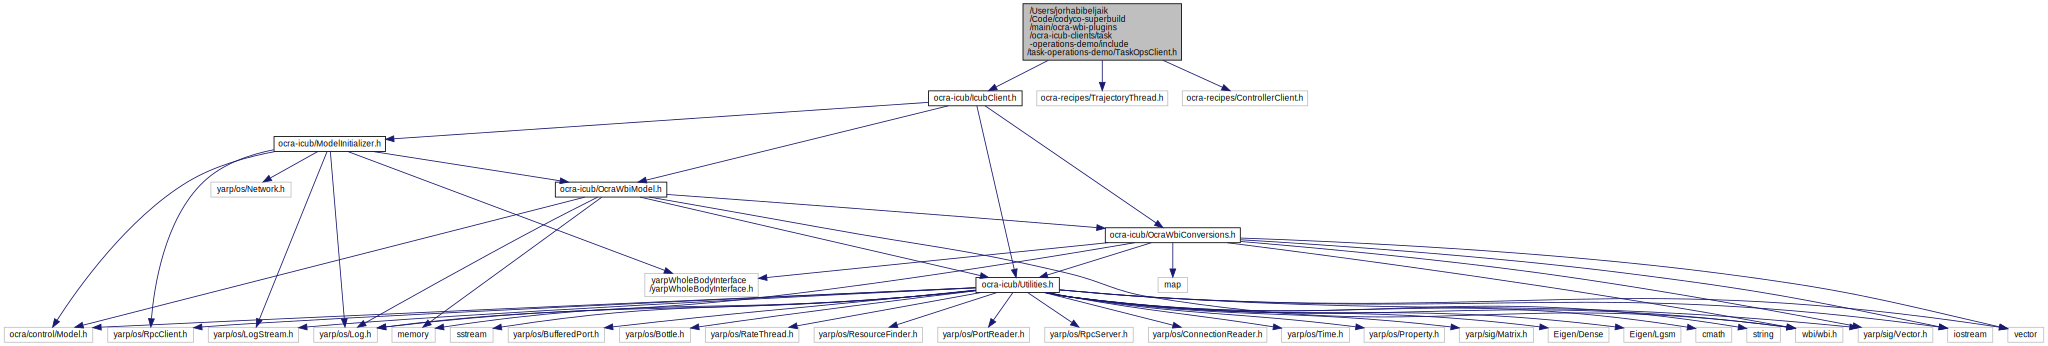
\includegraphics[width=350pt]{TaskOpsClient_8h__incl}
\end{center}
\end{figure}
This graph shows which files directly or indirectly include this file\+:
\nopagebreak
\begin{figure}[H]
\begin{center}
\leavevmode
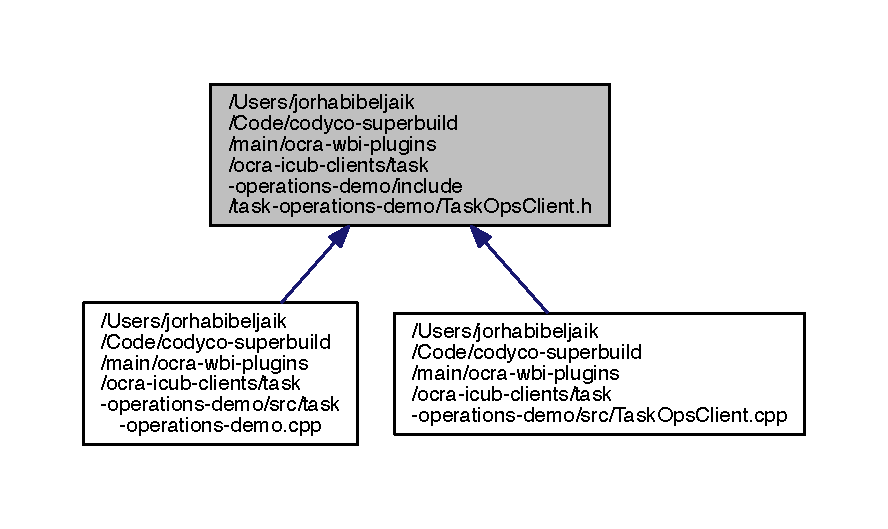
\includegraphics[width=350pt]{TaskOpsClient_8h__dep__incl}
\end{center}
\end{figure}
\subsection*{Classes}
\begin{DoxyCompactItemize}
\item 
class \hyperlink{classTaskOpsClient}{Task\+Ops\+Client}
\end{DoxyCompactItemize}
\subsection*{Enumerations}
\begin{DoxyCompactItemize}
\item 
enum \hyperlink{TaskOpsClient_8h_a0140057ae3fbe1db5f5c418dfc67d9db}{T\+H\+I\+N\+G\+S\+\_\+\+T\+O\+\_\+\+DO} \{ \newline
\hyperlink{TaskOpsClient_8h_a0140057ae3fbe1db5f5c418dfc67d9dbaf831abed77e2c76cacc256b8b16f2b2a}{R\+E\+M\+O\+V\+E\+\_\+\+T\+A\+SK}, 
\hyperlink{TaskOpsClient_8h_a0140057ae3fbe1db5f5c418dfc67d9dba6aa666a68fed72da5438e0ef9b7cba8f}{A\+D\+D\+\_\+\+N\+E\+W\+\_\+\+T\+A\+SK}, 
\hyperlink{TaskOpsClient_8h_a0140057ae3fbe1db5f5c418dfc67d9dba8ffc9eba853106ab798ee2a0c5763d1b}{A\+D\+D\+\_\+\+E\+X\+I\+S\+T\+I\+N\+G\+\_\+\+T\+A\+SK}, 
\hyperlink{TaskOpsClient_8h_a0140057ae3fbe1db5f5c418dfc67d9dba7eaf30861bc723f003ea1a8e4a7a4977}{A\+D\+D\+\_\+\+E\+X\+I\+S\+T\+I\+N\+G\+\_\+\+T\+A\+S\+K\+\_\+\+N\+O\+\_\+\+O\+V\+E\+R\+W\+R\+I\+TE}, 
\newline
\hyperlink{TaskOpsClient_8h_a0140057ae3fbe1db5f5c418dfc67d9dbacfe24a7b308a82835c8a9a9a89bc4ca2}{N\+O\+T\+H\+I\+NG}
 \}
\end{DoxyCompactItemize}


\subsection{Enumeration Type Documentation}
\hypertarget{TaskOpsClient_8h_a0140057ae3fbe1db5f5c418dfc67d9db}{}\label{TaskOpsClient_8h_a0140057ae3fbe1db5f5c418dfc67d9db} 
\index{Task\+Ops\+Client.\+h@{Task\+Ops\+Client.\+h}!T\+H\+I\+N\+G\+S\+\_\+\+T\+O\+\_\+\+DO@{T\+H\+I\+N\+G\+S\+\_\+\+T\+O\+\_\+\+DO}}
\index{T\+H\+I\+N\+G\+S\+\_\+\+T\+O\+\_\+\+DO@{T\+H\+I\+N\+G\+S\+\_\+\+T\+O\+\_\+\+DO}!Task\+Ops\+Client.\+h@{Task\+Ops\+Client.\+h}}
\subsubsection{\texorpdfstring{T\+H\+I\+N\+G\+S\+\_\+\+T\+O\+\_\+\+DO}{THINGS\_TO\_DO}}
{\footnotesize\ttfamily enum \hyperlink{TaskOpsClient_8h_a0140057ae3fbe1db5f5c418dfc67d9db}{T\+H\+I\+N\+G\+S\+\_\+\+T\+O\+\_\+\+DO}}

\begin{DoxyEnumFields}{Enumerator}
\raisebox{\heightof{T}}[0pt][0pt]{\index{R\+E\+M\+O\+V\+E\+\_\+\+T\+A\+SK@{R\+E\+M\+O\+V\+E\+\_\+\+T\+A\+SK}!Task\+Ops\+Client.\+h@{Task\+Ops\+Client.\+h}}\index{Task\+Ops\+Client.\+h@{Task\+Ops\+Client.\+h}!R\+E\+M\+O\+V\+E\+\_\+\+T\+A\+SK@{R\+E\+M\+O\+V\+E\+\_\+\+T\+A\+SK}}}\hypertarget{TaskOpsClient_8h_a0140057ae3fbe1db5f5c418dfc67d9dbaf831abed77e2c76cacc256b8b16f2b2a}{}\label{TaskOpsClient_8h_a0140057ae3fbe1db5f5c418dfc67d9dbaf831abed77e2c76cacc256b8b16f2b2a} 
R\+E\+M\+O\+V\+E\+\_\+\+T\+A\+SK&\\
\hline

\raisebox{\heightof{T}}[0pt][0pt]{\index{A\+D\+D\+\_\+\+N\+E\+W\+\_\+\+T\+A\+SK@{A\+D\+D\+\_\+\+N\+E\+W\+\_\+\+T\+A\+SK}!Task\+Ops\+Client.\+h@{Task\+Ops\+Client.\+h}}\index{Task\+Ops\+Client.\+h@{Task\+Ops\+Client.\+h}!A\+D\+D\+\_\+\+N\+E\+W\+\_\+\+T\+A\+SK@{A\+D\+D\+\_\+\+N\+E\+W\+\_\+\+T\+A\+SK}}}\hypertarget{TaskOpsClient_8h_a0140057ae3fbe1db5f5c418dfc67d9dba6aa666a68fed72da5438e0ef9b7cba8f}{}\label{TaskOpsClient_8h_a0140057ae3fbe1db5f5c418dfc67d9dba6aa666a68fed72da5438e0ef9b7cba8f} 
A\+D\+D\+\_\+\+N\+E\+W\+\_\+\+T\+A\+SK&\\
\hline

\raisebox{\heightof{T}}[0pt][0pt]{\index{A\+D\+D\+\_\+\+E\+X\+I\+S\+T\+I\+N\+G\+\_\+\+T\+A\+SK@{A\+D\+D\+\_\+\+E\+X\+I\+S\+T\+I\+N\+G\+\_\+\+T\+A\+SK}!Task\+Ops\+Client.\+h@{Task\+Ops\+Client.\+h}}\index{Task\+Ops\+Client.\+h@{Task\+Ops\+Client.\+h}!A\+D\+D\+\_\+\+E\+X\+I\+S\+T\+I\+N\+G\+\_\+\+T\+A\+SK@{A\+D\+D\+\_\+\+E\+X\+I\+S\+T\+I\+N\+G\+\_\+\+T\+A\+SK}}}\hypertarget{TaskOpsClient_8h_a0140057ae3fbe1db5f5c418dfc67d9dba8ffc9eba853106ab798ee2a0c5763d1b}{}\label{TaskOpsClient_8h_a0140057ae3fbe1db5f5c418dfc67d9dba8ffc9eba853106ab798ee2a0c5763d1b} 
A\+D\+D\+\_\+\+E\+X\+I\+S\+T\+I\+N\+G\+\_\+\+T\+A\+SK&\\
\hline

\raisebox{\heightof{T}}[0pt][0pt]{\index{A\+D\+D\+\_\+\+E\+X\+I\+S\+T\+I\+N\+G\+\_\+\+T\+A\+S\+K\+\_\+\+N\+O\+\_\+\+O\+V\+E\+R\+W\+R\+I\+TE@{A\+D\+D\+\_\+\+E\+X\+I\+S\+T\+I\+N\+G\+\_\+\+T\+A\+S\+K\+\_\+\+N\+O\+\_\+\+O\+V\+E\+R\+W\+R\+I\+TE}!Task\+Ops\+Client.\+h@{Task\+Ops\+Client.\+h}}\index{Task\+Ops\+Client.\+h@{Task\+Ops\+Client.\+h}!A\+D\+D\+\_\+\+E\+X\+I\+S\+T\+I\+N\+G\+\_\+\+T\+A\+S\+K\+\_\+\+N\+O\+\_\+\+O\+V\+E\+R\+W\+R\+I\+TE@{A\+D\+D\+\_\+\+E\+X\+I\+S\+T\+I\+N\+G\+\_\+\+T\+A\+S\+K\+\_\+\+N\+O\+\_\+\+O\+V\+E\+R\+W\+R\+I\+TE}}}\hypertarget{TaskOpsClient_8h_a0140057ae3fbe1db5f5c418dfc67d9dba7eaf30861bc723f003ea1a8e4a7a4977}{}\label{TaskOpsClient_8h_a0140057ae3fbe1db5f5c418dfc67d9dba7eaf30861bc723f003ea1a8e4a7a4977} 
A\+D\+D\+\_\+\+E\+X\+I\+S\+T\+I\+N\+G\+\_\+\+T\+A\+S\+K\+\_\+\+N\+O\+\_\+\+O\+V\+E\+R\+W\+R\+I\+TE&\\
\hline

\raisebox{\heightof{T}}[0pt][0pt]{\index{N\+O\+T\+H\+I\+NG@{N\+O\+T\+H\+I\+NG}!Task\+Ops\+Client.\+h@{Task\+Ops\+Client.\+h}}\index{Task\+Ops\+Client.\+h@{Task\+Ops\+Client.\+h}!N\+O\+T\+H\+I\+NG@{N\+O\+T\+H\+I\+NG}}}\hypertarget{TaskOpsClient_8h_a0140057ae3fbe1db5f5c418dfc67d9dbacfe24a7b308a82835c8a9a9a89bc4ca2}{}\label{TaskOpsClient_8h_a0140057ae3fbe1db5f5c418dfc67d9dbacfe24a7b308a82835c8a9a9a89bc4ca2} 
N\+O\+T\+H\+I\+NG&\\
\hline

\end{DoxyEnumFields}

\hypertarget{task-operations-demo_8cpp}{}\section{/\+Users/jorhabibeljaik/\+Code/codyco-\/superbuild/main/ocra-\/wbi-\/plugins/ocra-\/icub-\/clients/task-\/operations-\/demo/src/task-\/operations-\/demo.cpp File Reference}
\label{task-operations-demo_8cpp}\index{/\+Users/jorhabibeljaik/\+Code/codyco-\/superbuild/main/ocra-\/wbi-\/plugins/ocra-\/icub-\/clients/task-\/operations-\/demo/src/task-\/operations-\/demo.\+cpp@{/\+Users/jorhabibeljaik/\+Code/codyco-\/superbuild/main/ocra-\/wbi-\/plugins/ocra-\/icub-\/clients/task-\/operations-\/demo/src/task-\/operations-\/demo.\+cpp}}
{\ttfamily \#include $<$yarp/os/\+Resource\+Finder.\+h$>$}\newline
{\ttfamily \#include $<$yarp/os/\+Network.\+h$>$}\newline
{\ttfamily \#include $<$yarp/os/\+Log.\+h$>$}\newline
{\ttfamily \#include $<$yarp/os/\+Log\+Stream.\+h$>$}\newline
{\ttfamily \#include $<$yarp/os/\+Time.\+h$>$}\newline
{\ttfamily \#include \char`\"{}task-\/operations-\/demo/\+Task\+Ops\+Client.\+h\char`\"{}}\newline
{\ttfamily \#include $<$ocra-\/icub/\+Icub\+Client.\+h$>$}\newline
{\ttfamily \#include $<$ocra-\/recipes/\+Controller\+Client.\+h$>$}\newline
{\ttfamily \#include $<$ocra-\/recipes/\+Client\+Manager.\+h$>$}\newline
Include dependency graph for task-\/operations-\/demo.cpp\+:\nopagebreak
\begin{figure}[H]
\begin{center}
\leavevmode
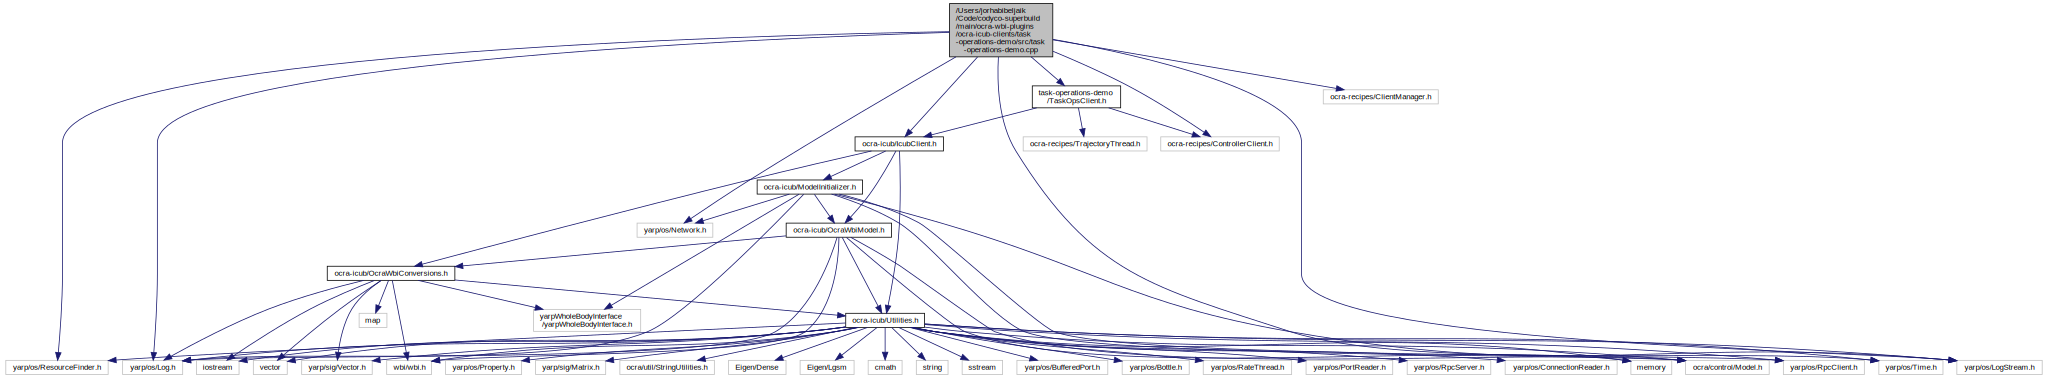
\includegraphics[width=350pt]{task-operations-demo_8cpp__incl}
\end{center}
\end{figure}
\subsection*{Functions}
\begin{DoxyCompactItemize}
\item 
int \hyperlink{task-operations-demo_8cpp_a0ddf1224851353fc92bfbff6f499fa97}{main} (int argc, char $\ast$argv\mbox{[}$\,$\mbox{]})
\end{DoxyCompactItemize}


\subsection{Function Documentation}
\hypertarget{task-operations-demo_8cpp_a0ddf1224851353fc92bfbff6f499fa97}{}\label{task-operations-demo_8cpp_a0ddf1224851353fc92bfbff6f499fa97} 
\index{task-\/operations-\/demo.\+cpp@{task-\/operations-\/demo.\+cpp}!main@{main}}
\index{main@{main}!task-\/operations-\/demo.\+cpp@{task-\/operations-\/demo.\+cpp}}
\subsubsection{\texorpdfstring{main()}{main()}}
{\footnotesize\ttfamily int main (\begin{DoxyParamCaption}\item[{int}]{argc,  }\item[{char $\ast$}]{argv\mbox{[}$\,$\mbox{]} }\end{DoxyParamCaption})}


\hypertarget{TaskOpsClient_8cpp}{}\section{/\+Users/jorhabibeljaik/\+Code/codyco-\/superbuild/main/ocra-\/wbi-\/plugins/ocra-\/icub-\/clients/task-\/operations-\/demo/src/\+Task\+Ops\+Client.cpp File Reference}
\label{TaskOpsClient_8cpp}\index{/\+Users/jorhabibeljaik/\+Code/codyco-\/superbuild/main/ocra-\/wbi-\/plugins/ocra-\/icub-\/clients/task-\/operations-\/demo/src/\+Task\+Ops\+Client.\+cpp@{/\+Users/jorhabibeljaik/\+Code/codyco-\/superbuild/main/ocra-\/wbi-\/plugins/ocra-\/icub-\/clients/task-\/operations-\/demo/src/\+Task\+Ops\+Client.\+cpp}}
{\ttfamily \#include \char`\"{}task-\/operations-\/demo/\+Task\+Ops\+Client.\+h\char`\"{}}\newline
Include dependency graph for Task\+Ops\+Client.\+cpp\+:\nopagebreak
\begin{figure}[H]
\begin{center}
\leavevmode
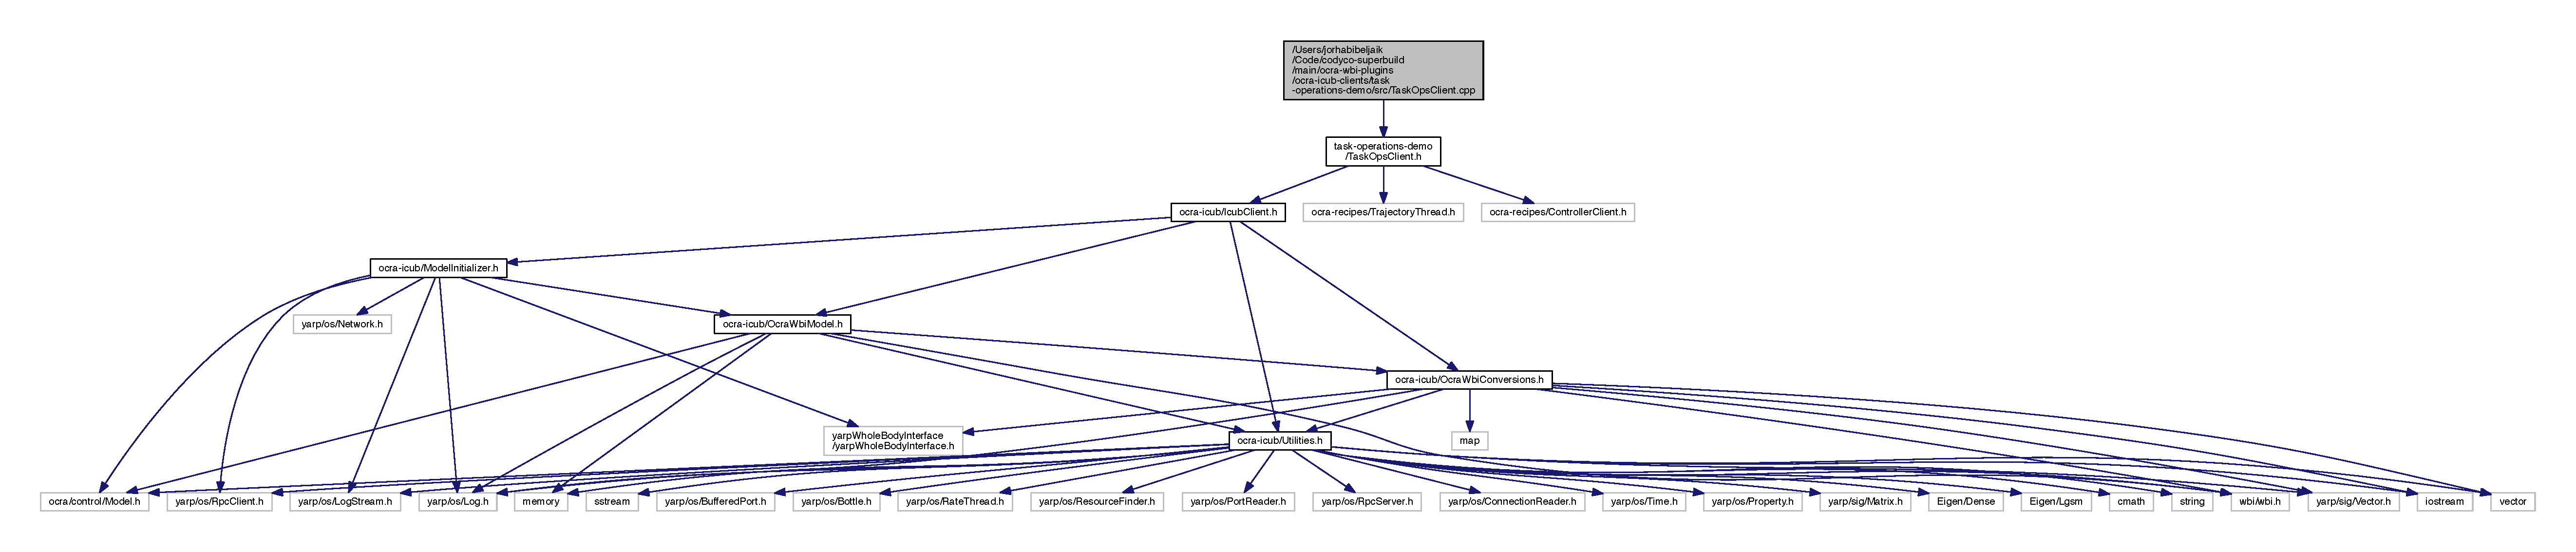
\includegraphics[width=350pt]{TaskOpsClient_8cpp__incl}
\end{center}
\end{figure}

\hypertarget{IcubControllerServer_8h}{}\section{/\+Users/jorhabibeljaik/\+Code/codyco-\/superbuild/main/ocra-\/wbi-\/plugins/ocra-\/icub-\/server/include/ocra-\/icub-\/server/\+Icub\+Controller\+Server.h File Reference}
\label{IcubControllerServer_8h}\index{/\+Users/jorhabibeljaik/\+Code/codyco-\/superbuild/main/ocra-\/wbi-\/plugins/ocra-\/icub-\/server/include/ocra-\/icub-\/server/\+Icub\+Controller\+Server.\+h@{/\+Users/jorhabibeljaik/\+Code/codyco-\/superbuild/main/ocra-\/wbi-\/plugins/ocra-\/icub-\/server/include/ocra-\/icub-\/server/\+Icub\+Controller\+Server.\+h}}
{\ttfamily \#include $<$wbi/wbi.\+h$>$}\newline
{\ttfamily \#include $<$ocra-\/recipes/\+Controller\+Server.\+h$>$}\newline
{\ttfamily \#include $<$Eigen/\+Dense$>$}\newline
{\ttfamily \#include $<$ocra-\/icub/\+Ocra\+Wbi\+Model.\+h$>$}\newline
{\ttfamily \#include $<$i\+Dyn\+Tree/\+Estimation/\+Simple\+Legged\+Odometry.\+h$>$}\newline
{\ttfamily \#include $<$ocra/util/\+Errors\+Helper.\+h$>$}\newline
Include dependency graph for Icub\+Controller\+Server.\+h\+:
\nopagebreak
\begin{figure}[H]
\begin{center}
\leavevmode
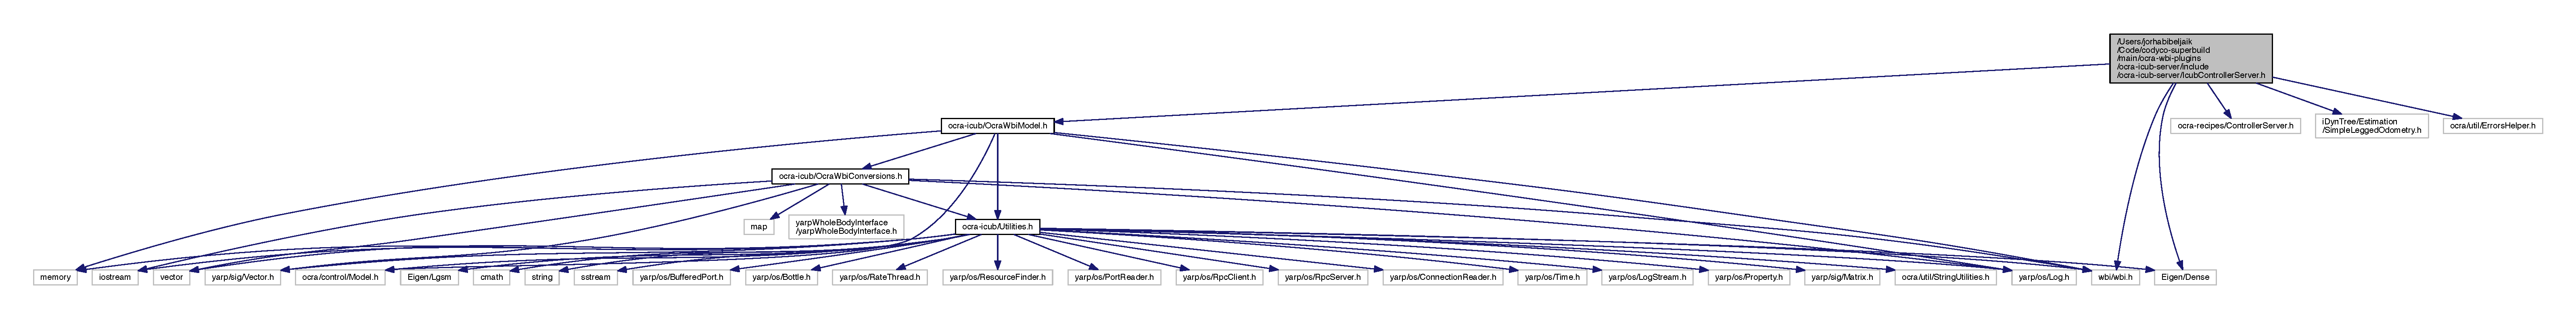
\includegraphics[width=350pt]{IcubControllerServer_8h__incl}
\end{center}
\end{figure}
This graph shows which files directly or indirectly include this file\+:
\nopagebreak
\begin{figure}[H]
\begin{center}
\leavevmode
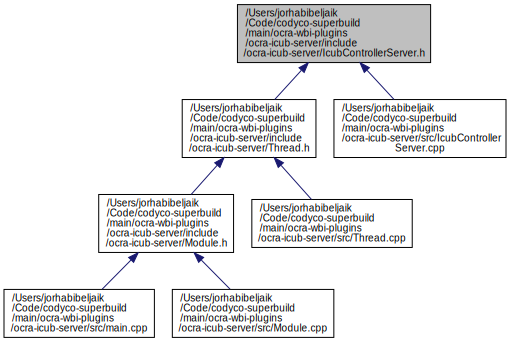
\includegraphics[width=350pt]{IcubControllerServer_8h__dep__incl}
\end{center}
\end{figure}
\subsection*{Classes}
\begin{DoxyCompactItemize}
\item 
class \hyperlink{classIcubControllerServer}{Icub\+Controller\+Server}
\end{DoxyCompactItemize}

\hypertarget{Module_8h}{}\section{/\+Users/jorhabibeljaik/\+Code/codyco-\/superbuild/main/ocra-\/wbi-\/plugins/ocra-\/icub-\/server/include/ocra-\/icub-\/server/\+Module.h File Reference}
\label{Module_8h}\index{/\+Users/jorhabibeljaik/\+Code/codyco-\/superbuild/main/ocra-\/wbi-\/plugins/ocra-\/icub-\/server/include/ocra-\/icub-\/server/\+Module.\+h@{/\+Users/jorhabibeljaik/\+Code/codyco-\/superbuild/main/ocra-\/wbi-\/plugins/ocra-\/icub-\/server/include/ocra-\/icub-\/server/\+Module.\+h}}


\hyperlink{classModule}{Module} class for the controller server.  


{\ttfamily \#include $<$iostream$>$}\newline
{\ttfamily \#include $<$memory$>$}\newline
{\ttfamily \#include $<$algorithm$>$}\newline
{\ttfamily \#include $<$locale$>$}\newline
{\ttfamily \#include $<$yarp/os/\+R\+F\+Module.\+h$>$}\newline
{\ttfamily \#include $<$yarp\+Whole\+Body\+Interface/yarp\+Whole\+Body\+Interface.\+h$>$}\newline
{\ttfamily \#include \char`\"{}ocra-\/icub-\/server/\+Thread.\+h\char`\"{}}\newline
{\ttfamily \#include \char`\"{}ocra-\/icub/\+Utilities.\+h\char`\"{}}\newline
\subsection*{Classes}
\begin{DoxyCompactItemize}
\item 
class \hyperlink{classModule}{Module}
\begin{DoxyCompactList}\small\item\em The controller module which launches the controller thread. \end{DoxyCompactList}\end{DoxyCompactItemize}


\subsection{Detailed Description}
\hyperlink{classModule}{Module} class for the controller server. 

\begin{DoxyAuthor}{Author}
\href{http://www.ryanlober.com}{\tt Ryan Lober} 

\href{http://ahoarau.github.io}{\tt Antoine Hoarau} 
\end{DoxyAuthor}
\begin{DoxyDate}{Date}
Feb 2016 
\end{DoxyDate}
\begin{DoxyCopyright}{Copyright}
G\+NU General Public License. 
\end{DoxyCopyright}

\hypertarget{Thread_8h}{}\section{/\+Users/jorhabibeljaik/\+Code/codyco-\/superbuild/main/ocra-\/wbi-\/plugins/ocra-\/icub-\/server/include/ocra-\/icub-\/server/\+Thread.h File Reference}
\label{Thread_8h}\index{/\+Users/jorhabibeljaik/\+Code/codyco-\/superbuild/main/ocra-\/wbi-\/plugins/ocra-\/icub-\/server/include/ocra-\/icub-\/server/\+Thread.\+h@{/\+Users/jorhabibeljaik/\+Code/codyco-\/superbuild/main/ocra-\/wbi-\/plugins/ocra-\/icub-\/server/include/ocra-\/icub-\/server/\+Thread.\+h}}


The thread class for the controller server.  


{\ttfamily \#include $<$yarp\+Whole\+Body\+Interface/yarp\+Whole\+Body\+Interface.\+h$>$}\newline
{\ttfamily \#include $<$wbi/wbi.\+h$>$}\newline
{\ttfamily \#include $<$ocra-\/icub-\/server/\+Icub\+Controller\+Server.\+h$>$}\newline
{\ttfamily \#include $<$ocra-\/icub/\+Utilities.\+h$>$}\newline
{\ttfamily \#include $<$ocra/util/\+Errors\+Helper.\+h$>$}\newline
{\ttfamily \#include $<$yarp/os/\+Bottle.\+h$>$}\newline
{\ttfamily \#include $<$yarp/os/\+Rpc\+Server.\+h$>$}\newline
{\ttfamily \#include $<$yarp/os/\+Connection\+Reader.\+h$>$}\newline
{\ttfamily \#include $<$yarp/os/\+Time.\+h$>$}\newline
{\ttfamily \#include $<$sstream$>$}\newline
{\ttfamily \#include $<$string$>$}\newline
{\ttfamily \#include $<$i\+Dyn\+Tree/\+Estimation/\+Simple\+Legged\+Odometry.\+h$>$}\newline
Include dependency graph for Thread.\+h\+:\nopagebreak
\begin{figure}[H]
\begin{center}
\leavevmode
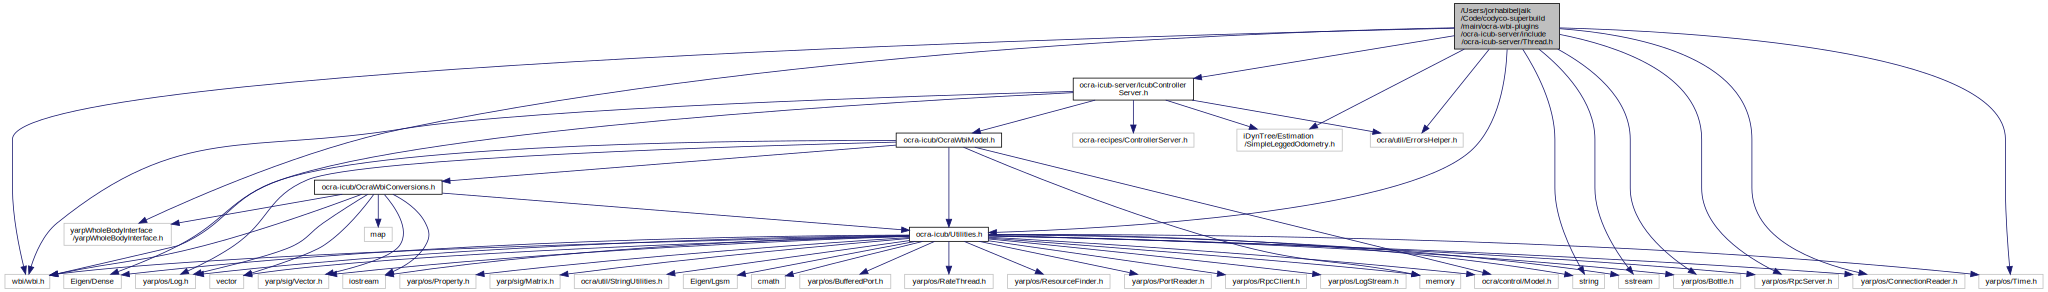
\includegraphics[width=350pt]{Thread_8h__incl}
\end{center}
\end{figure}
This graph shows which files directly or indirectly include this file\+:\nopagebreak
\begin{figure}[H]
\begin{center}
\leavevmode
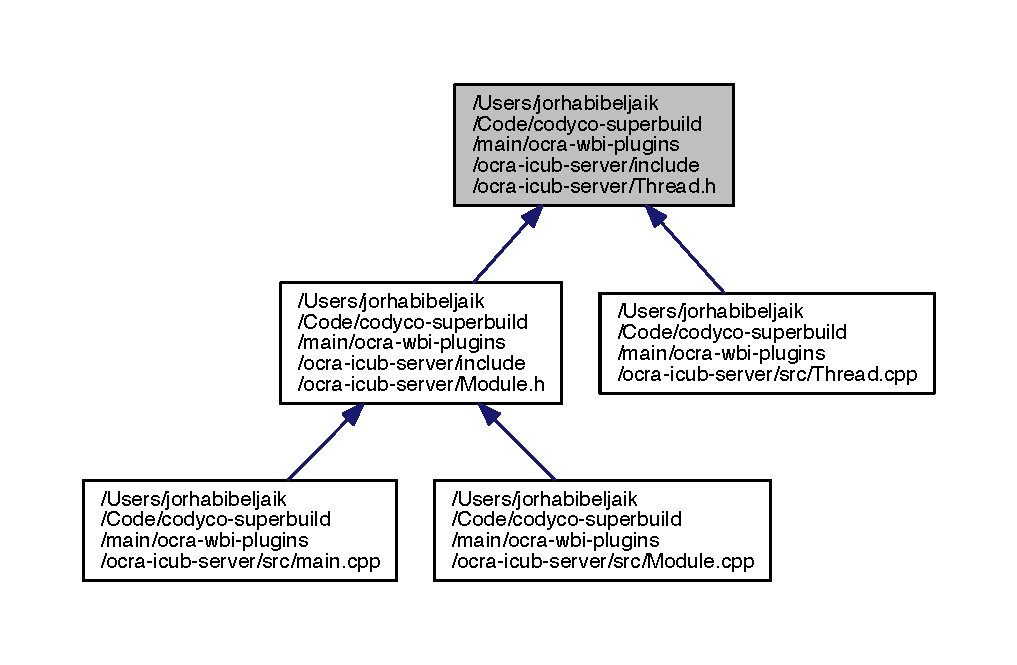
\includegraphics[width=350pt]{Thread_8h__dep__incl}
\end{center}
\end{figure}
\subsection*{Classes}
\begin{DoxyCompactItemize}
\item 
class \hyperlink{classOcraControllerOptions}{Ocra\+Controller\+Options}
\item 
class \hyperlink{classThread}{Thread}
\begin{DoxyCompactList}\small\item\em The meat and potatoes of the controller server. \end{DoxyCompactList}\item 
class \hyperlink{classThread_1_1ControllerRpcServerCallback}{Thread\+::\+Controller\+Rpc\+Server\+Callback}
\begin{DoxyCompactList}\small\item\em A callback function which binds the rpc server port opened in the contoller server module to the controller thread\textquotesingle{}s parsing function. \end{DoxyCompactList}\item 
class \hyperlink{classThread_1_1DebugRpcServerCallback}{Thread\+::\+Debug\+Rpc\+Server\+Callback}
\begin{DoxyCompactList}\small\item\em A callback function which binds the rpc server port opened in the contoller server module to the controller thread\textquotesingle{}s parsing function. \end{DoxyCompactList}\end{DoxyCompactItemize}


\subsection{Detailed Description}
The thread class for the controller server. 

\begin{DoxyAuthor}{Author}
\href{http://www.ryanlober.com}{\tt Ryan Lober} 

\href{http://ahoarau.github.io}{\tt Antoine Hoarau} 
\end{DoxyAuthor}
\begin{DoxyDate}{Date}
Feb 2016 
\end{DoxyDate}
\begin{DoxyCopyright}{Copyright}
G\+NU General Public License. 
\end{DoxyCopyright}

\hypertarget{IcubControllerServer_8cpp}{}\section{/\+Users/jorhabibeljaik/\+Code/codyco-\/superbuild/main/ocra-\/wbi-\/plugins/ocra-\/icub-\/server/src/\+Icub\+Controller\+Server.cpp File Reference}
\label{IcubControllerServer_8cpp}\index{/\+Users/jorhabibeljaik/\+Code/codyco-\/superbuild/main/ocra-\/wbi-\/plugins/ocra-\/icub-\/server/src/\+Icub\+Controller\+Server.\+cpp@{/\+Users/jorhabibeljaik/\+Code/codyco-\/superbuild/main/ocra-\/wbi-\/plugins/ocra-\/icub-\/server/src/\+Icub\+Controller\+Server.\+cpp}}
{\ttfamily \#include $<$ocra-\/icub-\/server/\+Icub\+Controller\+Server.\+h$>$}\newline
Include dependency graph for Icub\+Controller\+Server.\+cpp\+:
\nopagebreak
\begin{figure}[H]
\begin{center}
\leavevmode
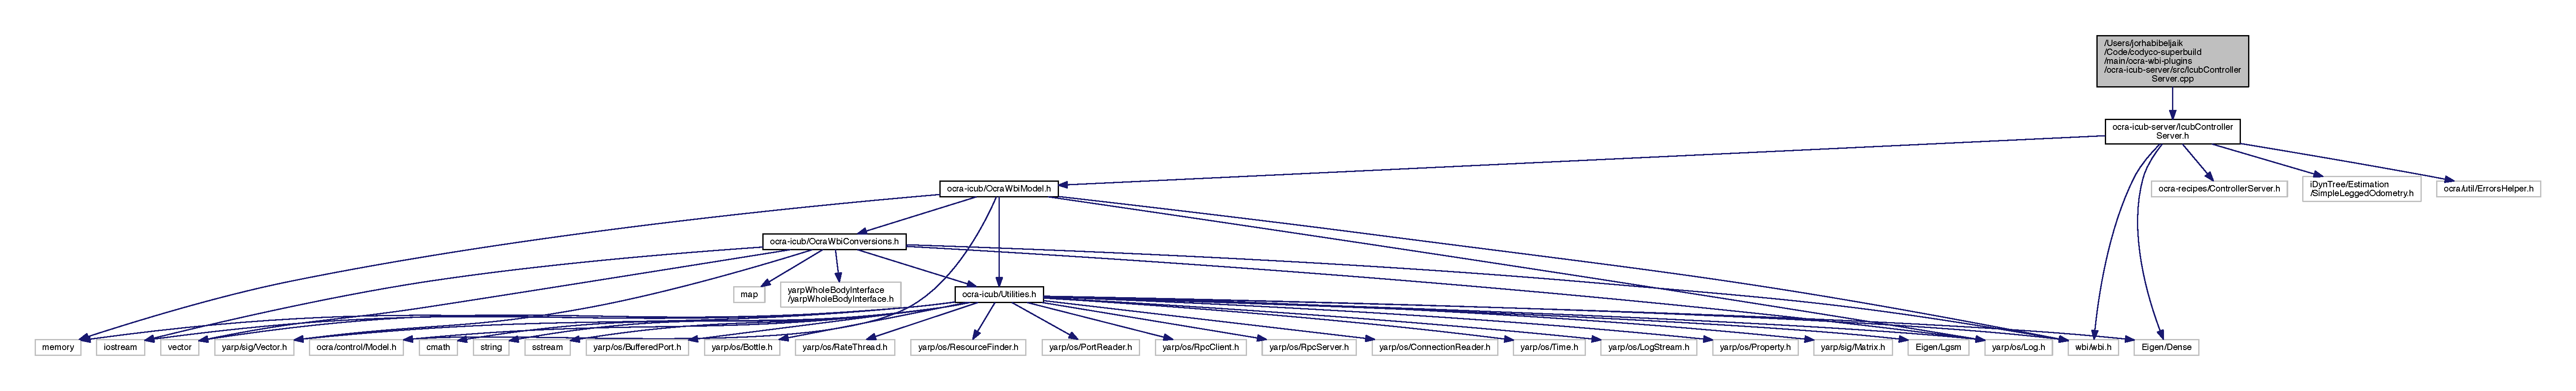
\includegraphics[width=350pt]{IcubControllerServer_8cpp__incl}
\end{center}
\end{figure}

\hypertarget{main_8cpp}{}\section{/\+Users/jorhabibeljaik/\+Code/codyco-\/superbuild/main/ocra-\/wbi-\/plugins/ocra-\/icub-\/server/src/main.cpp File Reference}
\label{main_8cpp}\index{/\+Users/jorhabibeljaik/\+Code/codyco-\/superbuild/main/ocra-\/wbi-\/plugins/ocra-\/icub-\/server/src/main.\+cpp@{/\+Users/jorhabibeljaik/\+Code/codyco-\/superbuild/main/ocra-\/wbi-\/plugins/ocra-\/icub-\/server/src/main.\+cpp}}


Basically just launches the server module which then launches the server thread. (...it\textquotesingle{}s a dream within a dream)  


{\ttfamily \#include $<$yarp/os/\+Resource\+Finder.\+h$>$}\newline
{\ttfamily \#include $<$yarp/os/\+Network.\+h$>$}\newline
{\ttfamily \#include $<$yarp/os/\+Log.\+h$>$}\newline
{\ttfamily \#include $<$ocra-\/icub-\/server/\+Module.\+h$>$}\newline
Include dependency graph for main.\+cpp\+:\nopagebreak
\begin{figure}[H]
\begin{center}
\leavevmode
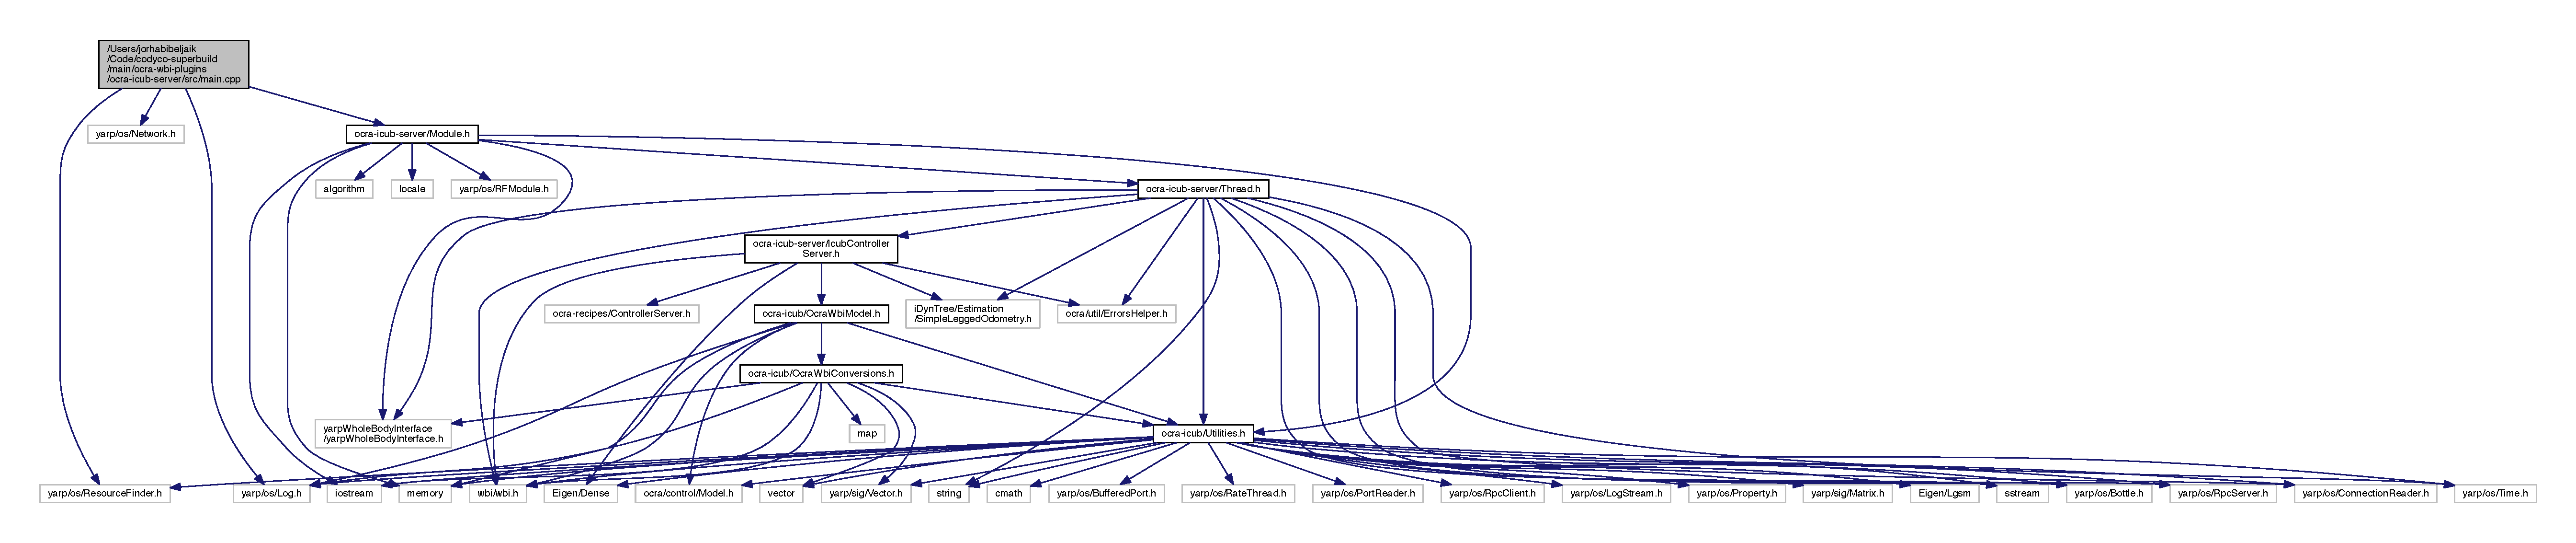
\includegraphics[width=350pt]{main_8cpp__incl}
\end{center}
\end{figure}
\subsection*{Macros}
\begin{DoxyCompactItemize}
\item 
\#define \hyperlink{main_8cpp_aacf7b13861a4ce37b8dec1979eb6450c}{D\+E\+F\+A\+U\+L\+T\+\_\+\+Y\+A\+R\+P\+\_\+\+C\+O\+N\+T\+E\+XT}~\char`\"{}ocra-\/icub-\/server\char`\"{}
\end{DoxyCompactItemize}
\subsection*{Functions}
\begin{DoxyCompactItemize}
\item 
int \hyperlink{main_8cpp_a0ddf1224851353fc92bfbff6f499fa97}{main} (int argc, char $\ast$argv\mbox{[}$\,$\mbox{]})
\end{DoxyCompactItemize}


\subsection{Detailed Description}
Basically just launches the server module which then launches the server thread. (...it\textquotesingle{}s a dream within a dream) 

\begin{DoxyAuthor}{Author}
\href{http://www.ryanlober.com}{\tt Ryan Lober} 

\href{http://ahoarau.github.io}{\tt Antoine Hoarau} 
\end{DoxyAuthor}
\begin{DoxyDate}{Date}
Feb 2016 
\end{DoxyDate}
\begin{DoxyCopyright}{Copyright}
G\+NU General Public License. 
\end{DoxyCopyright}


\subsection{Macro Definition Documentation}
\hypertarget{main_8cpp_aacf7b13861a4ce37b8dec1979eb6450c}{}\label{main_8cpp_aacf7b13861a4ce37b8dec1979eb6450c} 
\index{main.\+cpp@{main.\+cpp}!D\+E\+F\+A\+U\+L\+T\+\_\+\+Y\+A\+R\+P\+\_\+\+C\+O\+N\+T\+E\+XT@{D\+E\+F\+A\+U\+L\+T\+\_\+\+Y\+A\+R\+P\+\_\+\+C\+O\+N\+T\+E\+XT}}
\index{D\+E\+F\+A\+U\+L\+T\+\_\+\+Y\+A\+R\+P\+\_\+\+C\+O\+N\+T\+E\+XT@{D\+E\+F\+A\+U\+L\+T\+\_\+\+Y\+A\+R\+P\+\_\+\+C\+O\+N\+T\+E\+XT}!main.\+cpp@{main.\+cpp}}
\subsubsection{\texorpdfstring{D\+E\+F\+A\+U\+L\+T\+\_\+\+Y\+A\+R\+P\+\_\+\+C\+O\+N\+T\+E\+XT}{DEFAULT\_YARP\_CONTEXT}}
{\footnotesize\ttfamily \#define D\+E\+F\+A\+U\+L\+T\+\_\+\+Y\+A\+R\+P\+\_\+\+C\+O\+N\+T\+E\+XT~\char`\"{}ocra-\/icub-\/server\char`\"{}}



\subsection{Function Documentation}
\hypertarget{main_8cpp_a0ddf1224851353fc92bfbff6f499fa97}{}\label{main_8cpp_a0ddf1224851353fc92bfbff6f499fa97} 
\index{main.\+cpp@{main.\+cpp}!main@{main}}
\index{main@{main}!main.\+cpp@{main.\+cpp}}
\subsubsection{\texorpdfstring{main()}{main()}}
{\footnotesize\ttfamily int main (\begin{DoxyParamCaption}\item[{int}]{argc,  }\item[{char $\ast$}]{argv\mbox{[}$\,$\mbox{]} }\end{DoxyParamCaption})}


\hypertarget{Module_8cpp}{}\section{/\+Users/jorhabibeljaik/\+Code/codyco-\/superbuild/main/ocra-\/wbi-\/plugins/ocra-\/icub-\/server/src/\+Module.cpp File Reference}
\label{Module_8cpp}\index{/\+Users/jorhabibeljaik/\+Code/codyco-\/superbuild/main/ocra-\/wbi-\/plugins/ocra-\/icub-\/server/src/\+Module.\+cpp@{/\+Users/jorhabibeljaik/\+Code/codyco-\/superbuild/main/ocra-\/wbi-\/plugins/ocra-\/icub-\/server/src/\+Module.\+cpp}}
{\ttfamily \#include \char`\"{}ocra-\/icub-\/server/\+Module.\+h\char`\"{}}\newline
Include dependency graph for Module.\+cpp\+:
\nopagebreak
\begin{figure}[H]
\begin{center}
\leavevmode
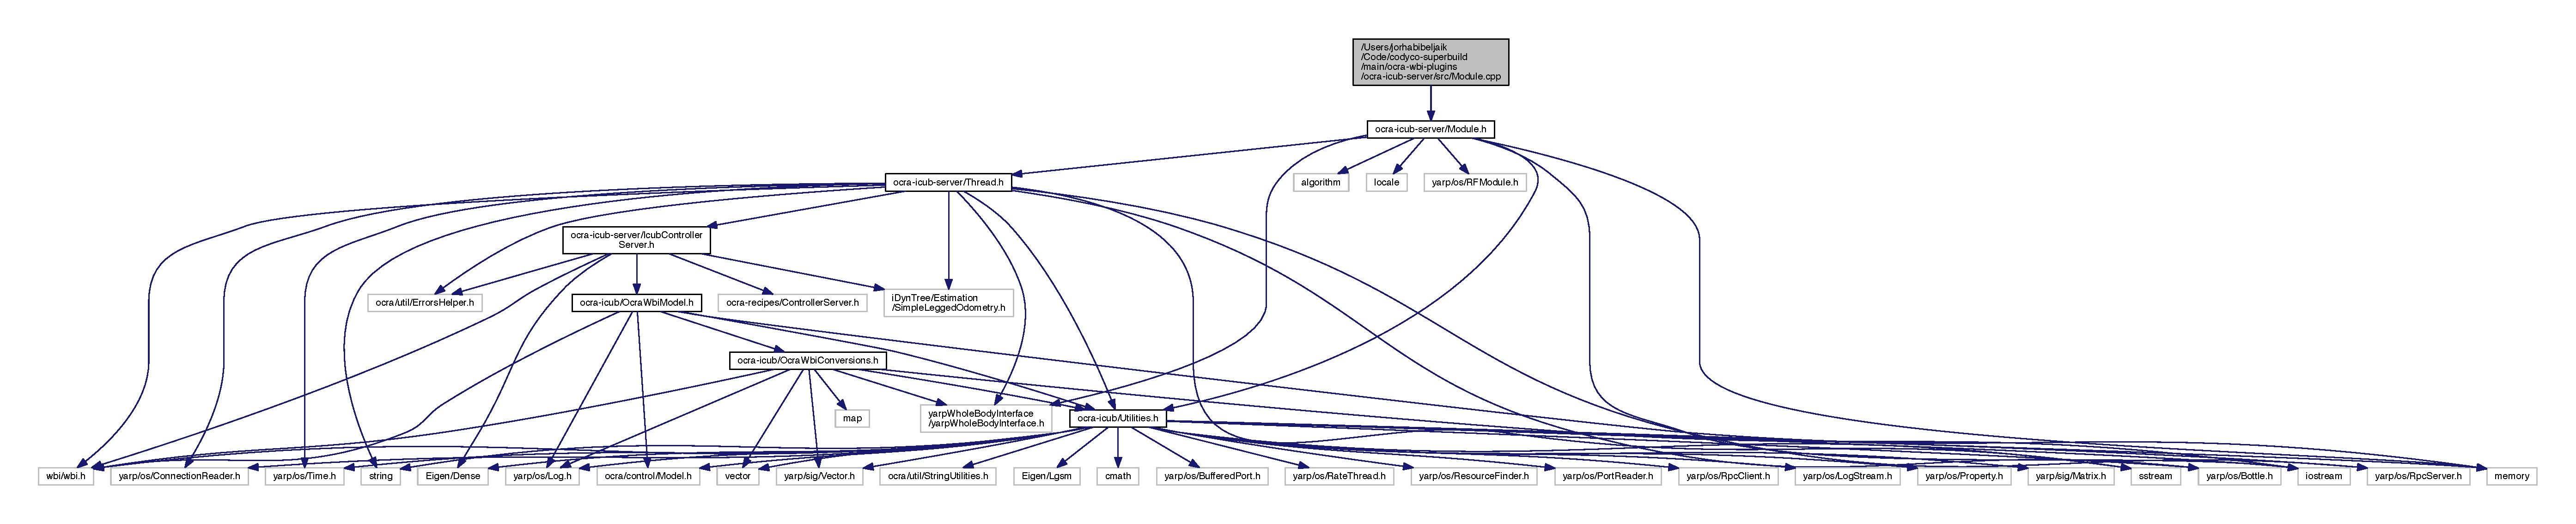
\includegraphics[width=350pt]{Module_8cpp__incl}
\end{center}
\end{figure}

\hypertarget{Thread_8cpp}{}\section{/\+Users/jorhabibeljaik/\+Code/codyco-\/superbuild/main/ocra-\/wbi-\/plugins/ocra-\/icub-\/server/src/\+Thread.cpp File Reference}
\label{Thread_8cpp}\index{/\+Users/jorhabibeljaik/\+Code/codyco-\/superbuild/main/ocra-\/wbi-\/plugins/ocra-\/icub-\/server/src/\+Thread.\+cpp@{/\+Users/jorhabibeljaik/\+Code/codyco-\/superbuild/main/ocra-\/wbi-\/plugins/ocra-\/icub-\/server/src/\+Thread.\+cpp}}


The thread class for the controller server.  


{\ttfamily \#include \char`\"{}ocra-\/icub-\/server/\+Thread.\+h\char`\"{}}\newline
\subsection*{Functions}
\begin{DoxyCompactItemize}
\item 
std\+::ostream \& \hyperlink{Thread_8cpp_a30ab3a18ec4f8101aa6f1df6926888f6}{operator$<$$<$} (std\+::ostream \&out, const \hyperlink{classOcraControllerOptions}{Ocra\+Controller\+Options} \&opts)
\end{DoxyCompactItemize}


\subsection{Detailed Description}
The thread class for the controller server. 

\begin{DoxyAuthor}{Author}
\href{http://www.ryanlober.com}{\tt Ryan Lober} 

\href{http://ahoarau.github.io}{\tt Antoine Hoarau} 
\end{DoxyAuthor}
\begin{DoxyDate}{Date}
Feb 2016 
\end{DoxyDate}
\begin{DoxyCopyright}{Copyright}
G\+NU General Public License. 
\end{DoxyCopyright}


\subsection{Function Documentation}
\hypertarget{Thread_8cpp_a30ab3a18ec4f8101aa6f1df6926888f6}{}\label{Thread_8cpp_a30ab3a18ec4f8101aa6f1df6926888f6} 
\index{Thread.\+cpp@{Thread.\+cpp}!operator$<$$<$@{operator$<$$<$}}
\index{operator$<$$<$@{operator$<$$<$}!Thread.\+cpp@{Thread.\+cpp}}
\subsubsection{\texorpdfstring{operator$<$$<$()}{operator<<()}}
{\footnotesize\ttfamily std\+::ostream\& operator$<$$<$ (\begin{DoxyParamCaption}\item[{std\+::ostream \&}]{out,  }\item[{const \hyperlink{classOcraControllerOptions}{Ocra\+Controller\+Options} \&}]{opts }\end{DoxyParamCaption})}


\hypertarget{IcubClient_8h}{}\section{/\+Users/jorhabibeljaik/\+Code/codyco-\/superbuild/main/ocra-\/wbi-\/plugins/ocra-\/icub/include/ocra-\/icub/\+Icub\+Client.h File Reference}
\label{IcubClient_8h}\index{/\+Users/jorhabibeljaik/\+Code/codyco-\/superbuild/main/ocra-\/wbi-\/plugins/ocra-\/icub/include/ocra-\/icub/\+Icub\+Client.\+h@{/\+Users/jorhabibeljaik/\+Code/codyco-\/superbuild/main/ocra-\/wbi-\/plugins/ocra-\/icub/include/ocra-\/icub/\+Icub\+Client.\+h}}
{\ttfamily \#include $<$ocra-\/icub/\+Model\+Initializer.\+h$>$}\newline
{\ttfamily \#include $<$ocra-\/icub/\+Ocra\+Wbi\+Conversions.\+h$>$}\newline
{\ttfamily \#include $<$ocra-\/icub/\+Ocra\+Wbi\+Model.\+h$>$}\newline
{\ttfamily \#include $<$ocra-\/icub/\+Utilities.\+h$>$}\newline
Include dependency graph for Icub\+Client.\+h\+:\nopagebreak
\begin{figure}[H]
\begin{center}
\leavevmode
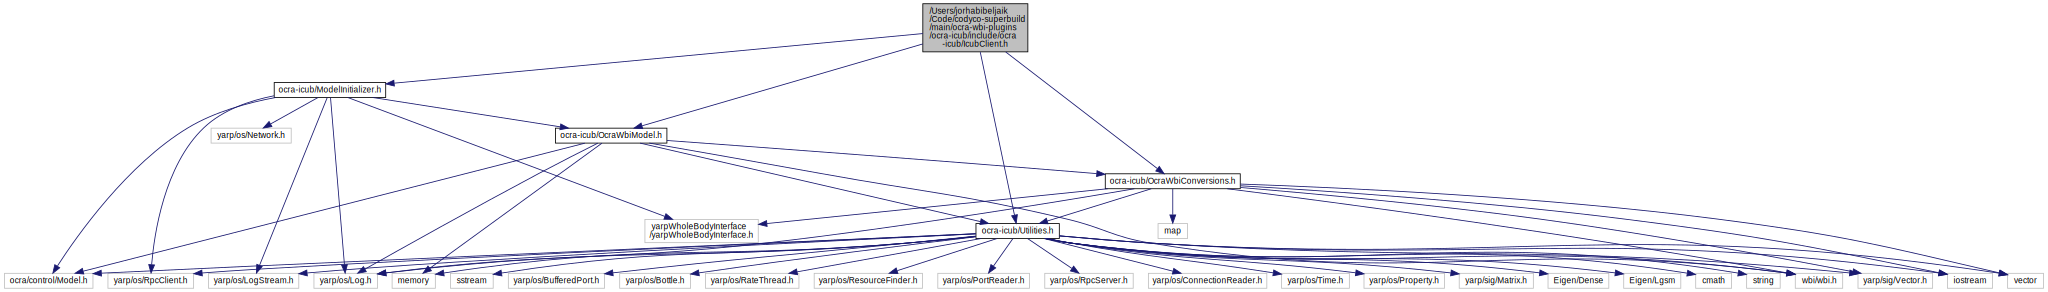
\includegraphics[width=350pt]{IcubClient_8h__incl}
\end{center}
\end{figure}
This graph shows which files directly or indirectly include this file\+:\nopagebreak
\begin{figure}[H]
\begin{center}
\leavevmode
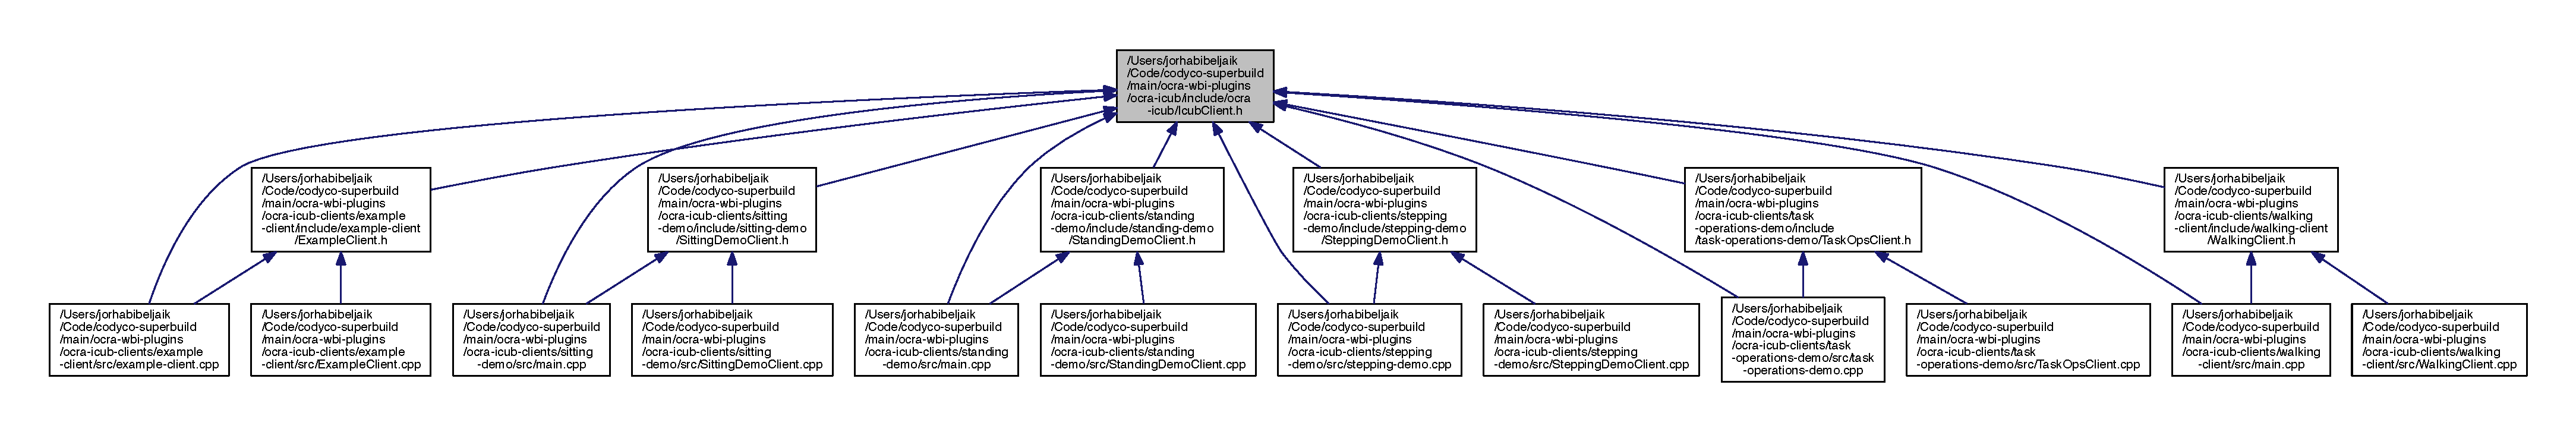
\includegraphics[width=350pt]{IcubClient_8h__dep__incl}
\end{center}
\end{figure}

\hypertarget{ModelInitializer_8h}{}\section{/\+Users/jorhabibeljaik/\+Code/codyco-\/superbuild/main/ocra-\/wbi-\/plugins/ocra-\/icub/include/ocra-\/icub/\+Model\+Initializer.h File Reference}
\label{ModelInitializer_8h}\index{/\+Users/jorhabibeljaik/\+Code/codyco-\/superbuild/main/ocra-\/wbi-\/plugins/ocra-\/icub/include/ocra-\/icub/\+Model\+Initializer.\+h@{/\+Users/jorhabibeljaik/\+Code/codyco-\/superbuild/main/ocra-\/wbi-\/plugins/ocra-\/icub/include/ocra-\/icub/\+Model\+Initializer.\+h}}
{\ttfamily \#include $<$ocra-\/icub/\+Ocra\+Wbi\+Model.\+h$>$}\newline
{\ttfamily \#include $<$ocra/control/\+Model.\+h$>$}\newline
{\ttfamily \#include $<$yarp\+Whole\+Body\+Interface/yarp\+Whole\+Body\+Interface.\+h$>$}\newline
{\ttfamily \#include $<$yarp/os/\+Rpc\+Client.\+h$>$}\newline
{\ttfamily \#include $<$yarp/os/\+Network.\+h$>$}\newline
{\ttfamily \#include $<$yarp/os/\+Log\+Stream.\+h$>$}\newline
{\ttfamily \#include $<$yarp/os/\+Log.\+h$>$}\newline
Include dependency graph for Model\+Initializer.\+h\+:
\nopagebreak
\begin{figure}[H]
\begin{center}
\leavevmode
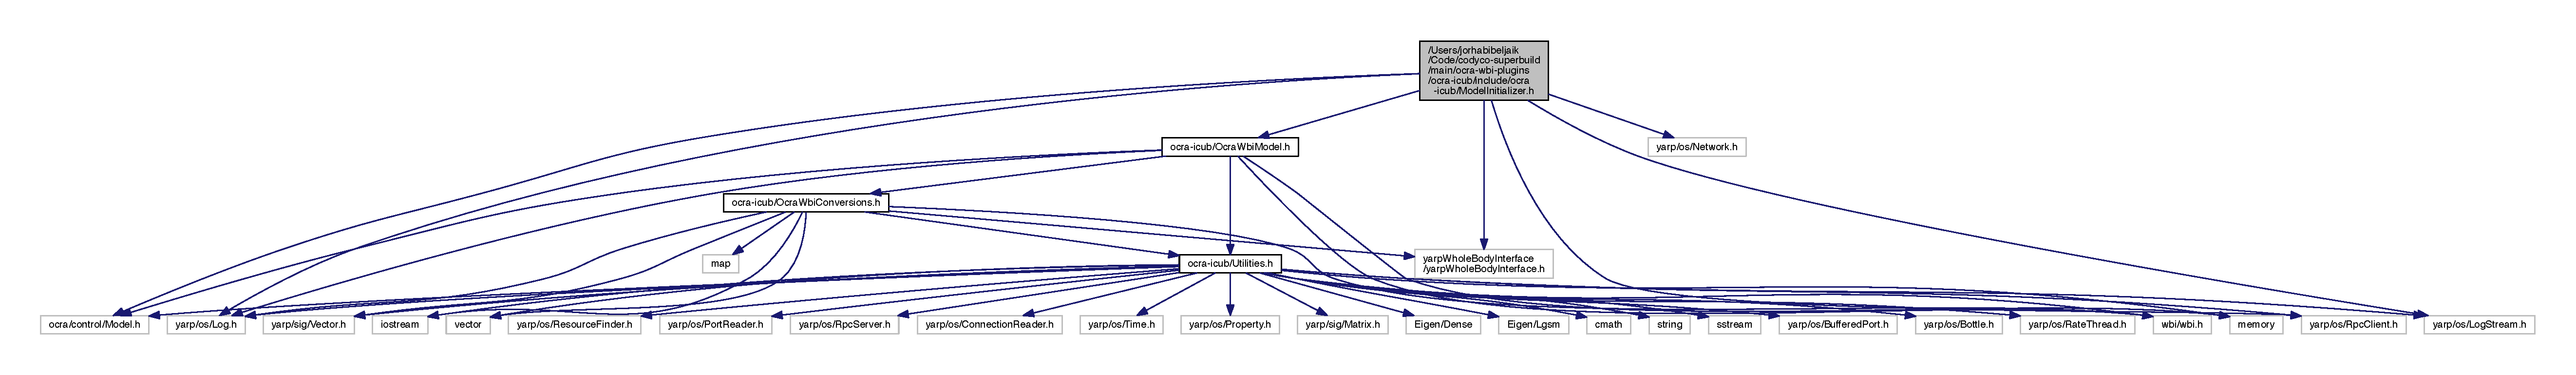
\includegraphics[width=350pt]{ModelInitializer_8h__incl}
\end{center}
\end{figure}
This graph shows which files directly or indirectly include this file\+:
\nopagebreak
\begin{figure}[H]
\begin{center}
\leavevmode
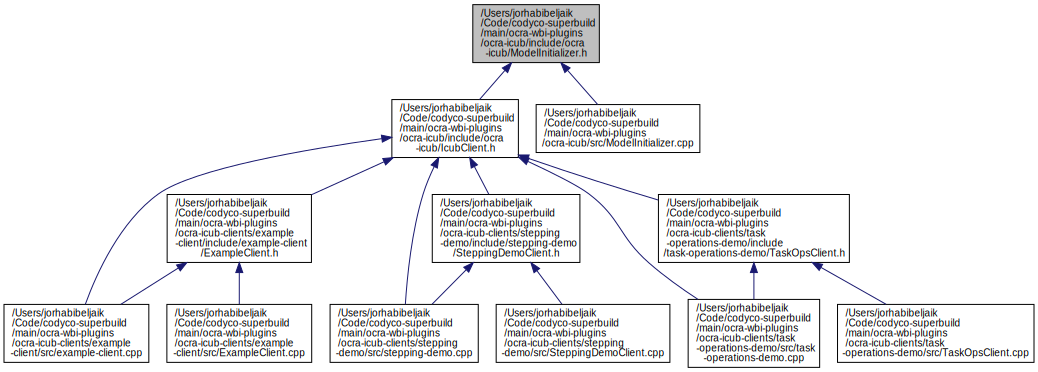
\includegraphics[width=350pt]{ModelInitializer_8h__dep__incl}
\end{center}
\end{figure}
\subsection*{Classes}
\begin{DoxyCompactItemize}
\item 
class \hyperlink{classocra__icub_1_1ModelInitializer}{ocra\+\_\+icub\+::\+Model\+Initializer}
\end{DoxyCompactItemize}
\subsection*{Namespaces}
\begin{DoxyCompactItemize}
\item 
 \hyperlink{namespaceocra__icub}{ocra\+\_\+icub}
\end{DoxyCompactItemize}

\hypertarget{OcraWbiConversions_8h}{}\section{/\+Users/jorhabibeljaik/\+Code/codyco-\/superbuild/main/ocra-\/wbi-\/plugins/ocra-\/icub/include/ocra-\/icub/\+Ocra\+Wbi\+Conversions.h File Reference}
\label{OcraWbiConversions_8h}\index{/\+Users/jorhabibeljaik/\+Code/codyco-\/superbuild/main/ocra-\/wbi-\/plugins/ocra-\/icub/include/ocra-\/icub/\+Ocra\+Wbi\+Conversions.\+h@{/\+Users/jorhabibeljaik/\+Code/codyco-\/superbuild/main/ocra-\/wbi-\/plugins/ocra-\/icub/include/ocra-\/icub/\+Ocra\+Wbi\+Conversions.\+h}}


A utility class full of static conversion functions.  


{\ttfamily \#include $<$iostream$>$}\newline
{\ttfamily \#include $<$map$>$}\newline
{\ttfamily \#include $<$vector$>$}\newline
{\ttfamily \#include $<$yarp/sig/\+Vector.\+h$>$}\newline
{\ttfamily \#include $<$yarp/os/\+Log.\+h$>$}\newline
{\ttfamily \#include $<$wbi/wbi.\+h$>$}\newline
{\ttfamily \#include $<$yarp\+Whole\+Body\+Interface/yarp\+Whole\+Body\+Interface.\+h$>$}\newline
{\ttfamily \#include \char`\"{}ocra-\/icub/\+Utilities.\+h\char`\"{}}\newline
Include dependency graph for Ocra\+Wbi\+Conversions.\+h\+:\nopagebreak
\begin{figure}[H]
\begin{center}
\leavevmode
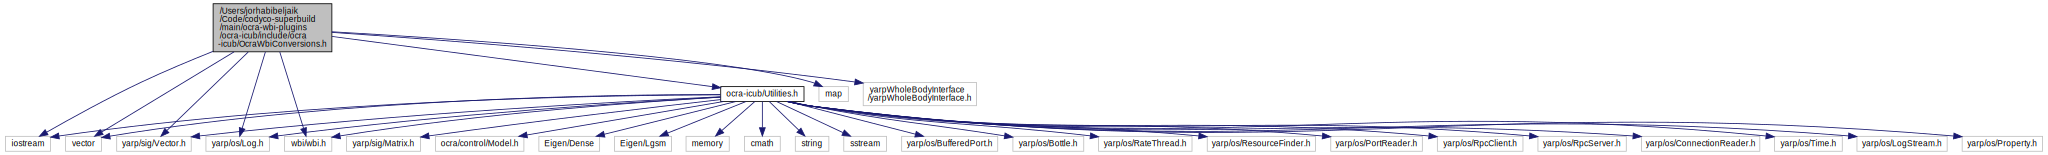
\includegraphics[width=350pt]{OcraWbiConversions_8h__incl}
\end{center}
\end{figure}
This graph shows which files directly or indirectly include this file\+:\nopagebreak
\begin{figure}[H]
\begin{center}
\leavevmode
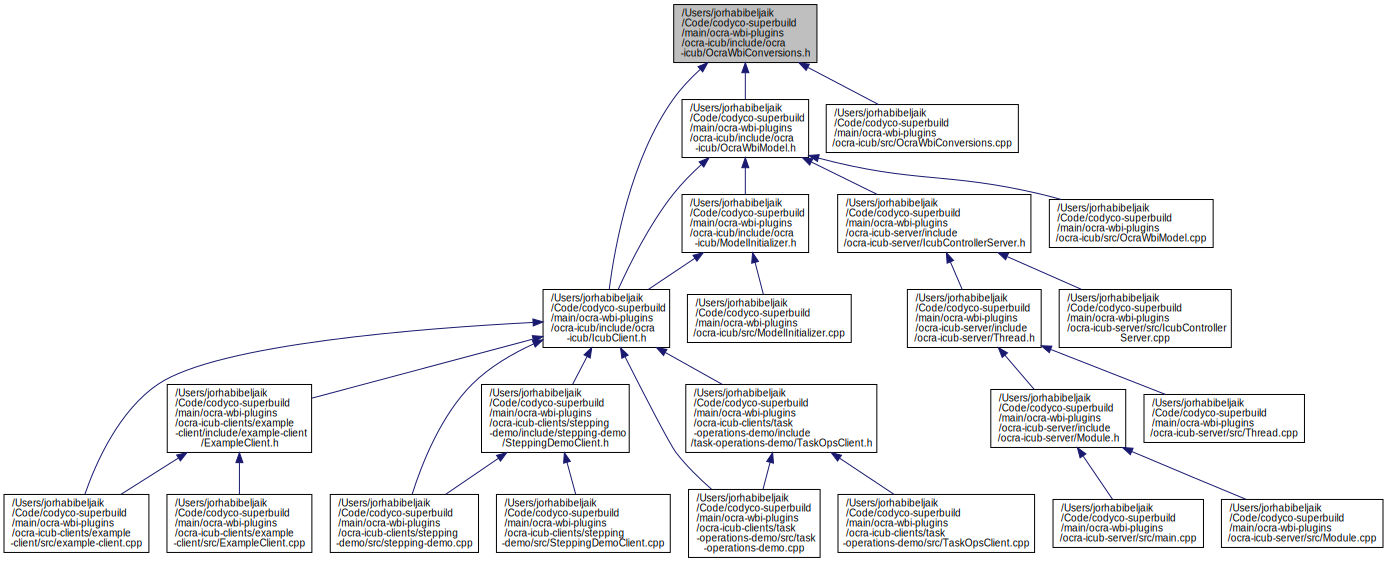
\includegraphics[width=350pt]{OcraWbiConversions_8h__dep__incl}
\end{center}
\end{figure}
\subsection*{Classes}
\begin{DoxyCompactItemize}
\item 
class \hyperlink{classocra__icub_1_1OcraWbiConversions}{ocra\+\_\+icub\+::\+Ocra\+Wbi\+Conversions}
\end{DoxyCompactItemize}
\subsection*{Namespaces}
\begin{DoxyCompactItemize}
\item 
 \hyperlink{namespaceocra__icub}{ocra\+\_\+icub}
\end{DoxyCompactItemize}
\subsection*{Typedefs}
\begin{DoxyCompactItemize}
\item 
typedef Eigen\+::\+Matrix$<$ double, Eigen\+::\+Dynamic, Eigen\+::\+Dynamic, Eigen\+::\+Row\+Major $>$ \hyperlink{namespaceocra__icub_aa5e36a19ed031c28ca83c207bd7dd83f}{ocra\+\_\+icub\+::\+Matrix\+Xd\+Rm}
\end{DoxyCompactItemize}


\subsection{Detailed Description}
A utility class full of static conversion functions. 

\begin{DoxyAuthor}{Author}
\href{http://www.ryanlober.com}{\tt Ryan Lober} 

\href{http://ahoarau.github.io}{\tt Antoine Hoarau} 
\end{DoxyAuthor}
\begin{DoxyDate}{Date}
Feb 2016 
\end{DoxyDate}
\begin{DoxyCopyright}{Copyright}
G\+NU General Public License. 
\end{DoxyCopyright}

\hypertarget{OcraWbiModel_8h}{}\section{/\+Users/jorhabibeljaik/\+Code/codyco-\/superbuild/main/ocra-\/wbi-\/plugins/ocra-\/icub/include/ocra-\/icub/\+Ocra\+Wbi\+Model.h File Reference}
\label{OcraWbiModel_8h}\index{/\+Users/jorhabibeljaik/\+Code/codyco-\/superbuild/main/ocra-\/wbi-\/plugins/ocra-\/icub/include/ocra-\/icub/\+Ocra\+Wbi\+Model.\+h@{/\+Users/jorhabibeljaik/\+Code/codyco-\/superbuild/main/ocra-\/wbi-\/plugins/ocra-\/icub/include/ocra-\/icub/\+Ocra\+Wbi\+Model.\+h}}


Implementation of ocra\+::\+Model using whole\+Body\+Interface.  


{\ttfamily \#include $<$memory$>$}\newline
{\ttfamily \#include \char`\"{}ocra/control/\+Model.\+h\char`\"{}}\newline
{\ttfamily \#include $<$wbi/wbi.\+h$>$}\newline
{\ttfamily \#include $<$yarp/os/\+Log.\+h$>$}\newline
{\ttfamily \#include \char`\"{}ocra-\/icub/\+Ocra\+Wbi\+Conversions.\+h\char`\"{}}\newline
{\ttfamily \#include \char`\"{}ocra-\/icub/\+Utilities.\+h\char`\"{}}\newline
Include dependency graph for Ocra\+Wbi\+Model.\+h\+:
\nopagebreak
\begin{figure}[H]
\begin{center}
\leavevmode
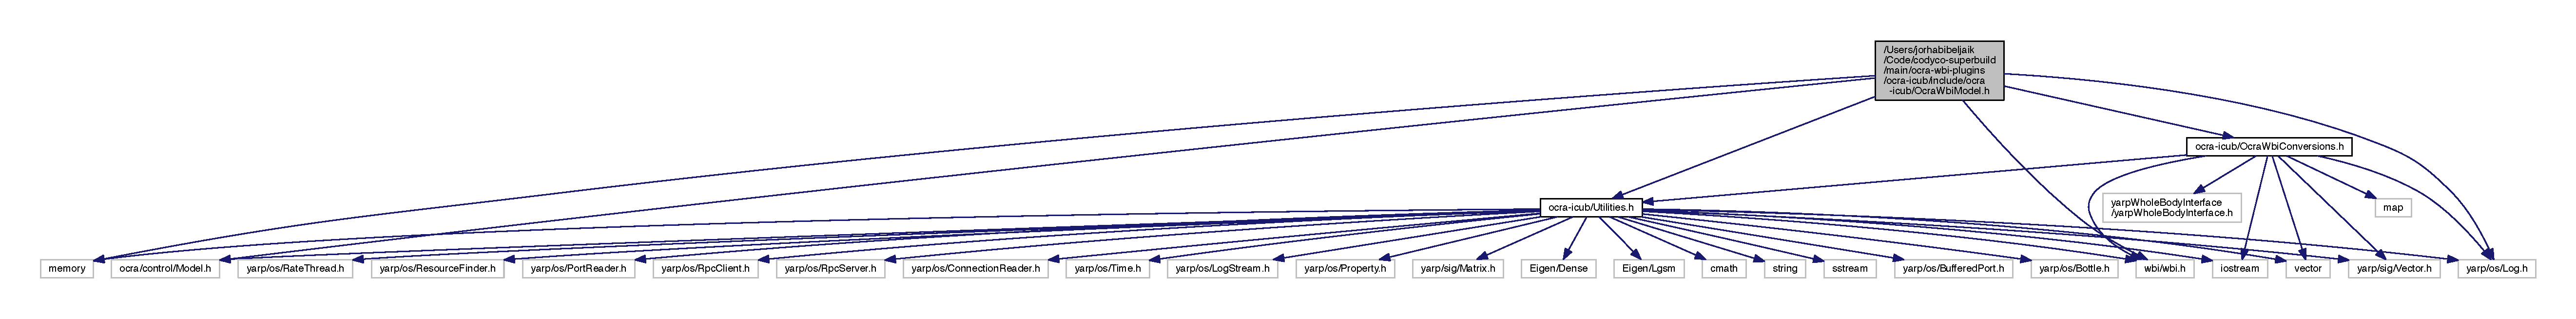
\includegraphics[width=350pt]{OcraWbiModel_8h__incl}
\end{center}
\end{figure}
This graph shows which files directly or indirectly include this file\+:
\nopagebreak
\begin{figure}[H]
\begin{center}
\leavevmode
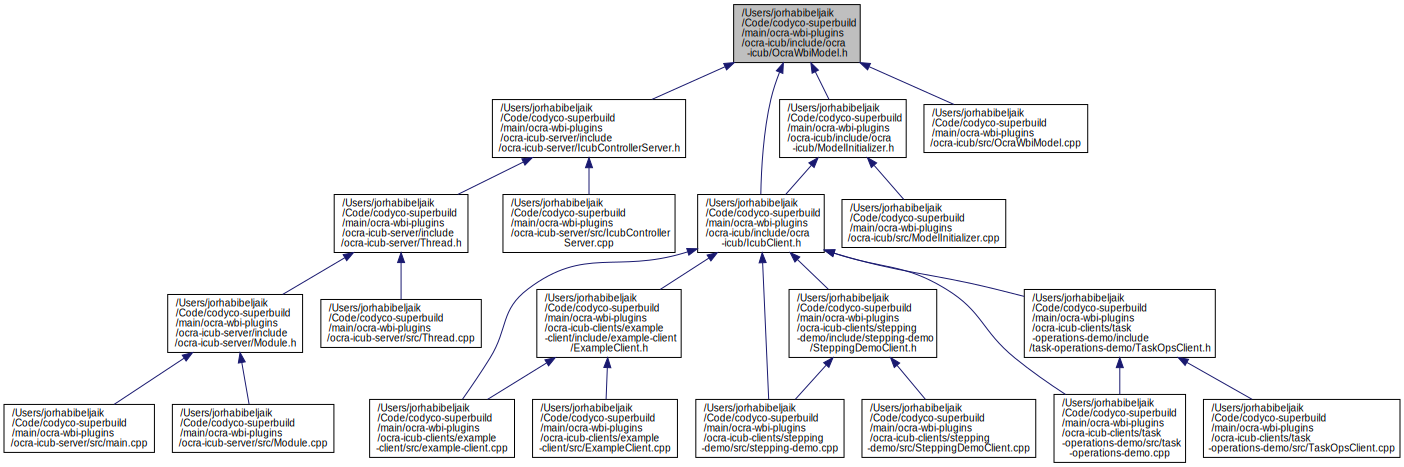
\includegraphics[width=350pt]{OcraWbiModel_8h__dep__incl}
\end{center}
\end{figure}
\subsection*{Classes}
\begin{DoxyCompactItemize}
\item 
class \hyperlink{classocra__icub_1_1OcraWbiModel}{ocra\+\_\+icub\+::\+Ocra\+Wbi\+Model}
\end{DoxyCompactItemize}
\subsection*{Namespaces}
\begin{DoxyCompactItemize}
\item 
 \hyperlink{namespaceocra__icub}{ocra\+\_\+icub}
\end{DoxyCompactItemize}


\subsection{Detailed Description}
Implementation of ocra\+::\+Model using whole\+Body\+Interface. 

\begin{DoxyAuthor}{Author}
\href{http://www.ryanlober.com}{\tt Ryan Lober} 

\href{http://ahoarau.github.io}{\tt Antoine Hoarau} 
\end{DoxyAuthor}
\begin{DoxyDate}{Date}
Feb 2016 
\end{DoxyDate}
\begin{DoxyCopyright}{Copyright}
G\+NU General Public License. 
\end{DoxyCopyright}

\hypertarget{Utilities_8h}{}\section{/\+Users/jorhabibeljaik/\+Code/codyco-\/superbuild/main/ocra-\/wbi-\/plugins/ocra-\/icub/include/ocra-\/icub/\+Utilities.h File Reference}
\label{Utilities_8h}\index{/\+Users/jorhabibeljaik/\+Code/codyco-\/superbuild/main/ocra-\/wbi-\/plugins/ocra-\/icub/include/ocra-\/icub/\+Utilities.\+h@{/\+Users/jorhabibeljaik/\+Code/codyco-\/superbuild/main/ocra-\/wbi-\/plugins/ocra-\/icub/include/ocra-\/icub/\+Utilities.\+h}}


Some useful tools for the ocra-\/icub lib.  


{\ttfamily \#include $<$memory$>$}\newline
{\ttfamily \#include $<$cmath$>$}\newline
{\ttfamily \#include $<$iostream$>$}\newline
{\ttfamily \#include $<$string$>$}\newline
{\ttfamily \#include $<$vector$>$}\newline
{\ttfamily \#include $<$sstream$>$}\newline
{\ttfamily \#include $<$yarp/os/\+Buffered\+Port.\+h$>$}\newline
{\ttfamily \#include $<$yarp/os/\+Bottle.\+h$>$}\newline
{\ttfamily \#include $<$yarp/os/\+Rate\+Thread.\+h$>$}\newline
{\ttfamily \#include $<$yarp/os/\+Resource\+Finder.\+h$>$}\newline
{\ttfamily \#include $<$yarp/os/\+Port\+Reader.\+h$>$}\newline
{\ttfamily \#include $<$yarp/os/\+Rpc\+Client.\+h$>$}\newline
{\ttfamily \#include $<$yarp/os/\+Rpc\+Server.\+h$>$}\newline
{\ttfamily \#include $<$yarp/os/\+Connection\+Reader.\+h$>$}\newline
{\ttfamily \#include $<$yarp/os/\+Time.\+h$>$}\newline
{\ttfamily \#include $<$yarp/os/\+Log.\+h$>$}\newline
{\ttfamily \#include $<$yarp/os/\+Log\+Stream.\+h$>$}\newline
{\ttfamily \#include $<$yarp/os/\+Property.\+h$>$}\newline
{\ttfamily \#include $<$yarp/sig/\+Vector.\+h$>$}\newline
{\ttfamily \#include $<$yarp/sig/\+Matrix.\+h$>$}\newline
{\ttfamily \#include $<$wbi/wbi.\+h$>$}\newline
{\ttfamily \#include \char`\"{}ocra/control/\+Model.\+h\char`\"{}}\newline
{\ttfamily \#include $<$Eigen/\+Dense$>$}\newline
{\ttfamily \#include $<$Eigen/\+Lgsm$>$}\newline
Include dependency graph for Utilities.\+h\+:\nopagebreak
\begin{figure}[H]
\begin{center}
\leavevmode
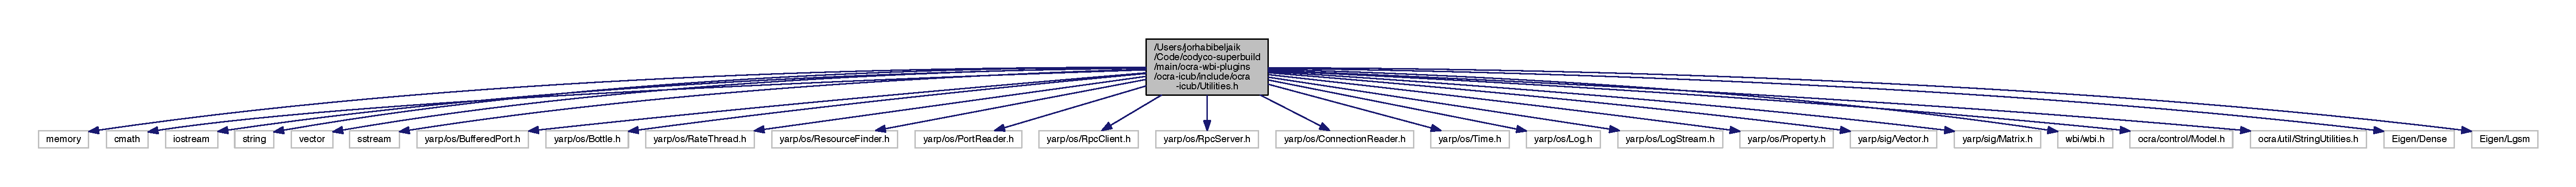
\includegraphics[width=350pt]{Utilities_8h__incl}
\end{center}
\end{figure}
This graph shows which files directly or indirectly include this file\+:
\nopagebreak
\begin{figure}[H]
\begin{center}
\leavevmode
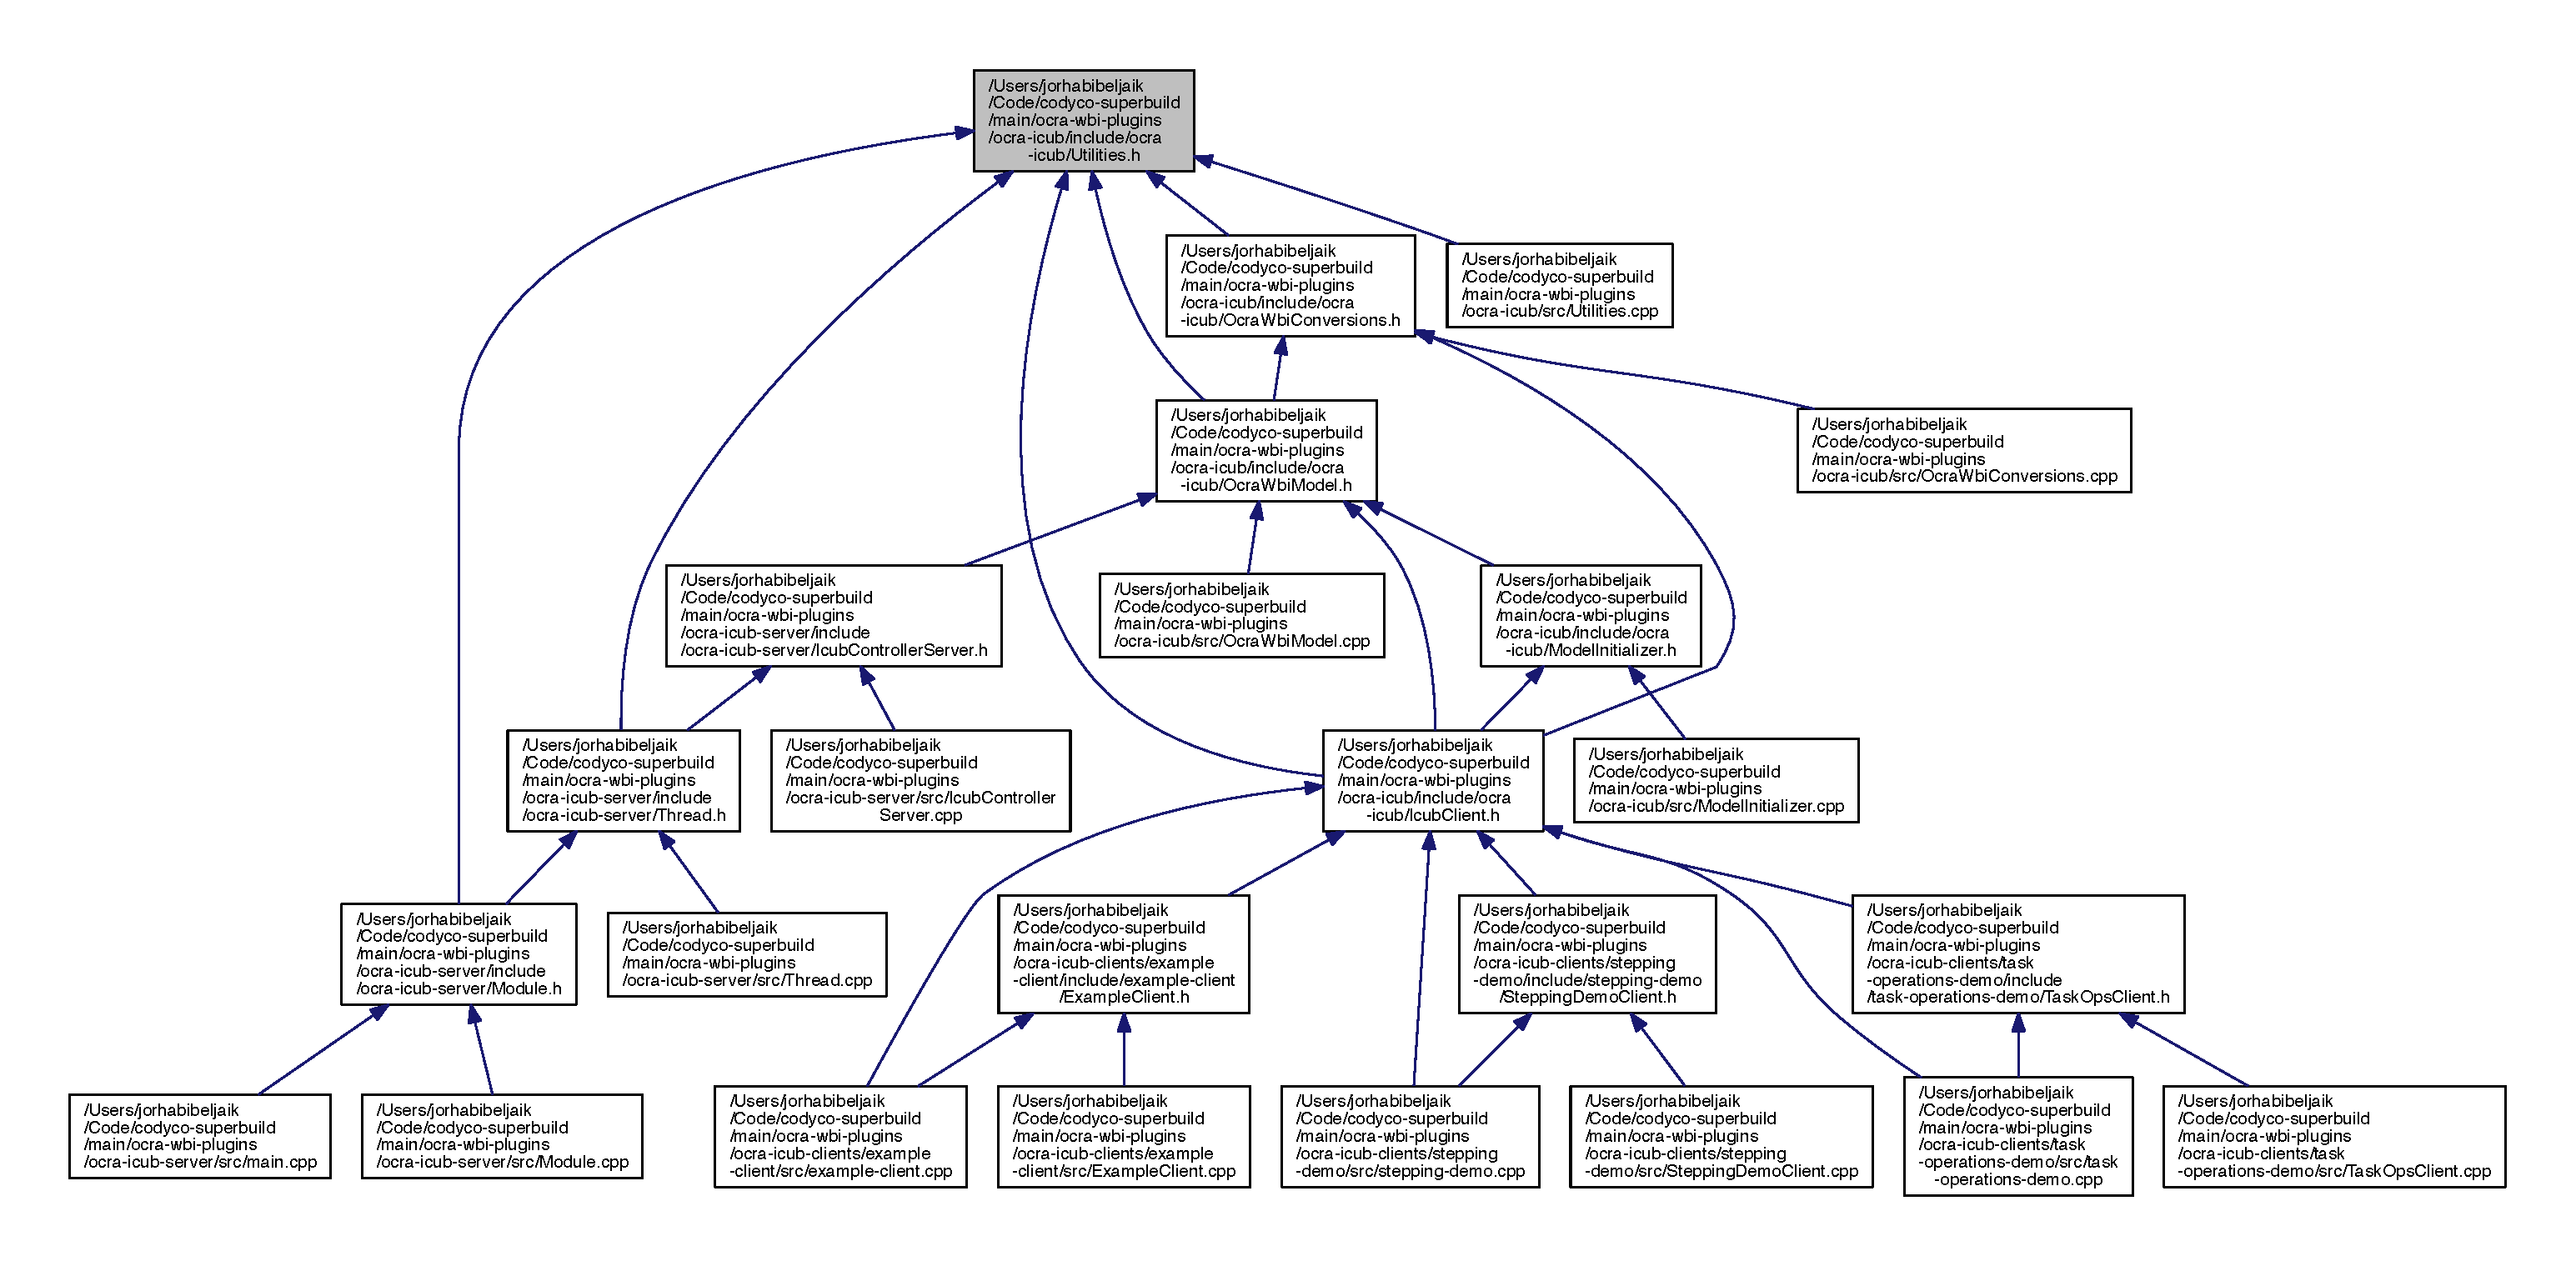
\includegraphics[width=350pt]{Utilities_8h__dep__incl}
\end{center}
\end{figure}
\subsection*{Namespaces}
\begin{DoxyCompactItemize}
\item 
 \hyperlink{namespaceocra__icub}{ocra\+\_\+icub}
\end{DoxyCompactItemize}
\subsection*{Macros}
\begin{DoxyCompactItemize}
\item 
\#define \hyperlink{Utilities_8h_a986e6d54948ebf3007dc52bd0fc737be}{C\+L\+A\+S\+S\+\_\+\+P\+O\+I\+N\+T\+E\+R\+\_\+\+T\+Y\+P\+E\+D\+E\+FS}(Class)
\end{DoxyCompactItemize}
\subsection*{Enumerations}
\begin{DoxyCompactItemize}
\item 
enum \hyperlink{namespaceocra__icub_afbd2db66b68005fb7cfac19210caf83f}{ocra\+\_\+icub\+::\+O\+C\+R\+A\+\_\+\+I\+C\+U\+B\+\_\+\+M\+E\+S\+S\+A\+GE} \{ \newline
\hyperlink{namespaceocra__icub_afbd2db66b68005fb7cfac19210caf83faa0c1832978fad84ef108d48265af68d2}{ocra\+\_\+icub\+::\+F\+A\+I\+L\+U\+RE} = 0, 
\hyperlink{namespaceocra__icub_afbd2db66b68005fb7cfac19210caf83fa67c96e3afcb39533f69c97dc5e9734e5}{ocra\+\_\+icub\+::\+S\+U\+C\+C\+E\+SS}, 
\hyperlink{namespaceocra__icub_afbd2db66b68005fb7cfac19210caf83fae8fe02f5f3b1b11d4749e720b9ec3636}{ocra\+\_\+icub\+::\+G\+E\+T\+\_\+\+M\+O\+D\+E\+L\+\_\+\+C\+O\+N\+F\+I\+G\+\_\+\+I\+N\+FO}, 
\hyperlink{namespaceocra__icub_afbd2db66b68005fb7cfac19210caf83fa772ab917d1ff28db029af9271208a69a}{ocra\+\_\+icub\+::\+G\+E\+T\+\_\+\+C\+O\+N\+T\+R\+O\+L\+L\+E\+R\+\_\+\+S\+E\+R\+V\+E\+R\+\_\+\+S\+T\+A\+T\+US}, 
\newline
\hyperlink{namespaceocra__icub_afbd2db66b68005fb7cfac19210caf83fa5dee3cfa0ab6c29f5546bc9e30c0aef5}{ocra\+\_\+icub\+::\+C\+O\+N\+T\+R\+O\+L\+L\+E\+R\+\_\+\+S\+E\+R\+V\+E\+R\+\_\+\+R\+U\+N\+N\+I\+NG}, 
\hyperlink{namespaceocra__icub_afbd2db66b68005fb7cfac19210caf83fafd31e40d18e553fc09105d360455bc49}{ocra\+\_\+icub\+::\+C\+O\+N\+T\+R\+O\+L\+L\+E\+R\+\_\+\+S\+E\+R\+V\+E\+R\+\_\+\+S\+T\+O\+P\+P\+ED}, 
\hyperlink{namespaceocra__icub_afbd2db66b68005fb7cfac19210caf83fa48ad7962d035a58257a0381872ce27b1}{ocra\+\_\+icub\+::\+C\+O\+N\+T\+R\+O\+L\+L\+E\+R\+\_\+\+S\+E\+R\+V\+E\+R\+\_\+\+P\+A\+U\+S\+ED}, 
\hyperlink{namespaceocra__icub_afbd2db66b68005fb7cfac19210caf83fae7c9fa2563b6c0b14e5b05d1794dac36}{ocra\+\_\+icub\+::\+H\+E\+LP}
 \}
\end{DoxyCompactItemize}
\subsection*{Functions}
\begin{DoxyCompactItemize}
\item 
void \hyperlink{namespaceocra__icub_a07ffe33877389b6b111944e8a666e221}{ocra\+\_\+icub\+::get\+Nominal\+Posture} (const ocra\+::\+Model \&model, Eigen\+::\+Vector\+Xd \&q)
\item 
void \hyperlink{namespaceocra__icub_a91c3caf94014ea9988e56dd2572768ce}{ocra\+\_\+icub\+::get\+Home\+Posture} (const ocra\+::\+Model \&model, Eigen\+::\+Vector\+Xd \&q)
\end{DoxyCompactItemize}
\subsection*{Variables}
\begin{DoxyCompactItemize}
\item 
static constexpr double \hyperlink{namespaceocra__icub_ab06477ded34ed5514b911a3511b22e3d}{ocra\+\_\+icub\+::\+D\+E\+G\+\_\+\+T\+O\+\_\+\+R\+AD} = M\+\_\+\+PI/180.\+0
\end{DoxyCompactItemize}


\subsection{Detailed Description}
Some useful tools for the ocra-\/icub lib. 

This file is for all the various macros and helper classes that are generic to ocra-\/icub. It is also a place for all the repeated includes like standard stl includes etc. \begin{DoxyAuthor}{Author}
\href{http://www.ryanlober.com}{\tt Ryan Lober} 
\end{DoxyAuthor}
\begin{DoxyDate}{Date}
Feb 2016 
\end{DoxyDate}
\begin{DoxyCopyright}{Copyright}
G\+NU General Public License. 
\end{DoxyCopyright}


\subsection{Macro Definition Documentation}
\hypertarget{Utilities_8h_a986e6d54948ebf3007dc52bd0fc737be}{}\label{Utilities_8h_a986e6d54948ebf3007dc52bd0fc737be} 
\index{Utilities.\+h@{Utilities.\+h}!C\+L\+A\+S\+S\+\_\+\+P\+O\+I\+N\+T\+E\+R\+\_\+\+T\+Y\+P\+E\+D\+E\+FS@{C\+L\+A\+S\+S\+\_\+\+P\+O\+I\+N\+T\+E\+R\+\_\+\+T\+Y\+P\+E\+D\+E\+FS}}
\index{C\+L\+A\+S\+S\+\_\+\+P\+O\+I\+N\+T\+E\+R\+\_\+\+T\+Y\+P\+E\+D\+E\+FS@{C\+L\+A\+S\+S\+\_\+\+P\+O\+I\+N\+T\+E\+R\+\_\+\+T\+Y\+P\+E\+D\+E\+FS}!Utilities.\+h@{Utilities.\+h}}
\subsubsection{\texorpdfstring{C\+L\+A\+S\+S\+\_\+\+P\+O\+I\+N\+T\+E\+R\+\_\+\+T\+Y\+P\+E\+D\+E\+FS}{CLASS\_POINTER\_TYPEDEFS}}
{\footnotesize\ttfamily \#define C\+L\+A\+S\+S\+\_\+\+P\+O\+I\+N\+T\+E\+R\+\_\+\+T\+Y\+P\+E\+D\+E\+FS(\begin{DoxyParamCaption}\item[{}]{Class }\end{DoxyParamCaption})}

{\bfseries Value\+:}
\begin{DoxyCode}
\textcolor{keyword}{public}:\(\backslash\)
using ptr           = std::shared\_ptr   <Class>;  \(\backslash\)
using shared\_ptr    = std::shared\_ptr   <Class>;  \(\backslash\)
using unique\_ptr    = std::unique\_ptr   <Class>;  \(\backslash\)
using weak\_ptr      = std::weak\_ptr     <Class>;  \(\backslash\)
using const\_ptr           = \textcolor{keyword}{const} std::shared\_ptr   <Class>;  \(\backslash\)
using const\_shared\_ptr    = \textcolor{keyword}{const} std::shared\_ptr   <Class>;  \(\backslash\)
using const\_unique\_ptr    = \textcolor{keyword}{const} std::unique\_ptr   <Class>;  \(\backslash\)
using const\_weak\_ptr      = \textcolor{keyword}{const} std::weak\_ptr     <Class>;
\end{DoxyCode}
Macro function which basically just defines pointer typdefs for classes. Note that normally macros are evil monsters but I think this is a perfect usage case to cut down on repeated code. 
\begin{DoxyParams}{Parameters}
{\em Class} & Just pop this bad boy below the class definition and it will do the rest. \\
\hline
\end{DoxyParams}

\hypertarget{ModelInitializer_8cpp}{}\section{/\+Users/jorhabibeljaik/\+Code/codyco-\/superbuild/main/ocra-\/wbi-\/plugins/ocra-\/icub/src/\+Model\+Initializer.cpp File Reference}
\label{ModelInitializer_8cpp}\index{/\+Users/jorhabibeljaik/\+Code/codyco-\/superbuild/main/ocra-\/wbi-\/plugins/ocra-\/icub/src/\+Model\+Initializer.\+cpp@{/\+Users/jorhabibeljaik/\+Code/codyco-\/superbuild/main/ocra-\/wbi-\/plugins/ocra-\/icub/src/\+Model\+Initializer.\+cpp}}
{\ttfamily \#include $<$ocra-\/icub/\+Model\+Initializer.\+h$>$}\newline

\hypertarget{OcraWbiConversions_8cpp}{}\section{/\+Users/jorhabibeljaik/\+Code/codyco-\/superbuild/main/ocra-\/wbi-\/plugins/ocra-\/icub/src/\+Ocra\+Wbi\+Conversions.cpp File Reference}
\label{OcraWbiConversions_8cpp}\index{/\+Users/jorhabibeljaik/\+Code/codyco-\/superbuild/main/ocra-\/wbi-\/plugins/ocra-\/icub/src/\+Ocra\+Wbi\+Conversions.\+cpp@{/\+Users/jorhabibeljaik/\+Code/codyco-\/superbuild/main/ocra-\/wbi-\/plugins/ocra-\/icub/src/\+Ocra\+Wbi\+Conversions.\+cpp}}


A utility class full of static conversion functions.  


{\ttfamily \#include $<$ocra-\/icub/\+Ocra\+Wbi\+Conversions.\+h$>$}\newline
Include dependency graph for Ocra\+Wbi\+Conversions.\+cpp\+:
\nopagebreak
\begin{figure}[H]
\begin{center}
\leavevmode
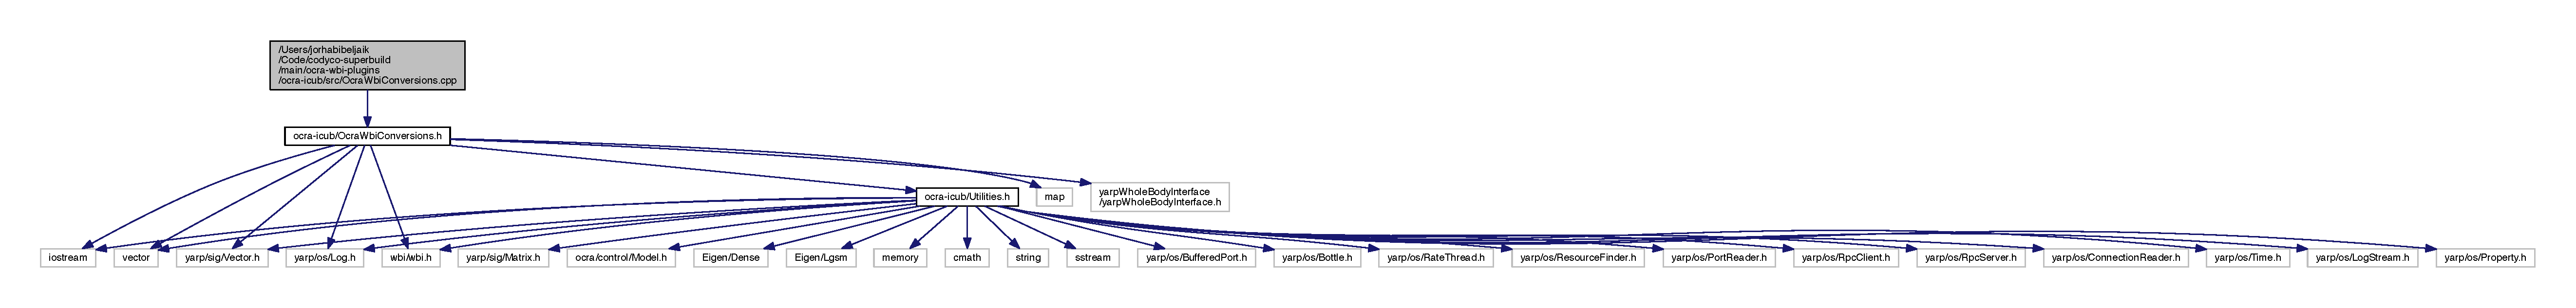
\includegraphics[width=350pt]{OcraWbiConversions_8cpp__incl}
\end{center}
\end{figure}


\subsection{Detailed Description}
A utility class full of static conversion functions. 

\begin{DoxyAuthor}{Author}
\href{http://www.ryanlober.com}{\tt Ryan Lober} 

\href{http://ahoarau.github.io}{\tt Antoine Hoarau} 
\end{DoxyAuthor}
\begin{DoxyDate}{Date}
Feb 2016 
\end{DoxyDate}
\begin{DoxyCopyright}{Copyright}
G\+NU General Public License. 
\end{DoxyCopyright}

\hypertarget{OcraWbiModel_8cpp}{}\section{/\+Users/jorhabibeljaik/\+Code/codyco-\/superbuild/main/ocra-\/wbi-\/plugins/ocra-\/icub/src/\+Ocra\+Wbi\+Model.cpp File Reference}
\label{OcraWbiModel_8cpp}\index{/\+Users/jorhabibeljaik/\+Code/codyco-\/superbuild/main/ocra-\/wbi-\/plugins/ocra-\/icub/src/\+Ocra\+Wbi\+Model.\+cpp@{/\+Users/jorhabibeljaik/\+Code/codyco-\/superbuild/main/ocra-\/wbi-\/plugins/ocra-\/icub/src/\+Ocra\+Wbi\+Model.\+cpp}}


Implementation of ocra\+::\+Model using whole\+Body\+Interface.  


{\ttfamily \#include $<$ocra-\/icub/\+Ocra\+Wbi\+Model.\+h$>$}\newline
Include dependency graph for Ocra\+Wbi\+Model.\+cpp\+:
\nopagebreak
\begin{figure}[H]
\begin{center}
\leavevmode
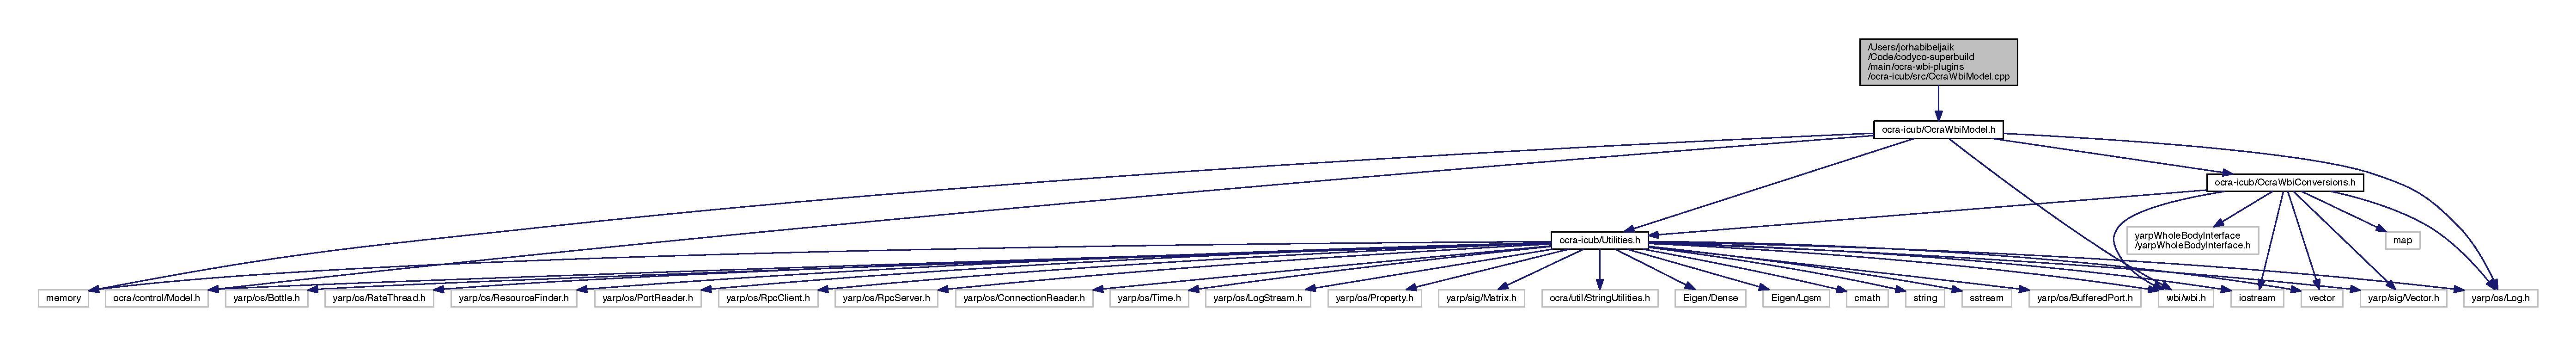
\includegraphics[width=350pt]{OcraWbiModel_8cpp__incl}
\end{center}
\end{figure}
\subsection*{Classes}
\begin{DoxyCompactItemize}
\item 
struct \hyperlink{structOcraWbiModel_1_1OcraWbiModel__pimpl}{ocra\+\_\+icub\+::\+Ocra\+Wbi\+Model\+::\+Ocra\+Wbi\+Model\+\_\+pimpl}
\end{DoxyCompactItemize}
\subsection*{Macros}
\begin{DoxyCompactItemize}
\item 
\#define \hyperlink{OcraWbiModel_8cpp_a7f4e728fa0fd89911a2c60c42c0d4560}{A\+L\+L\+\_\+\+J\+O\+I\+N\+TS}~-\/1
\item 
\#define \hyperlink{OcraWbiModel_8cpp_a29de1200631802e23f75bbd14adcc082}{F\+R\+E\+E\+\_\+\+R\+O\+O\+T\+\_\+\+D\+OF}~6
\item 
\#define \hyperlink{OcraWbiModel_8cpp_a72cb22de2538ae949cc73fa3d7c33bdc}{C\+O\+M\+\_\+\+P\+O\+S\+\_\+\+D\+IM}~3
\item 
\#define \hyperlink{OcraWbiModel_8cpp_ab4a87cb824ceff256c6b8bce7701af58}{T\+R\+A\+N\+S\+\_\+\+R\+O\+T\+\_\+\+D\+IM}~6
\item 
\#define \hyperlink{OcraWbiModel_8cpp_afbb98f526272c46369f405eee4e9d9aa}{G\+R\+A\+V\+I\+T\+Y\+\_\+\+C\+O\+N\+S\+T\+A\+NT}~-\/9.\+81
\end{DoxyCompactItemize}
\subsection*{Typedefs}
\begin{DoxyCompactItemize}
\item 
typedef Eigen\+::\+Displacementd\+::\+Adjoint\+Matrix \hyperlink{OcraWbiModel_8cpp_a2ee3f7feea423a8bc6b8fbcea1d4e217}{Adjoint\+Matrix}
\end{DoxyCompactItemize}
\subsection*{Variables}
\begin{DoxyCompactItemize}
\item 
const double \hyperlink{OcraWbiModel_8cpp_a3cdc4ec85b339c11e5b34ce069bf7077}{g\+\_\+vector} \mbox{[}3\mbox{]} = \{0, 0, \hyperlink{OcraWbiModel_8cpp_afbb98f526272c46369f405eee4e9d9aa}{G\+R\+A\+V\+I\+T\+Y\+\_\+\+C\+O\+N\+S\+T\+A\+NT}\}
\end{DoxyCompactItemize}


\subsection{Detailed Description}
Implementation of ocra\+::\+Model using whole\+Body\+Interface. 

\begin{DoxyAuthor}{Author}
\href{http://www.ryanlober.com}{\tt Ryan Lober} 

\href{http://ahoarau.github.io}{\tt Antoine Hoarau} 
\end{DoxyAuthor}
\begin{DoxyDate}{Date}
Feb 2016 
\end{DoxyDate}
\begin{DoxyCopyright}{Copyright}
G\+NU General Public License. 
\end{DoxyCopyright}


\subsection{Macro Definition Documentation}
\hypertarget{OcraWbiModel_8cpp_a7f4e728fa0fd89911a2c60c42c0d4560}{}\label{OcraWbiModel_8cpp_a7f4e728fa0fd89911a2c60c42c0d4560} 
\index{Ocra\+Wbi\+Model.\+cpp@{Ocra\+Wbi\+Model.\+cpp}!A\+L\+L\+\_\+\+J\+O\+I\+N\+TS@{A\+L\+L\+\_\+\+J\+O\+I\+N\+TS}}
\index{A\+L\+L\+\_\+\+J\+O\+I\+N\+TS@{A\+L\+L\+\_\+\+J\+O\+I\+N\+TS}!Ocra\+Wbi\+Model.\+cpp@{Ocra\+Wbi\+Model.\+cpp}}
\subsubsection{\texorpdfstring{A\+L\+L\+\_\+\+J\+O\+I\+N\+TS}{ALL\_JOINTS}}
{\footnotesize\ttfamily \#define A\+L\+L\+\_\+\+J\+O\+I\+N\+TS~-\/1}

\hypertarget{OcraWbiModel_8cpp_a72cb22de2538ae949cc73fa3d7c33bdc}{}\label{OcraWbiModel_8cpp_a72cb22de2538ae949cc73fa3d7c33bdc} 
\index{Ocra\+Wbi\+Model.\+cpp@{Ocra\+Wbi\+Model.\+cpp}!C\+O\+M\+\_\+\+P\+O\+S\+\_\+\+D\+IM@{C\+O\+M\+\_\+\+P\+O\+S\+\_\+\+D\+IM}}
\index{C\+O\+M\+\_\+\+P\+O\+S\+\_\+\+D\+IM@{C\+O\+M\+\_\+\+P\+O\+S\+\_\+\+D\+IM}!Ocra\+Wbi\+Model.\+cpp@{Ocra\+Wbi\+Model.\+cpp}}
\subsubsection{\texorpdfstring{C\+O\+M\+\_\+\+P\+O\+S\+\_\+\+D\+IM}{COM\_POS\_DIM}}
{\footnotesize\ttfamily \#define C\+O\+M\+\_\+\+P\+O\+S\+\_\+\+D\+IM~3}

\hypertarget{OcraWbiModel_8cpp_a29de1200631802e23f75bbd14adcc082}{}\label{OcraWbiModel_8cpp_a29de1200631802e23f75bbd14adcc082} 
\index{Ocra\+Wbi\+Model.\+cpp@{Ocra\+Wbi\+Model.\+cpp}!F\+R\+E\+E\+\_\+\+R\+O\+O\+T\+\_\+\+D\+OF@{F\+R\+E\+E\+\_\+\+R\+O\+O\+T\+\_\+\+D\+OF}}
\index{F\+R\+E\+E\+\_\+\+R\+O\+O\+T\+\_\+\+D\+OF@{F\+R\+E\+E\+\_\+\+R\+O\+O\+T\+\_\+\+D\+OF}!Ocra\+Wbi\+Model.\+cpp@{Ocra\+Wbi\+Model.\+cpp}}
\subsubsection{\texorpdfstring{F\+R\+E\+E\+\_\+\+R\+O\+O\+T\+\_\+\+D\+OF}{FREE\_ROOT\_DOF}}
{\footnotesize\ttfamily \#define F\+R\+E\+E\+\_\+\+R\+O\+O\+T\+\_\+\+D\+OF~6}

\hypertarget{OcraWbiModel_8cpp_afbb98f526272c46369f405eee4e9d9aa}{}\label{OcraWbiModel_8cpp_afbb98f526272c46369f405eee4e9d9aa} 
\index{Ocra\+Wbi\+Model.\+cpp@{Ocra\+Wbi\+Model.\+cpp}!G\+R\+A\+V\+I\+T\+Y\+\_\+\+C\+O\+N\+S\+T\+A\+NT@{G\+R\+A\+V\+I\+T\+Y\+\_\+\+C\+O\+N\+S\+T\+A\+NT}}
\index{G\+R\+A\+V\+I\+T\+Y\+\_\+\+C\+O\+N\+S\+T\+A\+NT@{G\+R\+A\+V\+I\+T\+Y\+\_\+\+C\+O\+N\+S\+T\+A\+NT}!Ocra\+Wbi\+Model.\+cpp@{Ocra\+Wbi\+Model.\+cpp}}
\subsubsection{\texorpdfstring{G\+R\+A\+V\+I\+T\+Y\+\_\+\+C\+O\+N\+S\+T\+A\+NT}{GRAVITY\_CONSTANT}}
{\footnotesize\ttfamily \#define G\+R\+A\+V\+I\+T\+Y\+\_\+\+C\+O\+N\+S\+T\+A\+NT~-\/9.\+81}

\hypertarget{OcraWbiModel_8cpp_ab4a87cb824ceff256c6b8bce7701af58}{}\label{OcraWbiModel_8cpp_ab4a87cb824ceff256c6b8bce7701af58} 
\index{Ocra\+Wbi\+Model.\+cpp@{Ocra\+Wbi\+Model.\+cpp}!T\+R\+A\+N\+S\+\_\+\+R\+O\+T\+\_\+\+D\+IM@{T\+R\+A\+N\+S\+\_\+\+R\+O\+T\+\_\+\+D\+IM}}
\index{T\+R\+A\+N\+S\+\_\+\+R\+O\+T\+\_\+\+D\+IM@{T\+R\+A\+N\+S\+\_\+\+R\+O\+T\+\_\+\+D\+IM}!Ocra\+Wbi\+Model.\+cpp@{Ocra\+Wbi\+Model.\+cpp}}
\subsubsection{\texorpdfstring{T\+R\+A\+N\+S\+\_\+\+R\+O\+T\+\_\+\+D\+IM}{TRANS\_ROT\_DIM}}
{\footnotesize\ttfamily \#define T\+R\+A\+N\+S\+\_\+\+R\+O\+T\+\_\+\+D\+IM~6}



\subsection{Typedef Documentation}
\hypertarget{OcraWbiModel_8cpp_a2ee3f7feea423a8bc6b8fbcea1d4e217}{}\label{OcraWbiModel_8cpp_a2ee3f7feea423a8bc6b8fbcea1d4e217} 
\index{Ocra\+Wbi\+Model.\+cpp@{Ocra\+Wbi\+Model.\+cpp}!Adjoint\+Matrix@{Adjoint\+Matrix}}
\index{Adjoint\+Matrix@{Adjoint\+Matrix}!Ocra\+Wbi\+Model.\+cpp@{Ocra\+Wbi\+Model.\+cpp}}
\subsubsection{\texorpdfstring{Adjoint\+Matrix}{AdjointMatrix}}
{\footnotesize\ttfamily typedef Eigen\+::\+Displacementd\+::\+Adjoint\+Matrix \hyperlink{OcraWbiModel_8cpp_a2ee3f7feea423a8bc6b8fbcea1d4e217}{Adjoint\+Matrix}}



\subsection{Variable Documentation}
\hypertarget{OcraWbiModel_8cpp_a3cdc4ec85b339c11e5b34ce069bf7077}{}\label{OcraWbiModel_8cpp_a3cdc4ec85b339c11e5b34ce069bf7077} 
\index{Ocra\+Wbi\+Model.\+cpp@{Ocra\+Wbi\+Model.\+cpp}!g\+\_\+vector@{g\+\_\+vector}}
\index{g\+\_\+vector@{g\+\_\+vector}!Ocra\+Wbi\+Model.\+cpp@{Ocra\+Wbi\+Model.\+cpp}}
\subsubsection{\texorpdfstring{g\+\_\+vector}{g\_vector}}
{\footnotesize\ttfamily const double g\+\_\+vector\mbox{[}3\mbox{]} = \{0, 0, \hyperlink{OcraWbiModel_8cpp_afbb98f526272c46369f405eee4e9d9aa}{G\+R\+A\+V\+I\+T\+Y\+\_\+\+C\+O\+N\+S\+T\+A\+NT}\}}


\hypertarget{Utilities_8cpp}{}\section{/\+Users/jorhabibeljaik/\+Code/codyco-\/superbuild/main/ocra-\/wbi-\/plugins/ocra-\/icub/src/\+Utilities.cpp File Reference}
\label{Utilities_8cpp}\index{/\+Users/jorhabibeljaik/\+Code/codyco-\/superbuild/main/ocra-\/wbi-\/plugins/ocra-\/icub/src/\+Utilities.\+cpp@{/\+Users/jorhabibeljaik/\+Code/codyco-\/superbuild/main/ocra-\/wbi-\/plugins/ocra-\/icub/src/\+Utilities.\+cpp}}


Some useful tools for the ocra-\/icub lib.  


{\ttfamily \#include \char`\"{}ocra-\/icub/\+Utilities.\+h\char`\"{}}\newline
\subsection*{Functions}
\begin{DoxyCompactItemize}
\item 
void \hyperlink{Utilities_8cpp_a666768e3a20bb81b9df67e3814a783bb}{get\+Nominal\+Posture} (const ocra\+::\+Model \&model, Eigen\+::\+Vector\+Xd \&q)
\item 
void \hyperlink{Utilities_8cpp_aeeff320b9cc14a9a7cf72fcfbdada2f6}{get\+Home\+Posture} (const ocra\+::\+Model \&model, Eigen\+::\+Vector\+Xd \&q)
\end{DoxyCompactItemize}


\subsection{Detailed Description}
Some useful tools for the ocra-\/icub lib. 

This file is for all the various macros and helper classes that are generic to ocra-\/icub. It is also a place for all the repeated includes like standard stl includes etc. \begin{DoxyAuthor}{Author}
\href{http://www.ryanlober.com}{\tt Ryan Lober} 
\end{DoxyAuthor}
\begin{DoxyDate}{Date}
Feb 2016 
\end{DoxyDate}
\begin{DoxyCopyright}{Copyright}
G\+NU General Public License. 
\end{DoxyCopyright}


\subsection{Function Documentation}
\hypertarget{Utilities_8cpp_aeeff320b9cc14a9a7cf72fcfbdada2f6}{}\label{Utilities_8cpp_aeeff320b9cc14a9a7cf72fcfbdada2f6} 
\index{Utilities.\+cpp@{Utilities.\+cpp}!get\+Home\+Posture@{get\+Home\+Posture}}
\index{get\+Home\+Posture@{get\+Home\+Posture}!Utilities.\+cpp@{Utilities.\+cpp}}
\subsubsection{\texorpdfstring{get\+Home\+Posture()}{getHomePosture()}}
{\footnotesize\ttfamily void get\+Home\+Posture (\begin{DoxyParamCaption}\item[{const ocra\+::\+Model \&}]{model,  }\item[{Eigen\+::\+Vector\+Xd \&}]{q }\end{DoxyParamCaption})}

\hypertarget{Utilities_8cpp_a666768e3a20bb81b9df67e3814a783bb}{}\label{Utilities_8cpp_a666768e3a20bb81b9df67e3814a783bb} 
\index{Utilities.\+cpp@{Utilities.\+cpp}!get\+Nominal\+Posture@{get\+Nominal\+Posture}}
\index{get\+Nominal\+Posture@{get\+Nominal\+Posture}!Utilities.\+cpp@{Utilities.\+cpp}}
\subsubsection{\texorpdfstring{get\+Nominal\+Posture()}{getNominalPosture()}}
{\footnotesize\ttfamily void get\+Nominal\+Posture (\begin{DoxyParamCaption}\item[{const ocra\+::\+Model \&}]{model,  }\item[{Eigen\+::\+Vector\+Xd \&}]{q }\end{DoxyParamCaption})}


\hypertarget{README_8md}{}\section{R\+E\+A\+D\+M\+E.\+md File Reference}
\label{README_8md}\index{R\+E\+A\+D\+M\+E.\+md@{R\+E\+A\+D\+M\+E.\+md}}

%--- End generated contents ---

% Index
\backmatter
\newpage
\phantomsection
\clearemptydoublepage
\addcontentsline{toc}{chapter}{Index}
\printindex

\end{document}
